%% abtex2-modelo-trabalho-academico.tex, v-1.9.6 laurocesar
%% Copyright 2012-2016 by abnTeX2 group at http://www.abntex.net.br/ 
%%
%% This work may be distributed and/or modified under the
%% conditions of the LaTeX Project Public License, either version 1.3
%% of this license or (at your option) any later version.
%% The latest version of this license is in
%%   http://www.latex-project.org/lppl.txt
%% and version 1.3 or later is part of all distributions of LaTeX
%% version 2005/12/01 or later.
%%
%% This work has the LPPL maintenance status `maintained'.
%% 
%% The Current Maintainer of this work is the abnTeX2 team, led
%% by Lauro César Araujo. Further information are available on 
%% http://www.abntex.net.br/
%% 
%% This work consists of the files abntex2-modelo-trabalho-academico.tex,
%% abntex2-modelo-include-comandos and abntex2-modelo-references.bib
%%

% ------------------------------------------------------------------------
% ------------------------------------------------------------------------
% abnTeX2: Modelo de Trabalho Academico (tese de doutorado, dissertacao de
% mestrado e trabalhos monograficos em geral) em conformidade com 
% ABNT NBR 14724:2011: Informacao e documentacao - Trabalhos academicos -
% Apresentacao
% ------------------------------------------------------------------------
% ------------------------------------------------------------------------

\documentclass[
	% -- opções da classe memoir --
	12pt,				% tamanho da fonte
	openright,			% capítulos começam em pág ímpar (insere página vazia caso preciso)
	twoside,			% para impressão em recto e verso. Oposto a oneside
	a4paper,			% tamanho do papel. 
	% -- opções da classe abntex2 --
	%chapter=TITLE,		% títulos de capítulos convertidos em letras maiúsculas
	%section=TITLE,		% títulos de seções convertidos em letras maiúsculas
	%subsection=TITLE,	% títulos de subseções convertidos em letras maiúsculas
	%subsubsection=TITLE,% títulos de subsubseções convertidos em letras maiúsculas
	% -- opções do pacote babel --
	english,			% idioma adicional para hifenização
	french,				% idioma adicional para hifenização
	spanish,			% idioma adicional para hifenização
	brazil				% o último idioma é o principal do documento
	]{abntex2}

% ---
% Pacotes básicos 
% ---
\usepackage{lmodern}			% Usa a fonte Latin Modern			
\usepackage[T1]{fontenc}		% Selecao de codigos de fonte.
\usepackage[utf8]{inputenc}		% Codificacao do documento (conversão automática dos acentos)
\usepackage{lastpage}			% Usado pela Ficha catalográfica
\usepackage{indentfirst}		% Indenta o primeiro parágrafo de cada seção.
\usepackage{color}				% Controle das cores
\usepackage{graphicx}			% Inclusão de gráficos
\usepackage{microtype} 			% para melhorias de justificação
\usepackage{todonotes}			% notas
\usepackage{tgpagella}			% fonte palatino	
\usepackage{mathpazo} 			% fonte palatino
\usepackage{url}
%\usepackage[font={small}]{caption}
%\usepackage[font=sf, small]{caption}




 \usepackage{caption}
 \captionsetup{%
  font={footnotesize}, % small font size
  labelfont={bf,sf},      % label in bold, sans-serif
  singlelinecheck=false, % centered single-lined captions
  font=sf,             % indention=1cm,
  labelsep={colon},         % default separator: none, colon, period, space, quad, newline, endash
}
%\usepackage[font=sf]{floatrow}

% ---
		
% ---
% Pacotes adicionais, usados apenas no âmbito do Modelo Canônico do abnteX2
% ---
\usepackage{lipsum}				% para geração de dummy text
% ---

% ---
% Pacotes de citações
% ---
\usepackage[brazilian,hyperpageref]{backref}	 % Paginas com as citações na bibl
\usepackage[alf]{abntex2cite}	% Citações padrão ABNT
\graphicspath{{pictures/}}             % caminho das figuras (recomendável)
%\bibliographystyle{abnt-num}% --- 
% CONFIGURAÇÕES DE PACOTES
% --- 

% ---
% Configurações do pacote backref
% Usado sem a opção hyperpageref de backref
\renewcommand{\backrefpagesname}{Citado na(s) página(s):~}
% Texto padrão antes do número das páginas
\renewcommand{\backref}{}
% Define os textos da citação
\renewcommand*{\backrefalt}[4]{
	\ifcase #1 %
		Nenhuma citação no texto.%
	\or
		Citado na página #2.%
	\else
		Citado #1 vezes nas páginas #2.%
	\fi}%
% ---

% ---
% Informações de dados para CAPA e FOLHA DE ROSTO
% ---
\titulo{Música em Rede: \\experimentos em interação musical}
\autor{Ariane de Souza Stolfi}
\local{São Paulo}
\data{2018}
\orientador{Fernando Henrique de Oliveira Iazzetta}
%\coorientador{Equipe \abnTeX}
\instituicao{%
  Universidade de São Paulo
  \par
  Escola de Comunicações e Artes
  \par
  Programa de Pós-Graduação em Música}
\tipotrabalho{Tese (Doutorado)}
% O preambulo deve conter o tipo do trabalho, o objetivo, 
% o nome da instituição e a área de concentração 
\preambulo{Tese apresentada à Escola de Comunicação e Artes para obtenção do título de Doutor em Música. Área de concentração: Processos de Criação Musical.}
%Linha de pesquisa: Sonologia
% ---


% ---
% Configurações de aparência do PDF final

% alterando o aspecto da cor azul
\definecolor{blue}{RGB}{100,100,100}

% informações do PDF
\makeatletter
\hypersetup{
     	%pagebackref=true,
		pdftitle={\@title}, 
		pdfauthor={\@author},
    	pdfsubject={\imprimirpreambulo},
	    pdfcreator={LaTeX with abnTeX2},
		pdfkeywords={abnt}{latex}{abntex}{abntex2}{trabalho acadêmico}, 
		colorlinks=true,       		% false: boxed links; true: colored links
    	linkcolor=blue,          	% color of internal links
    	citecolor=blue,        		% color of links to bibliography
    	filecolor=magenta,      		% color of file links
		urlcolor=blue,
		bookmarksdepth=4
}
\makeatother
% --- 

% --- 
% Espaçamentos entre linhas e parágrafos 
% --- 

% O tamanho do parágrafo é dado por:
\setlength{\parindent}{0cm}

% Controle do espaçamento entre um parágrafo e outro:
\setlength{\parskip}{1em}  % tente também \onelineskip

% ---
% compila o indice
% ---
\makeindex
% ---

% ----
% Início do documento
% ----
\begin{document}

% Seleciona o idioma do documento (conforme pacotes do babel)
%\selectlanguage{english}
\selectlanguage{brazil}

% Retira espaço extra obsoleto entre as frases.
\frenchspacing 

% ----------------------------------------------------------
% ELEMENTOS PRÉ-TEXTUAIS
% ----------------------------------------------------------
% \pretextual

% ---
% Capa
% ---
\imprimircapa
% ---

% ---
% Folha de rosto
% (o * indica que haverá a ficha bibliográfica)
% ---
\imprimirfolhaderosto*
% ---

% ---
% Inserir a ficha bibliografica
% ---

% Isto é um exemplo de Ficha Catalográfica, ou ``Dados internacionais de
% catalogação-na-publicação''. Você pode utilizar este modelo como referência. 
% Porém, provavelmente a biblioteca da sua universidade lhe fornecerá um PDF
% com a ficha catalográfica definitiva após a defesa do trabalho. Quando estiver
% com o documento, salve-o como PDF no diretório do seu projeto e substitua todo
% o conteúdo de implementação deste arquivo pelo comando abaixo:
%
% \begin{fichacatalografica}
%     \includepdf{fig_ficha_catalografica.pdf}
% \end{fichacatalografica}

\begin{fichacatalografica}
	\sffamily
	\vspace*{\fill}					% Posição vertical
	\begin{center}					% Minipage Centralizado
	\fbox{\begin{minipage}[c][8cm]{13.5cm}		% Largura
	\small
	\imprimirautor
	%Sobrenome, Nome do autor
	
	\hspace{0.5cm} \imprimirtitulo  / \imprimirautor. --
	\imprimirlocal, \imprimirdata-
	
	\hspace{0.5cm} \pageref{LastPage} p. : il. (algumas color.) ; 30 cm.\\
	
	\hspace{0.5cm} \imprimirorientadorRotulo~\imprimirorientador\\
	
	\hspace{0.5cm}
	\parbox[t]{\textwidth}{\imprimirtipotrabalho~--~\imprimirinstituicao,
	\imprimirdata.}\\
	
	\hspace{0.5cm}
		1. Música.
		2. Design de interface.
		3. Improvisação livre.
		I. Fernando Henrique de Oliveira Iazzetta.
		II. Universidade de São Paulo.
		III. Escola de Comunicação e Artes.
		IV. Práticas de luteria na música experimental brasileira 			
	\end{minipage}}
	\end{center}
\end{fichacatalografica}
% ---

% ---
% Inserir errata
% ---
%\begin{errata}
%Elemento opcional da %\citeonline[4.2.1.2]{NBR14724:2011}. Exemplo:

%\vspace{\onelineskip}

%FERRIGNO, C. R. A. \textbf{Tratamento de neoplasias ósseas apendiculares com
%reimplantação de enxerto ósseo autólogo autoclavado associado ao plasma
%rico em plaquetas}: estudo crítico na cirurgia de preservação de membro em
%cães. 2011. 128 f. Tese (Livre-Docência) - Faculdade de Medicina Veterinária e
%Zootecnia, Universidade de São Paulo, São Paulo, 2011.

%\begin{table}[htb]
%\center
%\footnotesize
%\begin{tabular}{|p{1.4cm}|p{1cm}|p{3cm}|p{3cm}|}
%  \hline
%   \textbf{Folha} & \textbf{Linha}  & \textbf{Onde se lê}  & \textbf{Leia-se}  \\
%    \hline
%    1 & 10 & auto-conclavo & autoconclavo\\
%   \hline
%\end{tabular}
%\end{table}

%\end{errata}
% ---

% ---
% Inserir folha de aprovação
% ---

% Isto é um exemplo de Folha de aprovação, elemento obrigatório da NBR
% 14724/2011 (seção 4.2.1.3). Você pode utilizar este modelo até a aprovação
% do trabalho. Após isso, substitua todo o conteúdo deste arquivo por uma
% imagem da página assinada pela banca com o comando abaixo:
%
% \includepdf{folhadeaprovacao_final.pdf}
%
\begin{folhadeaprovacao}

  \begin{center}
    {\ABNTEXchapterfont\large\imprimirautor}

    \vspace*{\fill}\vspace*{\fill}
    \begin{center}
      \ABNTEXchapterfont\bfseries\Large\imprimirtitulo
    \end{center}
    \vspace*{\fill}
    
    \hspace{.45\textwidth}
    \begin{minipage}{.5\textwidth}
        \imprimirpreambulo
    \end{minipage}%
    \vspace*{\fill}
   \end{center}
        
   Trabalho aprovado. \imprimirlocal,    de           de 2018:
%
   \assinatura{\textbf{\imprimirorientador} \\ Orientador} 
   \assinatura{\textbf{Professor} \\ Convidado 1}
   \assinatura{\textbf{Professor} \\ Convidado 2}
   \assinatura{\textbf{Professor} \\ Convidado 3}
   \assinatura{\textbf{Professor} \\ Convidado 4}
%      
   \begin{center}
    \vspace*{0.5cm}
    {\large\imprimirlocal}
    \par
    {\large\imprimirdata}
    \vspace*{1cm}
  \end{center}
  
\end{folhadeaprovacao}

% ---

% ---
% Dedicatória
% ---pdf
\begin{dedicatoria}
   \vspace*{\fill}
   \begin{flushright}
   \textit{A quem queiser tocar}
   \end{flushright}
   \vspace*{\fill}
\end{dedicatoria}

% ---

% ---
% Agradecimentos
% ---
%\begin{agradecimentos}
%
% À toda a minha família, agradeço pelo apoio e instigação constante, às Júlias e ao pequeno Miguel, agradeço pela paciência e pelo amor em todos os momentos;
%
%A todos os entrevistados e todas as pessoas que colaboraram com dicas valiosas ao longo do trabalho: Löis Lancaster, Eric Marke, Scott Lee, Nelson Ribeiro, George Romano, Marcelo Conter, Eduardo Santos, 
%
% A todas as professoras e professores que tive a sorte de encontrar pelo caminho e ter como amigos, em especial a Paulo Lima, Carlos Sandroni, John Murphy, Carlos Palombini por terem mostrado os caminhos e também por terem me ajudado a permanecer pesquisando.

% Aos meus companheiros do Mombojó, Alessandra Leão e banda, todas as irmãs e irmãos da graxa e da música pela alegria de trabalhar

%A Fernando Iazzetta pela paciência, pela amizade e pela inspiração;

% A Tony da Gatorra pela generosidade de abrir seu mundo e compartilhar suas ideias e sua música não só comigo;
%
%\end{agradecimentos}

% ---

% ---
% Epígrafe
% ---
\begin{epigrafe}
    \vspace*{\fill}
	\begin{flushright}
		\textit{Alegria é a prova dos nove \\(Oswald de andrade)}
	\end{flushright}
\end{epigrafe}
% ---

% ---
% RESUMOS
% ---

% resumo em português
\setlength{\absparsep}{18pt} % ajusta o espaçamento dos parágrafos do resumo
\begin{resumo}


%Este trabalho faz um levantamento da produção brasileira de luteria experimental, com ênfase na produção realizada ao longo das últimas duas décadas. Inicialmente é delineado um panorama de referências relacionadas com este tido de produção na literatura europeia e estadunidense, assim como discutida a atuação de alguns artistas e criadores fundamentais para o estabelecimento de práticas de luteria experimental no século XX. No segundo capítulo faço um levantamento de referências sobre este tipo de produção no Brasil, assim como relaciono artistas em atividade no país nos últimos 20 anos, detalhando na maior parte dos casos algumas de suas obras. Partindo deste panorama, realizo um estudo mais aprofundado sobre o instrumento conhecido por gatorra, fabricado por Tony da Gatorra, artesão, técnico em eletrônica e músico gaúcho que criou seu instrumento nos anos 1990 a partir de materiais de sucata, componentes eletrônicos reaproveitados e da combinação de projetos de circuitos eletrônicos geradores de som. Por fim, relaciono a produção estudada com referenciais que lidam com a noção de cultura material, alguns dos quais já realizam uma aproximação com a atividade musical e artística.


 \textbf{Palavras-chave}: Música experimental. Luteria digital, Música Interativa. \textit{WebAudio}. Música Ubíqua. 
\end{resumo}

% resumo em inglês
\begin{resumo}[Abstract]
\begin{otherlanguage*}{english}
%This work presents a survey on the Brazilian production of experimental lutherie, with emphasis on the production over the last two decades. A framework of references related to this production in the European and American literature is outlined as an introduction, as well as the works of some key artists and creators whose production influenced experimental instrument building practices in the 20th century. In the second chapter I make a survey of references on this type of production in Brazil, as well a profile of artists active in the country for the last 20 years, detailing in most cases some of his works. Based on this outline, I carry out a more detailed study on the instrument known as gatorra, manufactured by Tony da Gatorra, an artisan, technician and musician who created his instrument in the 1990s from scrap materials, reused electronic components and the combination of electronic circuits sound generators. Finally, I relate the production studied with references that deal with the notion of material culture, some of which already make an approximation with musical and artistic activity.


   \vspace{\onelineskip}
 
   \noindent 
   %\textbf{Keywords}: Experimental Music. Experimental Lutherie. Readymade. \textit{Gambiarra}. Technological desobedience. Material culture. Gatorra.
 \end{otherlanguage*}
\end{resumo}

% resumo em francês 
%\begin{resumo}[Résumé]
% \begin{otherlanguage*}{french}
%    Il s'agit d'un résumé en français.
 
%   \textbf{Mots-clés}: latex. abntex. publication de textes.
% \end{otherlanguage*}
%\end{resumo}

% resumo em espanhol
%\begin{resumo}[Resumen]
% \begin{otherlanguage*}{spanish}
%   Este es el resumen en español.
  
%   \textbf{Palabras clave}: latex. abntex. publicación de textos.
% \end{otherlanguage*}
%\end{resumo}
% ---

% ---
% inserir lista de ilustrações
% ---
\pdfbookmark[0]{\listfigurename}{lof}
\listoffigures*
\cleardoublepage
% ---

% ---
% inserir lista de tabelas
% ---
%\pdfbookmark[0]{\listtablename}{lot}
%\listoftables*
%\cleardoublepage
% ---

% ---
% inserir lista de abreviaturas e siglas
% ---
\begin{siglas}
%  \item[ABNT] Associação Brasileira de Normas Técnicas
%  \item[abnTeX] ABsurdas Normas para TeX
\item[W3C] \textit{World Wide Web Consortium}, entidade que define os padrões das linguages web.

\item[FFT] \textit{Fast Fourier Transform}, transformada rápida de Fourrier.
\item[SVG] \textit{Standard Vector Graphics}, ou ``faça você mesmo'' mais especificamente aplicado à construção de circuitos eletrônicos.
\item[MIDI] \textit{Musical Instrument Digital Interface}, Interface Digital de Instrumentos Musicais, um protocolo para comunicaçnao entre instrumentos digitais.
\item[HTML] \textit{HyperText Markup Language}, linguagem de marcação para formatação de páginas web.
\item[CSS] \textit{Cascading Stylesheets}, linguagem de estilização de páginas web.
\item[IRCAM] \textit{IRCAM}, instituição francesa dedicada à pesquisa e à criação de música contemporânea.
\item[FAU] \textit{Faculdade de Arquitetura e Urbanismo da Universidade de São Paulo}
\item[CC] \textit{Creative Commons}, sistema de licensas livres para conteúdo criativo. 
\item[IHC] \textit{Interação Humano Computador}
\item[NIME] Conferência New Interfaces for Musical Expression
\item[NuSom] Núcleo de estudos em sonologia da Universidade de São Paulo
\item[USP] Universidade de São Paulo
\item[QMUL] \textit{Queen Mary University of London}, sistema doméstico de gravação e reprodução de vídeo
\end{siglas}
% ---

% ---
% inserir lista de símbolos
% ---
%\begin{simbolos}
%  \item[$ \Gamma $] Letra grega Gama
%  \item[$ \Lambda $] Lambda
%  \item[$ \zeta $] Letra grega minúscula zeta
%  \item[$ \in $] Pertence
%\end{simbolos}
% ---

% ---
% inserir o sumario
% ---
\pdfbookmark[0]{\contentsname}{toc}
\tableofcontents*
\cleardoublepage
% ---



% ----------------------------------------------------------
% ELEMENTOS TEXTUAIS
% ----------------------------------------------------------
\textual

% !TEX root = tese.tex


\chapter*{Introdução}
\addcontentsline{toc}{chapter}{Introdução}
\label{ch:intro}

Esta pesquisa tem vários pontos de partida. Como um projeto transdisciplinar, entre campos como Música, Design e Computação Musical, parte de uma pesquisa anterior de investigação das tecnologias que dão suporte à web, desde o trabalho final de graduação na Faculdade de Arquitetura e Urbanismo da Universidade de São Paulo (FAU), um dicionário de linguagens de marcação e programação para web (HTML, CSS e JavaScript), que continuou no mestrado\footnote{Com a dissertação ``World Wide Web: Forma aparente e forma oculta'', procurei investigar história, processos e metodologias para o design de websites, com o sentido de aproximar os campos de atuação de designers e programadores}. Parte também de uma prática de produção, edição e gravação experimental de música e do trabalho junto a diversos grupos e coletivos em  práticas artísticas diversas, parte delas organizadas no acervo da página Finetanks.com que mantenho desde 2005.  
    Esta tese, surge em parte como um desejo de síntese entre essas diversas práticas e interesses, no campo do design, programação e música, de um desejo de investigar os potenciais de exploração de tecnologias web para criação musical. 
    
    
    Filósofos da sociedade pós-industrial como Daniel Bell (1979) \footnote{\cite{bell1979thinking}} relacionam o processo de digitalização da informação e dos meios de comunicação com a emergência de uma sociedade pós-industrial, onde a ``a informação se tornou o recurso estratégico e transformador na sociedade como o trabalho e o capital foram recursos estratégicos e transformadores na sociedade industrial'' \footnote{\cite[26]{bell1979thinking}}. Neste contexto, os sistemas de comunicação se tornam a principal estrutura de amarração e unificação da sociedade. Bell, que Richard Barbrook \footnote{\cite{barbrook1999cyber}} considera um dos principais expoentes da esquerda estadunidense da guerra fria, já apontava as potencialidades da criação de uma rede mundial de computadores como catalisador de interações interpessoais e como ampliadora das ``arenas onde ocorrem as ações sociais" \footnote{\cite[22]{bell1979thinking}}. Bell, desenvolve essa noção de ``sociedade da informação'' a partir de idéias propostas por Marshall McLuhan, difundidas principalmente no livro ``Os meios de comunicação como extensões do homem''\footnote{\cite{luhan1964marshall}}, de que a sociedade se  transforma a cada mudança ocorrida nas tecnologias e nos meios de comunicação. 
    
    A internet pode ser considerada uma espécie de ``meio de meios'' \footnote{\cite[5]{Levinson2001}}, que começou como um sistema de troca de informação, onde imperava principalmente o texto e passou gradualmente a ser suporte para diversos outros  meios de comunicação como telefone, rádio, cinema e televisão, um meta-meio, cujo conteúdo é, não só o conteúdo de todos meios anteriores, mas também o próprio usuário que coloca o conteúdo online \footnote{\cite[39]{Levinson2001}}. Quando Levinson analisava McLuhan em ``Digital McLuhan'', a internet ainda era um meio ainda dominado principalmente pela tecnologia da escrita, e sendo assim, dominado ainda pelo espaço visual. Apesar disso, a música foi um dos conteúdo significativos da rede, desde os primeiros sistemas de de compartilhamento de arquivos entre usuários, e o desenvolvimento constante das tecnologias, traz a ela cada vez mais novos potenciais acústicos.
    
Hoje, por exemplo enquanto escrevo esse texto, posso ouvir qualquer estação de rádio do mundo que faça \emph{live streaming} pela internet, através de um site como o Radio.garden (figura \ref{radiogarden}), por exemplo. O projeto coordenado pelo Netherlands Institute for Sound and Vision, reúne as estações de rádio em um mapa, e podemos acessá-las de qualquer lugar, e trocá-las com um girar do globo com o mouse, permitindo aos ouvintes a conexão com culturas distantes, ao explorar formas diversas de transmissão e identidades culturais de todo planeta \footnote{\cite{caroline2016radio}}. 

\begin{figure}[htb]
    \caption{\label{radiogarden} Radio.garden.}
    \begin{center}
        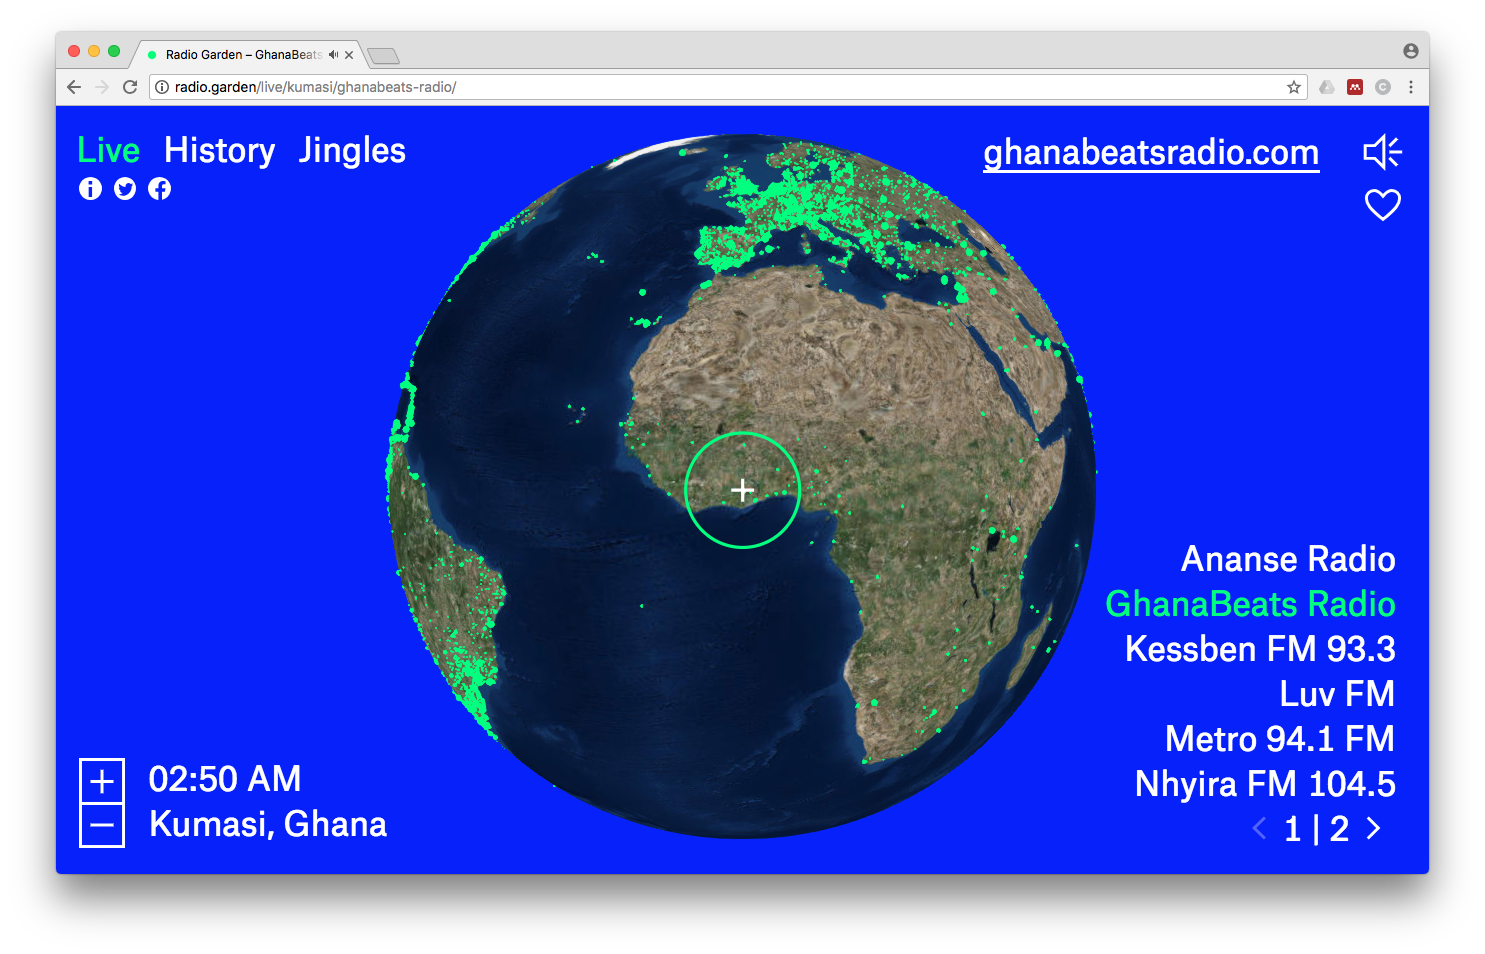
\includegraphics[width=1\linewidth]{pictures/radio_garden_2018-06-10.png}
    \end{center}
    \legend{Fonte: Screenshot da autora, 8 de junho de 2018}
    
\end{figure}
%\legend{Fonte: \citeonline[p. 24]{araujo2012}}

Posso também acessar uma base de dados extensiva da produção humana em música, cinema e televisão construída a partir do trabalho de pessoas em todo o planeta, reunida em grandes portais como o Youtube, onde segundo estatísticas atuais são depositadas 300 horas de conteúdo a cada minuto. Mas, como bem apontou a compositora Pauline Oliveros em ``Software for people", ``As mídias e a maior mobilidade obviamente acomodam mais informação, mas não necessariamente mais sabedoria"\footnote{\cite[179]{Oliveros2012}}. 

Teóricos da sociedade da informação, professavam que a internet teria um papel demiúrgico, que ``libertaria a humanidade sem qualquer necessidade de luta de classes" \footnote{\cite[275]{Barbrook2009}}. Para Howard Rheingold, da revista Wired, por exemplo, a internet também seria a ``curandeira da alientação social'', como aponta Barbrook:


\begin{citacao}
Em sua atualização da Nova Esquerda mcluhanista do início dos anos 1990, BBSs, MUDs, NT2, serviços de bate-papo instantâneos e servidores de lista de e-mail representavam os princípios da ágora eletrônica postos em prática: as “comunidades virtuais”. Fundada sobre o compartilhamento de informação e conhecimento, a Internet era uma das “ferramentas para pensar” que liberariam a humanidade da sociedade fabril fordista. \footnote{\cite[350]{Barbrook2009}}
\end{citacao}

Mas sob a neoliberal ``ideologia californiana'', a internet se transformou na apoteose do mercado \footnote{(idem, p. 353)}. Em ``Technologies of Freedom'', de 1983 Ithiel de Sola Pool codificava o que Barbrook chama de ``sua apropriação neoliberal do mluhanismo'':
\begin{citacao}
Ao invés de construir a ágora eletrônica, a convergência da mídia, das telecomunicações e da computação criava o mercado eletrônico. De programas de computadores a novelas, todas as formas de informação seriam logo negociadas como mercadorias pela Internet. Pela primeira vez, todos poderiam ser um empreendedor de mídia. \footnote{\cite[348]{Barbrook2009}}
\end{citacao}

Ele apnonta ainda que há quem inclusive culpe a mídia eletrônica por exacerbar uma série de de males da sociedade como: ``elitismo, pedofilia, terrorismo, deficiência educacional e solidão''. 

Não é difícil de concordar com essa visão. Uma simples tecnologia que permite ao usuário deixar sua opinião nas notícias dos grandes portais é suficiente para nos assombrar com o nível de barbárie latente na sociedade, a cada notícia veiculada na supostamente isenta ``grande mídia". Abre espaço para a voz do Zé Ninguém, como definido por Wilhelm Reich \footnote{\cite{reich1998escute}}, aquele ser de mentalidade tacanha, que ``está sempre do lado dos perseguidores'' (p. 27), que persegue mães solteiras, por serem imorais, ao mesmo tempo que cultua Jesus, que ``é tolerante com a sua própria religião mas com nenhuma outra (p.51)":

\begin{citacao}
como não tem memória para coisas que aconteceram há dez ou vinte anos, você ainda repete os mesmos disparates de dois mil anos atrás. Pior, você se agarra com unhas e dentes a absurdos como ``raça'', ``classe'', ``nação'' e à obrigação de seguir uma religião e reprimir sua desgraça. \footnote{\cite[101]{reich1998escute}}
\end{citacao}

No momento em que escrevo esta tese, passamos no Brasil por uma eleição onde o candidato vencedor explorou fortmente o apelo de notícias para uma população desinformada que pode acreditar nos maiores absurdos propagados pelas redes sociais. Produtores de notícias falsas por todo o mundo exploram deliberadamente recursos e algoritmos das redes sociais para propagar suas mensagens \footnote{\cite{Martens2018}}, que influenciam resultados políticos em diversos países.

Apesar disso, nós, que somos artistas, pesquisadores e pessoas que criam, não podemos nos sujeitar passivamente à essa visão apocalíptica de que a internet está nos levando à barbárie, e podemos pensar nos meios tecnológicos como ponto de partida para novas proposições éticas e estéticas. Concordamos com arquiteto e pintor Sérgio Ferro quando afirma: que a expressão humana na arte é ``pegar a necessidade histórica que está no material e trabalhá-la até o fundo", \footnote{\cite{FerroSergio2002}} e que isto é a própria essência da liberdade. Sendo operadores de cultura, não devemos negar a indústria cultural, mas como já apontava Eco (\citeyear{Eco1970}), ``Colocar se em relação dialética, ativa e consciente com os condicionamentos da indústria cultural''\footnote{\cite[14]{Eco1970}}. Para ele, esse é o único caminho possível para que o ``operador de cultura'' cumpra sua função. Para ele, as codições objetivas devem ser o ponto de partida para a nossa criação artística: 



\begin{citacao}
A nosso ver, se devemos operar \emph{em} e \emph{para} um mundo construído na medida humana, essa medida será individuada não adaptando o homem a essas condições de fato mas \emph{a partir dessas condições de fato}. O universo das comunicações de massa é -- reconheçamo-lo ou não -- o nosso universo; e se quisermos falar de valores, as condições objetivas das comunicações são aquelas fornecidas pela existência dos jornais, do rádio, da televisão, da música reproduzida e reproduzível, das novas formas de comunicação visiva e auditiva. Ninguém foge a essas condições, nem mesmo o virtuoso, que, indignado com a natureza inumana desse universo da informação, transmite o próprio protesto através dos canais de comunicação em massa, pelas colunas do grande diário, ou nas páginas do volume em \emph{paperback}, impresso em linotipo e difundido nos quiosques das estações.\footnote{\cite[13]{Eco1970}}

\end{citacao}

 Lev Manovich (\citeyear{Manovich2008}), artista que também teoriza sobre as ``novas mídias'', cunhou o termo ``infoestética'' \footnote{\cite{Manovich2008}}, para se referir às práticas culturais que surjem em resposta às questões da sociedade da informação, tirando sentido, trabalhando com ou produzindo conhecimento a partir da informação, examinando muitos campos culturais onde o emprego da computação deu origem a ``novas formas''. Se nossas condições objetivas nos colocam a realidade da internet e das mídias sociais como os meios de comunicação estruturantes das relações humanas atuais, pensar esses meios criticamente também é uma das tarefas dos artistas e produtores culturais. Em uma sociedade fortemente mediada por tecnologias de computação, a programação pode ser uma forma de potência, que permite ao agente atuar sobre a cultura da informação para além da posição de observador.

\subsection{Música como potência}
Dentre as demais formas de arte, consifero que a música é epecialmente potente. 

%literalmente pode se falar de potência sonora

O som é quase impossível de se bloquear, e sendo assim, a música tem a capacidade de atingir as pessoas circundantes de uma maneira geral e compulsória, uma vez que energia sonora é das mais difíceis de se conter em termos coletivos. É possível um indivíduo tampar seus próprios ouvidos, mas é muito difícil tapar os ouvidos alheios, e mesmo tapando os ouvidos, nunca haverá silêncio\footnote{É famoso o experimento de John Cage que 1951 entrou em uma câmara anecóica, onde supostamente haveria silêncio total. Ao invés de encontrar o silêncio, Cage ouviu os sons do seu sistema nervoro (agudo) e circulatório (\cite{Mauceri1997})}. Levinson (\citeyear{Levinson2001}) aponta que o som tem como característica``emanar de todos ambientes'', e enquanto a visão nos dá detalhes preciso, ponto-a-ponto do ambiente ao nosso redor, é a audição que ``nos mantém em contato com o mundo vinte e quatro horas por dia" \footnote{\cite[47]{Levinson2001}}. No ``Panorama setorial da cultura brasileira'', levantamento feito sob coordenação de Gise Jordão, levantamento 
 

Minha relação com a produção musical teve muita relação com um potencial de agregação que a música traz. Primeiro, como dj, organizando festas que eram essenciais para o financiamento do grêmio dos estudantes da FAU, depois, no Urbando, grupo de maracatu que intervinha também em atos estudantis. Sempre foi muito nítido pra mim o potencial de um tambor ou um xequerê como instrumento de organização de massas em atos, como instrumentos para colocar as pessoas em movimento. Não é atoa que os exércitos usam marchas como forma de elevar a moral dos soldados\footnote{Pauline Oliversos cita em ``Software for People'' (p. 99) que a música militar foi o primeiro tipo de música introduzida no Oriente pelo Ocidente. \cite{Oliveros2012}}, e que também as igrejas usam música para encantar os fiéis. O discurso verbal pode ser cansativo, o texto pode ser ignorado, enquanto a música é capaz de colocar uma multidão em uníssono. Em uma sociedade como a nossa, esse poder é exercido principalmente pela indústria cultural, que afasta esse sentido político que a música pode ter, convertendo tudo em mercadoria, como aponta Marilena Chauí no seu artigo ``Cultura e Democracia'': 

\begin{citacao}

Como cultura de massa, as obras de pensamento e de arte tendem: de expressivas, tornarem-se reprodutivas e repetitivas; de trabalho da criação, tornarem-se eventos para consumo; de experimentação do novo, tornarem-se consagração do consagrado pela moda e pelo consumo; de duradouras, tornarem-se parte do mercado da moda, passageiro, efêmero, sem passado e sem futuro; de formas de conhecimento que desvendam a realidade e instituem relações com o verdadeiro, tornarem-se dissimulação, ilusão falsificadora, publicidade e propaganda. mais do que isso. A chamada cultura de massa se apropria das obras culturais para consumi-las, devorá-las, destruí-las, nulificá-las em simulacros. Justamente porque o espetáculo se torna simulacro e o simulacro se põe como entretenimento, os meios de comunicação de massa transformam tudo em entretenimento (guerras, genocídios, greves, festas, cerimônias religiosas, tragédias, políticas, catástrofes naturais e das cidades, obras de arte, obras de pensamento). É isto o mercado cultural. \footnote{\cite[61]{MarilenaChaui2008}}
\end{citacao}

Uma cultura democrática, seria aquela, segundo ela, onde as pessoas tenham acesso aos meios de produção cultural, e não somente aos produtos de seu mercado. Tendo uma formação em arquitetura e design, e sendo assim de certo modo estranha ao contexto e aos códigos da música tradicional, foi fácil notar o alto grau de fechamento da cena musical, especialmente para mulheres, como aponta Pauline Oliveros no texto ``And don't call them Lady Composers" \footnote{\cite[48]{Oliveros2012}}. 

\subsection{Acesso}
Uma das coisas que colabora com esse hermetismo é a dificuldade de acesso aos instrumentos musicais, que podem ser muito caros, pesados ou de difícil manipulação. O acesso aos meios de produção certamente é uma das barreiras que afasta as pessoas de uma vivência musical cotidiana. Instrumentos musicais, equipamentos de áudio em geral e controladores, podem ser muito caros, complexos e de difícil manipulação\footnote{\cite{Fiebrink2007}}. A digitalização das tecnologias de produção musical, no entanto, tornou acessível aos usuários de computadores pessoais, tecnologias que só eram disponíveis para grandes estúdios musicais. A partir dos anos 80, isso causou um crescimento exponencial do engajamento da juventude com meios de produção musical digitais, como aponta Georgina Born \footnote{\cite[143]{Born2015}}, mas também causa a uma ``tecnofilia fetichista'' em relação a equipamentos e tecnologias \footnote{(idem, p. 145)}.

Como aponta Baudrillard em ``O sistema de objetos", ``os consumidores não têm acesso à igualdade diante do objeto depois da Revolução Industrial" \footnote{\cite[162]{Baudrillard2012}}. Podemos dizer que a revolução digital, tem permitido concentrar uma série de funcionalidades em gadgets como celulares ou laptops, cada vez menores e mais complexos, que exercem cada vez mais uma dominação dos sentidos individuais das pessoas – que ficam dependentes e absortas em complexas tramas de dados e dramas. O gadget para Baudrillard é um objeto que faz parte de um universo de delírio funcional, um tecnicismo excêntrico e formalismo gratuito, objetos tomados totalmente pelo imaginário, ou obsessões pura e simples, aberrações funcionais. \footnote{(idem p.121)}. 

Meu projeto parte de um desejo de libertação dessa dependência de toda uma uma parafernália tecnológica, concentrando esforços em desenvolver protótipos experimentais para produção musical em tecnologias para a rede, que possam ser acessadas pelas pessoas de seus aparelhos de uso cotidiano: computadores pessoais, aparelhos de celular. Soluções deste tipo poderiam ser mais acessíveis, já que um instrumento musical online poderia ser acessado por qualquer dispositivo que tenha acesso à internet -- gadgets que ganharam muito poder de processamento, nos quais já estamos absortos. 

Dessa forma, essa pesquisa se insere também em um campo que tem se configurado recentemete como Música Ubíqua, que segundo Keller (\citeyear{Keller2018}), tem como objetivo prover acesso à tecnologias para prática musical a um número maior de pessoas, ou ``uma nova maneira de promover a criação musical em contextos não antes acessíveis a empenhos artísticos''\footnote{\cite{Keller2018}}. Para isso, pesquisadores do campo tem investigado o uso de tecnologias web e o do uso de dispositivos móveis, como celulares para produção musical. 

 Além disso, tinha um desejo sobretudo de investigar novas formas de interface, por considerar que muitas das interfaces existentes, que são em maioria baseadas nas de equipamentos eletrônicos \footnote{\cite{Stolfi2016}}, também exigem a necessidade de saberes bastante específicos em tecnologias musicais, além de imporem certos parâmetros da música tradicional, como notas, timbres e tempos. 

Com o desenvolvimento da pesquisa, e o meu contínuo envolvimento com práticas musicais como a da improvisação livre, ``uma pragmática musical aberta à variação infinita em que os sistemas e as linguagens deixam de impor suas gramáticas abstratas e se renderem a um fazer fecundo" \footnote{\cite[2]{Costa2016}} esse desejo de construção de instrumentos genéricos foi se direcionando para a construção de instrumentos específicos para suprir necessidades pessoais musicais -- como é o caso do projeto Banda Aberta e o Playsound.space, projetos que desenvolvi nesta pesquisa e que descreverei mais à frente nesta tese -- sempre buscando portabilidade e facilidade de uso.


Além da questnao da materialidade dos intrumentos físicos, o acesso à prática musical também passa pela questão do domínio do ``gesto musical''. Na música tradicional, o gesto -- do performer ou do intérprete -- é tradicionalmente o gerador do som. O domínio do ato de tocar, principalmente instrumentos tradicionais, envolve um domínio de uma linguagem corporal que gera o som desejado de acordo com o desejo do musicista. Na música instrumental e vocal, sempre há um gesto físico que gera o som, o que não acontece necessariamente na música eletrônica \footnote{\cite[85]{Smalley1996}}. Isto é uma preocupação de quem desenvolve aplicativos para música interativa, como aponta Schnell (\citeyear{Schnell2013}): 


\begin{citacao}
Two principal concerns constitute the design of interactive audio applications and musical instruments of virtually any kind. One deals with creating real-time interactive sound processes and the other with the way these sound processes are influenced by the bodily movements and gestures of their players. In this sense, the essence of designing interactive audio applications lies in the creation of meaningful relationships between movement – or gestures – and sound. \footnote{\cite{Schnell2013}}
\end{citacao}
Essa questão também é discutida no âmbito das \emph{laptop orchestras}, como aponta Trueman (2007):
\begin{citacao}
Para a performer de \emph{laptop}, isso parece representar um grande problema. Se parecer que nós estamos simplesmente respondendo e-mail equanto geramos sons, o que que o ``ouvinte'' vai pensar de tudo? que tipo de performance sofrível que isso poderia possivelmente inspirar? Como pareceria uma dancinha de computadores no ar\footnote{Aqui uma referência a \emp{air-guitar}, quando se imita o gesto de um guitarrista}?
Mas talvez isso seja uma oportunidade ao invés de um problema, um desafio para o qual a orquestra de laptops é um ginásio socialmente carregado. Por um lado, nós podemos encarar de frente e se esforçar para criar instrumentos desafiadores que podem gerar sons que pareçam de certa forma tangíveis (mesmo acústicamente), relacionados à fisicalidade que eles exijam.\footnote{\cite[6]{Trueman2007}} 
%For the laptop performer, this seems to pose a
%deep problem. If we look like we are simply doing e-mail while generating sounds that provoke the motor-mimetic response of, say, striking an enormous hammer, what will the ‘listener’ make of it all? What kind of vicarious performance could this possibly inspire?What would the ‘air-laptop’ dance look like? 
%But perhaps this is an opportunity instead of a problem, a challenge for which the laptop orchestra is a musically and socially charged gymnasium. On the one hand, we can go at it head-on and endeavour to create challenging instruments that generate sounds which somehow seem tangibly (even acoustically) related to the physicality they demand.
\end{citacao}

A noção de virtuosidade, para Smalley ({\citeyear{Smalley1996}) é baseada na identificação de um controle consumado na articulação de morfologias sonoras. No seu modelo do espectro de sons, Smalley considera como sons musicais, aqueles gerados com intenção pelos homens. Mesmo sons naturais podem ser convertidos em música, desde que sejam resultado de uma agência humana. O campo da música eletroacústica foi responsável por inserir na música uma ampla gama de sons sintetizados e da natureza que não necessariamente podem nem ter tido uma existência material. Muitos trabalhos acusmáticos, inclusive, não possuem nenhuma fonte sonora gestual visível em tempo real\footnote{\cite[95, 101]{Smalley1996}}, como no caso acima mencionado, das orquestras de laptops. Mas mediação dos processos musicais pelo computador vai muito além, no entanto, desse âmbito; desde o processo de composição ao de difusão musical. Para produção musical, por exemplo, existem hoje muitos tipos diferentes de software. Hugill \citeyear{Hugill2012} cita por exemplo: gravação, edição e sequenciamento; processamento de sinais; samplers; instrumentos virtuais (vst); sintetizadores; performance ao vivo; notação; composição; análise e representação e modulares ou construíveis\footnote{\cite[195]{Hugill2012}.

%\begin{citacao}
%Music production relies on software. To specify precisely which music software packages might be useful to the musician is futile, because the software market changes so rapidly. However, it is possible to identify generic types of music software, as follows:
%• software para gravação , edição e sequenciamento de sons • aplicativos para processamento (incluindo \emp{plugins}) • software de sampleamento • instrumentos virtuais • softwares para síntese • software para performance ao vivo • software para notação • software para composição • software para análises ou representação • softwares modulares ou do tipo faça você mesmo., tradução nossa}
%\end{citacao}

Não se pode ``fazer muito sem software em música nos dias de hoje'', como aponta Miller Puckette \citeyear{PucketteMiller}, que é músico improvisador e também desenvolvedor do Pure Data. Isso cria uma relação de inter-dependência entre os usuários e os desenvolvedores de software, que ``são dependentes dos ``usuários'' (os músicistas) para fazer atividades artísticas com seus softwares; sem isso, o trabalho de desenvolvimento de software é sem sentido''. Tanto Hugill \citeyear{Hugill2012} como Puckette \citeyear{PucketteMiller} apontam também que o software influiencia diretamente o trabalho dos artistas, oferecendo constrições, direções ``até mesmo em direção a um gênero ou estilo específico''\footnote{\cite[195]{Hugill2012}}. 

%Músicistas não conseguem fazer muita coisa hoje em dia sem software, e sendo assim eles são dependentes dos desenovedores de software. Desenvolvedores de software, por sua vez, 

%The digital musician will need to be aware that such software can try to steer musical content in a particular direction, even towards a specific genre or style. Sometimes music production is a matter of finding ways to achieve something original in spite of the software design. \footnote{\cite[195]{Hugill2012}}

%\end{citacao}

Nessa pesquisa, os papéis de desenvolvedor e usuário se misturam, uma vez que estamos desenvolvendo ferramentas que sirvam acima de tudo para o nosso próprio trabalho. Nos amparamos um tanto pela a ética do \emph{hacker}, no sentido que aponta Giuliano Obici, tendo ``a paixão pelo fazer como uma busca exploratória'' que ``que se fundamentam pela liberdade, criatividade aberta ao jogo e à experimentação''\cite[366]{Obici2014}, mas também um pouco tanto de \emph{bricoleur}, que segundo ele:
\begin{citacao}
Ao mesmo tempo, o  se difere do engenheiro por seu conjunto de meios não se basear em um projeto, seguindo o princípio de que “algo sempre pode servir para algo”, sua instrumentalidade parte de elementos recolhidos e/ou achados. Sem um planejamento preconcebido, afastado dos processos e normas adotados pelo pensamento técnico instrumental, o bricoleur se vale de materiais fragmentários pré-elaborados. \cite[366]{Obici2014}
\end{citacao}

Algumas vezes, quando começamos um projeto, não tínhamos uma ideia total de qual seria o resultado final. Muito das metodologias utilizadas foi sendo agregado durante o processo, como por exemplo as avaliações com usuários ou análises estatísticas, que são coisas que não eram previstas inicialmente, mas que no processo de produção e desenvolvimento e publicação dos resultados, passaram a fazer sentido de serem testadas. Nos próximos capítulos apresentaremos uma síntese do percurso que me levou a essa pesquisa, a partir da relação entre música e rede; em seguida, apresentamos um momento inicial do trabalho onde buscamos referências históricas e contemporâneas para essa pesquisa; no terceiro capítulo apresentamos os primeiros exoercícios e resultados obtidos, até o projeto de performance participativa Banda Aberta; o quarto capítulo é dedicado ao Playsound, que é um instrumento online para tocar com sons concretos, especialmente em contextos de improvisão livre, baseado na biblioteca de sons em licensas livres Freesound.org; por fim, aprensentamos algumas conclusões deste processo, que também geram indagações para a continuação de uma pesquisa que não se encerra nessa tese.






%\todo[inline]{a partir daqui precisa reescrever e reposicionar tudo}





%\subsection{Cultura Livre}

%Procuramos defender uma idéia de cultura livre, que permeia uma série de práticas, desde a escolha das linguagens, do repertório e dos projetos, até a publicação de código aberto e conteúdo em licenças livres. A própria adoção de práticas de improvisação livre tem relação com essa idéia. A digitalização da arte leva à possibilidade de livre reprodução, e amplia sua sua exponibilidade, como já apontava Benjamin (1987). A própria web foi construída com base em idéia de livre circulação da informação, na adoção de uma estrutura não hierárquica e de linguagens livres de marcação (Berners-lee, 1989).





%\subsection{Brutalismo Digital}
%É importante notar, mesmo que brevemente, algumas referências  estéticas, e especialmente da influência da arquitetura moderna e do brutalismo de Vilanova Artigas e da precariedade radical de Lina Bo Bardi, dos concretistas russos como El Lissitsky e Rodchenko e brasileiros como Sacilotto, Athos Bulcão e Lygia Pape, Erthos Albino de Souza, Augusto de Campos, Haroldo de Campos e Décio Pignatari. 

%Trabalhar a partir de  referências do passado pode trazer certas questões ideológicas, como aponta Plaza (idem, p. 6):

%\begin{citacao}
%Operar sobre o passado encerra um problema de valor. Não é escolher um dado do passado, uma referência passada; é uma referência a uma situação passada de forma que seja capaz de resolver um problema presente e tenha afinidade com suas necessidades precisas e concretas, de modo a projetar o presente sobre o futuro. Toda época distingue entre formas conservadoras e mais inovadoras. As inovadoras são as que se projetam para o futuro através do caráter inacabado que aponta para um possível leitor, o que é também uma forma de ``perceber na cultura de hoje os traços reais e inconfundíveis do amanhã''. Operar sobre o passado, além de um problema de valor, constitui-se também numa operação ideológica através da qual podemos confirmar a produção do presente ou encobrir essa realidade. Se, no primeiro caso se favorece um encontro dialético com o passado para preparar o futuro, no segundo, trata-se de distanciar esse futuro indefinidamente. No primeiro caso, os valores da história constituem-se num modelo para a ação, já no segundo, trata-se de um fantasma a ser evocado como nostalgia, moda ou revival. \footnote{\cite{JulioPlaza1969}}
%\end{citacao}

%Aqui, não queremos trazer essas referências como inspiração ou nostalgia, mas como apontamentos para pensar possibilidades estéticas. Como os princípios de racionalidade,  e sobretudo uma postura anti-decorativa, anti-ornamental e de procurar um mínimo de elementos necessários.

%\subsection{Trans-disciplinaridade}


%\subsection{Antropofagia}

    % Write epigraphs
    

 %\begin{citacao}
%Na arquitetura aberta da Internet, as restrições da propriedade intelectual tornavam-se um anacronismo. Embora produtores ainda pudessem impedir que seu trabalho fosse apropriado por outros, todos deveriam ser autorizados a copiar e alterar informações para seus próprios propósitos. Em meados dos anos 1990, Stallman lançou uma campanha para as leis de propriedade intelectual dos Estados Unidos serem reformadas de acordo com o método de trabalho ao estilo universitário: “copyleft” \footnote{\cite[368]{Barbrook2009}} \citeyear{Barbrook2009}
%\end{citacao}


%Neste capítulo procurarei tratar especificamente desta influência, bem como da de artistas que tomaram esse princípio para suas práticas, como Lygia Clark e Hélio Oiticica, neste que tem um certo aspecto de devoração do outro e um sentido de busca de alegria e liberdade, 

%relacionando também com práticas correntes junto a redes como a do tecnoxamanismo, que trouxeram novas perspectivas neste sentido.


%\begin{citacao}
























    \newpage

% !TEX encoding = UTF-8 Unicode
% !TEX root = tese.tex

\chapter{Percurso}
\label{ch:percurso}


\section{Da música à rede}
    
Em 1996, tive meus primeiros contatos com a World Wide Web (WWW, que chamaremos aqui de web), pouco tempo depois da sua criação por Tim Berners Lee em em 1993. Na época, tínhamos que ir até uma das salas em um laboratório da Poli, usar a rede em uns computadores Sun, já que não havia ainda servidores acessíveis em casa e a web ainda era um recurso majoritariamente acadêmico. Lembro que nossas atividades preferidas na época era a coleta de letras de música, que imprimíamos e levávamos para a escola para cantarmos nos intervalos. Para ouvir música, no entanto, haviam as rádios, a MTV, uns poucos discos e CDs comprados ao longo dos anos e as fitinhas gravadas do rádio. O repertório acessível às pessoas em geral era muito reduzido, embora uma inclinação familiar para música ``séria'' garantiu um certo contato com um repertório tradicional da música contemporânea, jazz e música popular brasileira. Em casa, usávamos os computadores principalmente para jogar.

Quando surgiu o Audiogalaxy (Figura \ref{fig:audiogalaxy}), que inaugurou a era dos softwares \emph{peer-to-peer} (p2p)\footnote{Softwares do tipo poderiam ser traduzidos como mano-amano, oferecem a possibilidade de compartilhamento de arquivos diretamente entre usuários da rede, sem necessariamente a mediação de um servidor. Exemplos incluem Napster, Soulseek, Kazaa, E-mule, Torrent, alguns dos quais ainda são funcionais até os dias de hoje.}, é que ter internet em casa realmente começou a fazer sentido. Na tela azul do site, um mapa de possibilidades que iam surgindo a cada download; o site oferecia um sistema de de sugestões que mostrava outros artistas que ouvintes de uma determinada canção gostavam. Como muitas pessoas na época, consegui ter uma ampliação gigante do repertório, passando de uma centena de cds para milhares de faixas de mp3. Descobríamos coisas tão diversas como as primeiras gravações de blues americanas, as várias nuances de música eletrônica do começo dos anos 2000 e a música popular brasileira. 

Diversos softwares do tipo p2p no final dos anos 90 e início dos anos 2000 popularizaram a distribuição de música pela web\footnote{\cite{Castro2008}}.  A cultura da pirataria se colocava de uma maneira muito forte para a nossa geração, e também trazia questões muito novas para a indústria da música, que se via ameaçada por essas novas tecnologias de compartilhamento, como aponta Barbrook em ``Futuros Imaginários'':
    
\begin{citacao}
Comparados aos seus antecessores, as ambições dessa subcultura jovem aparentemente apolítica pareciam muito mais modestas: compartilhar músicas bacanas pela Internet. Entretanto, para a indústria da música, essa utopia hacker era um negócio desastroso. Pregar a revolução, tomar drogas e a perversão sexual eram práticas que podiam ser toleradas dentro desse empreendimento capitalista descolado. Tudo era permitido no maravilhoso mundo pop, com somente uma exceção: a música livre.\footnote{\cite[370]{Barbrook2009}}
\end{citacao}

Rapidamente a indústria musical reagiu perseguindo e processando as empresas que desenvolviam software para comparilhamento de arquivos, mas a a digitalização, acabou por gerar uma série de debates também sobre os próprios conceitos de propriedade intelectual. As consequências do fato de um arquivo digital ter essa característica de reprodutibilidade e copiabilidade ilimitada, somadas à arquitetura da rede mundial de computadores que a troca e distribuição de conteúdo digital em uma escala mundial, acabaram por trazer novos debates sobre toda a natureza das leis de propriedade intelectual, como aponta Barbrook:


\begin{citacao}
Na arquitetura aberta da Internet, as restrições da propriedade intelectual tornavam-se um anacronismo. Embora produtores ainda pudessem impedir que seu trabalho fosse apropriado por outros, todos deveriam ser autorizados a copiar e alterar informações para seus próprios propósitos. Em meados dos anos 1990, Stallman lançou uma campanha para as leis de propriedade intelectual dos Estados Unidos serem reformadas de acordo com o método de trabalho ao estilo universitário: “copyleft”. \cite[368]{Barbrook2009} \citeyear{Barbrook2009}
\end{citacao}

\begin{figure}

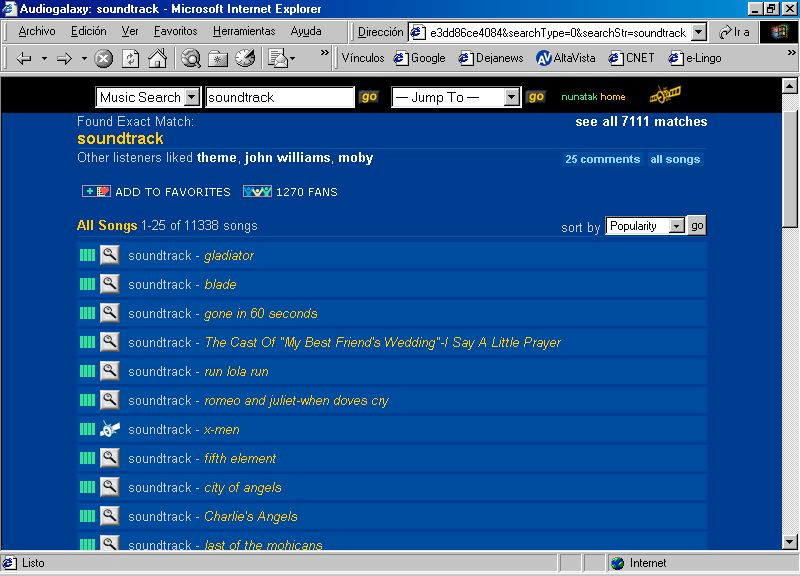
\includegraphics[width=1\textwidth]{pictures/cap1/audiogalaxy}
\caption{Interface do programa Audiogalaxy de compartilhamento de músicas.}
\label{fig:audiogalaxy}
\end{figure}


Com essa pesquisa de repertório adquirido na internet, através da nova cultura de dádiva que se estabelecia, acabei assumindo a posição de DJ em alguns happy hours quando em 2001 participei pela primeira vez da gestão do Gfau, o grêmio de estudantes da FAU, junto à chapa ``Estúdio 5''. Foi nesse ano também que surgiu um interesse especial pelo design de interfaces. Na época começaram a ser populares experimentos interativos\footnote{\cite{Pindado2005}} de Yougop\footnote{\url{http://yugop.com/} está hoje fora do ar} e John Maeda (1995)\footnote{O site antigo com as animações online ainda está no ar até hoje na url:\url{https://maedastudio.com/oldindex.php}}. As animações eram baseadas em flash, um sistema de propriedade da empresa Adobe, que fornecia um editor -- pago -- e um leitor -- gratuito para dar suporte a aplicativos online. Muitos foram utilizados pela indústria de jogos, mas também pela indústria do entretenimento. Por permitir a manipulação de arquivos multimídia diretamente no navegador, \emph{flash} foi a tecnologia empregada também na primeira versão do youtube. 


 Por volta de 2001, comecei a fazer algumas experiências com animações em \emph{Flash}, entre elas o site para a ``Expofau 2001'' em parcerceria com Ciro Miguel.\footnote{Em 2001 a Expofau foi excepcionalmente grande e contou com a participação de mais de uma centena de artistas.}, mas ainda era para a mídia impressa que dedicava mais atenção e força de trabalho. Fiz uma iniciação científica bem técnica em design gráfico, investigando legibilidade de texto  e me engajei em diversas comissões do Gfau, grupos de extensão e organizações estudantis – Revista Caramelo, Jornal 1:100, Labhab Gfau, Grupo Anita Garibaldi, Revista Contravento e da fundação da Negação da Negação. Pudemos experimentar com várias técnicas de composição gráfica digitais e analógicas por ter acesso a um laboratório de produção gráfica\footnote{O LPG era coordenado pelo arquiteto Tadeu Maia e foi bastante receptivo ao desenvolvimento da nossa produção. O laboratório tinha equipamentos de serigrafia, impressão digital, tipografia, impressão offset e encadernação e fotolito.} e uma cota mensal de uso de xérox. Foi uma época de extensa produção estudantil, do surgimento da ``Fau Paralela'', ``expressão dessa consciência de que a escola e o aprendizado estão em grande parte fora da instituição, do curricular'', como aponta Ana Carolina Ribeiro (2006) no seu TTG ``trans Forma Ação'', que analisa a produção gráfica da FAU na época \footnote{\cite{Ribeiro2006}}. 

\begin{figure}

\includegraphics[width=1\textwidth]{pictures/cap1/manualdosbixos}
\caption{Manual dos bixos da chapa Concreto Armado, 2003.}
\legend{Fonte: Acervo da autora.}
\label{fig:bichos}
\end{figure}

Esses processos de produção que me envolvi na época eram sobretudo coletivos, então experimentávamos com técnicas como stêncil, e fotomontagens, que permitiam o envolvimento de bastante gente no processo\footnote{Isso foi uma conclusão que chegamos na época em uma das reuniões da comissão da editora do Gfau, onde discutimos a dificuldade de se trabalhar processos coletivos de composição gráfica utilizando o computador.}. Uma série de produções foram desenvolvidas com essas técnicas, como o manual dos bichos de 2003 (Figura \ref{fig:bichos}) que explorava uma estética de despojamento gráfico. Nessa época, comecei a desenvolver as primeiras pesquisas em composição gráfica modular, que chamava de ``Concretismo Tosco'', pela inspiração concreta e a precariedade no acabamento, como os apresentados na figura \ref{fig:tosconcreto}. Essa defesa de uma certa precariedade era uma influência do pensamento do arquiteto Sérgio Ferro, que defendia a manutenção do erro como um marca do trabalho na obra de arte \footnote{\cite{FerroSergio2002}} ou da idéia de ``precariedade radical'' de Lina Bo Bardi. No projeto do teatro oficina, Lina partiu da precariedade em que estava o local e da escassez de recursos como recurso estético.  \cite{Macedo2015}. 

Do ambiente da FAU, também surgiram muitas referências, sobretudo de estética brutalista. Da arquitetura moderna e do brutalismo de Vilanova Artigas, os concretistas russos como El Lissitsky e Rodchenko e brasileiros como Sacilotto, Athos Bulcão e Lygia Pape, Augusto de Campos, Haroldo de Campos e Décio Pignatari. Um princípio que levávamos a cabo era o da antropofagia oswaldiana.  ``A alegria é a prova dos nove'', apontava Oswald de Andrade no ``Manifesto Antropófago''\footnote{\cite{Andrade1928}}. Procuramos seguir muitos princípios da antropofagia como base, como a devoração e deglutição dessas referências no nosso trabalho prático coletivo. Por volta de 2005, com as atividades do grupo de intervenção teatral\footnote{Que posteriormente se tornou o Coro de Carcarás.} comecei a ter um envolviento mais direto com práticas musicais, através da voz, da alfaia e do xequerê. 

%Desde meus primeiros envolvimentos com música e performance no Coro de Carcarás, por volta de 2005, a influência da antropofagia Oswaldiana foi bastante significativa.

%Aqui, 

%não queremos trazer essas referências como inspiração ou nostalgia, mas como apontamentos para pensar possibilidades estéticas. Como os princípios de racionalidade,  e sobretudo uma postura anti-decorativa, anti-ornamental e de procurar um mínimo de elementos necessários.

\begin{figure}

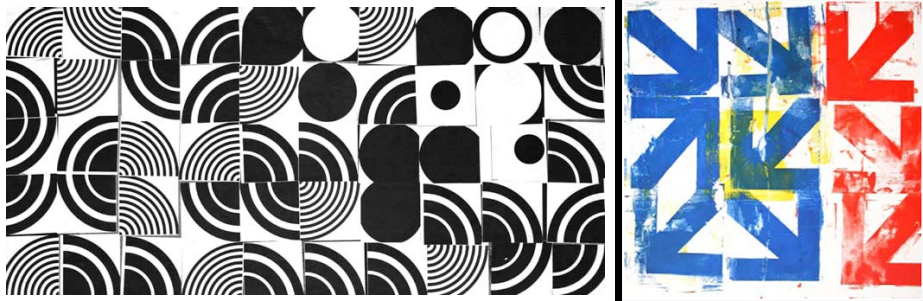
\includegraphics[width=1\textwidth]{pictures/cap1/tosconcreto}
\caption{Painéis tosconconcretos montados na FAU.}
\legend{Fonte: \cite{Ribeiro2006}.}
\label{fig:tosconcreto}
\end{figure}

Em 2005, o professor belga Etienne Delacroix veio ao Brasil oferecer a disciplina ``Oficina de Arte e Programação'' na Escola de Engenharia Politécnica (Poli), que tive oportunidade de cursar como optativa. Ele instalou numa sala o Atelier Labs, uma mistura de laboratório e atelier, onde os alunos poderiam desenvolver projetos de seu interesse, relacionados com os temas que o professor nos apresentou, que iam de reciclagem de computadores, instrumentos musicais DIY, robôs, software livre e programação para web. O Atelier Labs acabou sendo um  centro difusor de cultura livre em São Paulo. Colaborou na formação de uma rede de ativistas em cultura digital que atuam até hoje em diversas cidades do Brasil. A proposta pedagógica do professor era de fazer com que os alunos conseguissem se embrenhar na ``caixa preta'', desdevendando o funcionamento dos computadores e das lógicas de programação \footnote{\cite{Delacroix2009}}, para isso, fazia uso de computadores velhos que eram desmontados e re-configurados em torres, com seus compontentes à mostra. O Atelier Labs (Figuras \ref{fig:eti} e \ref{fig:eti2}) também se convertia em uma estrutura móvel que podia ser montado em lugares diferentes, acompanhando o professor onde ele precisasse como em oficinas em escolas públicas e eventos como o Fórum Mundial de Software Livre ou a Campus Party.

\begin{figure}

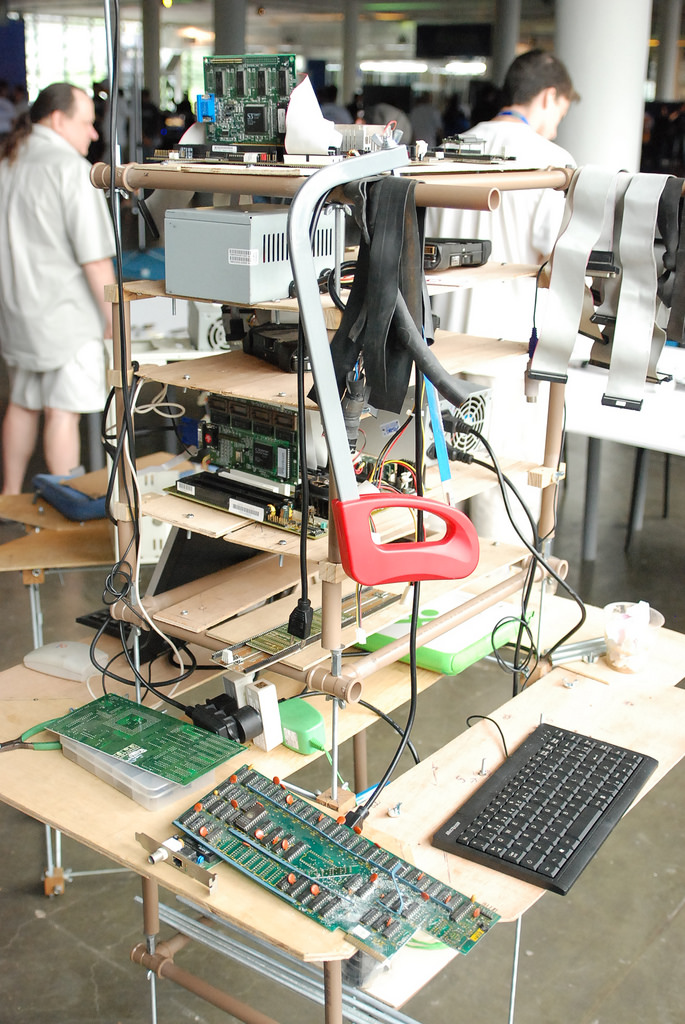
\includegraphics[width=0.5\textwidth]{pictures/cap1/eti1}
\caption{Ateliê móvel de Ethienne Delacroix.}
\legend{Fonte: Campus Party Brasil, 2008.}
\label{fig:eti}
\end{figure}

\begin{figure}

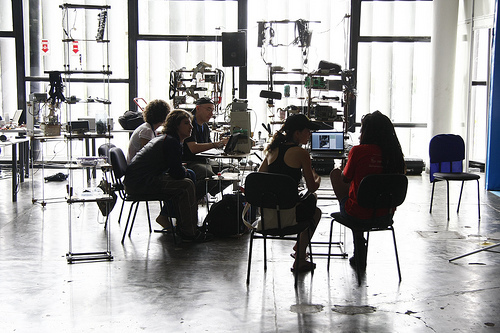
\includegraphics[width=1\textwidth]{pictures/cap1/eti2}
\caption{Aula da disciplina Ofina de Arte e programação, na Escola Politécnica.}
\legend{Foto: Fernando Cavalcanti.}
\label{fig:eti2}
\end{figure}

O professor Ethienne foi que também quem me colocou em um contato mais próximo com discussões a respeito do que se chama de ``Cultura Livre''. A cultura livre é defendida por uma comunidade de pensadores, programadores e artistas, como Lawrence Lessig (2004), e a iniciativa Creative Commons, Richard Stallman e a comunidade do software livre, e mesmo Alexandra Elbakyan com o Sci Hub que desafia constantemente a propriedade da informação, \footnote{(Barok et al, 2015)} entre vários outros que têm constantemente limitado por diversas práticas culturais libertárias. Barbrook (\citeyear{Barbrook2009}), aponta o movimento do software livre como uma oposição às políticas das mega coorporações como a Microsoft:

\begin{citacao}
Durante a explosão ponto com do final dos anos 1990, Richard Stallman – um cientista da computação do MIT e guru da Fundação do Software Livre (Free Software Foundation) – resistiu firmemente à pressa em comercializar a Internet. Fiel à visão de Licklider, ele defendeu a ética hacker de esforço coletivo e investigação aberta. Da perspectiva dos laboratórios de pesquisa universitários, os programas de computador proprietários possuíam um defeito de fábrica intrínseco: restrições de propriedade intelectual. Dentro da economia da dádiva acadêmica, programadores eram encorajados a compartilhar, apropriar e melhorar o trabalho de todos. Em oposição, a Microsoft e outras empresas comerciais guardavam enciumadas os segredos de seus códigos-fonte. Os usuários de computador foram impedidos de tornarem-se, além de consumidores, produtores de programas.\footnote{\cite[367]{Barbrook2009}}
\end{citacao}

A ideologia por trás do Atellier Labs, tinha muito dessa idéia de cultura livre. Para ele, aprender programação na prática seria uma atividade libertadora, no sentido de produzir agentes capaz de recriar a partir de materiais obsoletos, reprogramar sistemas e propor novos códigos. Essa ideologia é compartilhada também por muitos outros pesquisadores que trabalham com a ideia de software livre, como apontam os autores do projeto Música Móvel:

\begin{citacao}
Como ideologia, é preciso pensar o que o histórico do uso de softwares livres está sempre de alguma forma relacionado com contextos de colaboração bastante politizados quanto à problematização da tecnofilia voraz que alimenta uma efêmera obsolescência dos dispositivos digitais e seus padrões industriais concorrentes. A manutenção e compartilhamento do legado destes projetos abertos em licenças livres gera uma ecologia menos amarrada na competição predatória dos padrões em jogo e torna o processo mais objetivo quanto uma busca pragmática de conhecimento e construção de um rede de interessados na continuidade destes legados.\footnote{\cite{Rohde2014}}
\end{citacao}



\section{Da rede à música}
O envolvimento nas atividades políticas estudantis, levou à participação em uma série de atividades musicais, inicialmente com a organização de festas, depois como percussionista no grupo Urbando, um núcleo do Gfau que atuava em festas e manifestações estudantis e posteriormente em atividades de livre improvisação que aconteciam às quintas feiras no gramado da FAU, o Som de Quinta. Esse engajamento me levou a uma paixão pela música como atividade prática e cotidiana, não mais somente como ouvinte. Barthes (\citeyear{Barthes1978}) aponta para uma ideia de ``música prática'', que é um tipo de música que é mais para ser executada do que para ser ouvida, ligada a uma tradição musical mais ritualística e que foi um pouco abandonada pela ``Música'' ocidental. 


Após a experiência com o professor Ethienne, surgiu a vontade de explorar a rede como suporte, inicialmente como meio de divulgação de uma cena experimental que estava acontecendo naquele momento. Aluguei um provedor de internet, onde começamos a organizar um site para colocar materiais meus e de colegas -- o Finetanks.com. \footnote{No começo do site, tínhamos uma seção de ilustrações, minhas em HTML e de Guilherme Garbato, minha pesquisa de iniciação científica, ``Legibilidade e Evolução das Mídias'', desenvolvida entre 2000 e 2001,e alguns primeiros experimentos em arte interativa: painéis modulares randômicos programados em php inspirados nas obras de Athos Bulcão.}
   
Os primeiros projetos musicais hospedados no Finetanks foram duas bandas punks, ``Os Otávios'' e ``Desprezíveis'', Cabeça de Câncer e Protomúsica, meu projeto solo de música eletrônica. Os``Os Otávios'' eram uma banda punk com inspiração semiótica, que tocava em círculos ligados ao movimento estudantil na época\footnote{Teve diversas formações que incluíram: Reginaldo Yasuoka, Vítor Serra (Walther Vítor), Daniel Ávila, Francisco França, Bodão Bode, Guilherme Cenoura e Ariane Stolfi} e Os ``Desprezíveis'' eram uma banda punk de perifeira, cujas músicas do álbum ``Eu não sei nada o que é saber mais do que você'' não ultrapassam 28 segundos de duração\footnote{``Desprezíveis'' era formada por Rogê, Leandro e Gas.}. ``Cabeça de Câncer'' era um trio de improvisação musical que eu formava com Guilherme Garbato e Fernando Bizarri e Protomúsica era meu projeto solo de música eletrônica. Com o tempo, foram anexados outros projetos como o JazzMetak, projeto de improvisação livre de Rômulo Alexis, Francisco França, Rogério Gobet e TH; Freetools, de free jazz e Organograma, projeto de música eletrônica de Fernando Bizarri.

Tinha começado a produzir música eletrônica em um software que se chamava Jeskola Buzz, um software gratuito meio obscuro, usado por alguns artistas da cena eletrônica, principalmente em alguns circuitos ligados ao IDM (Intelligent Dance Music). No Brasil, o músico Retrigger (Raul Duarte), e o Organograma usavam-no como base para produção musical. O software funcionava uma plataforma aberta -- embora não \emph{open-source} -- para a criação de instrumentos e disponibilizava uma ampla gama de sintetizadores e efeitos de áudio. O Buzz tinha uma interface bastante peculiar, que alternava entre três espaços:

\begin{itemize}
\item Um para estabelecer rotas de comunicação entre de processamentos de sinais digitais (DSP) (Figura \ref{fig:buzz1});
\item Um para desenhar padrões para os instrumentos e efeitos, que lembrava um cartão perfurado. Os parâmetros eram definidos em linguagem Hexadecimal e as notas no sistema de notação americano (Ex: C-3, etc) (Figura \ref{fig:buzz});
\item Uma linha do tempo, onde se podia distribuir os padrões desenhado ao longo do tempo (Figura \ref{fig:buzz3});
\end{itemize}

\begin{figure}

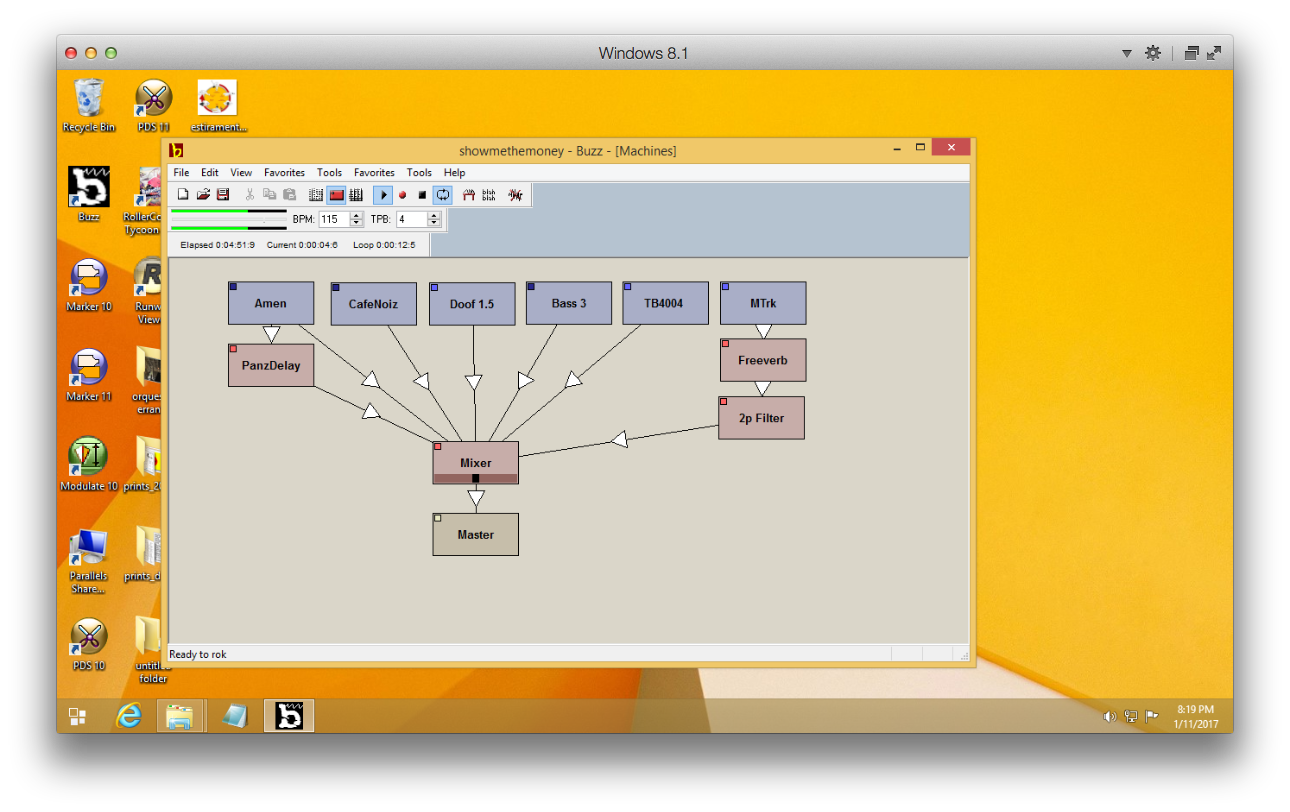
\includegraphics[width=0.8\textwidth]{pictures/cap1/buzz1}
\caption{Interface do programa Buzz, mapa de conecções.}
\label{fig:buzz1}
\end{figure}

\begin{figure}

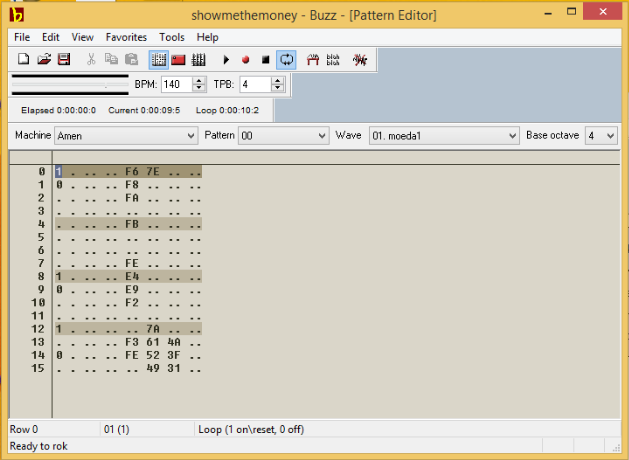
\includegraphics[width=0.8\textwidth]{pictures/cap1/buzz}
\caption{Interface do programa Buzz, editor de padrões}
\label{fig:buzz}
\end{figure}

\begin{figure}

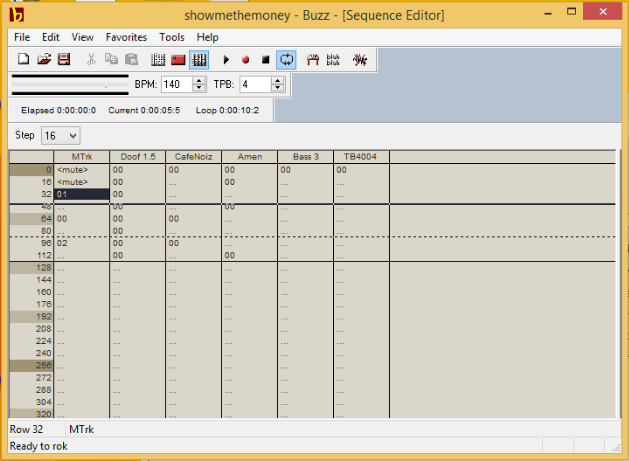
\includegraphics[width=0.8\textwidth]{pictures/cap1/buzz3}
\caption{Interface do programa Buzz, editor de linha do tempo.}
\legend{Fonte: screenshot da autora}
\label{fig:buzz3}
\end{figure}

Com ele, comecei a desenvolver uma série de conhecimentos práticos em métodos de síntese e processamento de áudio, que organizei em experimentos sonoros metalinguísticos, chamados de Protomúsica. Metalinguísticos porque o próprio processo de composição levava em conta uma experimentação com os instrumentos e os materiais musicais, por exemplo:
Estudo de harmonia e dissonância num ré.\footnote{Disponível em: \url{http://finetanks.com/records/2005_2010/protomusica/estudo\%20de\%20harmonia\%20e\%20dissonancia\%20num\%20re.mp3}}, explora as possibilidades de intervalos musicais em um sintetizador aditivo;
Dodecafunk, uma batida de funk carioca com uma melodia que segue regras de composição dodecafônicas.\footnote{Disponível em: \url{http://finetanks.com/records/2005_2010/protomusica/dodecafunk.mp3}}
Percussiva, explora as possibilidades de variação de timbre a partir de um padrão rítmico de apenas uma nota no sintetizador percussive FM.\footnote{Disponível em: \url{http://finetanks.com/records/2005_2010/protomusica/percussiva.mp3}}



\begin{figure}

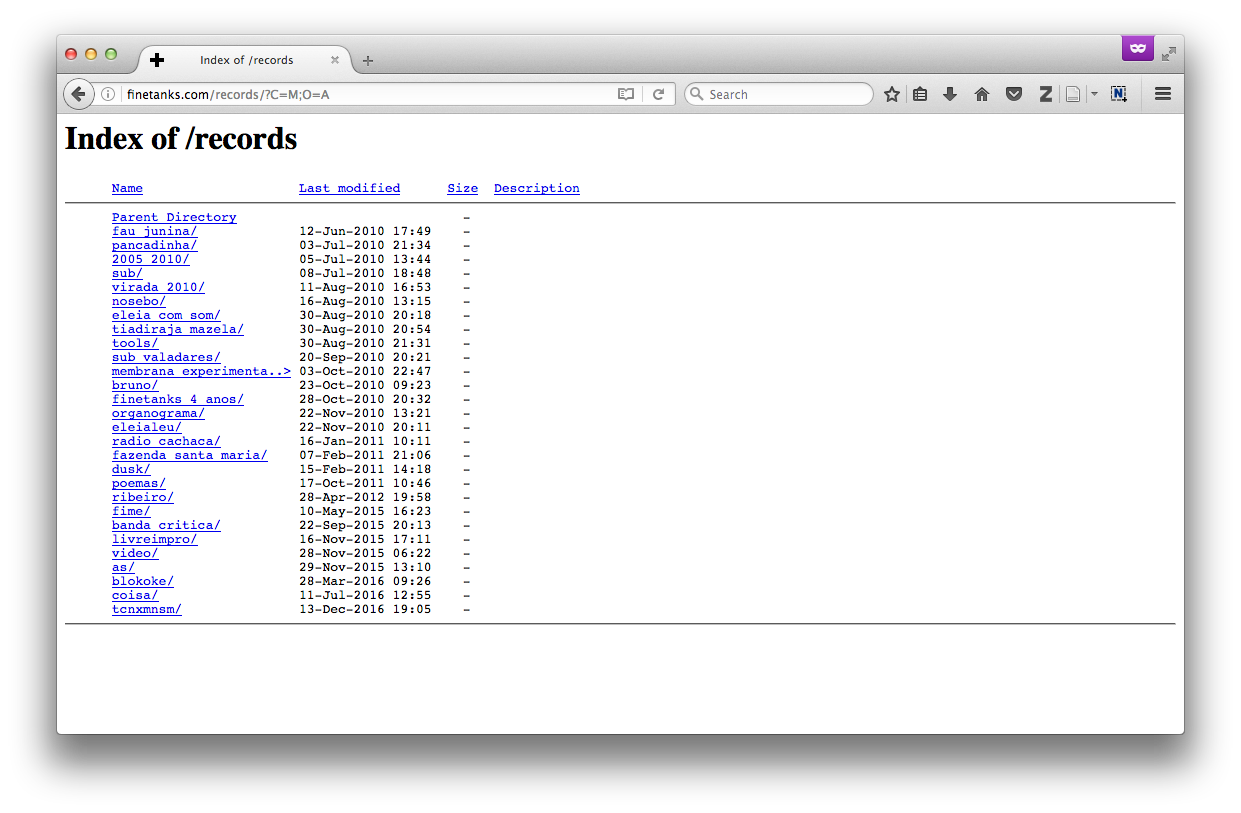
\includegraphics[width=1\textwidth]{pictures/cap1/finetanksrecords}
\caption{Finetanks.com.}
\legend{Fonte: screenshot da autora}
\label{fig:finetanks}
\end{figure}




\subsection{Cultura Digital}

Logo após terminar a graduação, em 2006, comecei a trabalhar como pesquisadora na equipe do Hacklab, um grupo de desenvolvedores web que atuava em São Paulo financiados pelo projeto Cultura Digital, do Ministério da Cultura (MinC), para fornecer recursos para os pontos de cultura, que chegavam a 1000 unidades em 2006\footnote{\cite[6]{Lima2009}}. Os pontos de cultura foram criados em 2004 na gestão de Gilberto Gil do MinC, para fomentar espaços culturais independentes em todas as regiões do país, ou segundo ele:
\begin{citacao}

``Para fazer uma espécie de do-in antropológico, massageando pontos vitais, mas momentaneamente desprezados ou adormecidos, do corpo cultural do País. Enfim, para avivar o velho e atiçar o novo.''\footnote{\cite{GilbertoGil2003}} 
\end{citacao}

Entre os projetos que estavam sendo desenvolvidos pela equipe do Hacklab estava o \url{Estudiolivre.org}, que tinha como objetivo ``a formação de espaços reais e virtuais que estimulem e permitam a produção, a distribuição e o desenvolvimento de meios de comunicação e de informação livres''\footnote{\cite[12]{Lima2009}} e oferecia ferramentas para download e compartilhamento de arquivos de imagem, som e vídeo, além de manuais, fóruns e páginas pessoais, e é considerado um projeto pioneiro na cultura digital no Brasil.  


O trabalho no Hacklab me colocou em contato com grupos diferentes de pessoas atuantes nos circuitos de produção de cultura livre, em diferentes redes, como a Metareciclagem, Estudiolivre, Coletivo Coro, CMI e a Rede Saravá. Com o fim do projeto, me aproximei da rede Submidialogias, que foi criada por volta de 2005 para fomentar e debater política e cultura digital no Brasil agregava cerca de 200 ativistas de todo o país, uma rede auto organizada não hieráquica que se organizava por uma lista de e-mails e tinha como base princípios de livre cooperação e democratização de conteúdos\footnote{\cite{Brunet}}. A rede também organizava encontros anuais que funcionavam em um processo de imersão coletiva, como descreve Fabiane Borges (\citeyear{FabianeMoraesBorges2010}):

\begin{citacao}
Imersão é uma disponibilidade, um engolfamento, um mergulho e, se bobear, um afogamento. Trata-se de um modo de perceber/sentir um determinado espaço/tempo casual ou produzido voluntariamente. Utilizamos a palavra imersão no rastro do conceito de Deleuze: acontecimento, extraindo de seus entremeios, uma viva ideia de ativismo, pois estamos falando de uma disposição individual/coletiva para criação de situações de resistência aos paradigmas ambientais-político-sociais da contemporaneidade.

Uma imersão coletiva é circunstância rítmica com atuação incisiva sobre os corpos dispostos a vivenciarem a experiência;
\end{citacao}
 
Coletivos participantes desta rede tinham como característica o uso de diversas mídias como suporte e abordavam uma multiplicidade de temas, para práticas que se enquadravam principalmente nas tradições da ``arte urbana'' e das ``práticas artísticas coletivas'', como aponta Tkatschuk (\citeyear{Tkatschuk2011}) no seu artigo sobre a Orquestra Organismo, um dos coletivos que atuava na rede. O grupo reunía os músicos e programadores Lúcio Araújo, Guilherme Soares, Octávio Camargo, Simone Bittencourt e outros colaboradores que interagissem com o processo, que buscava criar ``um fluxo artístico interdisciplinar e colaborativo, agenciador de inúmeras ações''\footnote{ARAÚJO, 2007 in \cite{Tkatschuk2011}}. Essas ações envolviam encontros, confeção de instrumentos novos, como o ``Toscolão'', um violão híbrido que condensava sistemas de captação, processamento de áudio e distorções, grafismos, colagens, mapeamentes e ``rituais relacionais'', e assinava seus projetos por meio de uma autoria coletiva. 



\subsection{Records}
Em 2007 e 2008, pude participar de dois desses encontros imersivos da rede Submidialogias, em Arraial D'Ajuda e na Ilha de Valadares. Havia comprado um gravador estéreo portátil e comecei a fazer algumas gravações em campo. Nesses encontros, participamos de uma série de processos imersivos de produção musical, e gravei uma quantidade considerável deles, como \emph{jams} e processos um tanto catárticos de improvisação e composição coletiva, em conjunto com Felipe Ribeiro, Jerônimo Barbosa, Fabiane Borges, Ricardo Brasileiro, Glerm Soares, Kaloan Menochite, Giuliano Obicci, Pan\&tone, e outros. Tocávamos com o que estivesse disponível na hora: voz, patches de Pd, violão de duas cordas, gambiarras eletrônicas e batuques. \footnote{Esses processos eram às vezes sessões de improvisação musical, mas muitas vezes direcionadas para processos de composição musical em tempo real, onde fazíamos também canções, sobre coisas que pensávamos ou sentíamos, ou sobre acontecimentos e fatos marcantes do momento, por exemplo: ``Ganhei um edital, eu tenho capital, pro meu programa social'', cantando sobre o processo de ganhar o edital Rumos da Petrobrás, que financiou os festivais; ou ``A gripe B é uma balela'', sobre uma gripe que se anunciava entre os participantes do Sub Valadares, ou ``Rasta Burocrata'', sobre um colega rastafari que estava tendo que assumir tarefas burocráticas na organização.}.


Passei então a editar o material gravado e transformei o Finetanks em uma pequena gravadora independente. Não havia suporte para áudio ainda na linguagem HTML, e para construir as páginas dos projetos era preciso inserir \emph{iframes} com o endereço dos arquivos originais, processo que era relativamente trabalhoso e bastante artesanal, então, em 2010 o site foi transformado em um repositório, sem páginas em HTML para cada projeto, e o material passou a ser organizado em em subpastas, com os links diretos para os arquivos em mp3, sem nenhuma informação extra além do nome do arquivo, data de modificação e tamanho. 


\begin{figure}

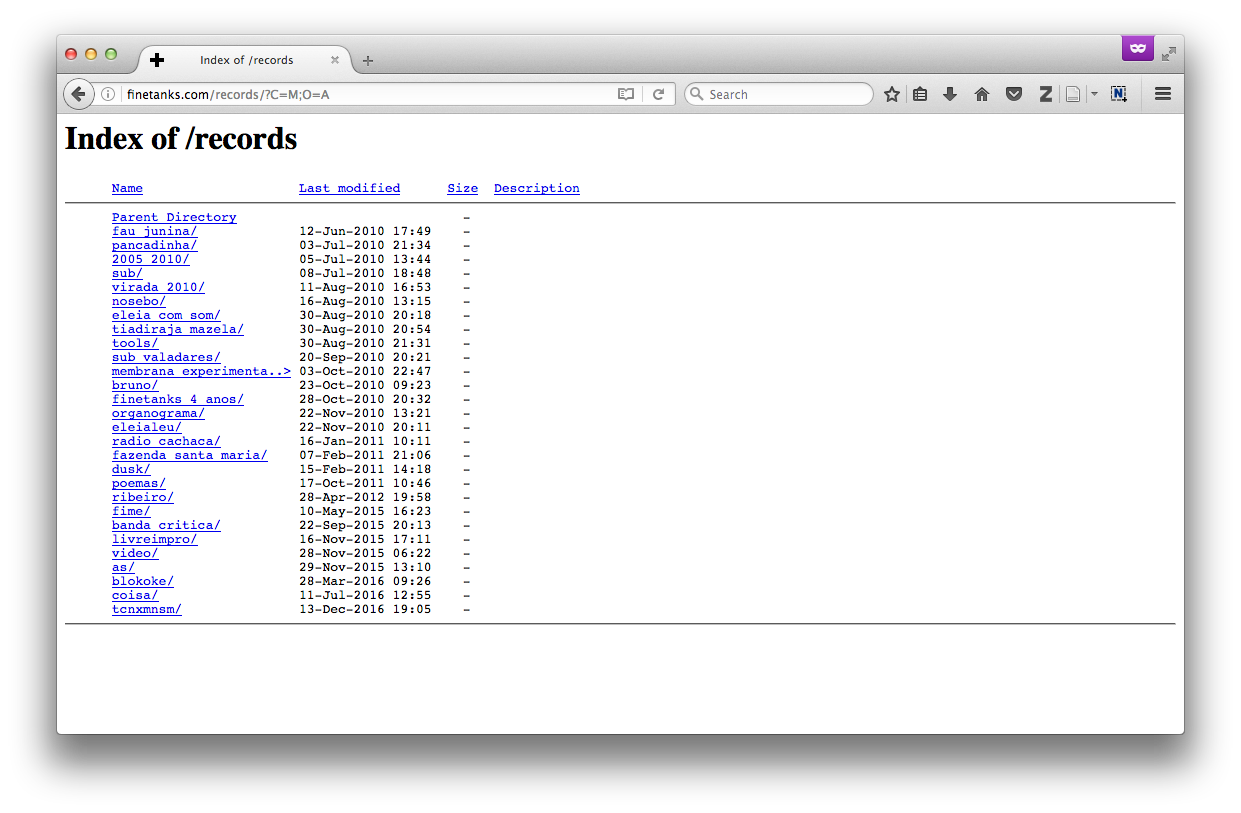
\includegraphics[width=1\textwidth]{pictures/cap1/finetanksrecords}
\caption{Interface do repositório \url{http://finetanks/records}.}
\label{fig:finetanksrecords}
\legend{Screenshot da autora, 6 de janeiro de 2017.}
\end{figure}


\begin{figure}

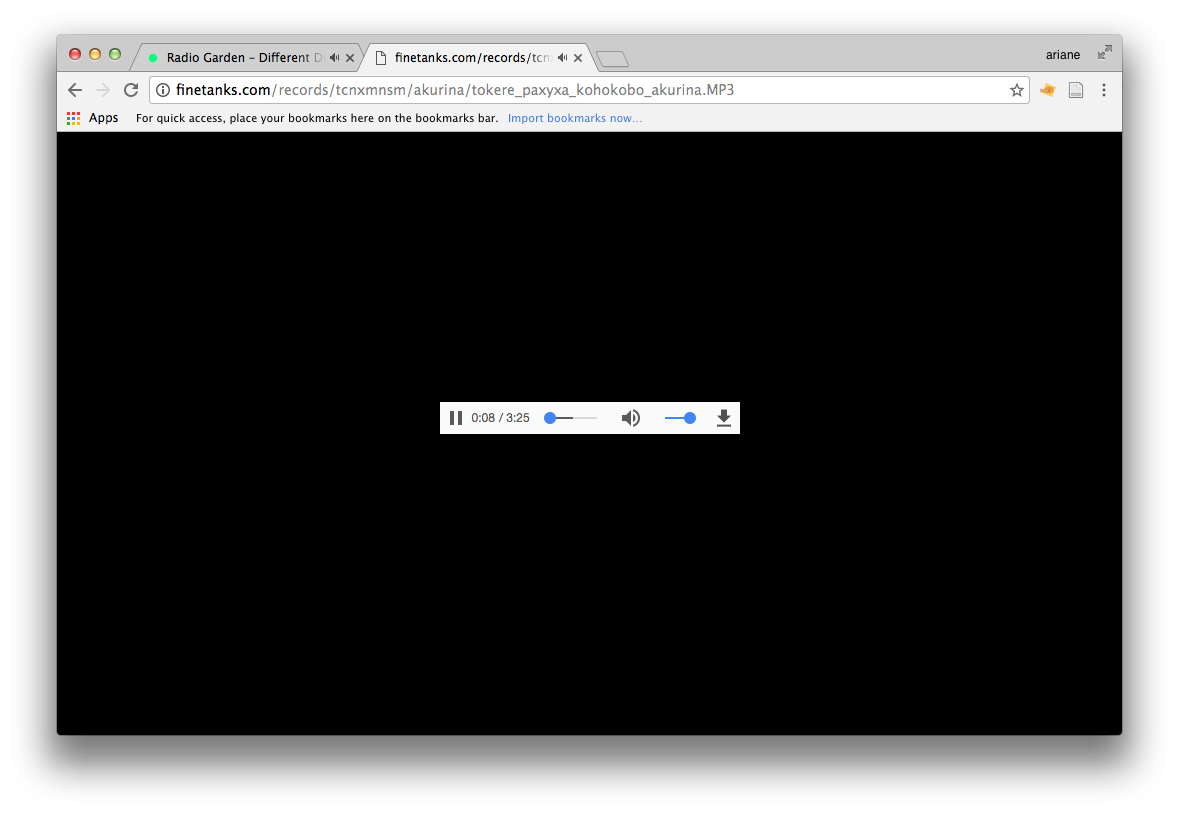
\includegraphics[width=1\textwidth]{pictures/cap1/finetanksmp3}
\caption{Os arquivos de áudio são acessados pela interface padrão do navegador.}
\label{fig:finetanksmp3}
\legend{Screenshot da autora, 6 de janeiro de 2017.}
\end{figure}

Apesar de uma aparência até meio tosca, a estrutura é bastante funcional, pois permite um rápido compartilhamento e acesso, com muito pouco uso de dados, além de ser compatível com a imensa maioria dos sistemas e dispositivos. É, de uma certa forma, como a estrutura exposta de um edifício brutalista. Surpreendentemente, quando removemos as páginas HTML, a audiência do site aumentou bastante, chegando a 2000 acessos diários em 2011 e até hoje ainda contando com uma média de 600 acesso por dia. 

Desde as minhas primeiras pesquisas com código HTML e CSS, procurei experimentar com uma idéia estética de ``brutalismo digital''. Essa idéia é conhecida como uma tendência estética no mercado de web design\footnote{\cite{Hill2017}}, mas não é muito elaborada teoricamente ainda. Nossa idéia era de que assim como na arquitetura, seria possível pensar em interfaces brutalistas, onde não houvessem, por exemplo, elementos desnecessários ou decorativos no design. No repositório do Finetanks, essa idéia foi levada ao extremo, com páginas sem páginas, onde se organizam somente os arquivos originais, da maneira em que o navegador os reconhece.  


	Entre 2010 e 2011 editei e postei no ``Finetanks'' uma série de músicas próprias e de terceiros, que estão organizadas nas diversas pastas do repositório\footnote{ Por exemplo, as canções compstas coletivamente no festival de Submidialogias de Arraial D'Ajuda e do Ruidocracia no Rio de janeiro (\/sub\/); das apresentações com o Coletivo 24h do projeto Cromocinética, e de Ricardo Carioba, na Virada Cultural no MIS (virada\_2010\/); apresentações musicais no sebo Elea com Gabriel Kerhart, Rômulo Alexis e Felipe Ribeiro (nosebo\/); arquivos da banda (tiadiraja\_mazela\/) de Kaloan Menochite e Pilantropov Pausanias, gravações do ritual final de encerramento do festival de Submidialogias de Paranaguá, com participação de Glerm Soares, Felipe Ribeiro, Fabiane Borges, Roger Bagé, Lucida Sans e membros da comunidade caiçara da ilha (\/sub\_valadares\/); jam sessions do grupo Membrana Experimental Fiat Lux, coordenados por Rômulo Alexis e Leila Monsegur (membrana\_experimental\_fiatlux\/); gravações de Bruno Araújo (Walter Rego), em seções de improvisações de rap no Gfau (bruno\/); diversas gravações dos encontros Eleia leu,  de leituras poéticas organizado por Gabriel Kerhart, na biblioteca Alceu Amoroso Lima e na galeria Bordô, que inclui participações de Amélia Monteiro, Ana Gold, Bruno Schiavo, Gabriel Kolyniak, Diego Sampaio, Marcelo Maccaferri, Felipe Ribeiro entre outros, (\/eleialeu\/) até as gravações feitas na Fazenda Santa Maria, de Thereza Amaral, que incluiu uma experiência lisérgica pesada que que envolveu um certo grau de incorporação, que batizamos de Exu na Cozinha (\/fazenda\_santa\_maria\/), uma experiência que foi bastante catártica e de certa forma amedrontadora. }.Interrompi as atividades do selo por um tempo após ter o gravador digital furtado depois de uma apresentação solo realizada no 2o Festival \#Dis Experimental, tendo retomado somente em 2015, depois de iniciar as pesquisas neste doutorado. A essa altura, também já havia uma série de ferramentas para publicação online de conteúdo, como SoundCloud e Youtube, onde os próprios artistas podem alimentar com conteúdo, e a gravadora já não era mais tão necessária.





\subsection{Pure Data}

A experiência prática junto ao Hacklab em software livre me levou propor ao recém inaugurado Lab-C, no Centro Cultural da Juventude da Prefeitura Municipal de São Paulo (PMSP), que procurando desenvolver a ``produção cultural integrada às práticas de difusão do conhecimento a partir do uso de softwares livres'', oferecia oficinas práticas de ``metareciclagem, áudio, vídeo, rádio e gráfico''\footnote{\cite{PMSP2008}}, oficinas de design gráfico baseadas em software livre. Ministrei uma oficina onde procurava apresentar um certo repertório da história do design como El Lissitzky, Alexandr Rodchenko, Josef Muller Brockmann, Paul Rand, Aluízio Magalhães, Rogério Duarte e César Vilela, alguns conceitos teóricos de Gestalt e Semiótica, e questões técnicas como tipografia e diagramação, realizando exercícios práticos de acordo com os interesses dos grupos majoritariamente de jovens que frequentavam a oficina. Nesse período, pude participar também participar da oficina ``DESIGN E INTERAÇÃO SONORA'', Ministrado por Giuliano Obici:
\begin{citacao}
Curso de programação e invenção musical com o intuito de apresentar conhecimentos técnicos e teóricos sobre o áudio no meio digital e de alguns dispositivos como microfone, interfaces, controlador MIDI, sensores e circuitos envolvendo o ambiente de programação Pure Data (PD). \footnote{\cite{PMSP2008}}
\end{citacao}

O ambiente de programação PD, assim como o Max, oferece a possibilidade de programar processos de síntese e controle de áudio vídeo e dados, em uma interface gráfica que interliga objetos representados por caixas de texto através de linhas em uma tela, possibilitando ao programador controlar fluxos de informação em um esquema de hierarquias semelhante aos diagramas de arquitetura de informação. 

Essa possibilidade de programação visual foi bastante estimulante, pois a linguagem de blocos interligados que sua interface oferecia era um tanto semelhante à do Buzz, e era mais fácil de compreender do que a programação por escrito, pela visualidade da informação. Ao mesmo tempo, a lógica era totalmente diferente; enquanto o Buzz é uma ferramenta de composição linear, com linha do tempo e instrumentos pré-programado, Pd é um ambiente de programação complexo, cuja interface, como analisamos no artigo ``Graphic Interfaces for Computer Music: Two Models'', não comunica muito ao usuário o que se é possível fazer \footnote{\cite{Stolfi2016}}. 
Em 2009 aconteceu uma conferência internacional de PD em São Paulo, onde pude entrar em contato com uma série de trabalhos inovadores em arte sonora e música experimental, como os trabalhos dos duos CHDH de Cyrile Henry e Nicolas Montgermont (Figura \ref{fig:chdh}), que tocam um sintetizador audiovisual com correspondência entre os processos de síntese sonora e de movimento e Hp-Process de Philippe Boisnard e Hortense Gauthier (Figura \ref{fig:hp}), onde a performer nua e grávida era transposta para dentro de um universo poético tipográfico construído em 3 dimensões e manipulado em tempo real através de sensores adaptados de kinetics e interface em Pure Data. 

\begin{figure}

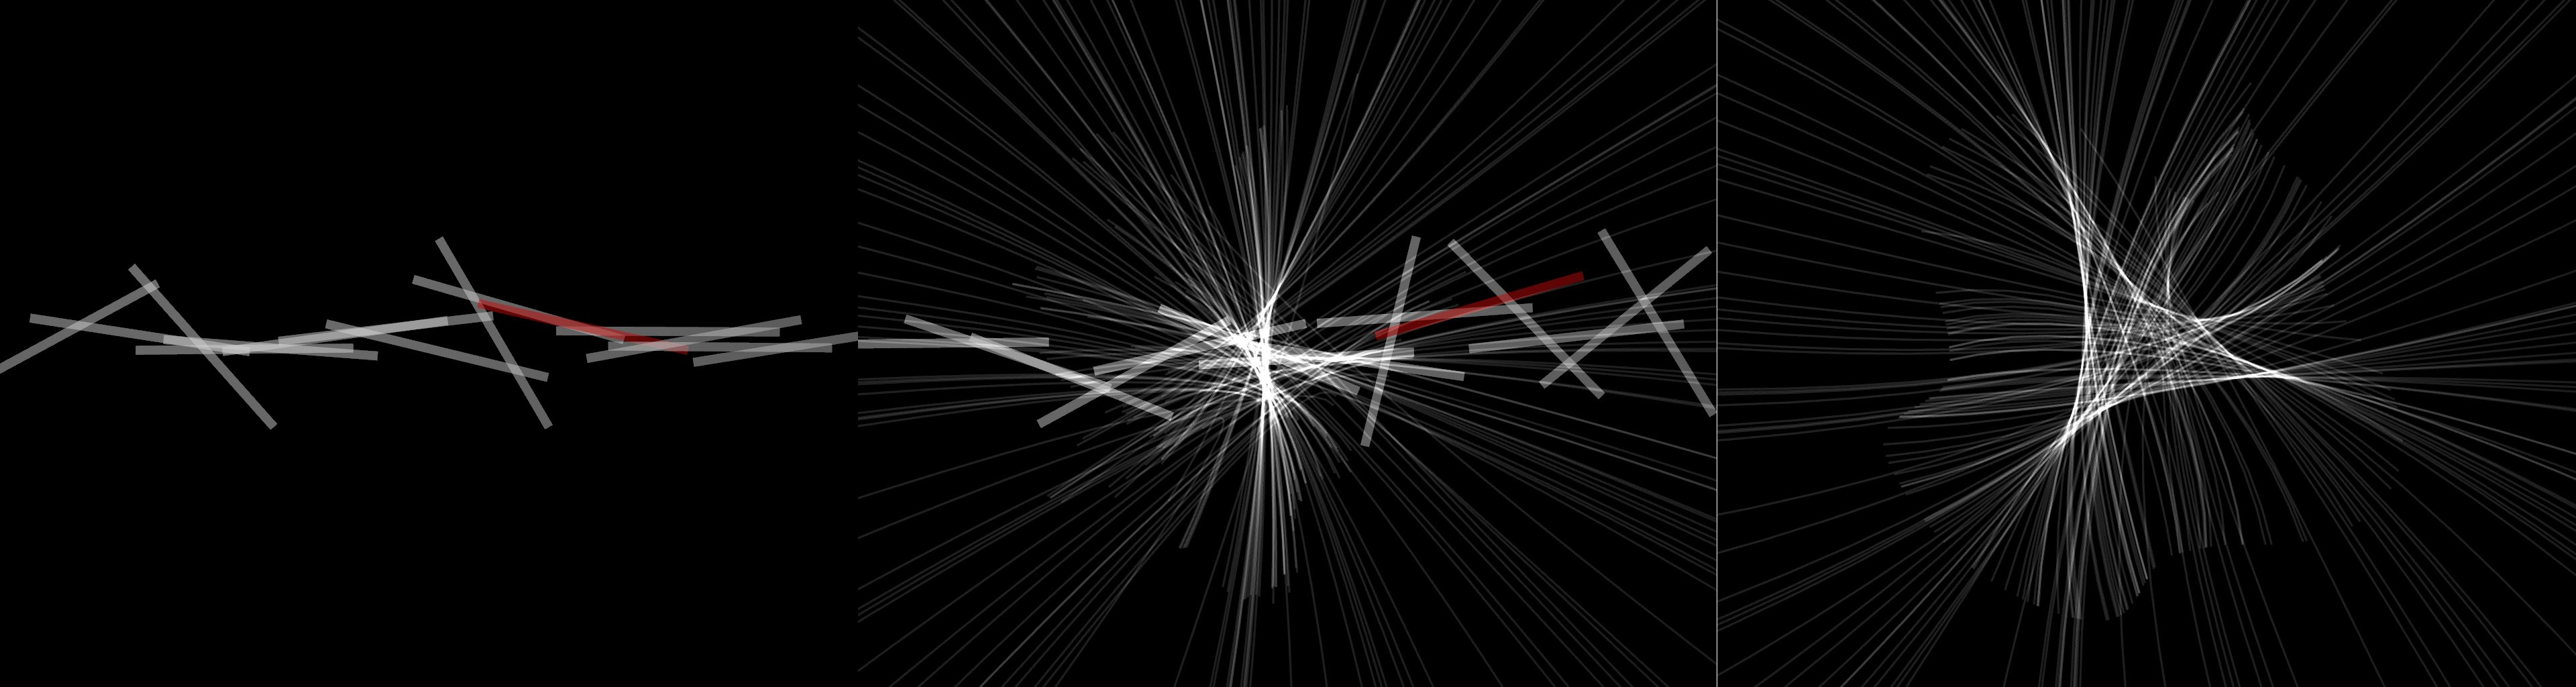
\includegraphics[width=1\textwidth]{pictures/cap1/CHDH}
\caption{Detalhes da performance Eggregore, do grupo CHDH apresentada na PdCon em 2009.}
\label{fig:chdh}
\legend{Fonte: \url{http://chdh.net/egregore.php}}
\end{figure}

\begin{figure}

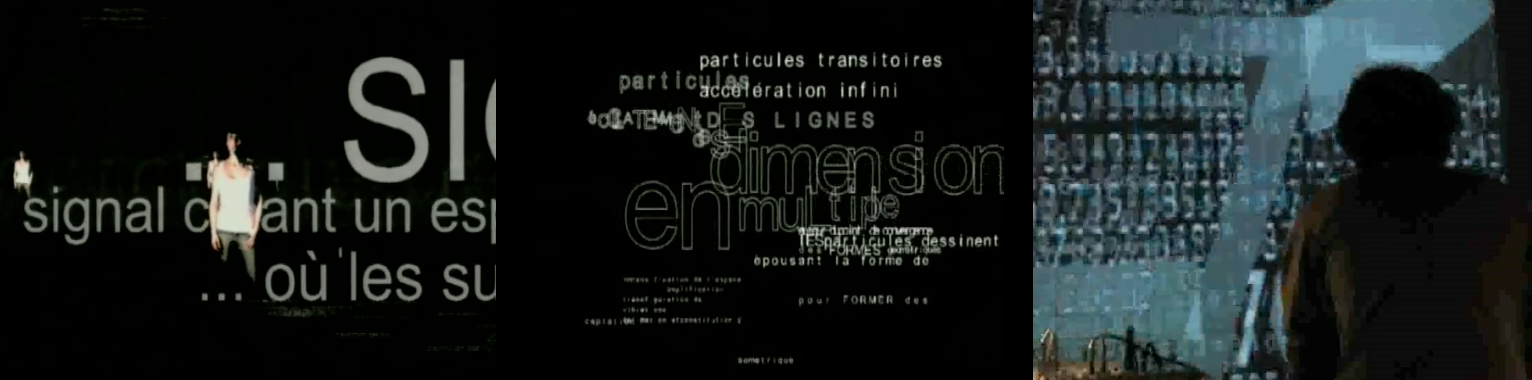
\includegraphics[width=1\textwidth]{pictures/cap1/hp1}
\caption{Detalhes da performance HP Process, apresentada na PdCon de 2009.}
\label{fig:hp}
\legend{Fonte: \url{http://databaz.org/xtrm-art/?p=439}}
\end{figure}

Apesar todo esse interesse em música e de começar a estabelecer uma produção voltada para ela, o campo disciplinar onde estava inserida como pesquisadora ainda era o do design, e a partir dele comecei a desenvolver algumas práticas em vídeo e música visual. Em parceria com Amer Moussa, no Coletivo 24h, fizemos em 2009 experimentos com colagens de vídeos como Pink Flamingos, Copacabana Mon Amour e A Mulher de Todos, sobrepostas a animações geométricas psicodélicas, que apresentamos na festa Perversa, no clube Glória (Perversa hum 01 - Coletivo 24h). Na época, fazíamos as animações em Flash, e utilizamos softwares de edição de vídeo para criar vídeos estáticos, inspirados em trabalhos como os de Marcel Duchamp e Norman McLaren. 

A com esse contato mais próximo com a comunidade do PD, comecei a desenvolver um \emph{patch} para processamento de áudio e vídeo em tempo real, que foi utilizado nas performances do projeto Cromocinética do Coletivo 24h. O patch interligava até três computadores: em um deles era feito o controle da ordem dos vídeos, a partir de uma biblioteca de loops de vídeo produzidos por Amer Moussa; no outro era controlado o som, produzido por Fernando Bizarri (Organograma) no Buzz; o Buzz enviava o sinal de áudio e informação MIDI para um terceiro, onde se controlava as formas geométricas que eram processadas em tempo real a partir do envelope sonoro do áudio, passando por um filtro que separava as frequências graves e as agudas, gerando sempre uma composição de formas diferentes – mas sempre muito concretas – em movimento frenético sincronizado com o áudio. \footnote{Um trecho do vídeo da performance ocorrida no MIS está disponível no youtube em:  \url{https://www.youtube.com/watch?v=_ZsqAX7roBM}.}

\begin{figure}

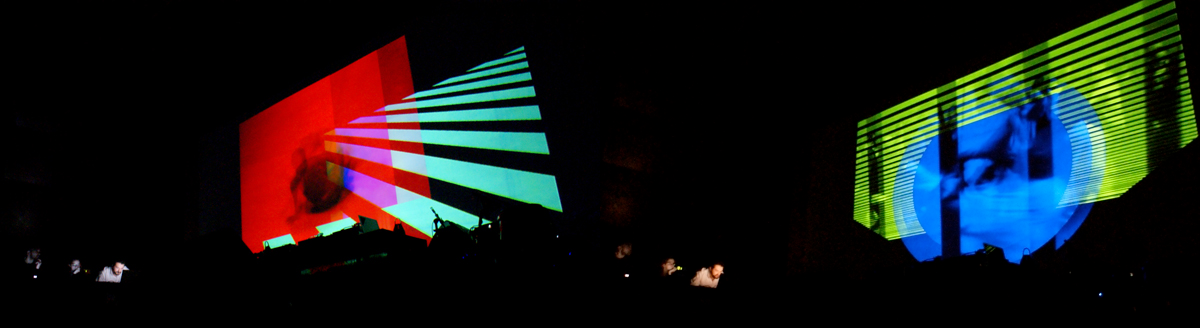
\includegraphics[width=1\textwidth]{pictures/cap1/cromocinetica}
\caption{Fotos da performance audiovisual Cromocinética.}
\label{fig:cromocinetica}
\legend{Fonte: \url{http://databaz.org/xtrm-art/?p=439}}
\end{figure}

O \emph{patch} foi construído de forma modular. Comecei desenvolvendo figuras mais simples, como os círculos e triângulos até chegar em estruturas mais complexas como grids e listras, conforme ia desenvolvendo o aprendizado em programação no software. Essas primeiras experiências com PD começaram a tornar a possibilidade pesquisa na música mais palpável, mas ainda estavam muito distantes do percurso acadêmico que estava percorrendo até então, que tinha como questão central a world wide web e suas tecnologias.

\subsection{Essa é pra tocar}
Em 2014, fui convidada por Daniel Scandurra e Gabriel Kerhart para pensar no desenvolvimento de uma obra de arte interativa para compor a exposição Gil 70, de curadoria de André Vallias, em comemoração dos 70 anos do cantor Gilberto Gil, que aconteceu em 2014. Daniel estava desenvolvendo um projeto chamado Moisacages\footnote{http://mosaicages.blogspot.com.br/}, onde compunha mosaicos com vários vídeos no Youtube, para serem tocados simultaneamente pelos visitantes de seu blog, e a idéia era produzir alguma obra interativa nesse sentido. Pensamos em construir uma espécie de instrumento audiovisual que funcionasse como uma máquina de montagem a partir de fragmentos sonoros.

\begin{figure}

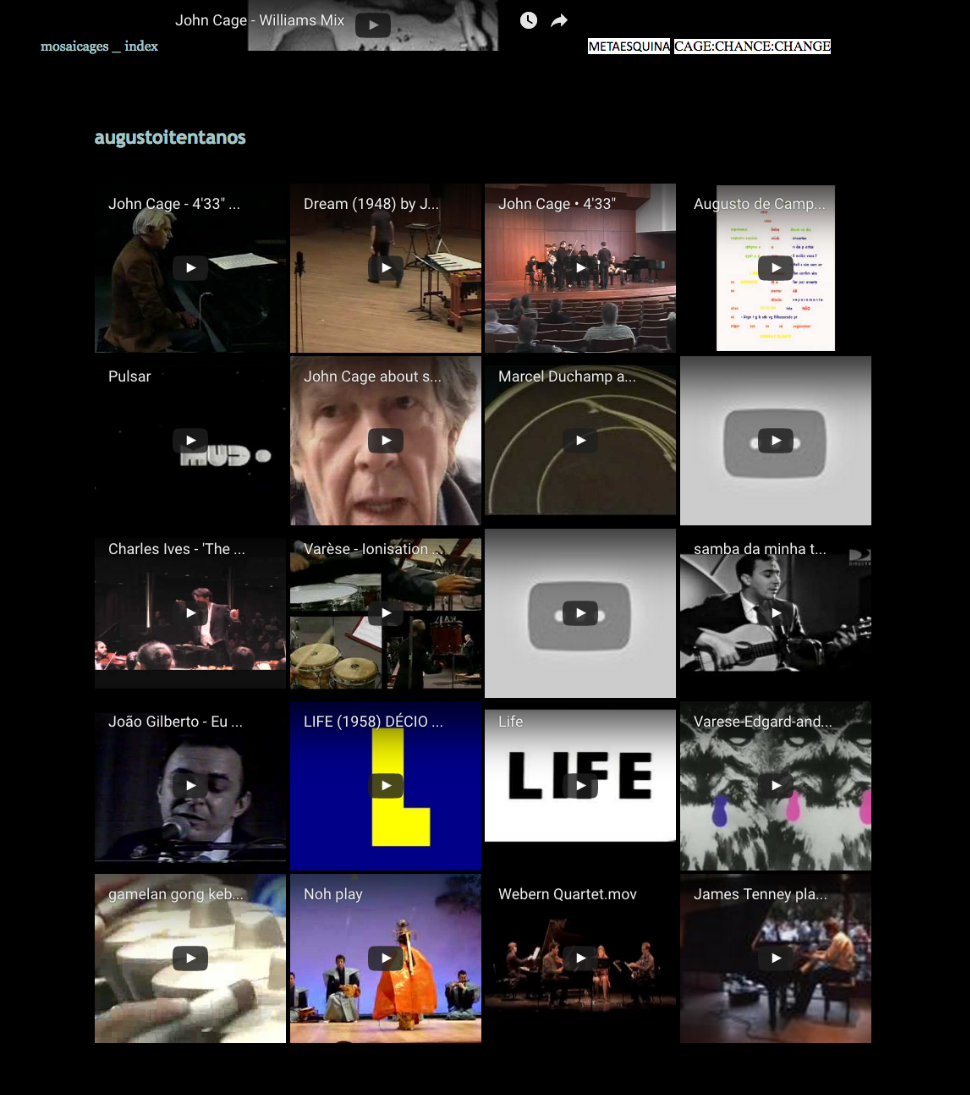
\includegraphics[width=0.8\textwidth]{pictures/cap1/mosaicages}
\caption{Mosaicage em Homenagem a Décio Pignatari, de Daniel Scandurra.}
\label{fig:hp}
\legend{Fonte: \url{http://mosaicages.blogspot.com.br/2011/02/augustoitentanos.html} Screenshot da autora em Janeiro de 2017.}
\end{figure}

Era importante para nós que a obra fosse interativa em um sentido imersivo, que convidasse o público a participar e desse possibilidade de se passar um tempo mergulhado, e não queríamos que fosse uma coisa que ficasse soando constantemente durante a exposição, uma obra viva que só funcionasse a partir de uma ação concreta. 

Naquele ano, haviam sido lançadas as especificações do HTML5 e o navegador Firefox tinha passado a dar suporte à tag <audio> em páginas da internet. Isso abriu perspectiva para desenvolver a obra diretamente usando um navegador de internet como suporte. Pensamos em criar uma página que funcionasse como um instrumento musical, onde o público poderia compor com fragmentos da obra do cantor, criando novas sonoridades a partir da sobreposição de samples. 

Como designer, atuando na produção de jornais e revistas acadêmicas durante a graduação, um processo que foi fundamental na prática compositiva dos grupos que participei foi o da fotomontagem, especialmente durante a produção da Revista Contravento HUM!\footnote{A revista Contravento começou a ser produzida pelo LabHab Gfau em 2004. A partir do número HUM! (existiu uma número zero) passamos a incuir na revista também um conteúdo ficcional, que se alternava com  textos teóricos produzidos ou traduzidos pelo corpo editorial ou convidados.}. Usávamos uma técnica de fotomontagem com recortes de xerox. Posteriormente, como docente na Universidade Nove Julho, ministrando a disciplina Projeto da Imagem, utilizava a mesma técnica em para exercícios onde os alunos deveriam desenvolver imagens que pudessem transmitir certos conceitos de linguagem visual. O que eu constatei foi que, se a base original de imagens apresentadas para as montagens fosse consistente, a qualidade estética dos trabalhos apresentados melhorava significativamente. Um princípio semelhante poderia ser utilizado para pensar em montagems sonoras, procurando trechos significativos que funcionassem de maneira autônoma, e fazendo uma seleção de um repertório prévio. Com essa ideia em mente, fizemos uma varredura na obra musical de Gilberto Gil, separando fragmentos de som que dividimos em 6 diferentes grupos: 

\begin{description}
\item[falas,]{ como trechos de discurso e falas significativas, sem som de fundo;
}
\item[gilbertália,]{ que reunía tudo que fosse relacionado à outras pessoas, como gil cantando outros compositores;
}
\item[banda,]{ com trechos de canções com fundo musical com banda;
}
\item[voz e violão;]{}
\item[onomatopeias,]{ com trechos de gritos, berros, ou outros sons curtos muito característicos do cantor;}
\item[bases,]{ com trechos de áudio mais longos; 
}

\end{description}


Pensamos em uma estrutura em seis faixas, em uma referência ao I CHING, que chamamos de ``Hexagrama Essa é pra tocar''.  Cada faixa correspondia a uma categoria de samples, de modo que na tela sempre haveria a possibilidade de combinar arquivos de grupos diferentes. Desenvolvi uma estrutura em JavaScript que separava cada faixa de samples em arquivos HTML diferentes, de forma que os arquivos pudessem ser preenchidos em paralelo e um sistema de códigos para estilos e tamanho de texto que possibilitou que toda equipe trabalhasse diretamente no código, mesmo sem ter conhecimentos desenvolvidos em HTML. 
Cada arquivo HTML correspondia a uma faixa do hexagrama, que por si continha muitos samples. Esses arquivos eram carregádos na página através de tecnologia Ajax\footnote{Ajax é um acrônimo para ``Asynchronous Javascript and XML'', e é uma tecnologia baseada no \emph{XMLHttpRequest} que basicamente permite a alteração do conteúdos das páginas sem a necessidade de recarregamento. Ajax é base para a maioria das páginas e sistemas web atualmente.}. 

As faixas podiam ser arrastadas continuamente para cima e para baixo, infinitamente, de modo a permitir variadas combinações entre as elas, mas oferecendo sempre um número limitado de possibilidades na tela. Para criar esse efeito de rolagem infinita era necessário multiplicar os elementos na tela, então para não sobrecarregar o sistema, os objetos de áudio ficavam todos em um arquivo separado, e apenas as faixas eram processadas em tempo real manipuladas. 
Desse modo, conseguimos chegar em cerca de 800 samples de áudio, que na tela eram representados por trechos das letras, imagens ou símbolos, e GIFs animados. quando tocados, alguns dos samples disparavam em conjunto vídeos, na maioria trechos de filmes da tropicália, produzidos pelo cineasta Gregório Grananian. Os vídeos podiam ocupar toda a tela ou parte dela, GIFs às vezes se sobrepunham aos vídeos, criando uma montagem audiovisual em tempo real, dentro de uma ideia de cinema expandido.  

\begin{figure}

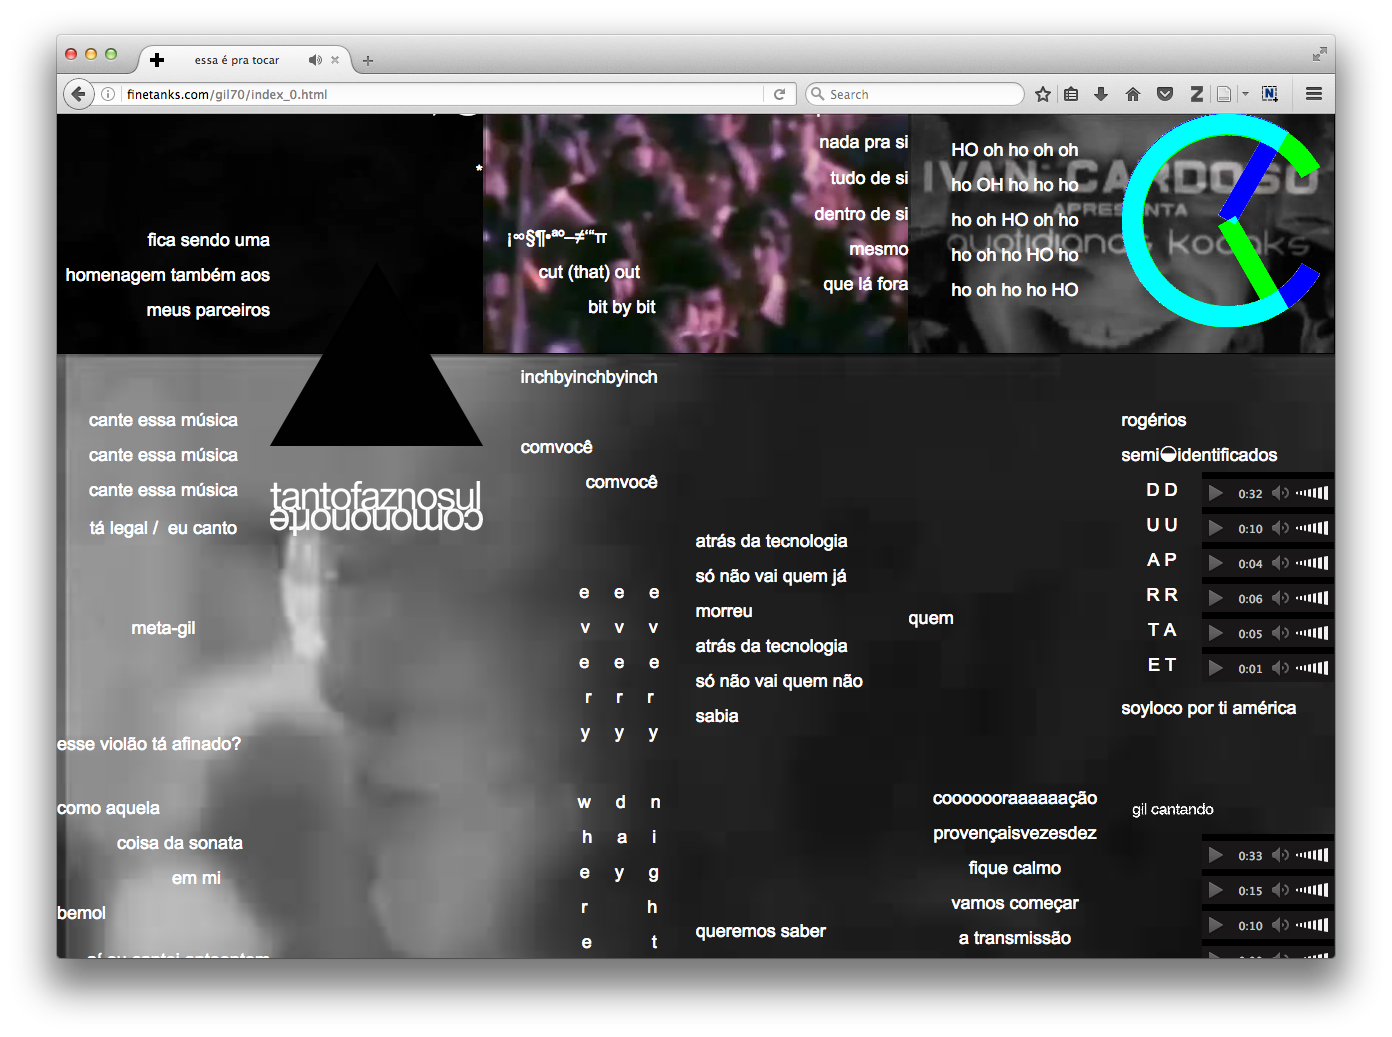
\includegraphics[width=1\textwidth]{pictures/cap1/gil701}
\caption{Interface do projeto ``Hexagrama essa é pra tocar''.}
\label{fig:gil701}
\legend{Fonte: Screenshot da autora}
\end{figure}

\begin{figure}

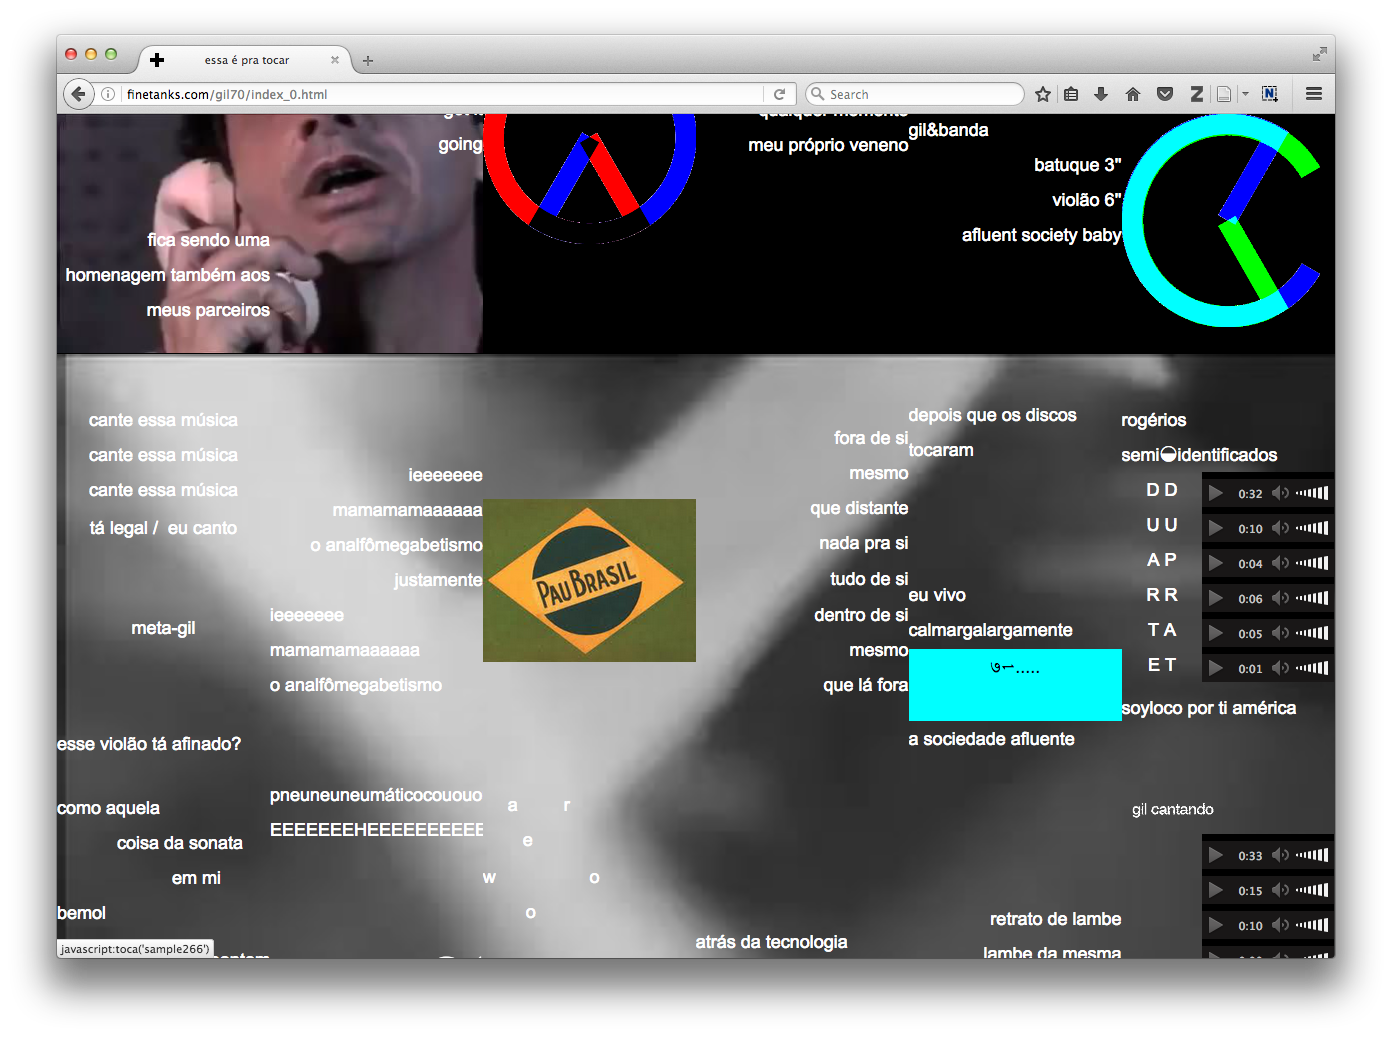
\includegraphics[width=1\textwidth]{pictures/cap1/gil702}
\caption{Interface do projeto ``Hexagrama essa é pra tocar''.}
\label{fig:gil702}
\legend{Fonte: Screenshot da autora}
\end{figure}

Durante a exposição, o site rodava em um totem com tela sensível ao toque no Firefox, a partir de arquivos em um computador local, sem necessidade de internet. Por ser baseado somente em HTML, CSS e JavaScript, o Hexagrama não depende de nenhuma tecnologia de processamento no servidor, então é bastante portável, podendo ser tocado diretamente de um pendrive, por exemplo. Isto facilitou sua montagem nos diversos locais onde foi exposto. Apesar de ter sido pensado como uma instalação interativa, existem algumas versões online que podem ser utilizadas abertamente até hoje. \footnote{Disponível em: \url{http://finetanks.com/gil70}.}
Além do totem com tela sensível ao toque, onde o público interagia com a obra, nas exposições no Rio de Janeiro, no Centro Cultural dos Correios e em São Paulo, no Itaú Cultural, usamos também um projetor, que reproduzia o site em tamanho grande e duas caixas de som omnidirecionais\footnote{As caixas foram projetadas e executadas pelo meu pai, Guido Stolfi, engenheiro eletricista e marceneiro entusiasta.}, que contaminavam todo ambiente expositivo com os sons disparados pela obra.

Esta primeira experiência em arte sonora baseada em tecnologias web, que também foi uma experiência de desenvolvimento de um projeto de interface de invenção, foi a ponta de lança para esse projeto de pesquisa. A partir da constatação práticas dos potenciais do uso de HTML, CSS e Javasçript, tendo o navegador como suporte, comecei a pensar na ideia de desenvolver instrumentos musicais, e isso pareceu o caminho que poderia unir o meu percurso de pesquisadora em design de interfaces web, que segui durante o mestrado, com o interesse nas práticas musicais, sobretudo experimentais, que estava desenvolvendo.


\newpage
% !TEX encoding = UTF-8 Unicode
% !TEX root = tese.tex
\chapter{Interfaces para produção sonora}
\label{ch:pesquisa}
Nesse capítulo, apresento o início deste processo de pesquisa, da compreensão da problemática da questão da interface na produção musical ao mapeamento das experiências disponíveis no momento. Durante o mestrado\footnote{\cite{Stolfi}}, pesquisamos interfaces web e suas tecnologias. Agora o surgimento do HTML5 e das tecnologias de web áudio, aliado ao desenvolvimento do trabalho em homenagem a Gilberto Gil, que demonstrou que havia muita possibilidade na utilização criativa dessas novas tecnologias, apontaram uma possibilidade concreta de dar prosseguimento à pesquisa acadêmica na área da música.

Antes do HTML5, tudo que envolvia processamento de áudio em tempo real em páginas de internet era embasado em softwares proprietários como o \emph{Flash}, ou em \emph{plugins} programados em alguma linguagem de baixo nível como Java, Python ou C++. O HTML5, junto com a WebAudio API, que estabelece parâmetros para processamento de áudio em JavaScript, permite que agora seja possível o controle de processos de áudio diretamente pelos navegadores, sem a necessidade de instalação de nenhum programa adicional. Um site como o Radio.garden, que mencionamos na introdução deste trabalho, por exemplo, possui uma interface que só é possível graças ao desenvolvimento dessas novas tecnologias de \emph{streaming} de áudio e geoprocessamento em 3D via JavaScript, que faz com que o grosso do processamento aconteça no computador do usuário, e não no servidor. Isto diminui os recursos necessários da parte do servidor para rodar o site, diminuindo também os custos dos sistemas que fazem uso dessas tecnologias.

Nossa hipótese era que utilizando essas tecnologias, poderíamos criar instrumentos musicais que explorassem possibilidades de inter-relação audiovisuais, acessíveis e que possam funcionar em qualquer computador que tenha instalado um navegador que suporte esses novos recursos, podendo funcionar inclusive localmente em máquinas sem acesso à internet e dispositivos móveis. Partimos da ideia de que seria possível utilizar criativamente essas tecnologias para propor novas interfaces para expressão musical.
    
A ideia inicial, era trabalhar em alguns projetos de instrumentos musicais, que pudessem ser usados por qualquer um para compor ou performar música eletrônica. Desde o início, ficou claro que essa pesquisa tinha um caráter bastante interdisciplinar, partindo do design, mas abarcando questões como interação humano computador (IHC), semiótica, computação musical, música experimental, filosóficas e políticas.

No artigo ``Logics of interdisciplinarity'', Barry, Born e Weszalnys apontam o campo interdisciplinar da Arte-ciência, como um campo emergente, onde ``a prática corre na frente da teoria'' \footnote{\cite{Barry2008}}, que pode ter como um dos objetivos ``desafiar e transformar formas existentes de pensar sobre a natureza da arte e da ciência, bem como as relações entre artistas e cientistas e seus objetos e públicos'', segundo eles, invenção e originalidade na arte-ciência se sustentam melhor nas práticas onde os artistas conseguem fazer uso de laboratórios, oficinas e computadores \footnote{(idem, p. 39)}. Isto é reforçado se observarmos os trabalhos de alguns pioneiros da arte digital, como Erthos Albino de Souza, Waldemar Cordeiro, Nam Jum Paik e Júlio Plaza. Plaza aponta que intermídia e multimídia são ``categorias interdisciplinares  que colocam em questão as formas de produção-criação individual''\footnote{\cite[p. 66]{JulioPlaza1969}} e que as formas eletrônicas tem um caráter abrangente que dialoga ``inter sensorialmente '' com vários códigos da informação, ``uma hibridização de meios, códigos e linguagens que justapõem e se combinam'' \footnote{(idem, p. 13)}

A interface é considerada pelo campo de estudos de IHC, como “uma fronteira através da qual dois sistemas se comunicam (o humano e o programa)” \footnote{\cite{Magnusson2005}}, ou a parte visível de um sistema complexo, método ou classe, segundo a definição da engenharia de software: uma base de controle simples e inteligível que permite às pessoas um controle de alto nível sobre estruturas subjacentes. Ela pode ser considerada um sistema de comunicação, pois “conecta dois agentes e objetos” criando “um espaço sígnico comum a esses agentes” \footnote{\cite[p. 105]{IAZZETTA1997}}. Ao mesmo tempo que permite que uma pessoa comunique certas coisas a um software, por exemplo, ela também é o que comunica coisas à pessoa sobre o software. Magnusson (\citeyear{Magnusson2005}) defende que a própria interface pode ser vista como uma ideologia musical: 
%[212]

\begin{citacao}
A interface é um instrumento. É uma manifestação gráfica de ideias musicais e processos de trabalho. A interface é ao mesmo tempo a plataforma estética definindo as estruturas musicais e a base prática de controle para o sistema sonoro subjacente. De um certo modo pode ser vista como uma ideologia musical. Ela define possibilidades, mas também define as limitações do que pode ser composto ou tocado. Aqui nós estamos pensando principalmente nas interfaces gráficas de softwares de áudio, mas esse argumento pode ser estendido às linguagens de programação de áudio também: os objetos e classes pré-programados à disposição em uma dada linguagem definem o que pode ser expressado. \footnote{\cite[p. 212]{Magnusson2005}, tradução nossa.}
\end{citacao}


\subsubsection{\emph{Bootstrapping}}

Uma referência fundamental no campo de pesquisa do design de interfaces é Douglas Engelbarth, que com o trabalho no Augmentation Research Center (ARC), deu origem a uma série de recursos fundamentais para IHC. Em 1962, as companhias já tinham desenvolvido o computador, que era utilizado principalmente como ferramenta militar ou de suporte à grande indústria. Eram grandes máquinas compartilhadas com interface mediada somente por texto. A pesquisa no ARC procurava aplicar o potencial do computador como ferramenta para ampliação do intelecto humano\footnote{\cite{Engelbart1962}}, para além das finalidades bélicas e industriais. Em 1968, Engelbarth apresentou os resultados das pesquisas do ARC em uma apresentação em São Fanscisco que ficou conhecida como ``The mother of all demos'', onde demonstrou ao vivo recuros como o mouse, o primeiro editor de texto, e o conceito de espaço visual no computador, recursos que foram fundamentais na história da computação. 


O trabalho do laboratório, que desencadeou em transformações radicais nas tecnologias posteriores, era baseado em uma metodologia que chamavam de \emph{bootstrapping}, que se tratava basicamente em buscar construir ferramentas para o próprio trabalho, no caso, o de programação dos computadores compartilhados da época.  


\begin{figure}
    \caption{\label{motherofalldemos}Trechos da apresentação de que ficou conhecida como ``The Mother of all demos'' em 1968.}
    
        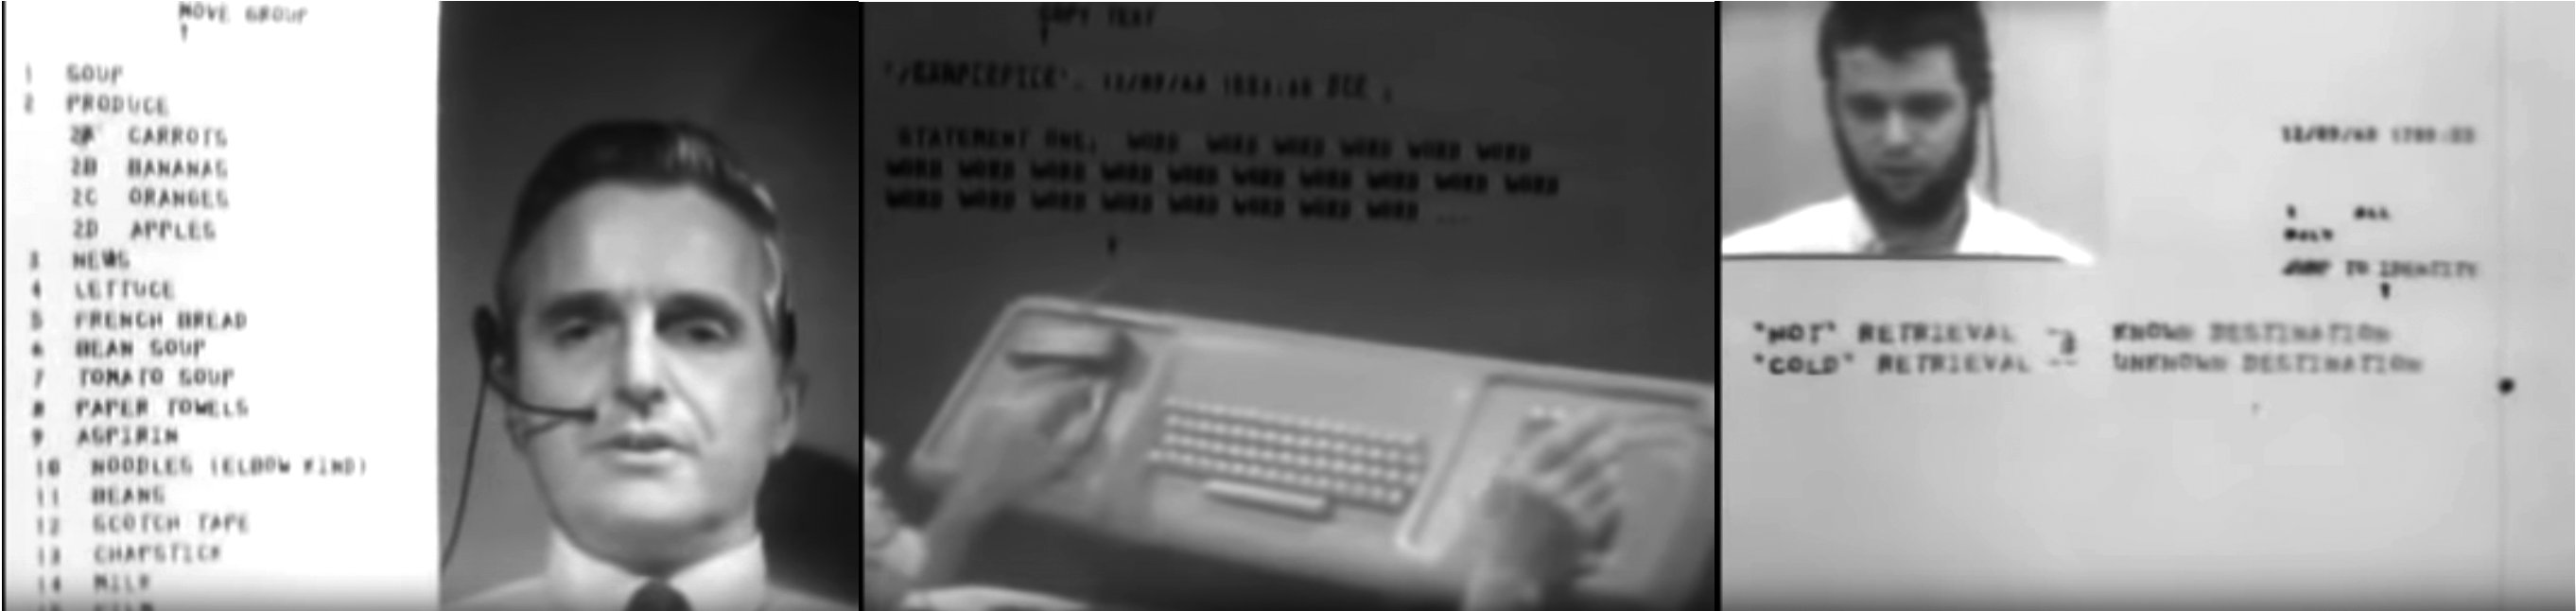
\includegraphics[width=1\linewidth]{pictures/cap2/mother_of_all}
    
    \legend{Fonte: Screenshot da autora do vídeo disponível em \url{https://youtu.be/yJDv-zdhzMY} no dia 20 de dez de 2017.}
\end{figure}



Pensar na ideia de \emph{bootstraping} como metodologia de trabalho fez, de uma certa maneira, mudar o foco inicial desta pesquisa, que era inicialmente de construir coisas genéricas para um usuário genérico --- como é tradicionalmente a metodologia do design --- para procurar construir instrumentos que fossem, acima de tudo, ferramentas para a nossa própria pesquisa prática em música experimental, individual e coletiva, junto a redes como NuSom, Sonora, Tecnoxamanismo, BlóKõKê, Orquestra Errante entre outras.

\subsubsection{\emph{Bootstrapping} na música}

Na história da música existe uma série de casos onde a ideia de desenvolver seus próprias tecnologias para produção sonora moveu parte da pesquisa dos músicos. Uma pessoa que teve essa abordagem foi Daphne Oram, precursora da música eletrônica que desenvolveu um sintetizador de música baseado em desenhos. O Oramics funcionava através de desenhos que definiam envelope, e perfil melódico do som. Oram observou que a música eletrônica dital na época era regida principalmente por ``processos impositivos'', principalmente baseados em tom, volume e duração, ou baseados em sons puros, como de osciladores, ou em desenhos de onda definidos digitalmente, que segundo ela ``tinham pouca finesse'' \footnote{\cite[p. 101]{Oram1972}}: 

\begin{citacao}
One of the points to notice in digital computer music is the
quality of each note ... its timbre, its subtlety, its individual shape and phrasing. When you come to program your digital computer will you, mostly, be concerned with the regulation of pitch and rhythm and interval relationship? Will you be able to give time, also, to considering the beauty of each individual note... the subtle individuality of each note ... as well as its place in the main scheme? Will each note, each phrase or melisma, be able to affirm the richness and the character of its own individuality, while it is taking its balanced position in the overall structure? 

We wish to design this machine-with-humanising-factors so that the composer can instruct it by means of a direct and simple language. He will want to transduce his thoughts as quickly as possible, via a channel which is logical. \footnote{\cite[p. 97]{Oram1972}}
\end{citacao}

Seu desejo era de criar uma máquina em que ela pudesse desenhar os sons, e para tanto, ela passou muitos anos desenvolvendo a ideia dessa máquina até que conseguiu recursos para construí-la. O Oramics, foi no entanto, uma máquina única, desenhada pela e para a própria autora --- na busca de expressar seus desejos estéticos composicionais --- e nunca chegou a ser um produto comercializado nem produzido em série.   

\begin{figure}
    \caption{\label{oram}Daphne Oram e o Oramics.}
    
        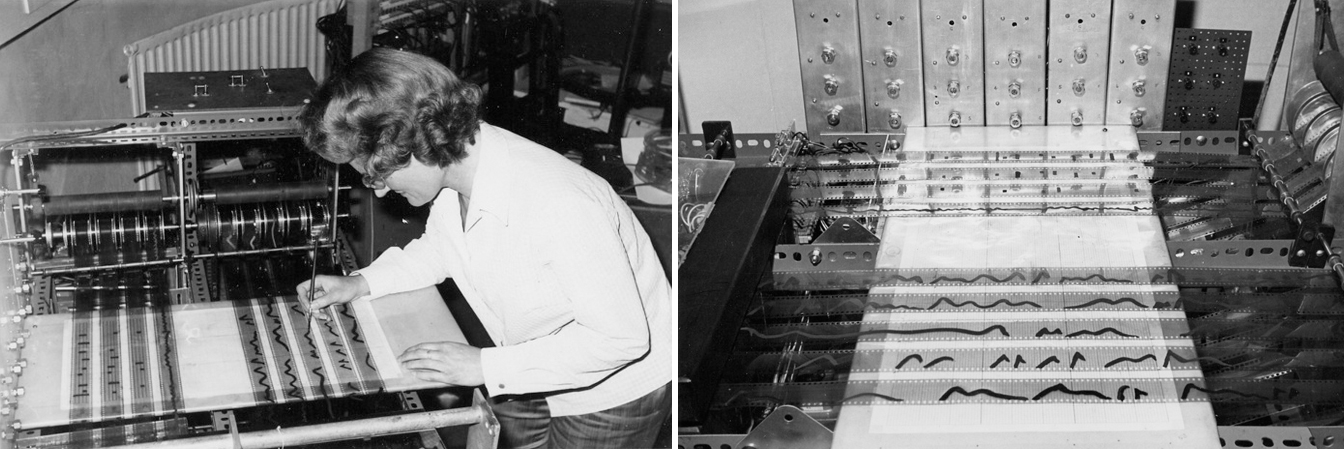
\includegraphics[width=1\linewidth]{pictures/cap2/oramics}
    
    \legend{Fonte: \cite{DavidCranmer2009}.}
\end{figure}


Outros que também desenvolveram seus próprios intrumentos para trabalhar com música foram os irmãos John and James Whitney, considerados precursores da música visual, que nos anos 60, criaram um sistema mecanizado baseado em um conjunto de pêndulos, capaz de escrever ondas senoidais na faixa de som de uma película cinematográfica; uma impressora sonora, como John explica abaixo:

\begin{citacao}
Nosso instrumento de som subsônico consistia em uma série de pêndulos ligados mecanicamente a uma cunha ótica. (...) Nenhum som audível era gerado pelo instrumento. Ao invés disso, uma trilha sonora ótica de dimensões padrão era sinteticamente exposta no filme, que depois de processado podia ser tocado em um projetor de filmes padrão."\footnote{\cite[p. 152]{Whitney1980}, tradução nossa} 
\end{citacao}

\begin{figure}
    \caption{\label{witney}Três imagem extraídas do filme ``Five Abstract Film Exercises'' de John e James Whitney.}
    
        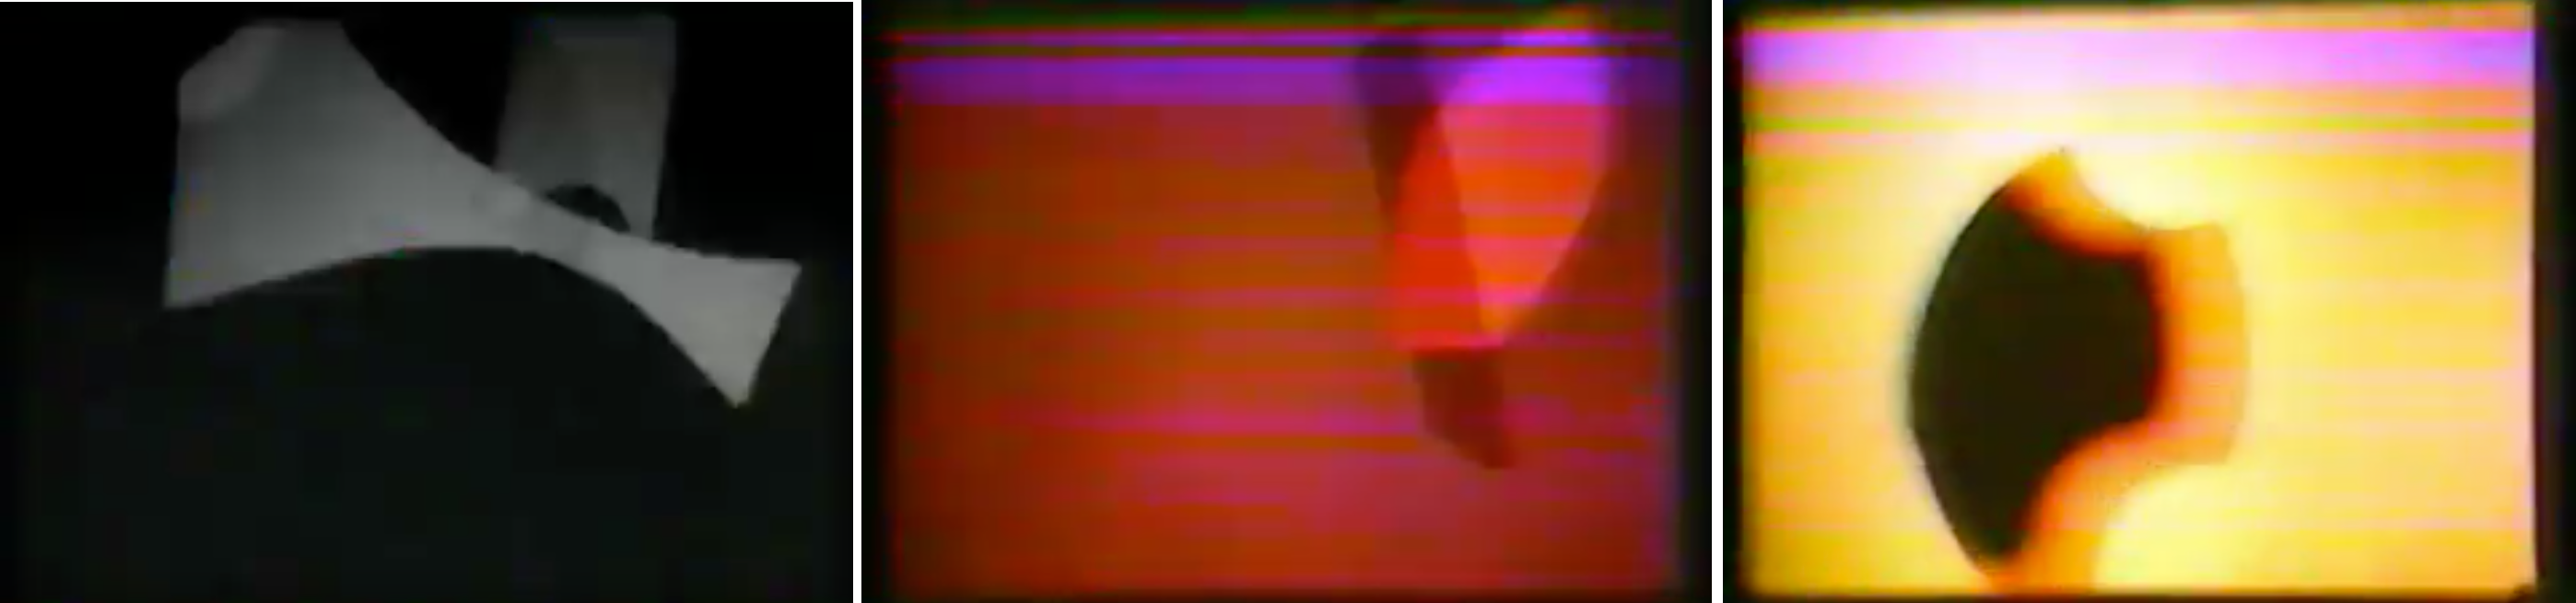
\includegraphics[width=1\linewidth]{pictures/cap2/witney}
    
    \legend{Fonte: Screenshots da autora.}
\end{figure}


Com esse instrumento, eles fizeram os filmes``Five Abstract Film Exercises''. O resultado sonoro, que trazia ondas puras senoidais e até glissandos foi chocante para época, e garantiu à dupla o prêmio pelo som na competição de filmes experimentais de Bruxelas de 1949\footnote{Disponível em: \url{https://www.youtube.com/watch?v=kuZbgM8yxtY}}.


Enquanto seu irmão James, foi com o tempo passando a se voltar mais à pintura e a questões místicas e de espiritualidade, John procurou a se dedicar mais ao desenvolvimento tecnológico e a sistematizar um pensamento sobre música e linguagem visual. Ao longo dos anos ele foi desenvolvendo um computador mecânico analógico, especialmente para animação com tipografia\footnote{\cite{Youngblood1970}}, prestando serviços para a indústria de filmes. Colaborou com Saul Bass na famosa abertura para o filme Vertigo, de Hitchcock, por exemplo. Sua máquina era formada por câmeras e mecanismos rotativos capazes de produzir imagens em movimento no filme a partir de moldes de cartolina e cálculos matemáticos complexos.  Whitney usou como base para seu primeiro computador analálogico um dispositivo antimísseis M-5, ressignificando um equipamento militar, ou nas palavras de Youngblood, ``uma arma da morte'' em uma máquina capaz de produzir beleza\footnote{\cite{Youngblood1970}}.

Suas pesquisas com o computador analógico levaram em 1966 a IBM se tornar a primeira empresa a abrigar um artista em residência, para explorar as potencialidades estéticas da computação. O filme ``Permutations'', seu primeiro desenvolvido em um computador digital, era considerado por John como o desenvolvimento de um novo modo de comunicação. Com a IBM, Whitney começou a trabalhar com o computador digital, que não exigia mais a necessidade dos estênceis analógicos. \footnote{\cite{Youngblood1970}}. 
Em seu livro ``Digital Harmony --- on the complementarity of musical and visual art'', publicado em 80, Whitney defende uma idéia de harmonia que ultrapassa a esfera da música, ``um contexto mais amplo no qual as leis Pitagóricas da harmonia operam''. Em seus filmes ``Permutations'' (1968) , ``Matrix I'' e ``III'' (1970 e 1972), e ``Arabesque'' (1973), Whitney programa formas em movimento segundo parâmetros matemáticos inspirados na harmonia de músicas de outros artistas, como Terry Rilley (Matrix III) por exemplo, procurando interpretar princípios harmônicos e rítmicos como formas e processos geométricos no tempo. Passou a perseguir a ideia da construção de um instrumento que fosse capaz de gerar som e imagem simultaneamente e em consonância. Esse instrumento partiria de parâmetros harmônicos do som, que eram mapeados em forma de coordenadas polares ou cartesianas. \footnote{\cite{Whitney1980}}

\begin{figure}
    \caption{\label{matrix}À esquerda, quadros do filme Matrix. À direita, a correlação gráfica da harmonia entre as notas musicais.
.}
    
        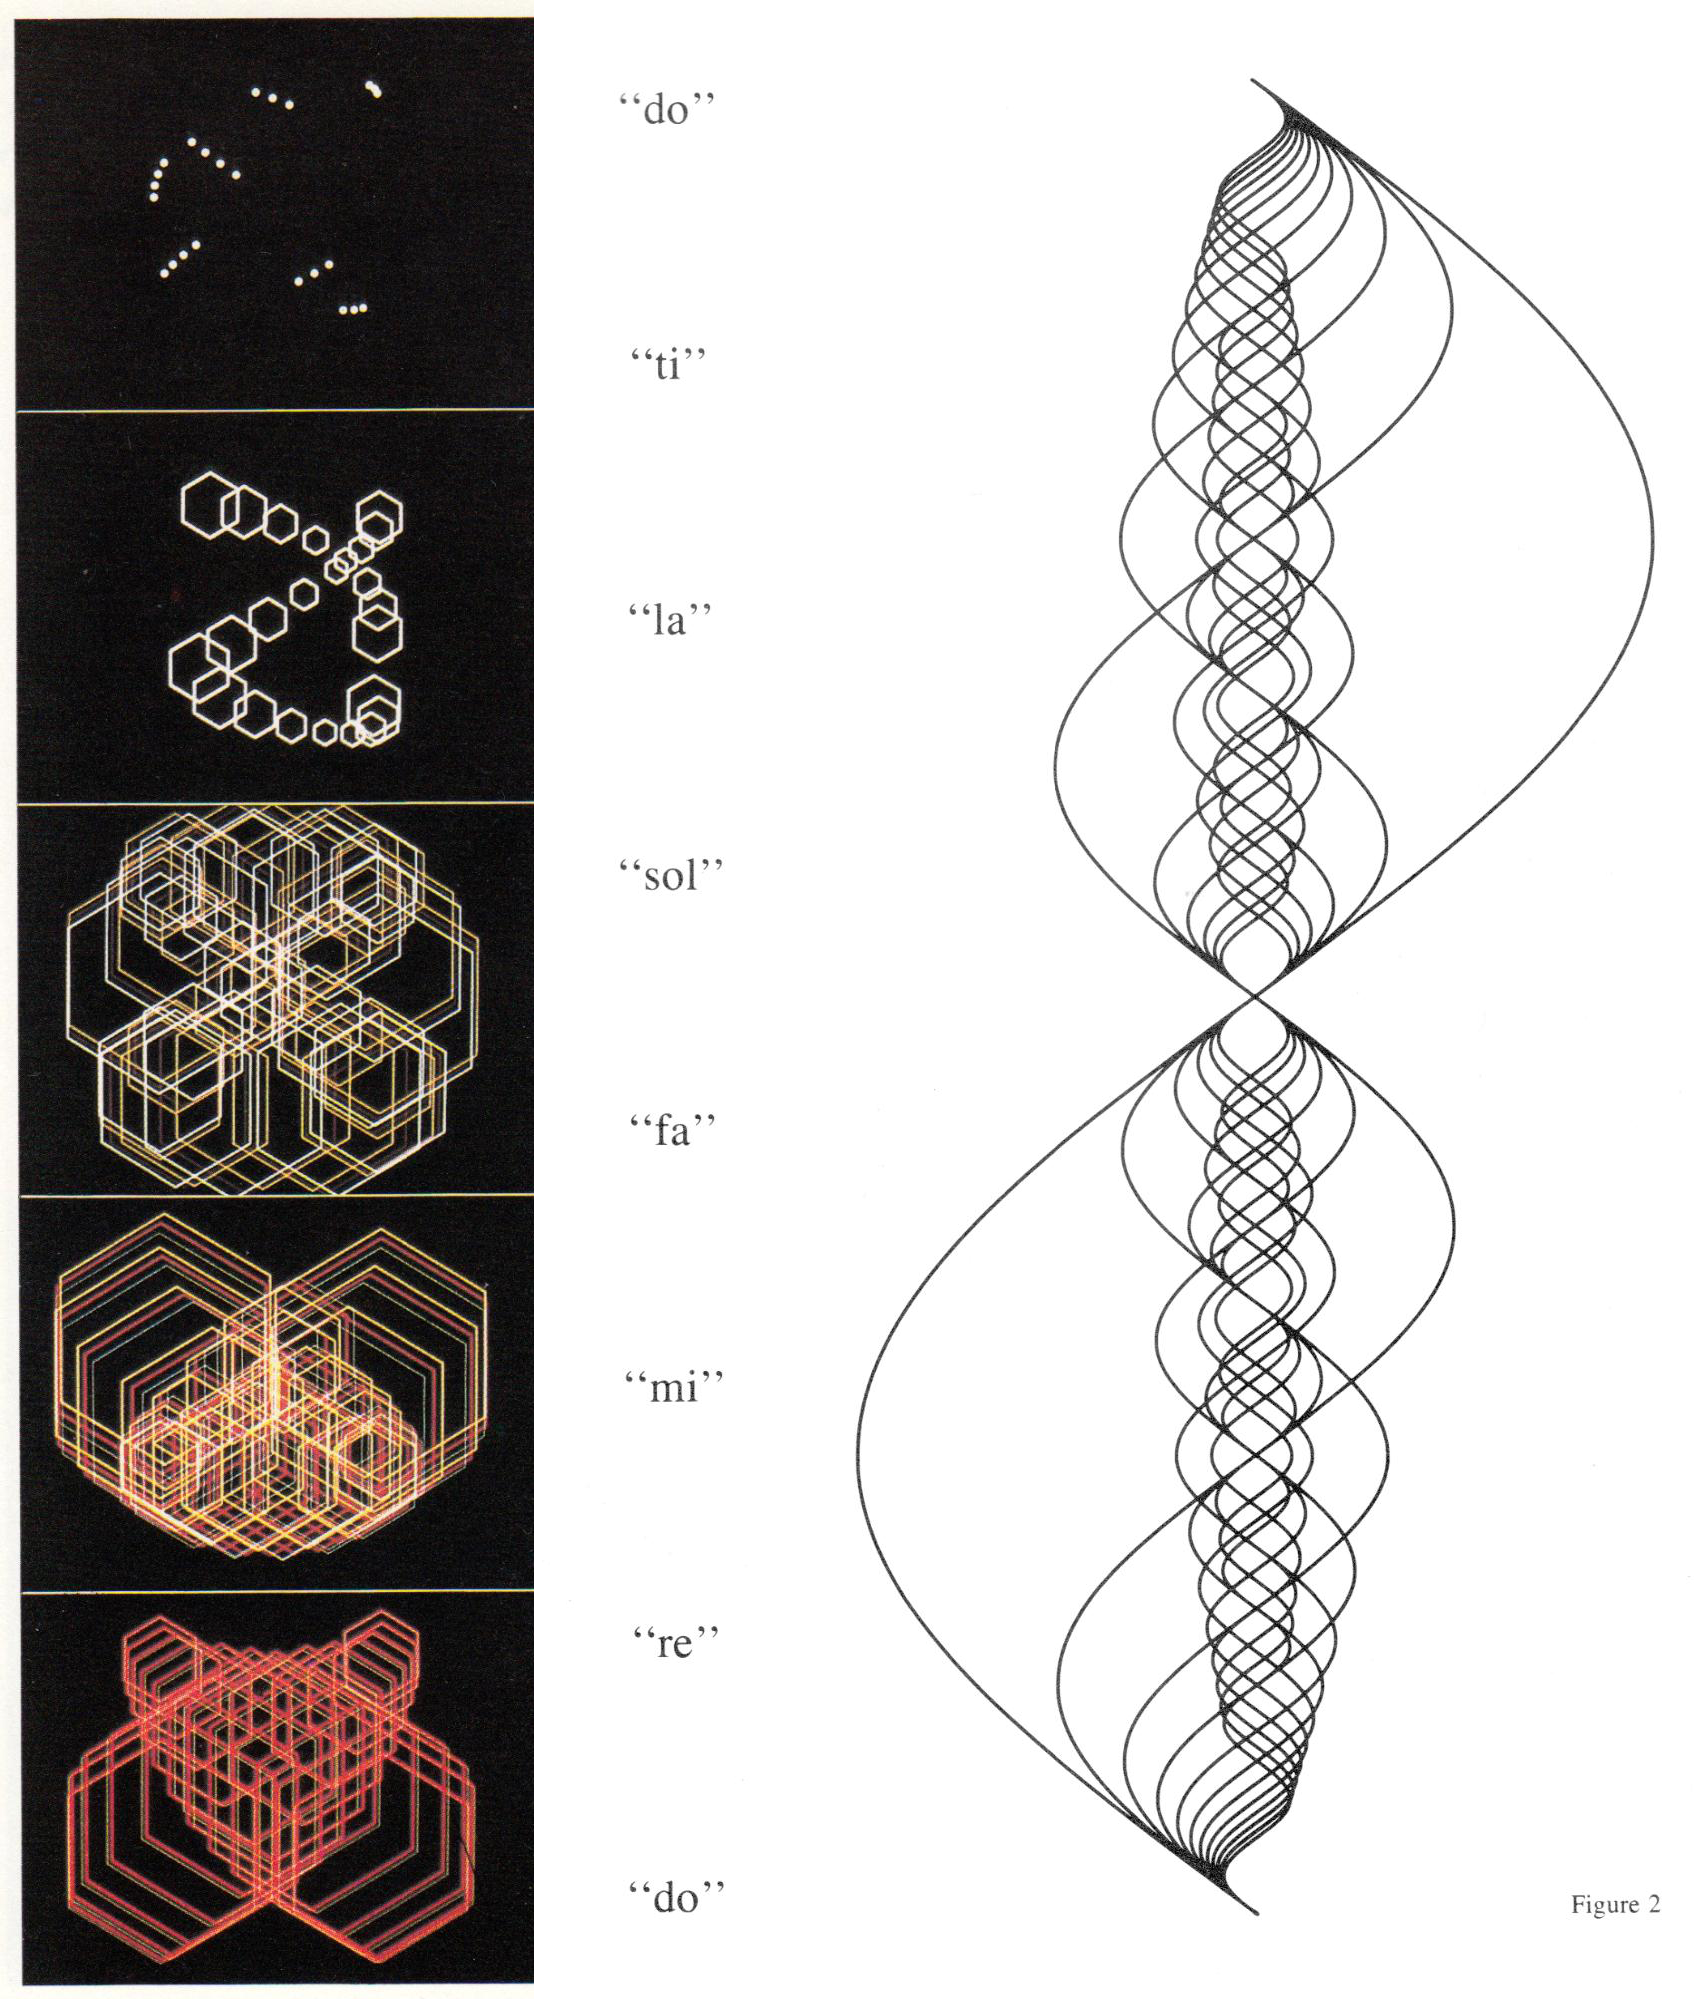
\includegraphics[width=0.8\linewidth]{pictures/cap2/witney2}
    
    \legend{Fonte: \cite{Whitney1980}}
\end{figure}


Outro que pesquisou com novas interfaces para produção de novas formas de música foi Iannis Xenakis, arquiteto e pioneiro na música experimental do século passado. Xenakis também foi vanguarda no pensamento da relação entre matemática, som e sua relação com arquitetura e o espaço, criando música a partir de relações matemáticas do desenho de frequências dentro do espectro sonoro. Desenvolveu novas formas de notação musical para abarcar suas experiências que fugiam do padrão tonal de composição tradicional, como aponta Crististiano Figueiró \citeyear{figueiro2013influencia}:

\begin{citacao}
Xenakis (1996), aponta o uso de um espaço multidimensional como auxiliar na representação das características de um som como um gráfico que auxilie a composição, ordenando cada característica de um som como altura, amplitude, tempo, densidade, desordem, parâmetros de timbre, etc..; onde cada característica é uma linha dimensional, e os sons, pontos paralelos em várias dimensões \cite{figueiro2013influencia}
\end{citacao}

Xenakis defendia que tudo é sujeito às leis da lógica e suas operações, como adição, subtração e intersecção, por exemplo, e sendo assim, "a música poderia ser definida como organização de operações elementares entre funções de entidades sonoras”.\footnote{\cite[p. 21]{Xenakis1971}}. Ele se amparou no desenvolvimento da tecnologia de processamento digital de áudio nos anos 70 para desenvolver, junto à sua equipe no ``Center for Studies in Mathematical and automated Music em Paris'' o UPIC, uma ferramenta capaz de converter desenhos em som, em uma correspondência direta entre posição horizontal das linhas na partitura e as frequências audíveis pelo ouvido humano.


\begin{figure}
    \caption{\label{xenakis}Trecho de \textit{Mycenae Alpha} de Iannis Xenakis.
.}
    
        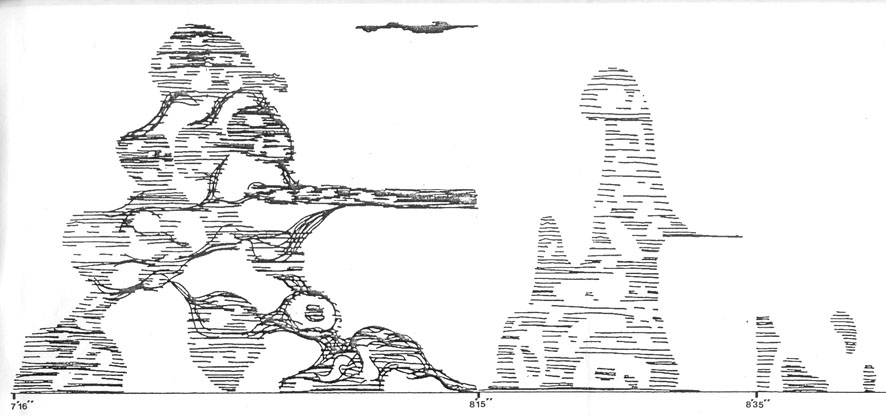
\includegraphics[width=1\linewidth]{pictures/cap2/metastasis}
    
    \legend{Fonte: \cite{Whitney1980}}
\end{figure}

%Uma outra referência importante para a pesquisa, está fora do campo do desenvolvimento de interfaces, a partitura visual de ``Artikulation'', de Gyorgy Ligeti, criada por Rainer Wehinger. Nela, as formas desenhadas correspodem a entidades sonoras da peça composta em fita. O trabalho não é uma representação literal do espectro gráfico da peça, mas uma leitura aproximada e sintetizada, num diálogo com princípios estéticos baseados também na teoria da forma (Gestalt).

%\begin{figure}
 %   \caption{\label{ligeti}Trecho da partitura visual criada por Rainer Wehinger para a peça Artikulation, de Giorgy Ligeti..}
    
 %       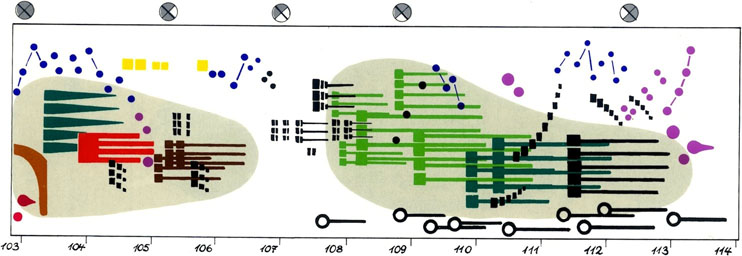
\includegraphics[width=1\linewidth]{pictures/cap2/ligeti}
    
  %  \legend{Fonte: \cite{Whitney1980}}
%\end{figure}


%\subsubsection{Brasil}
%Na cultura brasiliera, Anton Walter Smetak (Zurique, 1913 - Salvador, 1984), assim como o seu discípulo Marco Antônio Guimarães, são uma referência importante na pesquisa de intrumentos de invenção \footnote{\cite{Lima2018, Multimeios2001, Obici2014}}. Entre os princípios da sua prática estavam da pesquisa sonora de novos materiais, das necessidades do compositor ou do grupo, da modificação ou releitura de instrumentos tradicionais e da reciclagem de materiais diversos. Smetak construiu uma série de instrumentos que dividiu em algumas categorias: Instrumentos de sopro, percutidos, de percussão, a arco, plásticas sonoras, plásticas e instrumentos coletivos e diversos, que incluía um instrumento eletrônicos (o bicho) \footnote{\cite{Multimeios2001}}. 

%Seus instrumentos tinham uma forte característica escultórica, chegando a ``objetos plásticos de interatividade sonora'', como aponta Scarassati: ``de um lado o instrumento musical como um ponto de partida e, do outro, a escultura como um ponto de chegada, tendo a performance como a estrada que liga estes pólos''. Seus intrumentos, também não exigiam virtuosismo musical, como aponta o autor, facilitando seu uso no contexto de improvisação musical em grupo em que o compositor atuava. Também extraploavam os limites da música ocidental, abrindo perspectivas para o microtonalismo, onde segundo ele, ``não há o critério da afinação''. Smetak construiu cerca de 150 instrumentos musicais novos, ``utilizando materiais diversos, como cabaça, bambu, madeira, tubos de PVC, mangueiras plásticas etc.'' \footnote{\cite{Andres2011}}, movido por uma ``ideia de que uma nova humanidade requer uma nova música''. Em depoimento no vídeo documentário Smetak: Som e Espírito \citeyear{JessicaSmetakPaoli2010}, Smetak fala um pouco sobre sua inspiração:


%\begin{citacao}
%Cada objeto sonoro era um veículo para alcançar um novo plano de consciência. (...) Senti a responsabilidade que alguma coisa de mim devia se expandir, surgiram assim os primeiros intrumentos, qual batizei como nome de Choris, isso é, não chora nem ri. A improvisação um dia necessário para substituir a composição escrita. A idéia de um universo se aperfeiçoando, se ajustando com a interferência das artes e ciências em todos os setores. Efetuaram-se vários instrumentos de sons percutidos, os últimos com molas de aço amplificados eletrônicamente estourando-se na esfera da Caossonância que nos levou a múltiplas observações, mas levando sempre em consideração os citados dos sábios: ``que não há nada de novo embaixo do Sol''
%Tenho procurado diferenciar claramente o fazer som, um meio de despertar novas faculdades da percepção mental e o fazer música, apenas um acalento para velhas faculdades da consciência. \footnote{Walther Smetak, in \cite{JessicaSmetakPaoli2010}}
%\end{citacao}

%Quanto à autores contemporâneos, a tese de doutorado do pesquisador José Guilherme Allen de Lima \footnote{\cite{Lima2018}} ``Práticas de luteria na música experimental brasileira'', aprensenta uma panorama da luthieria experimental brasileira contemporânea, com uma pesquisa extensa de autores, espaços e tecnologias, principalmetne relativas a intrumentos físicos, muitos dos quais foram também desenvolvidos pelos próprios músicos que os tocam, como André Damião Bandeira, Cadós Snaches, Natacha Maurer e Marcelo Muniz, Arthur Jolly, Wilson Sukorsky, Pan\&Tone, LoopB entre outros.

%No campo da luthieria digital no Brasil, destacamos o trabalho de Jarbas Jacome, especialmente o ViMus, uma interface que faz a conversão em tempo real de áudio em imagens, e o trabalho de Jerônimo Barboza, que atualmente pesquisa na Universidade McGuill com Marcelo Wanderley, o Illusio, que parte de uma interface desenhável para criar um sistema de samplers capaz de gerar uma ``banda de um homem só''.  




%Thus, as discussed in (Fels, Gadd, \& Mulder, 2002), the task of keeping the adopter of the instrument engaged, involves designing for increasing complexity and expressivity as the player becomes expert.

%não se faz muita coisa sem software em música hoje em dia puckette

\subsubsection{Interfaces digitais}

Desde que os primeiros computadores estiveram disponíveis para pesquisa científica, músicos, compositores e pesquisadores têm desenvolvido interfaces para seu emprego em atividades musicais. Nos primeiros computadores a interface era física e a programação era operada por meio de cabos e potenciômetros diretamente no nível do hardware\footnote{\cite[p. 110]{Henrique1996}}. O ENIAC (1943 - 1946) (figura 1), um dos primeiros computadores construídos durante a Segunda Guerra Mundial com fins militares \footnote{\cite[p. 24]{Stolfi}}, era operado por pessoas com grau avançado de domínio da matemática, muitas das quais mulheres que já trabalhavam na guerra como computadoras fazendo manualmente cálculos de balística \footnote{\cite{HayleyWilliams2015}}, sua interface tem uma certa semelhança com a dos grandes sintetizadores modulares construídos anos depois, como o feito por Joseph Paradiso a partir de 1974, e que foi remontado em 2012 em uma exposição no MIT\ref{analogicos} de janeiro a abril de 2012. 

\begin{figure}
    \caption{\label{analogicos}À esquerda, interface do ENIAC.  À direita o sintetizador modular montado por Joseph Paradiso. }
    
    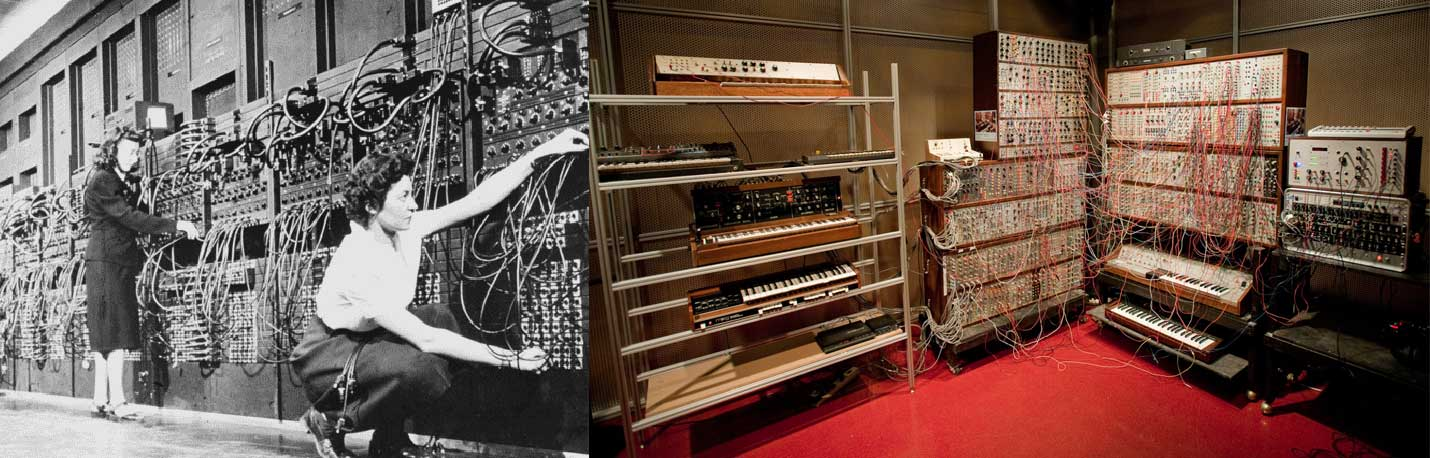
\includegraphics[width=1\linewidth]{pictures/analogicos}
    
    \legend{Fonte: \cite{HayleyWilliams2015} e http://web.media.mit.edu/~joep/pics/ FullSynthMIT-Museum.jpg}
\end{figure}

As primeiras experiências musicais em computadores digitais que se tem noticia foram realizadas na década de 50 por Max Mathews no ``Bell Telecom Lab''. Para gerar os primeiros sons computadorizados, Max teve que desenvolver uma linguagem de programação própria, que chamou de \emph{Music I} \footnote{\cite[p. 253]{Holmes1985}}. Depois de uma década desenvolvendo essa linguagem de programação musical, em 1968 passou a trabalhar no desenvolvimento do GROOVE (ou \emph{General Real-time Output Operations on Voltage-controlled Equipment}), um equipamento que funcionava na plataforma \emph{Graphic 1}, ``um sistema computadorizado interativo que podia traduzir imagens desenhadas com uma caneta luminosa em uma tela''\footnote{\cite[p. 253]{Holmes1985}}. Essa plataforma era similar à plataforma utilizada por Ivan Sutherland no \emph{Sketchpad}, pioneiro também dos programas de edição gráfica. O GROOVE teve a primeira interface gráfica interativa para computação musical. 

\begin{figure}
    \caption{\label{max}Max Mathews e L. Rosler com a estação de trabalho Graphic 1. }
    
        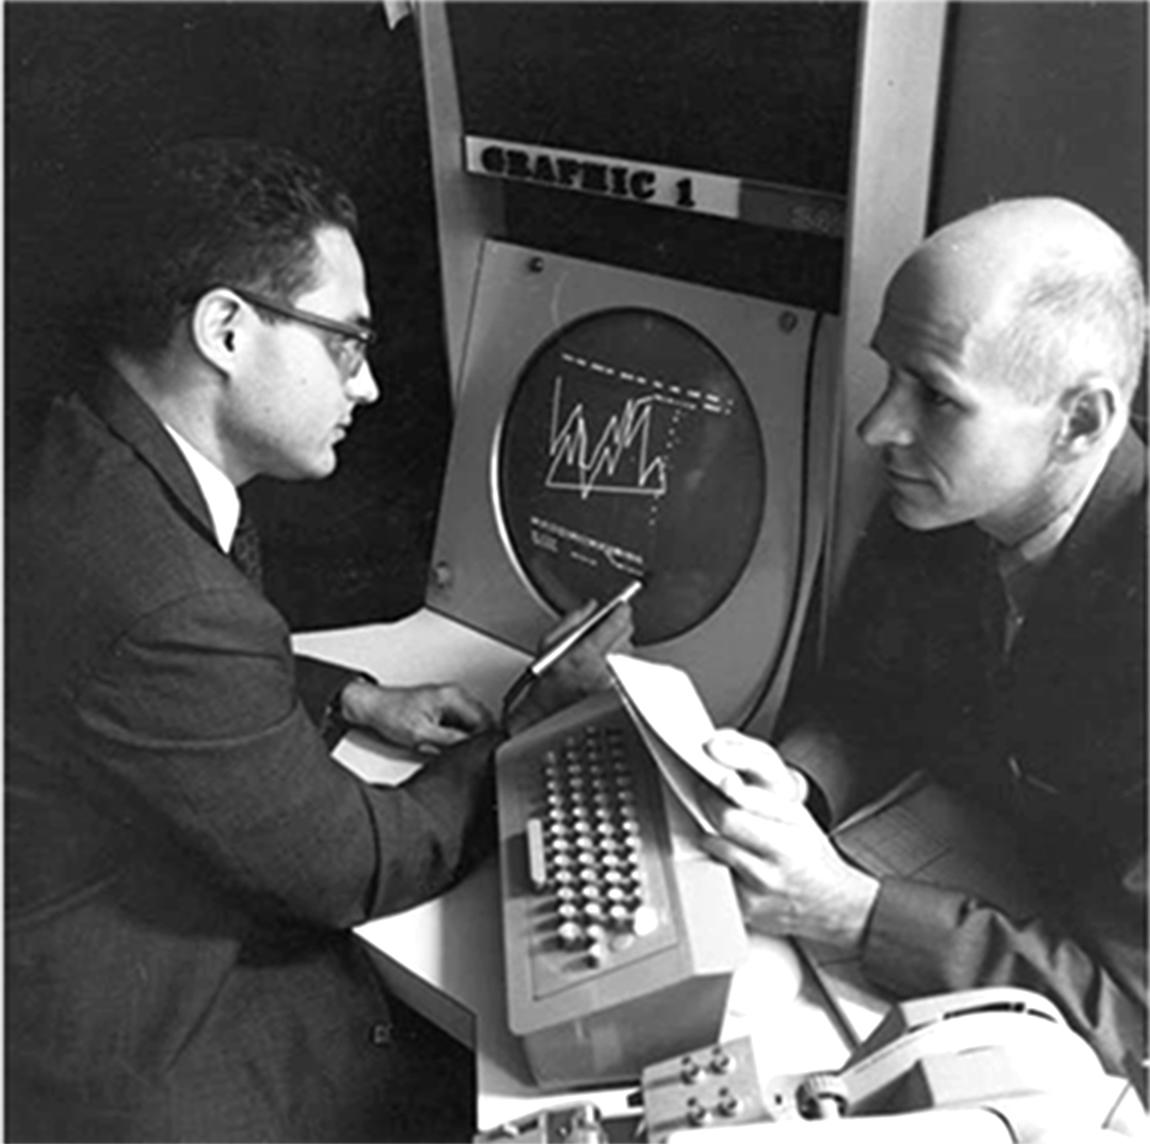
\includegraphics[width=0.5\linewidth]{pictures/MaxHolmes-251}
    
    \legend{Fonte: Holmes, 1985 p. 251}
\end{figure}

Com o desenvolvimento da computação surgiram também novas formas de interação e são desenvolvidas ``linguagens de programação mais eficiente e acessíveis'' \footnote{\cite[p. 111]{IAZZETTA1997}}. As próprias linguagens são interfaces que permitem a interação do programador com processos da máquina. Até o final da década de 70, compositores precisavam trabalhar diretamente com programadores para realizar qualquer tipo de trabalho em computação musical. Foi o caso de James Tenney, que trabalhou com Max Mathews no Bell Telecom Lab para a composição de 6 peças musicais ou o caso de Yannis Xenakis, que na década de 60 teve acesso aos laboratórios da IBM em Paris\footnote{\cite{Holmes1985}}, e empregou computadores na realização de cálculculos probabilísticos para a instrumentação de uma série de composições incluindo ``Atrées'' (1962), ``Morsima-Amorsima'' (1962) e as séries ``ST'' (ex. ST\/10\-1,080262 para dez instrumentos)\footnote{idem p. 263}.

Curtis Abbott, que escreveu o software da máquina 4C utilizada no final da década de 70 pelo IRCAM, começa seu artigo ``Music System Programming'' afirmando enfaticamente que ``programar é necessário para fazer qualquer coisa realmente nova em música computadorizada" \footnote{Abbot, C. in \cite[p. 51]{Roads1996}}. A computação musical é um das vertentes desse campo que desponta na produção artística moderna, que Abbot já definia nos anos 80 como ``programação criativa'', um campo da computação que vai lidar com questões artísticas e estéticas. 

Na metade da década de 70, foram lançados os primeiros sintetizadores digitais portáteis, o \emph{Synclavier}\footnote{\cite[p. 265]{Holmes1985}}, que tinha uma interafe similar ao do piano e custava entre \$200.000 e \$300.000 dólares\footnote{\cite{JosephParadiso1998}}, e posteriormente o \emph{Fairlight CMI}, que consistia em um sistema de processamento computadorizado, um monitor com caneta luminosa (lightpen), um teclado alfanumérico QWERTY, um teclado de 6 oitavas, além de um sistema de síntese analógica com 6 osciladores. Na época de seu lançamento o CMI original custava à partir de \$16.000 libras, o que não impediu que músicos famosos como Peter Gabriel, Kate Bush, Queen, Stevie Wonder, Herbie Hancock, Kraftwerk, Grace Jones, Frankie Goes To Hollywood, Thompson Twins, Human League, Tears for Fears entre outros o adotassem\footnote{\cite[p. 18]{Twyman2004}}. O CMI era uma ferramenta atrativa tanto para engenheiros da computação, pelo processador sofisticado, quanto para compositores, que podiam utilizá-lo para fazer orquestração complexa de suas peças, quanto para músicos, que podiam utilizá-lo em estúdio ou em performances ao vivo. Mas não era uma ferramenta tão simples de se operar como anunciava. \footnote{\cite[p. 55]{Twyman2004}}

Desde o lançamento do primeiro \emph{Macintosh}, que tinha uma interface gráfica mais amigável, uma gama de softwares para a produção musical floresceu, voltadas para profissionais de música, desenvolvimento de jogos e performers. Em 1990, uma parceria entre a \emph{Digidesign}, uma empresa que já desenvolvia softwares para produção musical e a \emph{Opcode}, que era a maior fabricante de interfaces MIDI na década de 80 gerou o Studio Vision, que podia ser comprado por \$950 dólares e foi o primeiro a integrar gravação e edição de áudio e MIDI, sendo considerado o primeiro software do tipo digital audio workstation (DAW). Sua interface gráfica misturava conceitos desenvolvidos nos primeiros editores de áudio, como a representação do som através dos gráficos de amplitude por tempo, com um piano-roll, para marcação de notas em função do tempo. Isso ajudou a aproximar músicos que usavam editores de partitura digitais \footnote{\cite{ChrisHalaby2011}}. A interface de edição multipista permite gravar várias faixas e sobrepô-las paralelamente no espaço gráfico da tela, o que dá ao produtor musical a possibilidade de organização visual do fluxo sonoro ao longo do tempo, permitindo ajustes mais precisos de sincronização e mixagem. A Digidesign, que posteriormente veio se tornar a AVID, foi se desenvolvendo continuamente até dominar o mercado de gravação digital com as várias versões do Pro Tools que foram lançadas desde 1991 com sistemas integrados de hardware e software voltados para estúdios. Graças a uma placa de áudio que podia ser acoplada externamente ao Mac, o sistema de áudio permitia gravação multipista, processamento de sinal e sistema de mixagem sofisticados, que eram mais baratos que os sistemas de hardware disponíveis na época. \footnote{\cite{ChrisHalaby2011}}.

Para facilitar uma aproximação com os profissionais que já trabalhavam nos estúdios analógicos tradicionais, o sistema contava com uma interface gráfica de usuário que se apoiava na mimese do estúdio tradicional de gravação em fita. Assim, elementos familiares dos técnicos de estúdio foram copiados de uma maneira literal, sliders, displays luminosos, potenciômetros rotativos, botões de controle como play, pause e stop e somados ao modelo de interface de edição multipista desenvolvida no Studio Vision. 

A cada versão do software lançada há um pequeno redesenho da interface gráfica, no sentido de acomodar mais recursos que são incluídos, mas também no sentido de tornar a interface mais “realista”, ou mais similar como imitação do estúdio de gravação analógica, com a inclusão de sombras, reflexos e degradês. Esses detalhes na prática não acrescentam nenhuma funcionalidade extra ao programa, na prática é possível que até prejudiquem, na medida que exigem gráficos mais pesados em termo de resolução e processamento gráfico, e nesse sentido servem somente para alimentar uma ideia de materialidade, dando ao software uma característica fantasiosa de objeto físico. 

Ferramentas como o Pro Tools, se enquadram no modelo que é chamado de \emph{Digital Audio Workstation} (DAW). DAWs são ferramentas que procuram emular de alguma maneira ferramentas do estúdio tradicional de fita, e como discuti no artigo ``Graphic Interfaces for Computer Music'' \footnote{\cite{Stolfi2016}}, tendem também a ter uma interface que busca mimetizar o equipamento de estúdio, em especial os controles giratórios e sliders, que são de difícil manipulação com mouse e teclados. Músicos profissionais no entanto, dispõe ainda muitas vezes de uma série de equipamentos auxiliares para isso, como controladores MIDI, mesas de som automatizadas e interfaces de áudio. O Pro Tools, por exemplo que foi por muitos anos um dos principais softwares de apoio aos estúdios tradicionais, era propagandeado como um sistema que integrado de hardware e software para produção musical. Sua interface imitava a tradicional mesa de mixagem de uma maneira quase literal, incorporando o desenho de amplitude de onda como forma de visualização padrão para os arquivos digitais como podemos ver na Figura \ref{protools}, retirada do site da empresa no início desta pesquisa.


\begin{figure}
    \caption{\label{protools}Interface do Pro Tools em 2015 }
    
        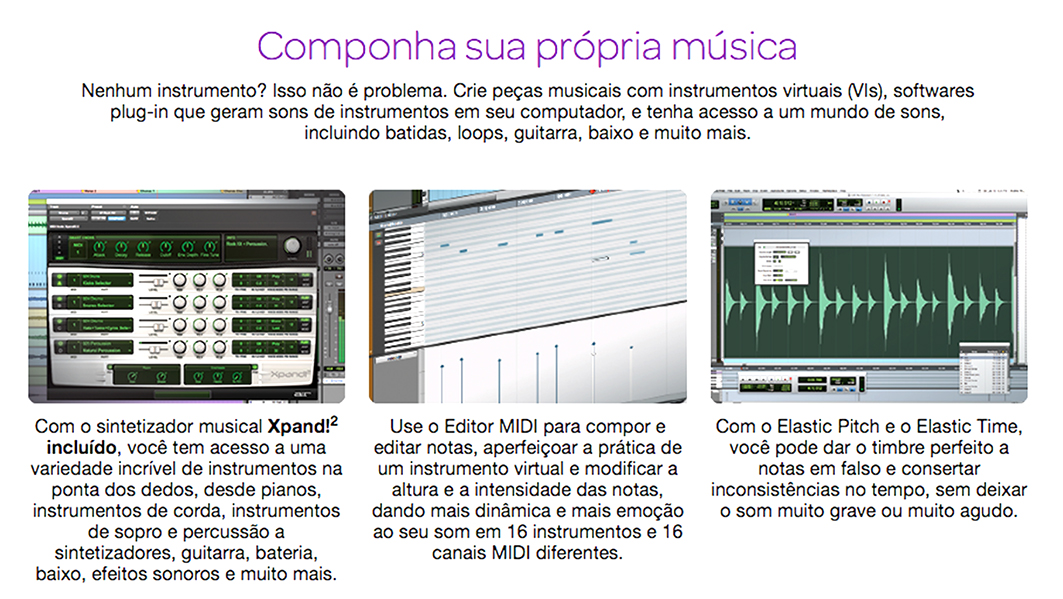
\includegraphics[width=0.8\linewidth]{pictures/protools}
        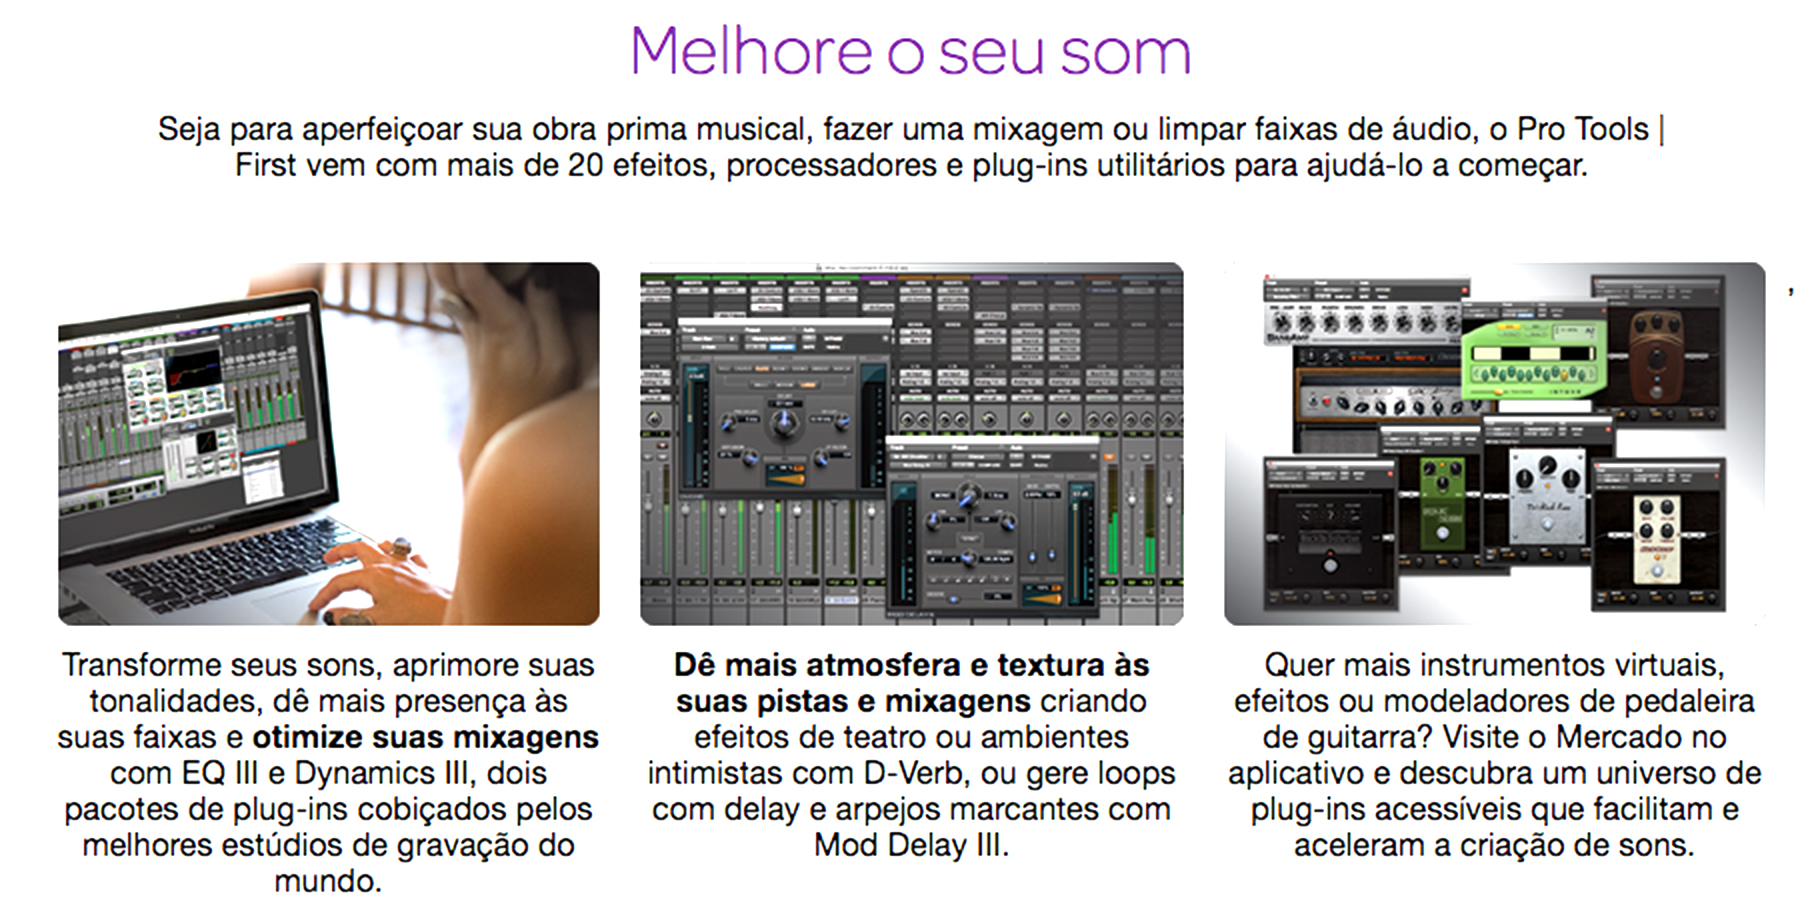
\includegraphics[width=0.8\linewidth]{pictures/protools2}
    
    \legend{Fonte: Print Screen da Autora em 17 de dezembro de 2015. Site: https://www.avid.com/pro-tools-first}
\end{figure}

Outro paradigma de software voltado para produção musical é o dos programas que permitem ao usuário o design de seus próprios aplicativos, como o Pd e o Max. Em 1986, Miller Puckette estava no IRCAM desenvolvendo um software chamado Patcher (um sistema gráfico para produção musical em tempo real para controlar a configurações de objetos no sistema MAX – um ambiente de programação orientada a objetos baseado em janelas voltado para produção musical, que na época rodava em um Macintosh, mas que já rodava no Synclavier II). O Patcher criava um sistema gráfico que simulava o sistema de cabos dos sintetizadores analógicos (figura \ref{analogicos}) e mecanismos de abstração que permitiam condensar módulos criando entradas e saídas que poderiam ser conectadas entre si. Tratava-se na visão de Puckette, um sistema que permitiria que ``os músicos escolhessem dentro de uma ampla gama de possibilidade, desenhando diagramas de fluxo de mensagem" \footnote{\cite[p. 5]{PucketteMiller}}. 

\begin{figure}
    \caption{\label{patcher}À esquerda, um exemplo de patch feito no software Patcher de 1988, e à direita, objetos pré-programados e elementos de controle para configuração da interface gráfica.}
    
        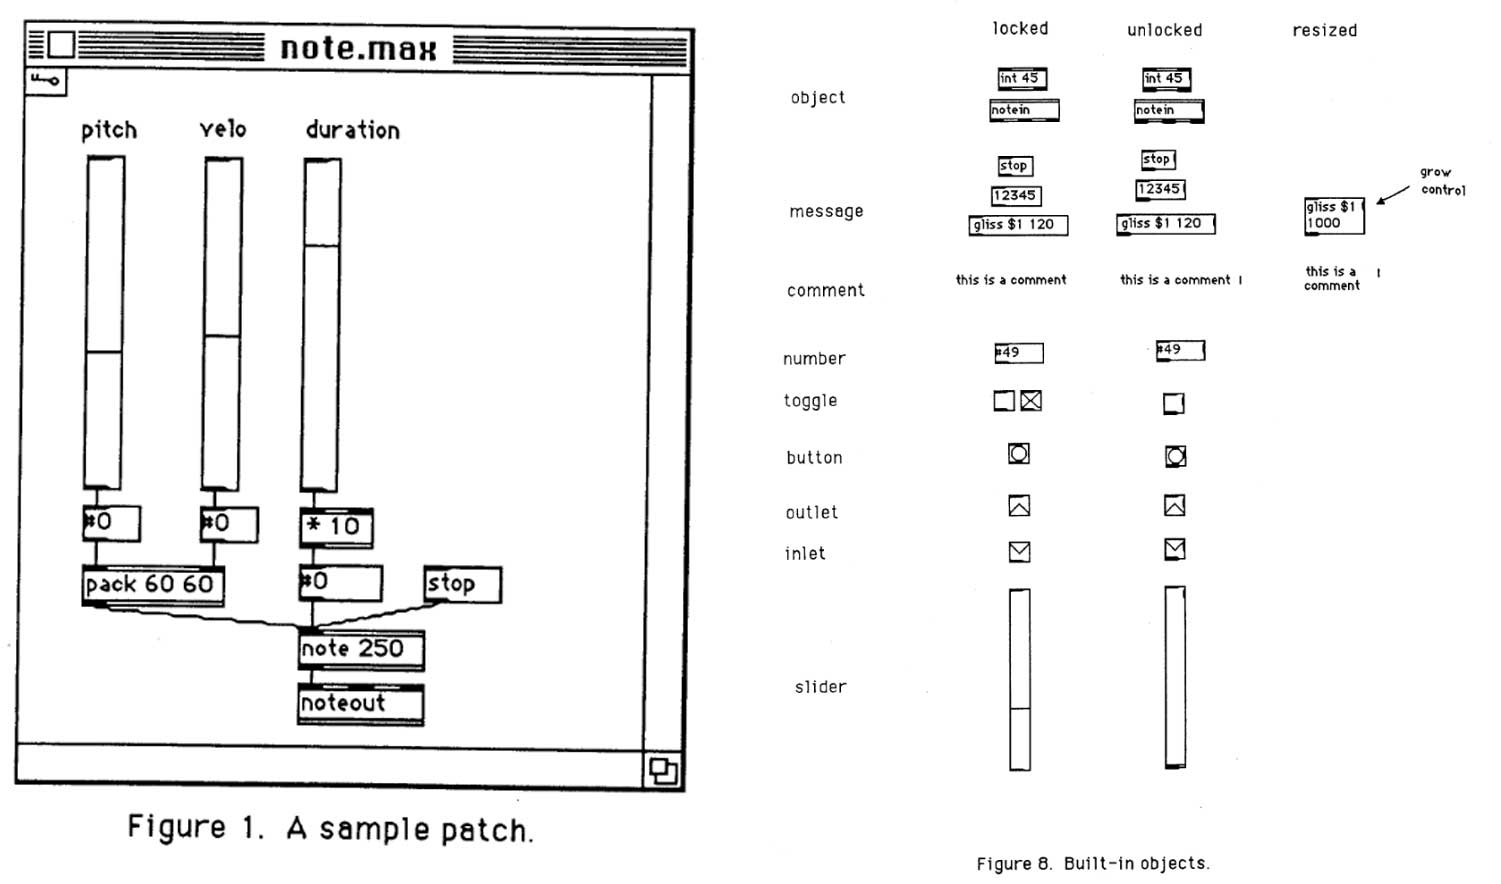
\includegraphics[width=1\linewidth]{pictures/cap2/patcher}
    
    \legend{Fonte: \cite[p. 6,9]{PucketteMiller}}
\end{figure}


Em 1990 o Patcher foi licenciado à Opcode e foi comercializado como Max\/Opcode, passando a ser desenvolvido por David Zicarelli. Em meados dos anos 90 a produção do software foi descontinuada pela Opcode, enquanto Miller Puckette continuou o desenvolvimento do programa no IRCAM que levou ao Max\/FTS (Faster than sound). Em 1996, Miller redesenhou totalmente o software e o lançou como um programa gratuito de código aberto chamado Pure Data (Pd), com uma interface gráfica muito semelhante à do Patcher original e das primeiras versões do Max. No ano seguinte, Zicarelli fundou a Cycling 74, que continuou o desenvolvimento e comercialização do Max\/MSP (abreviação tanto de Max Signal Processing ou de Miller S. Puckette) até os dias de hoje como software proprietário \footnote{\cite{Cryer2018}}.


\emph{Patchers}, como o Pd e o Max, podem permitir a construção de interfaces complexas e adaptadas para necessidades específicas de músicos e artistas, mas possuem uma linguagem mais complexa e exigem um conhecimento especializado de quem as programa. O Pd é, de uma certa forma, uma metáfora de ``bancada para o design de instrumentos musicais eletrônicos para performance musical ao vivo", com objetos pré programados que podem ser conectados para que os artistas criem seus próprios instrumentos de acordo com necessidades específicas. \footnote{\cite{PucketteMiller}}
 
Por mais que programas como \emph{patchers} sejam tentativas de prover o músico com um leque ampliado de potencialidaes criativas, as ferramentas  são em geral também formas de restrição das potencialidades musicais, como aponta Puckette (\citeyear{PucketteMiller}):

\begin{citacao}
 O desenvolvedor de software se esforça para impor o mínimo de restrições estilísticas possíveis sobre o musicista. No entanto, toda nova geração de software que surge revela possibilidades que, de alguma forma, não foram possíveis, ou pelo menos não encorajadas, pela geração anterior. Logo iremos aprender que, não importa o quão generosos ou poderosos sejam os softwares atuais, eles estavam de fato impregnados de suposições tácitas sobre como fazer música que restringem o campo das possibilidades musicais.

%Musicians can’t do much today without software, and so they are dependent on software developers. Software developers in turn are dependent on “users” (the musicians) to make artistic creations with their software; without that, the work of software development is pointless. The software developer strives to impose as few stylistic restrictions as possible on the musician. Yet every new generation of software that comes along reveals possibilities that were somehow not made possible, or at least not encouraged, by the previous generation. Soon we will learn that, no matter how general and powerful we believe today’s software to be, it was in fact steeped in tacit assumptions about music making that restrict the field of musical possibility. \footnote{\cite{PucketteMiller}}
\end{citacao}

%Complexity is not the same thing as expressive power. One wants one’s software to have the greatest expressive power possible, in the simplest possible way. \cite{PucketteMiller}

%\begin{citacao}
%There is also a more subtle, and perhaps more fundamental, aim: to make it so that the software doesn’t impose one or another stylistic bias on the musician. Such a bias might be easy to spot (a built-in set of available time signatures or musical scales, for instance), or might be so ingrained as to be almost invisible (for example, Max’s and Pd’s orientation toward reactivity that seems to privilege some approaches to real-time performance over others).
%\end{citacao}

\subsubsection{New Interfaces for Music Expression}


%\todo[inline]{outras práticas da comunidade NIME} 

Existe no meio acadêmico um volume expressivo de trabalhos e artigos que tratam das capacidades e de aspectos mais técnicos da computação musical, como o livro de Dan Hosken, ``Introduction to Music Technology'' (2011) e as publicações de Curtis Roads Computer ``Music Tutorial'' (1996) e Foundations do Computer Music (1985), ou sobre história da computação musical, como o trabalho de Thom Holmes, ``Electronic and Experimental Music: Technology, Music, and Culture'', (1985), mas provavelmente, o maior volume de pesquisa no campo da interface para produção musical é no desenvolvimento do que chamamos de ``NIME''. 

Em 2001, um grupo de pesquisadores propôs para a conferência CHI (Conference on Human Factors in Computing Systems), uma das mais importantes conferências em estudos do campo de interação humano computador (IHC) um workshop sobre ``New Interfaces for Music Expression'', embasados no rápido desenvolvimento das novas tecnologias digitais e eletrônicas, que estavam trazendo novas potencialidades para o campo de pesquisa de tecnologia musical. Entre seus objetivos estavam pesquisar e discutir o estado atual de ferramentas de controle para performance musical; identificar questões relacionadas entre mudanças de tecnologias e mudanças nas formas musicais; identificar como controles alternativos afetavam a expressão musical e o processo criativo de uma maneira geral e reunir experiências de trabalhos e estratégias dos participantes para resolver questões da área\footnote{\cite{Poupyrev2001}}. Depois deste primeiro \emph{workshop}, NIME se tornou uma conferência própria, que acontece anualmente reunindo diversos trabalhos de pesquisa e desenvolvimento de interfaces experimentais --- físicas ou digitais. 


Overholt (2009), quando define o ``espaço do design das tecnologias de interfaces musicais'', foca na questão do mapeamento e categorização dos gestos, que é uma posição mais ligada à ergonomia. O pesquisador Marcelo Wanderley, da universidade McGill, é um dos que vêm pesquisando a questão do mapeamento do gesto musical em novas interfaces para computação musical, no livro ``New Digital Instruments: control and interaction Beyond the keyborad'', escrito em conjunto com Eduardo Reck Miranda, eles tratam de diversas abordagens desenvolvidas nos últimos anos nesse sentido, como captura de gestos através de câmeras ou dispositivos baseados em sensores e software\footnote{\cite[p. 67]{Miranda2006}}. 

%cultura digital potencializou pesquisa em NIME

O compositor Eduardo Reck Miranda, que também é um dos cientistas brasileiros com produção mais significativa no NIME, desenvolve pesquisa de ponta na área de tecnologia musical, com estudos que incluem o uso de inteligência artificial para composição musical, por exemplo, no trabalho ``Caossynth'' \citeyear{Miranda2016}, e também têm explorado o uso de ciência biomolecular em composições mais recentes como ``DNA: Artibiotics'' \citeyear{miranda2018artibiotics}, que utiliza moléculas de DNA sintetizadas como agentes para composição musical.


Muito do trabalho desenvolvido no campo dessas novas interfaces, no entanto, é direcionado a um músico virtuoso, com grande domínio de técnicas musicais, como aponta Yina Blaine, uma das propositoras do primeiro workshop NIME de 2001:

\begin{citacao}
Talvez como um reflexo da visão Ocidental dominante de que música deva ser tocada apenas por músicos, a maioria dos trabalhos utilizando novas interfaces para expressão musical dos últimos trinta anos é orientada principalmente para experiências e performances virtuosísticas. Com intrumentos em estilo virtuoso, o designer pode rasoalvelmente esperar que o musicista vá investir uma quantidade tempo significativa em aprender as idiossincrasias do instrumento.
%Perhaps as a reflection of the dominant Western view that music should be played only by musicians, most work in the last thirty years using new interfaces for musical expression is primarily oriented toward virtuosic experiences and performances. With virtuoso-style instruments, the designer can reasonably expect the player to invest a significant amount of time learning the idiosyncrasies of the instrument. \cite{Blaine2003}
\end{citacao}



\subsubsection{Experiências em Web Audio}
Enquanto as produções em NIME costumam ser dedicadas à musicos virtuosos ou com grande nível de conhecimento técnico, exite também um campo de pesquisa em música ubíqua (UBIMUS)\footnote{\cite{Keller}}, que procura desenvolver ferramentas para o suporte criativo de atividades musicais para um grupo maior de pessoas, devido às possibilidades ampliadas de acesso oferecidas pelas tecnologias de rede e dispositivos móveis, ou nas palavras de Pimenta, Keller e Lazarini (\citeyear{Keller}):

\begin{citacao}
Um dos nossos objetivos é o de desenvolver ferramentas que tirem vantage desse contexto inclusivo, provendo condições para que noviços interessados em música participem de atividades criativas, em qualquer lugar e em qualquer momento, usando os dispositivos convencionais de comunicação móvel ou de computação que eles já possuam, e sejam familiares. \cite[p. 13]{Keller}

\end{citacao}

%One of our goals is to develop tools which take advantage of these inclusive contexts, providing conditions to novices interested in music to participate in creative activities, in any place and at any moment, using the very conventional mobile communications and computing devices that they already own, and are familiar

Quando inciamos essa pesquisa, já haviam alguns produtos de programação criativa disponíveis que estavam explorando esses novos recursos de Web Audio como suporte. Como forma de sistematizar a pesquisa, fizemos um levantamento de experimentos organizados pelo site ``Chrome Experiments'' que reúne milhares de casos de uso produzidos pela comunidade de ``programação criativa''\footnote{Disponível na url: \url{https://experiments.withgoogle.com/experiments}}. Em julho de 2016, apenas na categoria ``Sound and Music''  haviam listados 138 experimentos, desses uma série deles são experimentos estéticos com música generativa, jogos sonoros, videoclipes interativos, visualizadores de áudio, mixers e tocadores de MIDI, e alguns podiam ser considerados instrumentos musicais. Entre eles encontramos vários exemplos de sintetizadores, \emph{samplers}, processadores de áudio e sequenciadores, mas a maioria deles tinha como interface algo que mimetizam algum instrumento analógico ou eletrônico, principalmente o piano.

Encontrei algumas possibilidades interessantes como as experiências ``Lalo.li'' \footnote{Disponível em: <http://lalo.li/> }, que faz síntese de voz a partir de texto digitado na tela, podendo o usuário mudar o tom e a velocidade da voz. Sua interface é pareceida com a de um sistema de busca, bastante minimalista, com um input de texto e os controles para alterçnao dos parIametros de síntese.

\begin{figure}
    \caption{\label{laloli}Interface do site Lalo.li.}
    
        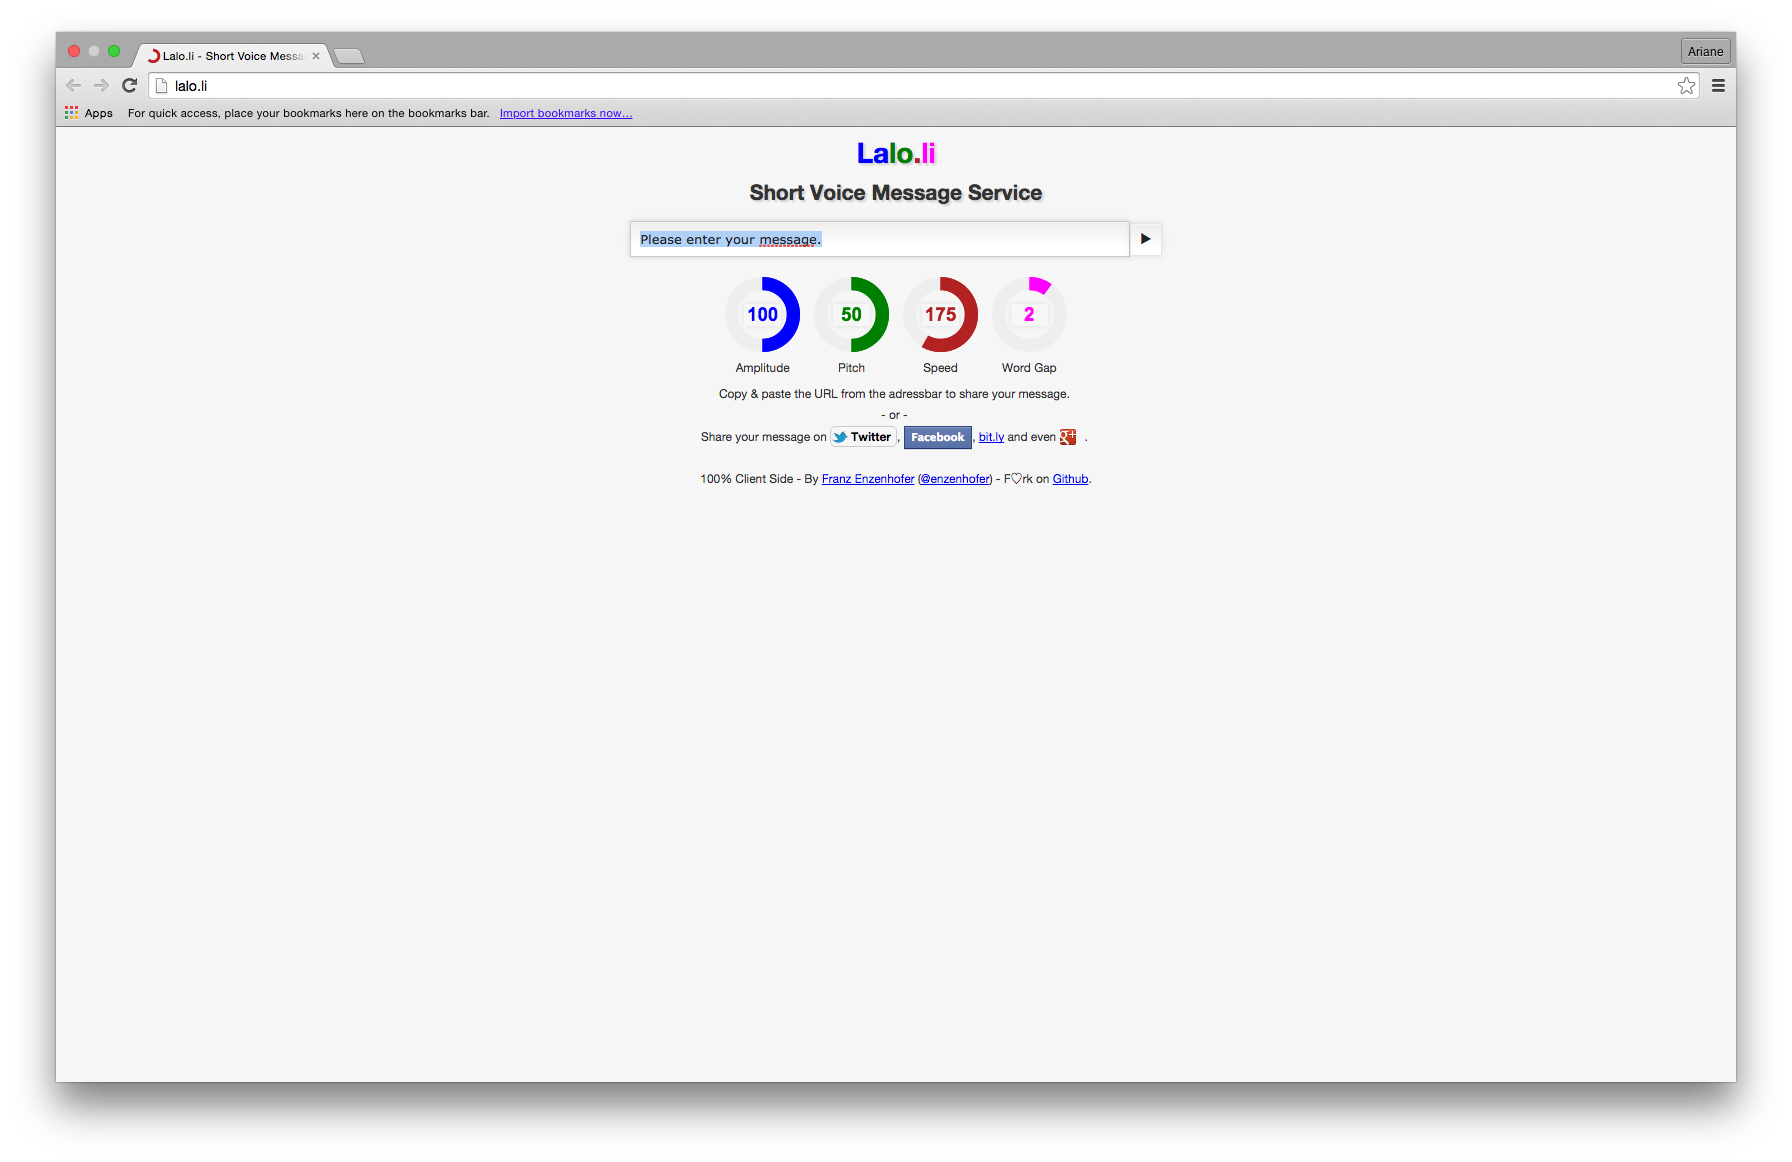
\includegraphics[width=1\linewidth]{pictures/cap2/laloli}
    
    \legend{Fonte: Screenshot da autora, dia 15 de março de 2016}
\end{figure}

O ``Spectrogram and Oscillator''\footnote{Disponível em: <http://smus.com/spectrogram-and-oscillator/>} (Figura \ref{spectrogramosc}) desenha um gráfico do espectro das frequências do som em tempo real a partir da entrada do microfone ou de um oscilador por clique. Esse experimento foi bastante interssante pois mostrou a executabilidade da análise por FFT em tempo real a partir do navegador. O sistema de síntese embutido, no entanto é bastante limitado, resumindo-se apenas a um oscilador simples.   



\begin{figure}
    \caption{\label{spectrogramosc}Interface do Spectrogram and Oscillator.}
    
        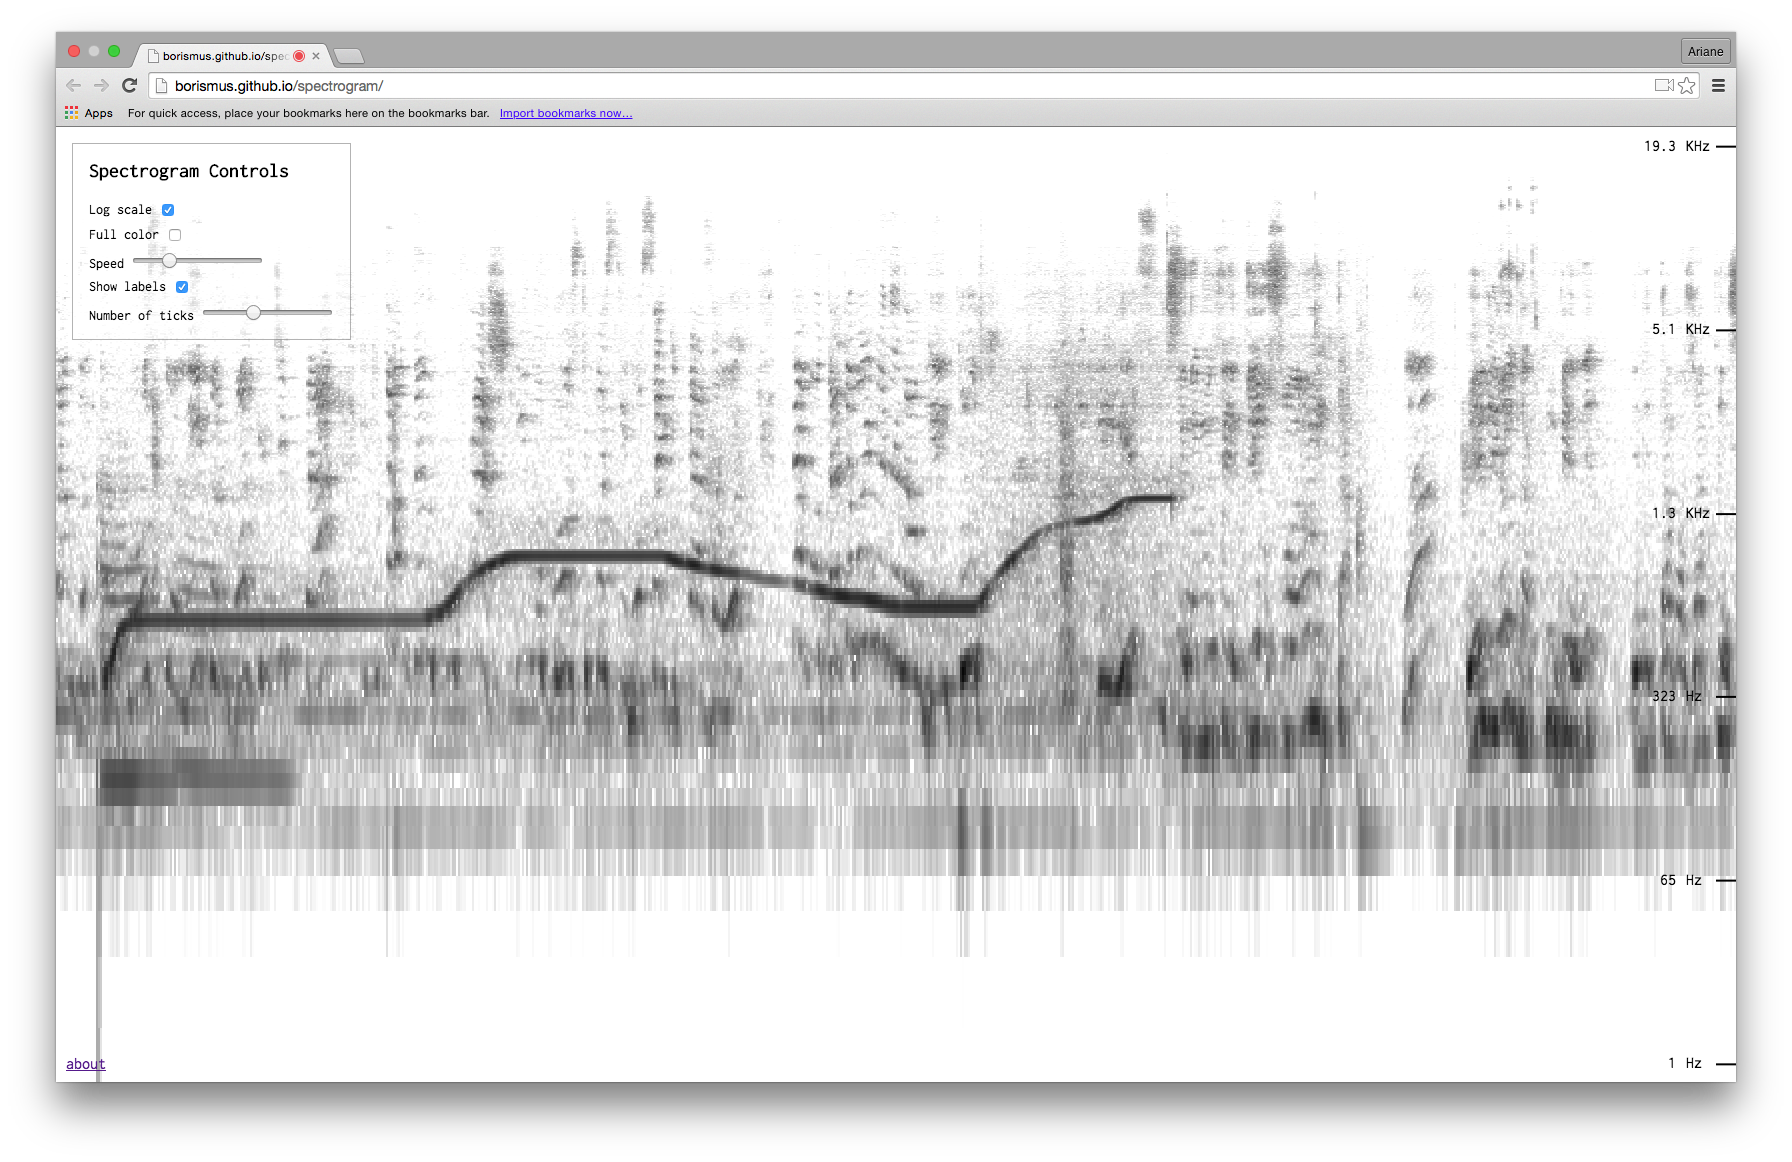
\includegraphics[width=1\linewidth]{pictures/cap2/spectrogramandoscilator}
    
    \legend{Fonte: Screenshot da autora, dia 15 de março de 2016}
\end{figure}

Patatap\footnote{Disponível em: \url{http://patatap.com}} é uma espécie de bateria eletrônica audiovisual (Figura \ref{patatap}), que usa o teclado como input. O sistema apresenta uma co-relação entre som e gráficos gerados em SVG. A quantidade de sons, no entanto, é limitada à quantidade de teclas do teclado. Os sons são fixos, e não é possível alterá-los.

\begin{figure}
    \caption{\label{patatap}Interface do Patatap.}
    
        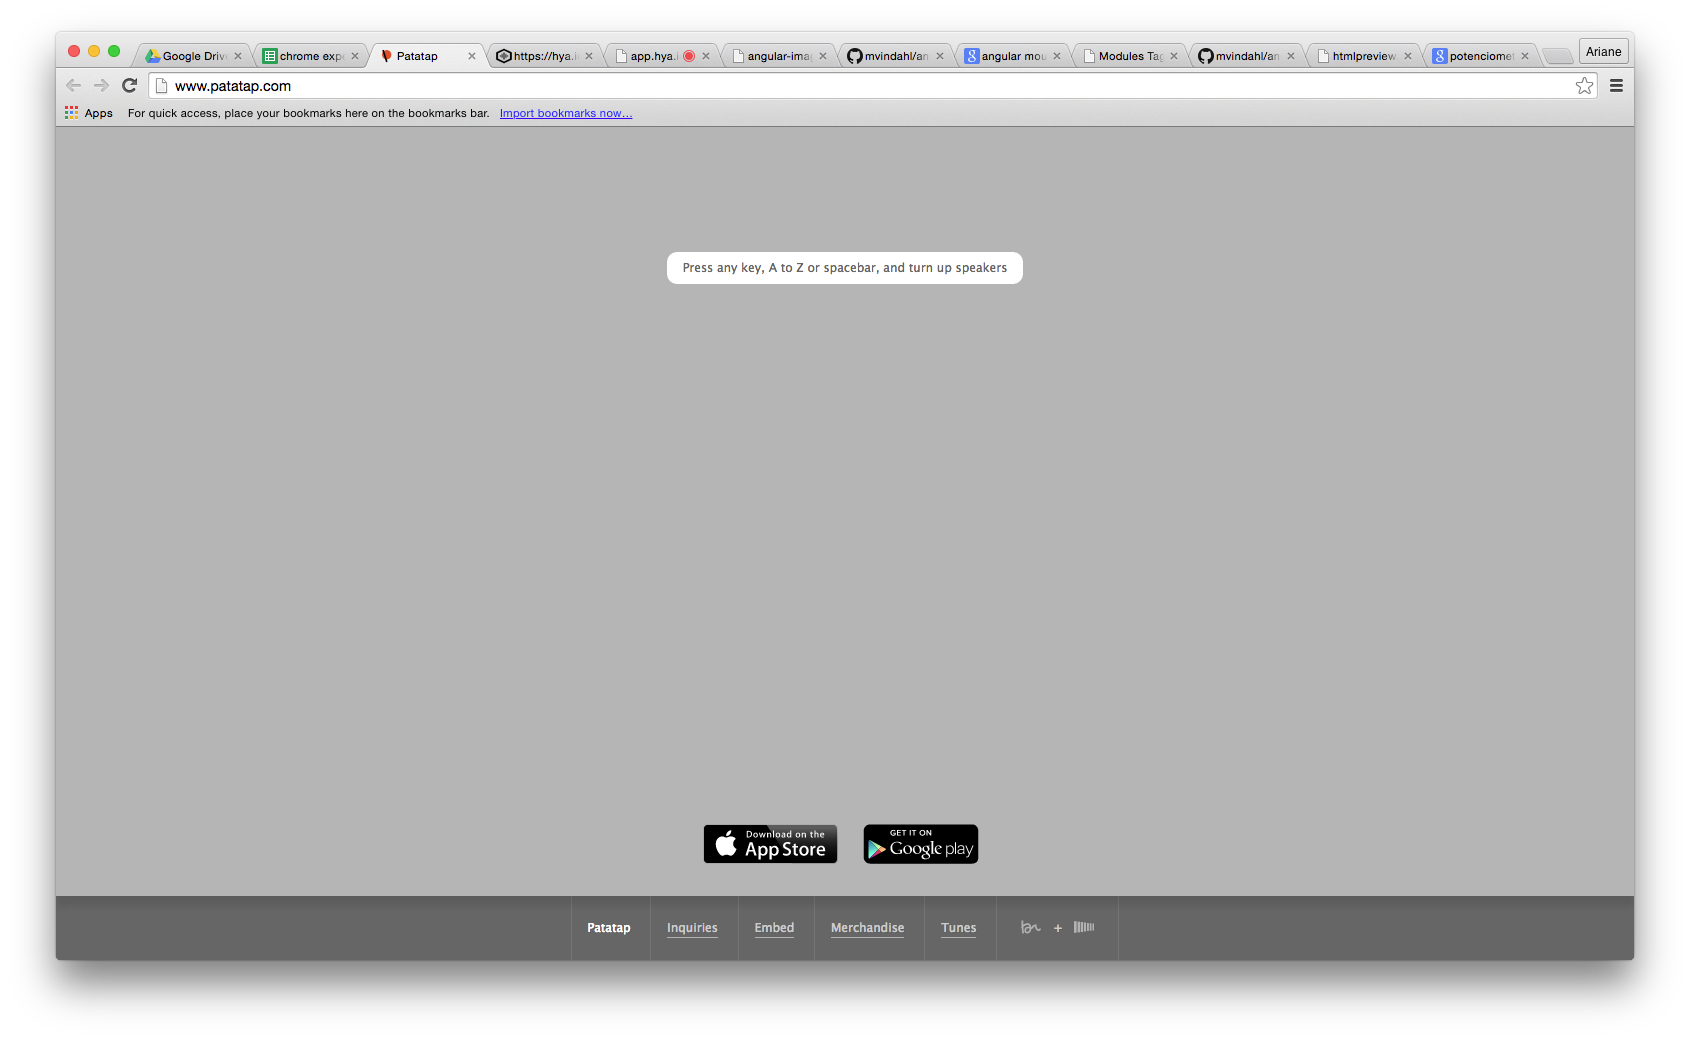
\includegraphics[width=1\linewidth]{pictures/cap2/patatap}
    
    \legend{Fonte: Screenshot da autora, dia 15 de março de 2016}
\end{figure}

Especialmente interessantes para o contexto dessa pesquisa são alguns experimentos multiusuário como o ``Plink'' (Figura \ref{plink}), onde cada pessoa que entra no site controlava um ``instrumento'' que se podia tocar com o mouse a partir de faixas verticais que representavam notas diferentes. O experimento, que não está mais no ar, tinha uma grade de tempo fixa, e os usuários que acessavam o site podiam tocar em conjunto a partir de uma lista de opções de timbres diferentes. Os instrumentos eram fixos e as notas também, e não havia possibilidade de trocar a velocidade nem alterar os timbres deles. 

\begin{figure}
    \caption{\label{plink}Interface do Plink.}
    
        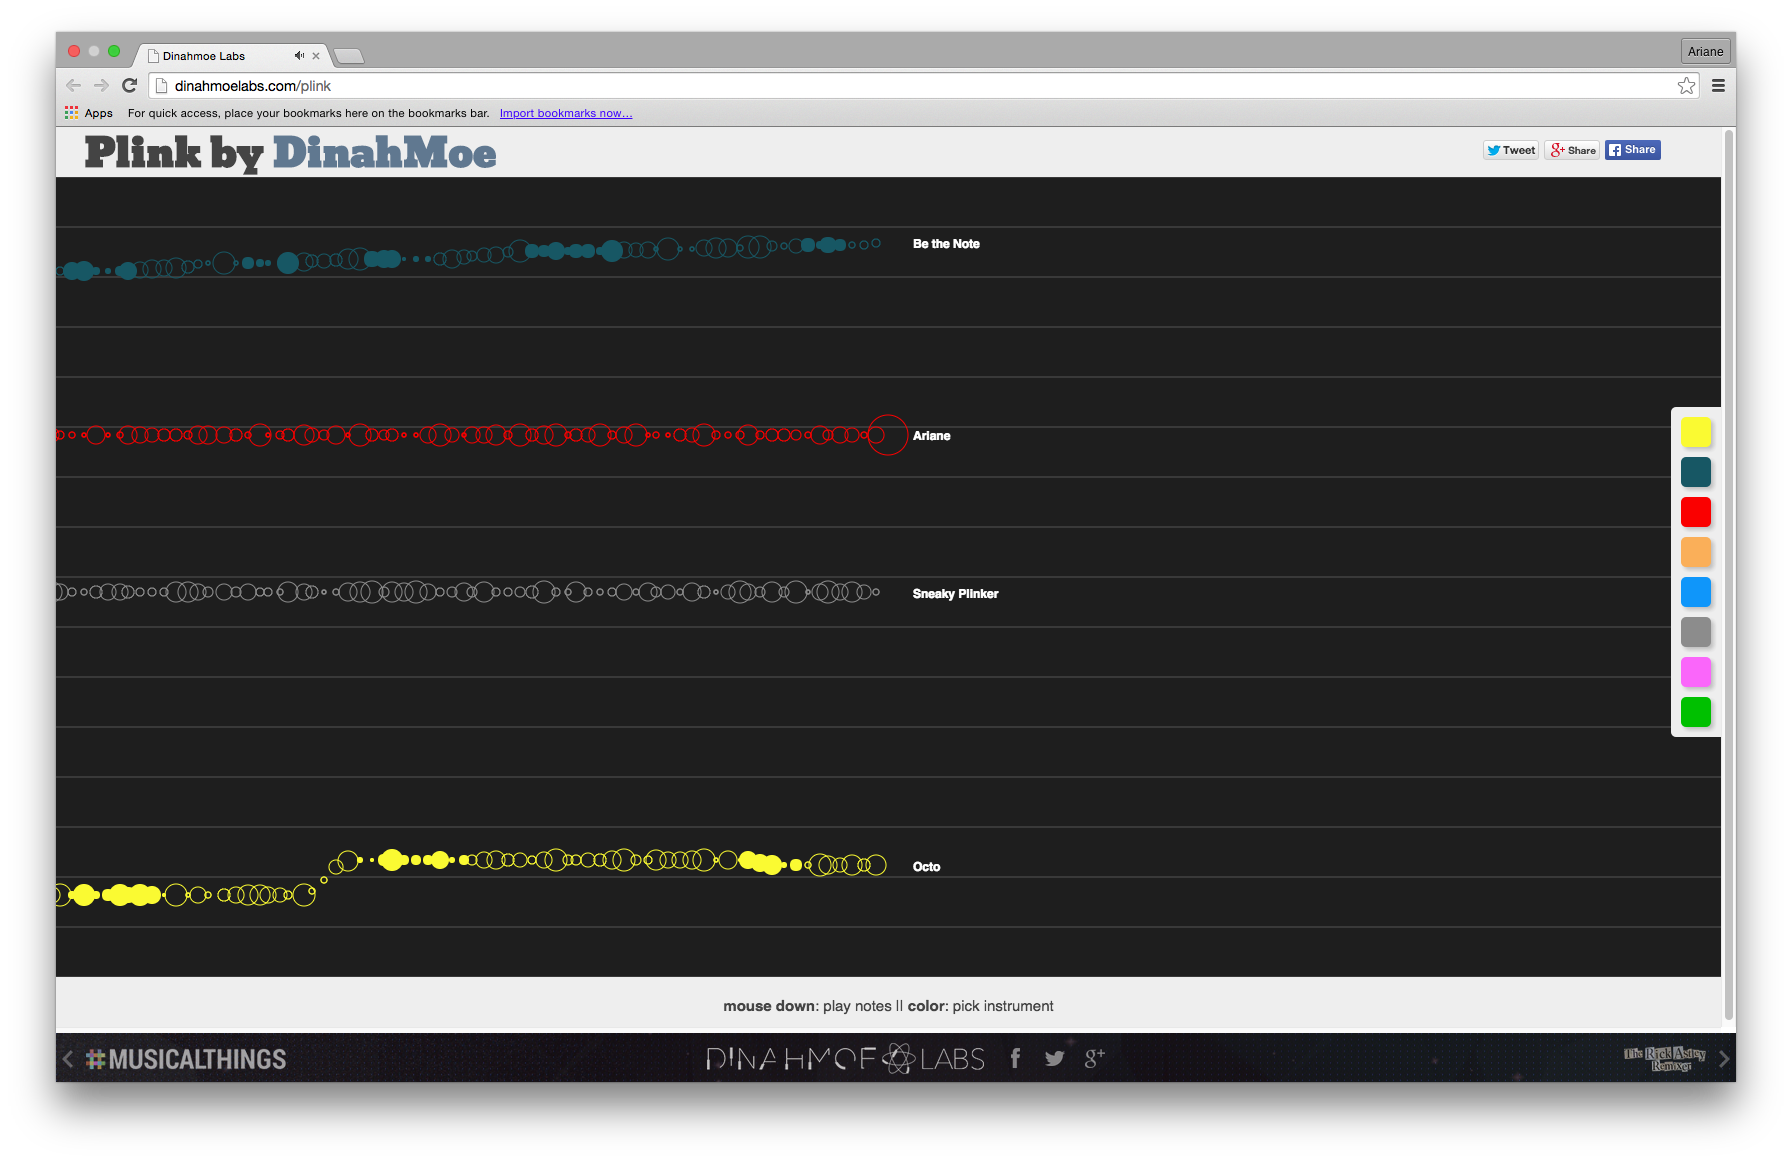
\includegraphics[width=1\linewidth]{pictures/cap2/plink}
    
    \legend{Fonte: Screenshot da autora, dia 15 de março de 2016}
\end{figure}

O ``Multiplayer Piano''\footnote{Disponível em: http://www.multiplayerpiano.com/} (Figura \ref{multiplayer}), é um piano \emph{online} aberto, onde os usuários do site se encontram virtualmente e podem tocar em conjunto. Cada usuário \emph{online} é representado por um cursor que fica circulando pela página. A interface possui um \emph{chat}, onde os usuários conversam em tempo real. Também é possível conectar o site com controladores MIDI, e é possível criar salas virtuais privadas para tocar em grupos menores. Como experiência musical, é bastante interessante, pois é um piano caótico, onde muitos tocam ao mesmo tempo. Como recuso para prática musical, no entanto é limitado, porque se limita aos sons de piano de poucas oitavas. A interface também é bastante tradicional, imitando um teclado na tela.


\begin{figure}
    \caption{\label{multiplayer}Interface do Multiplayer Piano.}
   
        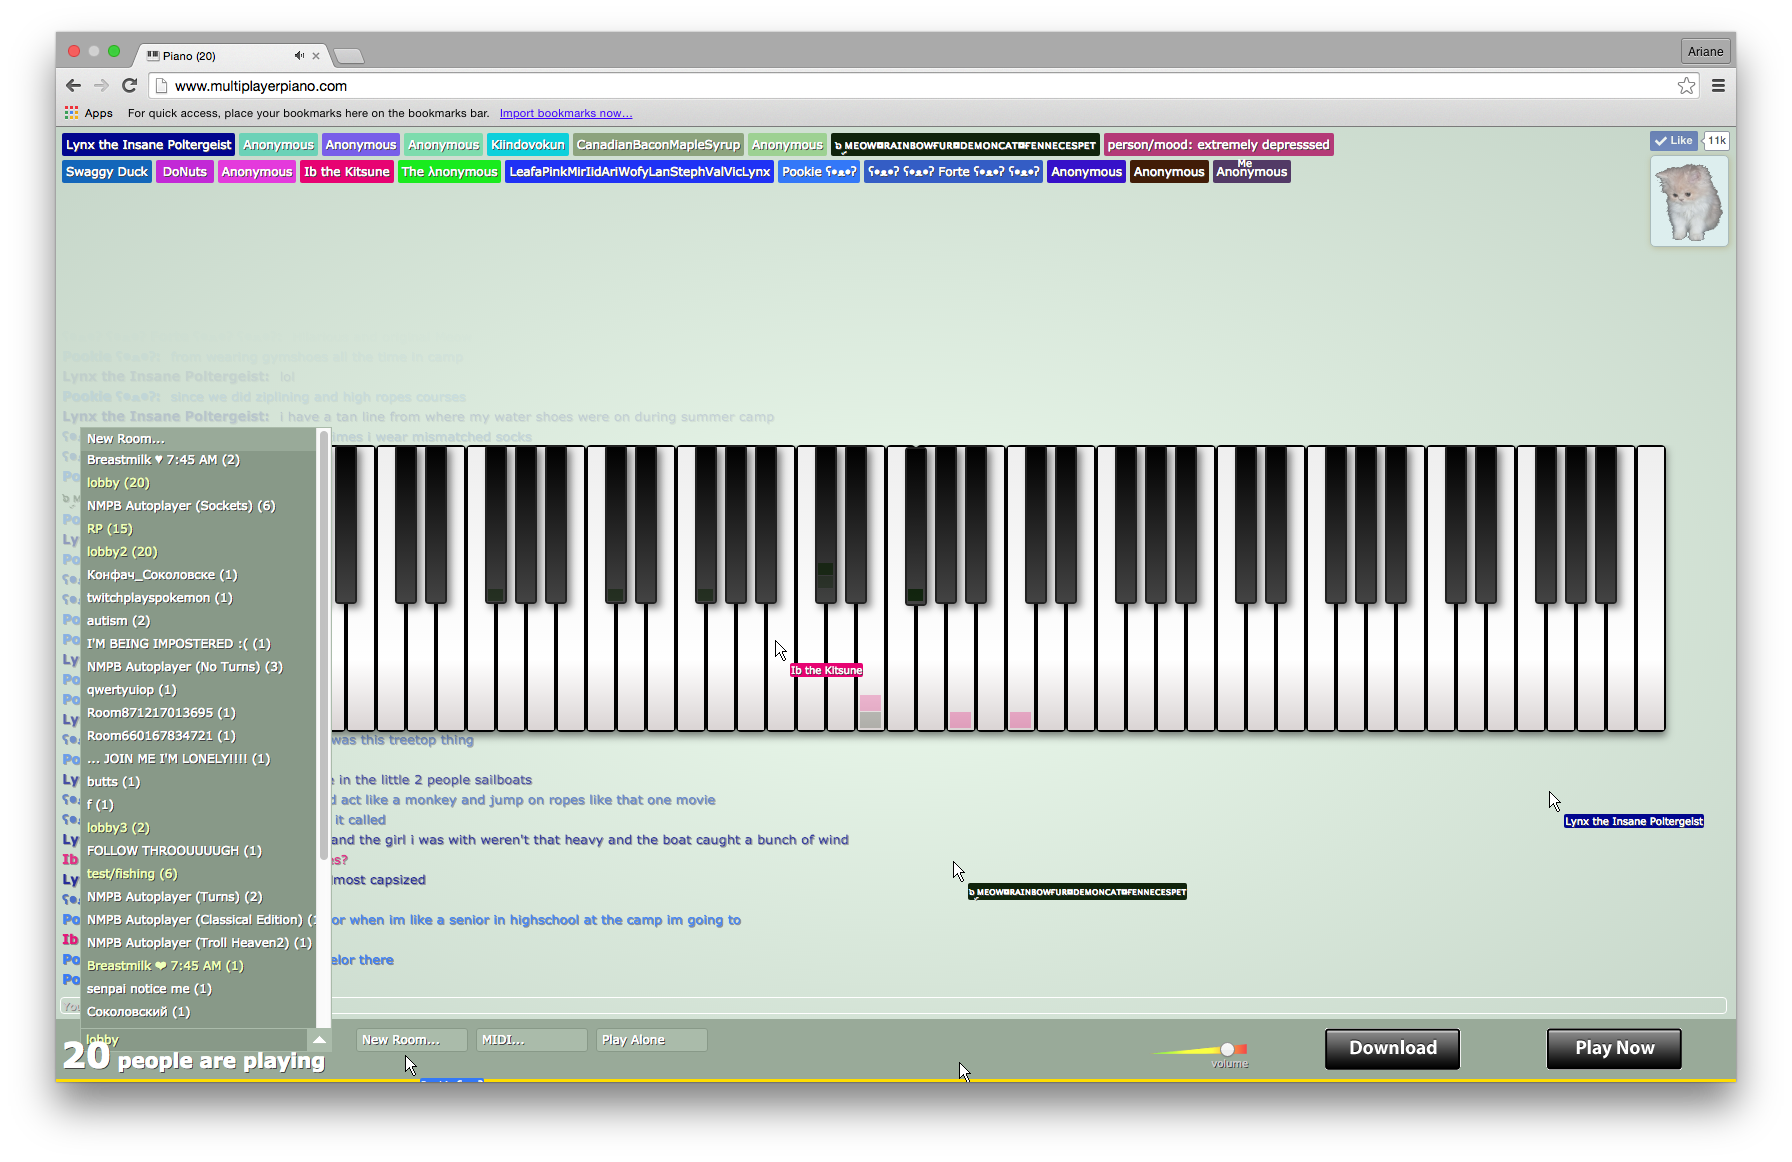
\includegraphics[width=1\linewidth]{pictures/cap2/multiplayerpiano}
   
    \legend{Fonte: Screenshot da autora, dia 15 de março de 2016}
\end{figure}


No Brasil, o projeto música móvel \footnote{\cite{Rohde2014}}, reuniu pesquisadores como Bruno Rohe, Glerm Soares e Cristiano Figueiró para produzir aplicativos de musicais para telas multique em sistema Android e software livre (Figura \ref{mmovel}). Eles usaram como base uma biblioteca que permite criar aplicativos baseados em PureData (libPD). Entre eles, o ``Looper'' \footnote{Vídeo demontrativo disponível em: https://www.youtube.com/watch?v=aTOdMNtC-sA}, que permite gravar loops em diversos canais e aplicar filtros e efeitos no domínio do tempo das frequências; B\/I\/T\/S\/L\/C (beatslicer), que ``construir
recombinações de sequenciamento de fatias de áudio''; o Photosíntese, que trabalha com síntese sonora a partir das informações de cor da imagem da câmera do celular.

\begin{figure}
    \caption{\label{mmovel}À esquerda, interface do programa looper, e à diretita do B\/I\/T\/S\/L\/C, alguns dos aplicativos desenvolvidos pelo projeto Música móvel.}
    
        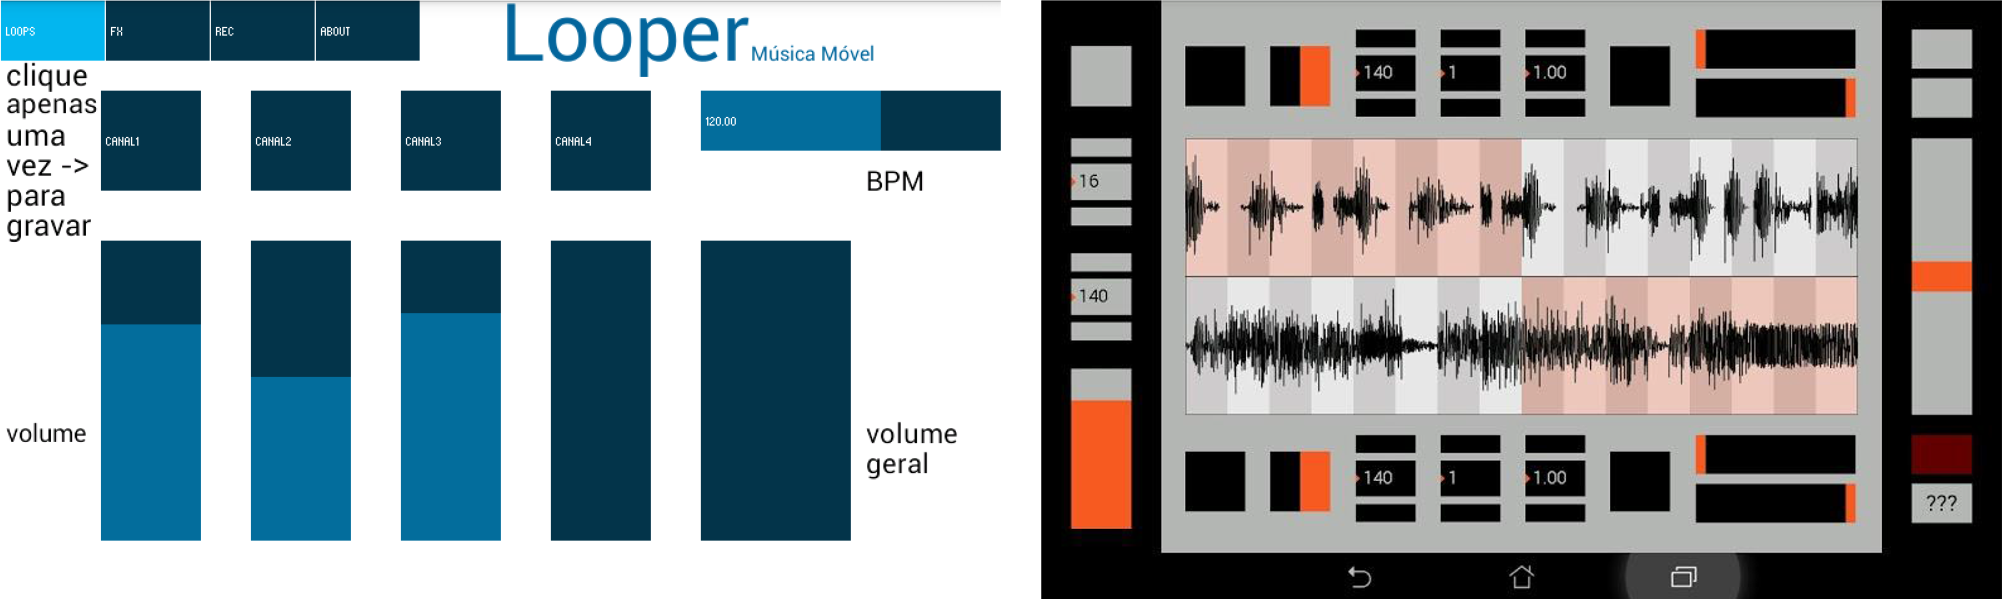
\includegraphics[width=1\linewidth]{pictures/cap2/musicamovel}
    
    \legend{Fonte: \cite{Rohde2014}}
\end{figure}

Em 2016, com a profusão de trabalhos relacionados a tecnologias web e áudio, foi organizada a primerira WebAudioConference, que foi sediada no IRCAM. Entre os tópicos da conferência, estavam: experiências inovadoras em aplicações web para áudio e música; integração multimídia; visualização de áudio nos navegadores; processamento de áudio nos navegadores; hardware e interfaces tangíveis e uso da web audio api e outros temas relacionados à aplicação de tecnologias web para áudio e música\footnote{\url{https://wac.ircam.fr/}}. Nas conferências, que aconteceram anualmente desde 2016, foram apresentados uma série de trabalhos explorando essas tecnologias para produção musical, como emuladores de DAW \footnote{\cite{Jillings2017}} ou sequenciadores \footnote{\cite{Feenstra2016}}. Com os ecperimentos que descrevemos nas próximas seções, tivemos a oportunidade de participar das dúas últimas conferências em Londres (2017) e em Berlim (2018), apresentando a versão em Web Audio do Projeto Banda Aberta\footnote{\cite{Stolfi2017b}} e o Playsound.space\footnote{\cite{Stolfi2018b}}.




%Innovative audio and music based web applications (with social and user experience aspects)
%Client-side audio processing (real-time or non real-time)
%Audio data and metadata formats and network delivery
%Server-side audio processing and client access
%Client-side audio engine and rendering
%Frameworks for audio manipulation
%Web Audio API design and implementation
%Client-side audio visualization
%Multimedia integration
%Web standards and use of standards within audio based web projects 
%Hardware, tangible interface and use of Web Audio API

%\textbf{(ii) Instrumentos musicais online.} Nos últimos anos, principalmente depois do lançamento da Web Audio API, muitas pesquisas têm sido conduzidas no desenvolvimento de plataformas para tocar música na rede. Uma parte delas são baseadas em tipos existentes de instrumentos musicais digitais, 
%\todo{incluir mais referencias aqui}


Essa diversidade de trabalhos demonstra o potencial das tecnologias web para o desenvolvimento de novas interfaces para produção musical, no entanto, a maioria dos instrumentos desenvolvidos até então ou exigiam um conhecimento prévio de técnicas musicais, ou são muitos simples e restritas em termos de expressividade musical\footnote{\cite{Dobrian2006}}, aproximando-se mais da idéia de um jogo musical do que de um instrumento propriamente dito. Apesar de mostraram que existe uma imensa potencialidade latente em explorar essas novas tecnologias, permitindo processos complexos de síntese de áudio e sampleamento, esses experimentos ainda eram relativamente precários em termos de potencialidades de produção musical, se compararmos às ferramentas disponíveis para produção musical em software, como os chamados digital audio workstations (DAW) ou os \emph{patchers}.



% !TEX encoding = UTF-8 Unicode
% !TEX root = tese.tex


\chapter{Experimentos}
\label{ch:experimentos}


\section{Primeiros Experimentos}
Partindo desta pesquisa inicial de referências, procurei começar a desenvolver de fato alguns experimentos práticos voltados à música.  De um lado, tinham as tecnologias de programação, que estavam surgindo naquele momento, mas também havia um repertório e teorias da música que se colocavam com o ingresso no Doutorado. Esses primeiros estudos que foram projetos bastante simples foram importantes como exercícios estéticos e para começar um aprendizado dessas novas tecnologias.


\subsection{Bandas Críticas}
Bandas Críticas pode ser considerada a primeira ``peça'' musical que escrevi. Até então, fazia apenas ``música''. Foi um primeiro exercício de escrita de uma partitura gráfica e de composição para uma equipe tocar. A peça foi composta a partir da proposta apresentada pelo Estúdio Fita Crepe \footnote{O Estúdio Fita Crepe foi um espaço dedicado à produção e performance de música experimental na cidade de São Paulo. \url{http://www.estudiofitacrepesp.com/}} de através do músico Ricardo Garcia ao NuSom, de um concerto de ``Música Silenciosa'', que seria uma ``música para acariciar os ouvidos'', embasada em sutilezas de timbres e volumes.

A proposta foi de explorar metalinguisticamente o conceito de ``bandas críticas'' da audição, como apontamos em uma proposta de apresentação para o Simpósio Brasileiro de Computação Musical de 2015, que ocorreu em Campinas:


\begin{citacao}
A peça explora as frequências centrais e limítrofes das bandas críticas da audição, sobrepondo harmônicos e criando dissonâncias a partir de sons fora das escalas musicais tradicionais. Surge de um processo de composição metalinguístico, de investigar a própria percepção acústica, em um desejo de materialização de conceitos psicoacústicos em objetos sonoros. 
Surge de um processo de composição metalinguístico, de investigar a própria percepção acústica, em um desejo de materialização dos conceitos psicoacústicos em objetos sonoros. No caso, representa uma materialização do conceito de bandas críticas, buscando explorar sensações audíveis e artefatos emergentes da exploração desse conceito. A performance é programada para 3 músicos, cada um conectado a uma caixa de som diferente, para enfatizar as diferenças entre as frequências exploradas. \footnote{\cite{ArianeStolfi2015}}
\end{citacao}

Também foi uma experiência de composição abstrata, a partida da idéia de buscar uma saturação sensória formada a partir de frequências puras, mas não necessariamente harmônicas, que fosse estimular todas as regiões da cóclea. A peça é estruturada em quatro partes, um primeiro movimento introdutório onde os músicos não performam e o processamento acontece de forma automatizada por um \emph{patch} de PD (Figura \ref{bandaspatch}), com todos os 44 osciladores ligando em um volume ascendente; um segundo momento, os músicos vão desligando os osciladores de acordo com uma ordem pré-estabelecidas, causando uma rarefação, até restarem apenas poucos osciladores ligados; na terceira parte os músicos improvisam a partir de harmônicos desses osciladores ligados; por fim, há um momento de ``destruição da onda'', onde os músicos passam a improvisar desenhando a onda, o que gera uma harmonia de ruídos, até a destruição completa dessas harmonias com a busca do silêncio.

\begin{figure}[htb]
    \caption{\label{bandaspartitura}Partitura gráfica para a peça Bandas Criticas. }
    \begin{center}
    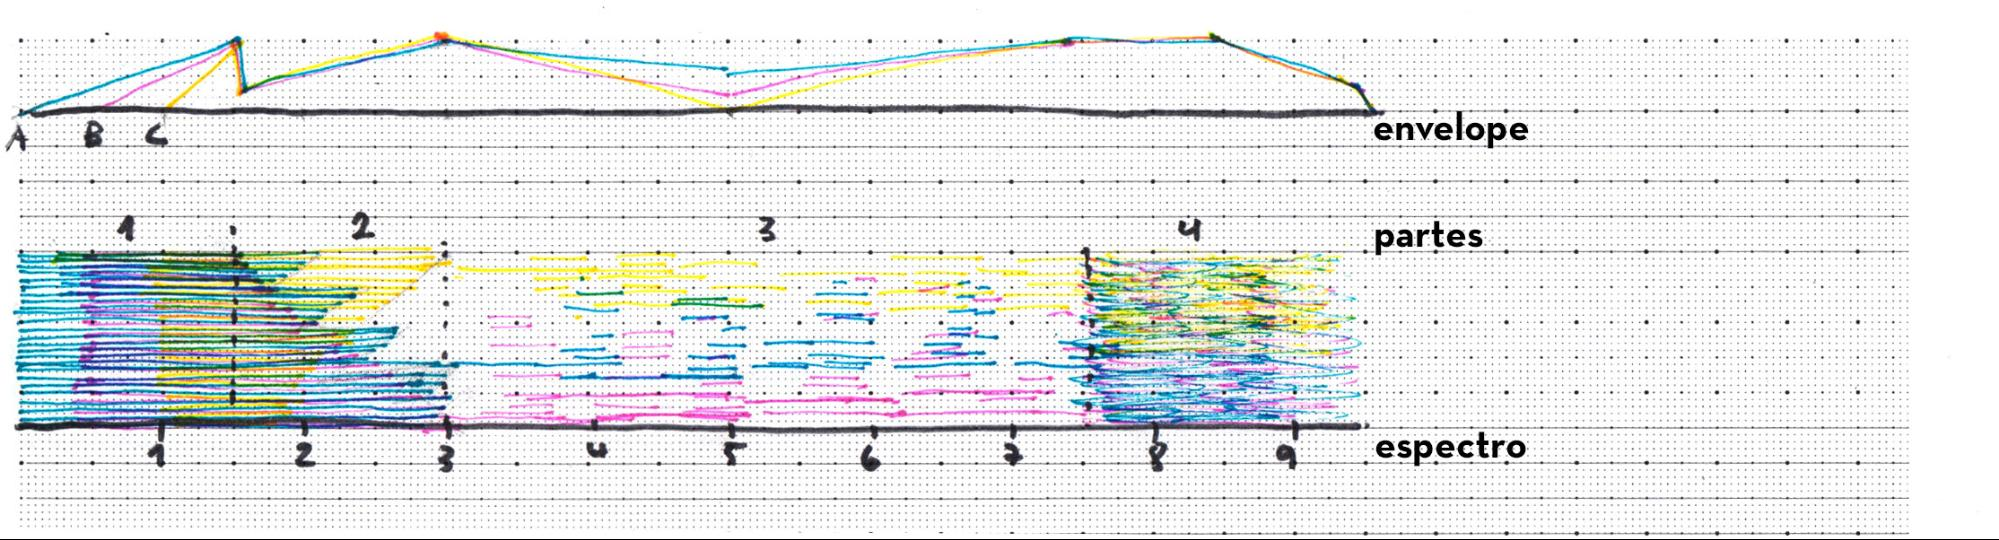
\includegraphics[width=1\linewidth]{pictures/cap3/bandascriticaspartitura}
    \end{center}
    \legend{Fonte: Screenshot da autora, Janeiro de 2016}
\end{figure}

Fizemos uma apresentação no Estúdio Fita Crepe, no evento ``Música? 11'', onde tocaram comigo Davi Donato e Sérgio Abdalla, no dia 29 de agosto de 2015 e outra no Simpósio Brasileiro de Computação Musical no dia 24 de novembro em Campinas, com a participação de Davi Donato e Luzilei Aliel. Análise do registro das gravações mostraram que o espectrograma da peça ficou bem próximo ao desenho da partitura pensado originalmente, como podemos ver na imagem \ref{bandasciticasspec}. 

\begin{figure}
    \caption{\label{bandaspatch}Patch para a peça Bandas Criticas. }
    \begin{center}
    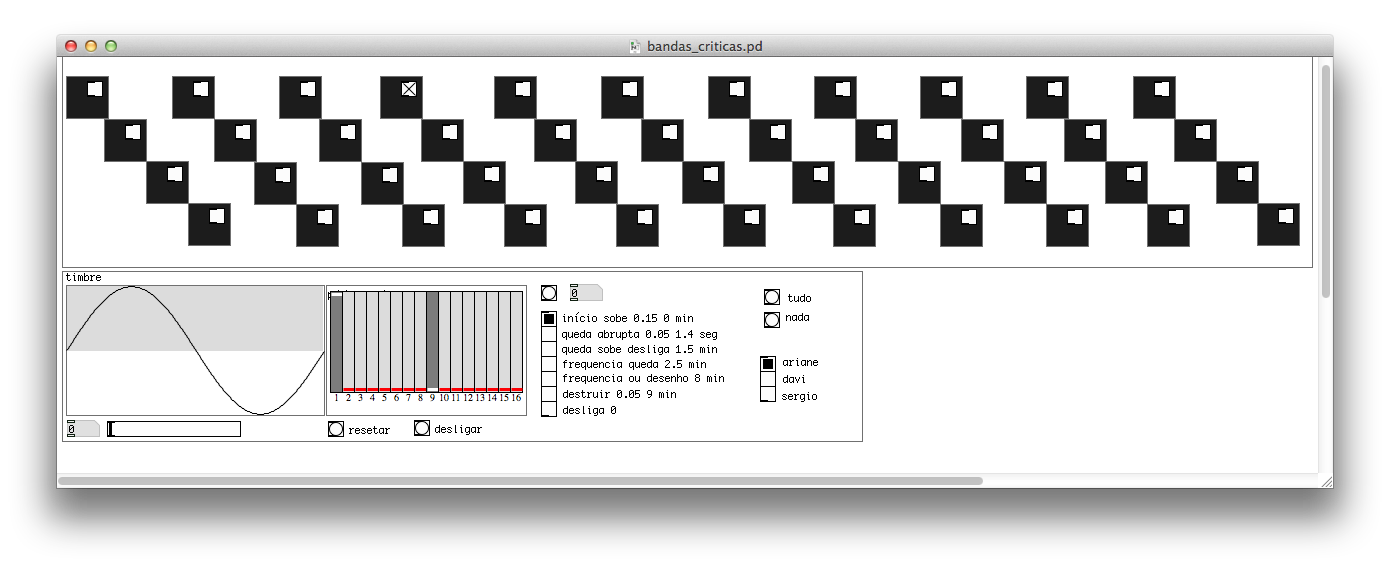
\includegraphics[width=1\linewidth]{pictures/cap3/bandascriticaspd}
    \end{center}
    \legend{Fonte: Screenshot da autora, Janeiro de 2016}
\end{figure}

\begin{figure}
    \caption{\label{bandasciticasspec}Espectrogramas gerados a partir das gravações da peça no Estúdio Fita Crepe (acima) e no SBCM (abaixo). }
    \begin{center}
    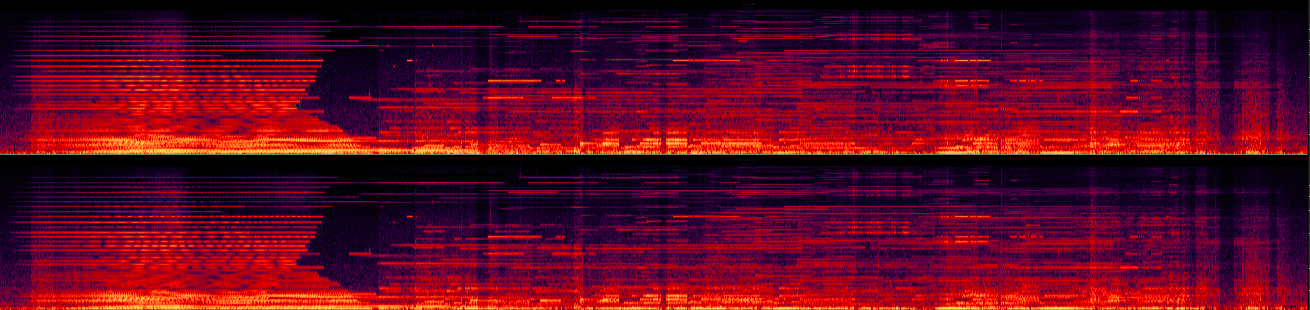
\includegraphics[width=1\linewidth]{pictures/cap3/bandascriticasspectro2}
    \end{center}
    \legend{Fonte: Screenshot da autora, Janeiro de 2016}
\end{figure}



\subsection{QWERTY}
\label{sec:QWERTY}
QWERTY foi o primeiro experimento em web áudio desenvolvido após entrar no programa de doutorado. Como a idéia inicial do projeto era buscar formas de explorar os \emph{inputs} dos computadores pessoais, partimos de uma das  principais formas de entrada que é o teclado QWERTY, que tem a disposição ainda das tradicionais máquinas de escrever. A idéia era transformar o teclado em uma máquina sonora, que não é em si uma coisa nova. O site Patatap, por exemplo, que mencionamos no capítulo anterior, é uma plataforma que funciona dessa maneira. Outro exemplo é o ``Typedrummer'' de Kyle Stetz,\footnote{Disponível em: \url{http://typedrummer.com/}} onde para cada letra há um sample e ao digitar um texto, os sons correspondentes são tocados em loop.


Para essa máquina, me inspirei nas leituras de Haroldo de Campos do seu poema épico Galáxias \footnote{\cite{Campos2004}}, que tem como estrutura um bloco contínuo de frases sinestésicas, sem qualquer tipo de pontuação ou espaçamento. 

Naquele momento, estava envolvida também no projeto de digitalização das revistas de poesia concreta Código \ref{codigo}, da revista de vanguarda lançada em 1973 e editada por Erthos Albino de Souza e Antônio Risério, que contém obras e traduções de vários poetas concretos desta geração. A revista Código, como aponta Augusto de Campos ``acolheu materiais de vanguarda que não encontrariam guarida nas publicações convencionais alternativas" \footnote{\cite{Scandurra2016}}. Para a versão online da revista, programei a interface seguindo uma idéia de design de navegação paratática, ou seja, que permitisse a recombinação e re-montagem dos poemas de acordo com a vontade do leitor. Por conta deste projeto, estava em contato constante com as obras dos poetas desta geração, que serviu de inspiração também para essa pesquisa.

\begin{figure}
    \caption{\label{codigo}Interface do site da digitalização da revista Código. }
    \begin{center}
    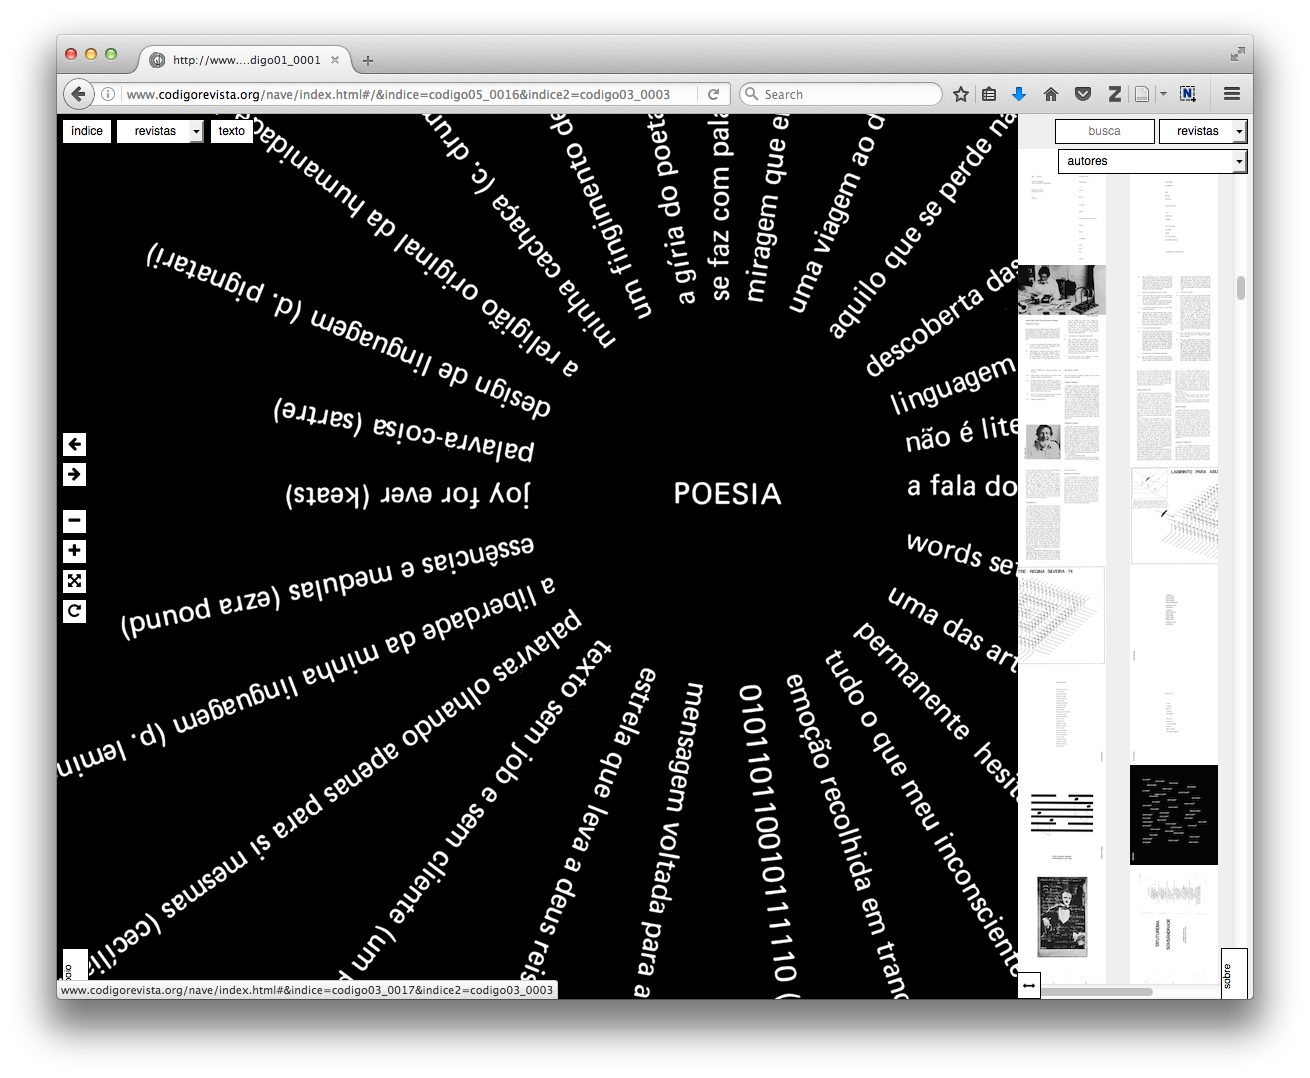
\includegraphics[width=1\linewidth]{pictures/cap3/codigo5.png}
    \end{center}
    \legend{Fonte: Screenshot da autora, Janeiro de 2016}
\end{figure}

\begin{figure}
    \caption{\label{qwerty}Interface do experimento QWERTY, com fragmento de texto do Galáxias digitado. }
    \begin{center}
    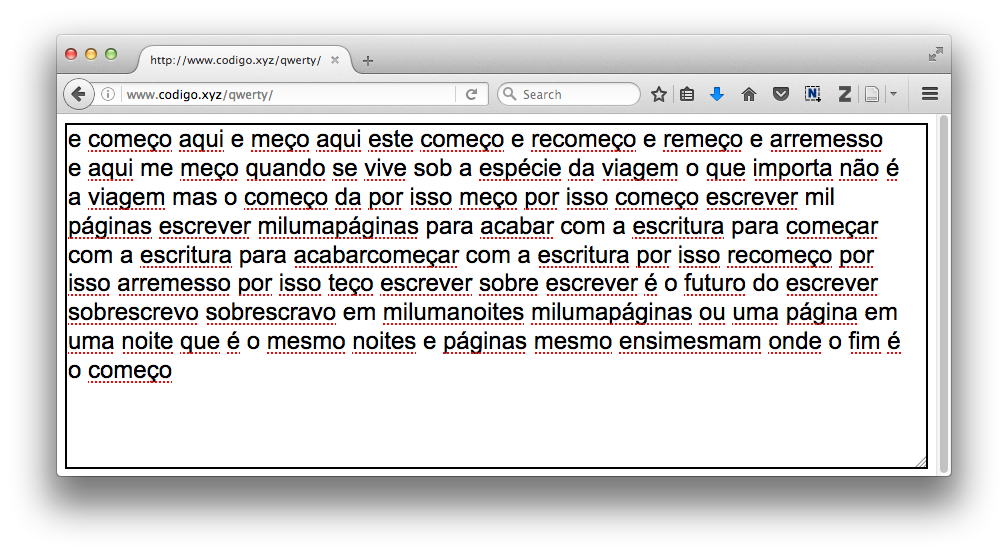
\includegraphics[width=1\linewidth]{pictures/cap3/qwerty.png}
    \end{center}
    \legend{Fonte: Screenshot da autora, Janeiro de 2016}
\end{figure}

Parti do poema Galáxias porque ele é sobretudo extremamente sonoro. O livro acompanha um CD com as leituras de Haroldo de alguns fragmentos do seu texto, e foi de onde extraí os samples usados, buscando uma atomização do discurso, em uma relação com a própria estrutura do poema, que como apontou o poeta Augusto de Campos em conversa com a autora, poderia ter tido sua primeira edição publicada em folhas soltas para ser recombinado, ideia que foi posteriormente abandonada.

Partimos de um processo de escuta buscando encontrar os sons correspondentes a cada letra em nas leituras do poeta e fizemos um mapa onde cada letra digitada do teclado corresponde a um fonema relacionado, criando um \emph{sampler} de 26 sons, que são disparados ao digitar.

A interface desenvolvida foi a mais enxuta possível (figura \ref{qwerty}), pensando em um minimalismo radical que se relaciona com a estética da poesia concreta, e também em uma idéia de brutalismo digital que defendemos no nosso trabalho.

\subsection{Protesta Fora Temer}
Durante o mês de outubro de 2016, surgiu uma discussão na lista de emails da rede Sonora\footnote{A rede sonora (\url{www.sonora.me}) é uma rede organizada para discutir assuntos relacionados a discussões de músicas e feminismos. A rede possui uma lista de discussão por e-mails e um grupo que se reúne presencialmente em São Paulo para propor atividades mais constantes.} sobre a possibilidade de se posicionar contra o impeachment da presidenta Dilma Rousseff. Após uma breve discussão, verificou-se a dificuldade de elaborar um texto que fosse consenso entre as pessoas da rede, devido à ausência de um debate qualificado sobre o assunto e a divergência de opiniões políticas. 
Surgiu então a proposta de organizar um protesto sonoro, e foi lançado um pedido na lista, pela compositora Valéria Bonafé, para quem quisesse participar, que enviasse algum sample em mp3: 
\begin{citacao}

Conversei com algumas membras aqui da Sonora e propus que a gente organizasse um protesto-sonoro-fora-temer. Nossa ideia é montar um protesto sonoro colaborativo e interativo a partir de samples de áudio. O convite está aberto a todo mundo aqui da lista! Quem quiser participar basta enviar um (ou mais!) sample(s) de áudio. As indicações técnicas são apenas duas: que seja curto (questão de alguns segundos) e que esteja em MP3. A ideia é fazer algo leve (no sentido técnico) para não sobrecarregar o sistema de interação que vamos usar para articular esse banco de samples. Como relação ao conteúdo, a única coisa que combinamos é que o mot é “fora temer”. Mas também não precisa ser literal! Não é que precisa gravar apenas falando “fora temer”. Pode ser! Mas pode ser também algo em torno disso. Enfim, temos um tema. Mas cada um pode pensar algo a partir disso. O uso da criatividade, da imaginação, da exploração, da experimentação, da espontaneidade e tudo mais está em aberto! Assim como a “forma”. Pode ser uma gravação nua e crua, pode ser processada, por ser um recorte de algo etc. Enfim, a única diretriz de conteúdo é “fora temer” e a única diretriz técnica é “um sample curto e leve”.
\end{citacao}
Várias pessoas da lista mandaram contribuições e a partir do material enviado. Propus que fizéssemos, ao invés de uma faixa estática, um protesto sonoro interativo. Selecionei 25 samples de áudio e criei uma página HTML onde o movimento do mouse vai soltando aleatoriamente os samples cada vez que passa por cima de uma das palavras no site\footnote{O site está disponível no endereço \url{http://www.sonora.me/protesta/foratemer/}}. O resultado pode ser uma massa de vozes -- a maioria femininas -- ou um coro protestante, dependendo da velocidade que o internauta percorre a página (figura \ref{protesta}). 

\begin{figure}
    \caption{\label{protesta}Protesta Sonora. }
    \begin{center}
    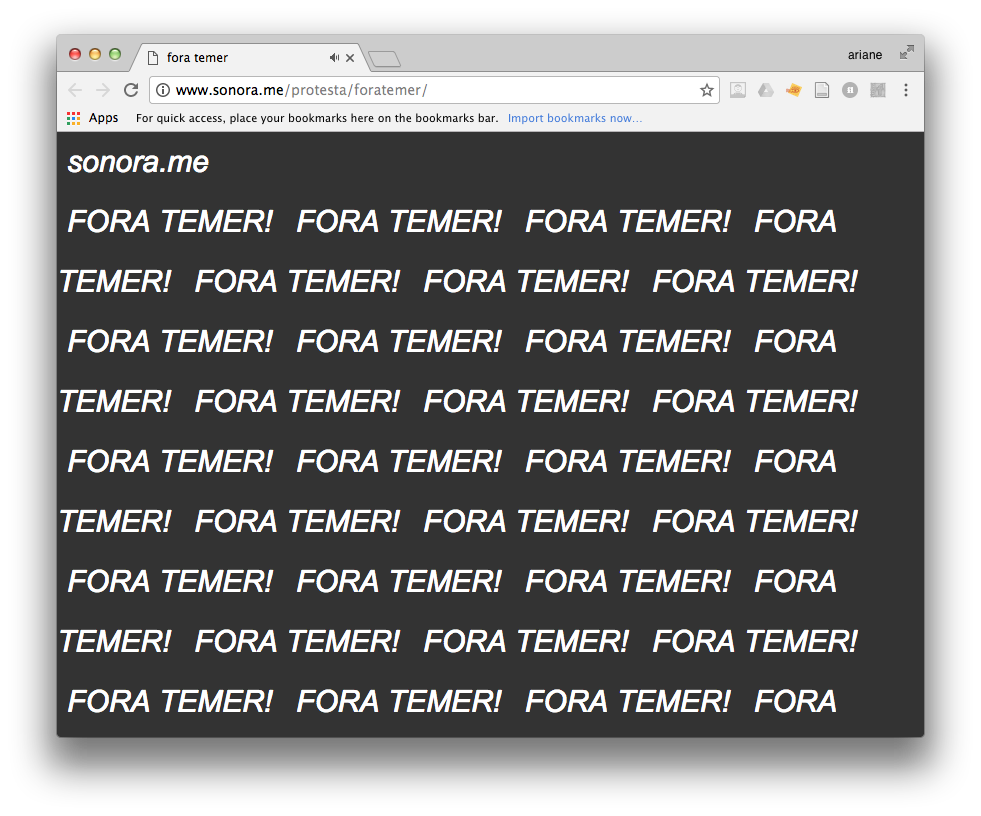
\includegraphics[width=1\linewidth]{pictures/cap3/protesta}
    \end{center}
    \legend{Fonte: Screenshot da autora dia 5 de janeiro de 2016}
\end{figure}



\section{Banda Aberta}

O projeto Banda Aberta começou a ser desenvolvido como parte da proposta do NuSom para o Festival Bigorna na Praça, organizado pelo Estúdio Fita Crepe na praça José Molina. A ideia inicial era conectar os dispositivos pessoais das pessoas pela internet, de modo a potencializar os amplificadores individuais dos celulares e pensar em uma proposta de performance participativa que envolvesse a audiência. Foi o primeiro projeto realizado em parceria com outro programador, o engenheiro de computação Fábio Goródscy, que estava realizando mestrado na Computação musical no IME e o primeiro grande projeto desenvolvido no âmbito desta pesquisa. A parceria com um cientista da computação permitiu que desenvolvêssemos uma estrutura mais complexa do que a dos primeiros experimentos, que ainda eram baseados principalmente em HTML5, e partir para a exploração de recursos mais complexos da Web Audio API \footnote{\cite{Adenot2015}}.

\begin{figure}
    \caption{\label{bandaabertamob}Banda aberta, imagem conceito para a proposta de intervenção pública.}
    \begin{center}
    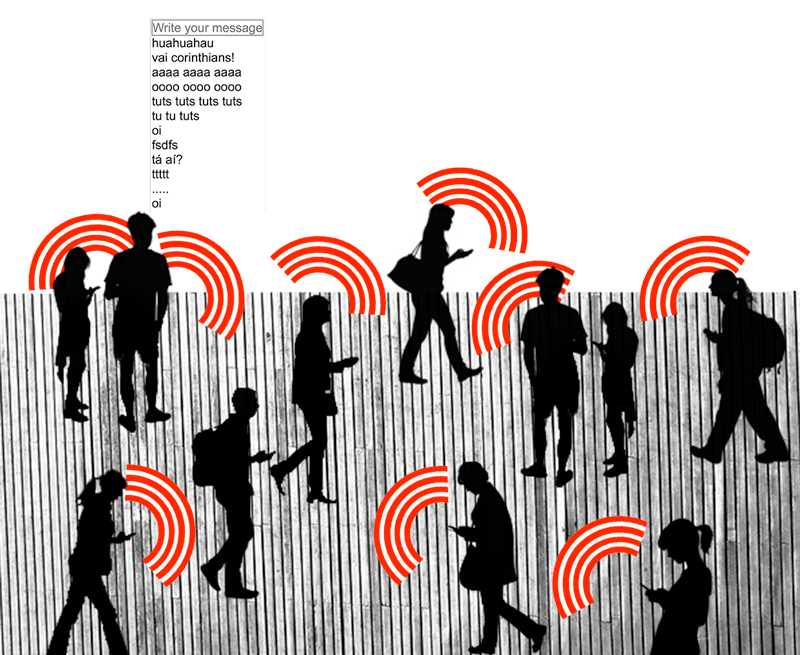
\includegraphics[width=1\linewidth]{pictures/banda_aberta_mob_crowd.png}
    \end{center}
    \legend{Fonte: desenho da autora}
\end{figure}

O principal objetivo desta performance era o dar voz ao coletivo, liberdade de fala, criando também possibilidades de comunicação musical sem significado. Visamos permitir que pessoas em um espaço público venham a interagir em um contexto musical, fazendo um espetáculo produzido por elas mesmas, sem necessidade de nenhum conhecimento musical, utilizando seus próprios celulares via wifi, através de um sistema \emph{open-source} de chat sonoro. A figura \ref{bandaabertamob} apresenta uma imagem conceitual da proposta de performance em um ambiente aberto. 

Performance com participação da audiência mediada por tecnologia é um tópico emergente no campo da tecnologia musical \footnote{\cite{wu2017open}} e na esfera da arte contemporânea. Em contraste com performances tradicionais, onde há uma divisão estrita entre audiência e performer, as performances participativas tendem a diluir os limites entre eles\footnote{\cite{kattwinkel2003audience}}. 

\subsection{Trabalhos relacionados}

Na tradição artística brasileira, esse assunto tem sido explorado desde os anos 60, principalmente no trabalho artístico de neoconcretos como Hélio Oiticica e Lygia Clark. Os parangolés de Oiticica, desenvolvidos a partir de um trabalho do artista com a comunidade da favela da Mangueira no final dos anos 60 eram peças vestíveis, cujo sentido se dava na dança e na manipulação das formas pela comunidade, assim como os Bichos, de Lygia Clark, que são esculturas articuladas que podem ser manipuladas e re-compostas pelo público\footnote{\cite{Braga2008}}. Oiticica incorpora na sua obra uma ``vivência total do expectador'', que ele chama de ``participador''\footnote{\cite{Oiticica1986}}.

\begin{figure}
    \caption{\label{parangole}Participadores vestindo parangolés de Hélio Oiticica}
    \begin{center}
        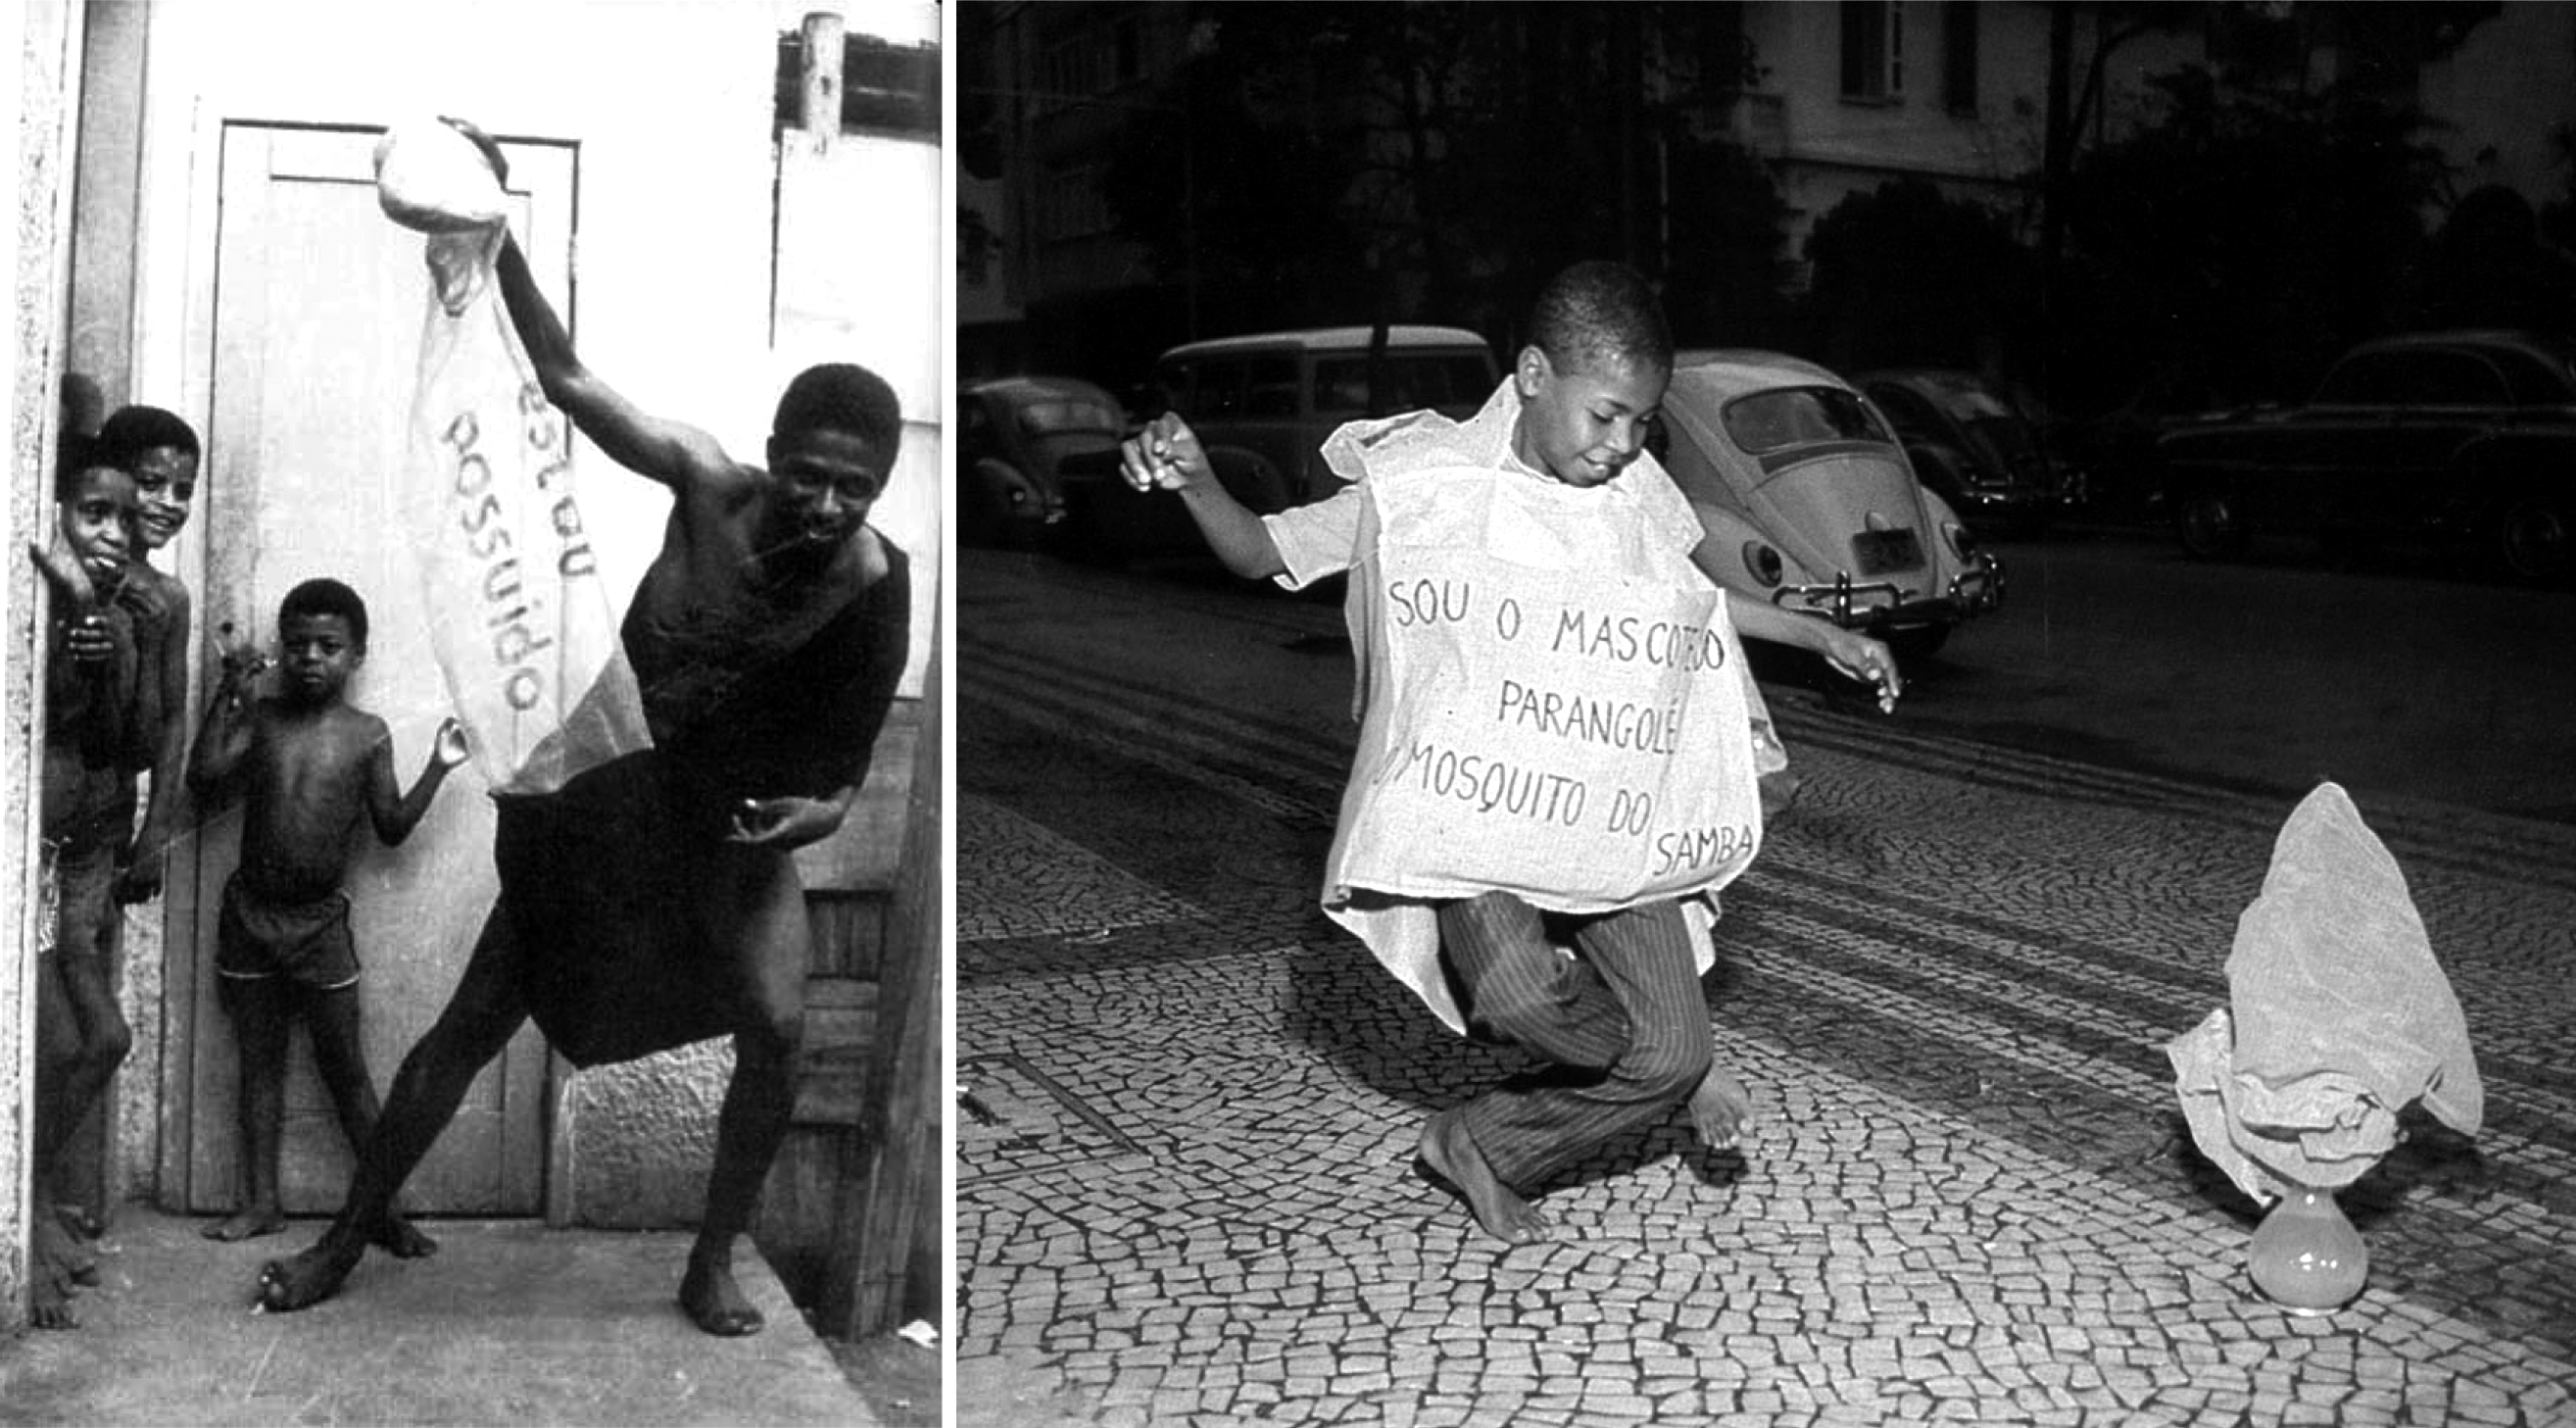
\includegraphics[width=1\linewidth]{pictures/cap3/parangole}
    \end{center}
    \legend{Fonte: JACQUES, 2001 e Catálogo da Retrospectiva de Hélio Oiticica, 1986 in \cite{Girnos2006}.}
\end{figure}

Atualmente, o desenvolvimento da tecnologia trouxe novos recursos para facilitar e encorajar processos participativos em performances e instalações como: dispositivos computacionais portáteis como Arduino\footnote{Plataforma eletrôncia em código aberto Arduino: \url{https://www.arduino.cc/}} ou Bela\footnote{Plataforma para processamento de áudio de baixa latência Bela: \url{http://bela.io/}}; smartphones; sensores e novas linguagens versáteis de alto nível como Python e JavaScript, que também ajudaram a criar as bases para o campo de pesquisa da ``computação ubíqua''. Diversos projetos utilizam tecnologias deste tipo para o emprego criativo da participação da audiência em performances ao vivo.

O projeto massMobile (\citeyear{Weitzner2012}), usa uma interface web controlada por um servidor que se conecta a um patch em Max/MSP que por sua vez controla os clientes utilizados pelos participantes nas performances. Funciona como um \emph{framework} que permitiu uma série de demonstrações diferentes no Georgia Tech institute. Em uma delas participantes podiam tocar através de uma matriz de tons, que é um ``paradigma clássico'' das interfaces musicais\footnote{\cite{Weitzner2012}}. Já na peça ``Saxophone Etudes'', de Jason Freeman, o \emph{framework} foi utilizado como um sistema de votação em tempo real para escolher partes da partitura que eram tocadas pela performer. A audiência também podia escolher o quão rápido ou devagar eles queriam que a música fosse tocada\footnote{\cite{Freeman}}.  


 %como os projetos massMobile , Mood Conductor \footnote{\cite{Fazekas:2014}}, Open Symphony \footnote{\cite{wu2017open}}, Crowd in Cloud \footnote{\cite{Lee2016}} e TweetDreams \footnote{\cite{Dahl2011}}. Em condições ideais, os participante são capazes de interagir durante as performances interferindo na narrativa de modo sensível. 

Receber \emph{feedback} da audiência para performances de improvisação ao vivo é um dos modos como as tecnologias móveis têm sido empregadas em performances participativas atualmente. O ``Mood Conductor'', e o ``Open Symphony'' são dois projetos desenvolvidos na QMUL nesse sentido. O ``Mood Conductor'' (Figura \ref{moodconductor}) funciona por meio de um aplicativo de celular, onde a audiência pode escolher contextos emocionais para que músicos improvisem em tempo real durante performances\footnote{\cite{Fazekas:2014}}. Já no Open Symphony \footnote{\cite{wu2017open}}, a audiência interage através de um site, escolhendo morfologias sonoras para os músicos explorarem. 

\begin{figure}
    \caption{\label{moodconductor}Mood Conductor sendo utilizado em performances na Inglaterra}
    \begin{center}
        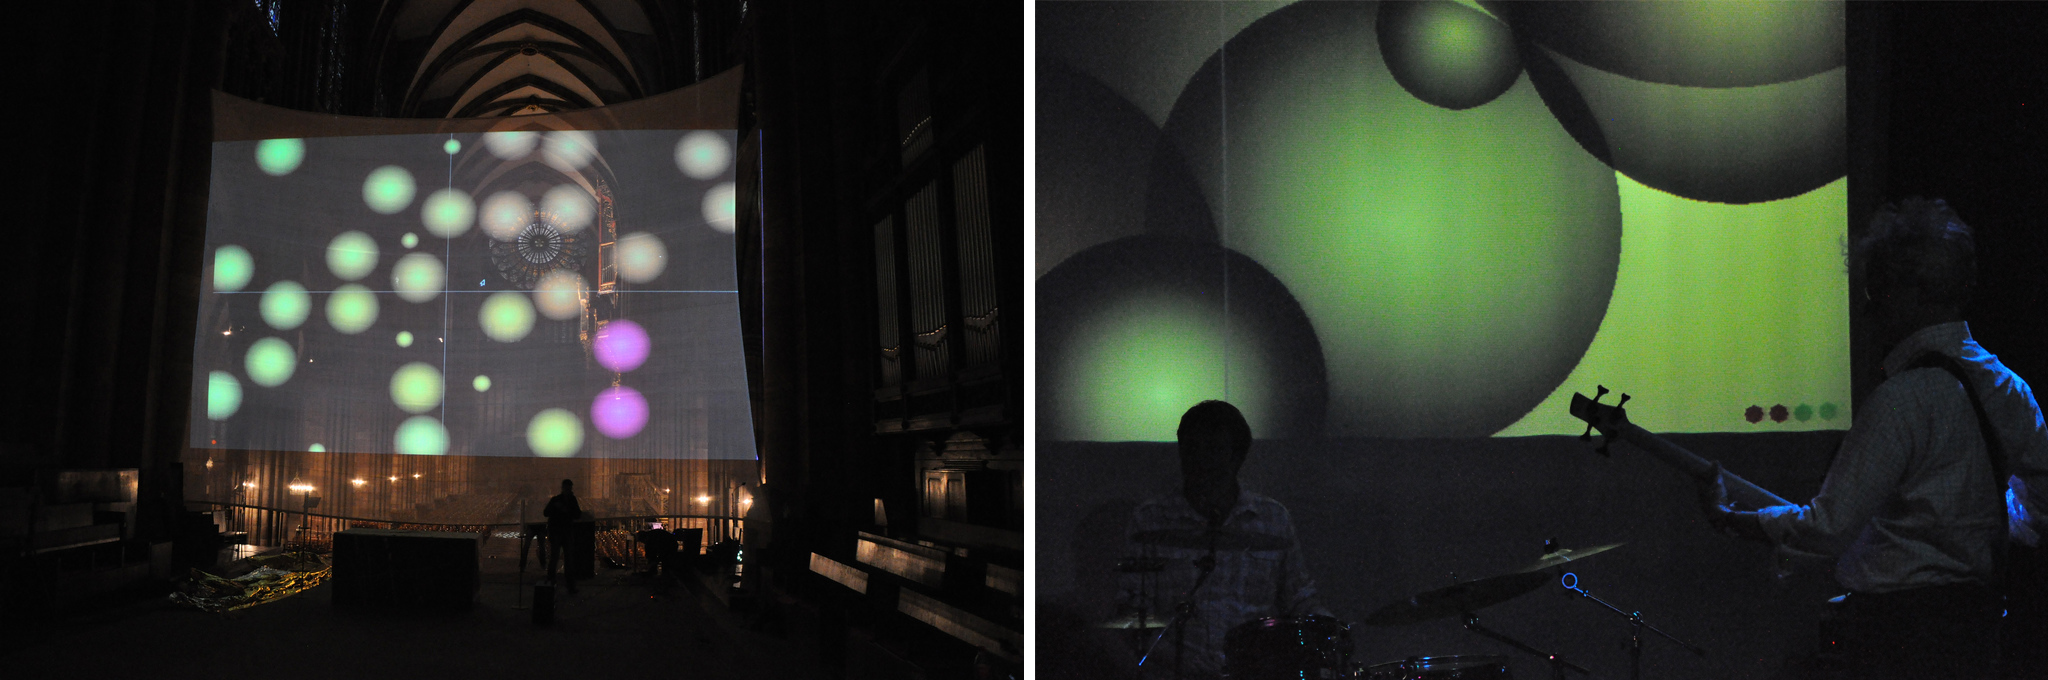
\includegraphics[width=1\linewidth]{pictures/cap3/moodconductor}
    \end{center}
    \legend{Fotos: Matheiu Barthet.}
\end{figure}

\begin{figure}
    \caption{\label{moodconductor}Open Symphony}
    \begin{center}
        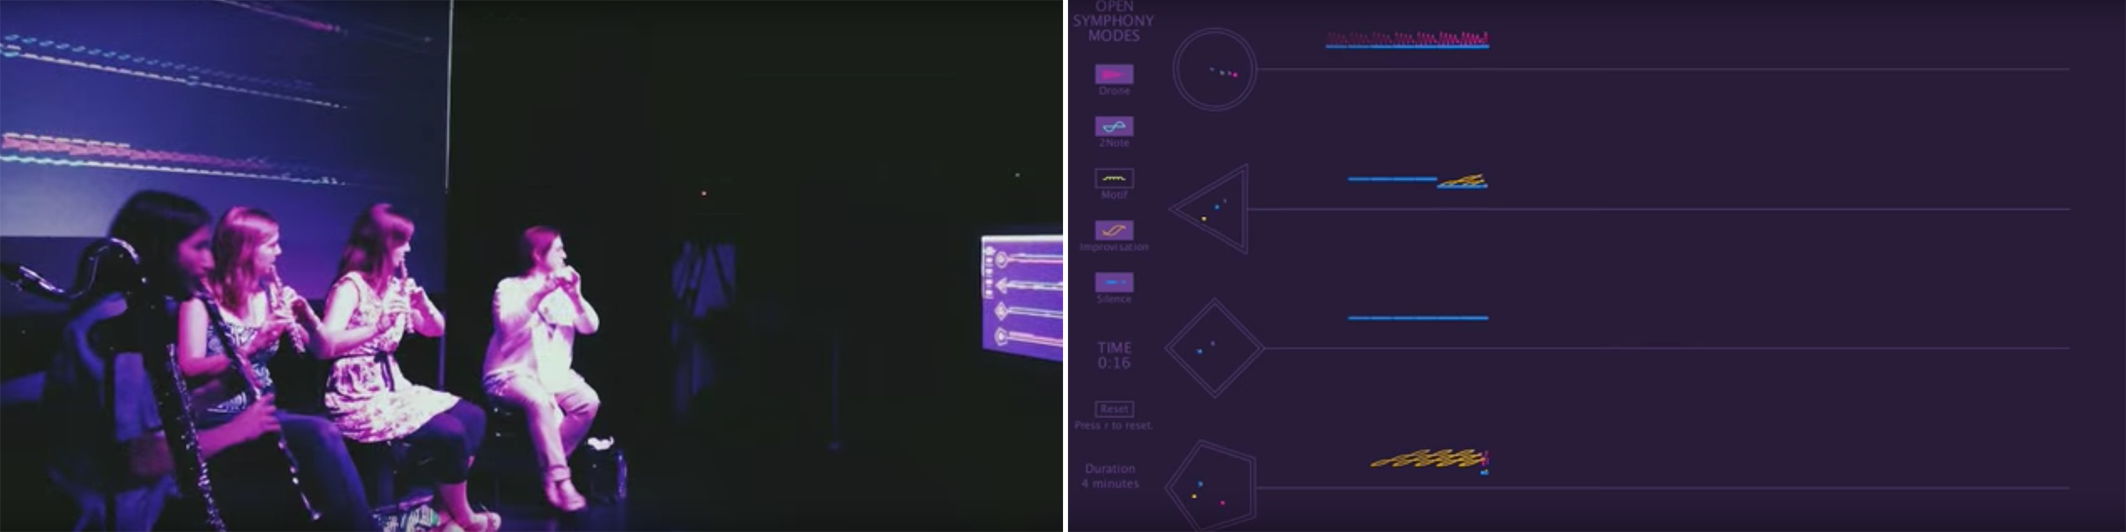
\includegraphics[width=1\linewidth]{pictures/cap3/opensymphony}
    \end{center}
    \legend{Fonte: \url{https://youtu.be/Syxfznk36Nc
}.}
\end{figure}

Em outros, a participação da audiência acontece também no processo de tocar, como na peça Crowd in c[loud] de Sang Won Lee\footnote{\cite{Lee2016}}, que é inspirada em aplicativos de relacionamento \emph{online}. Na peça, cada membro da audiência compõe um trecho curto de música em uma escala de Dó maior. Em seguida, pode navegar pelas peças compostas pelos demais participantes e decidir se gosta ou não gosta dos trechos que os outros participantes compuseram, podendo dar \emph{match} caso ambos gostem um do som do outro (Figura \ref{crowdincloud}). O performer, por sua vez, acompanha as interações dos usuários e toca os trechos mais populares entre audiência em tempo real.

\begin{figure}
    \caption{\label{crowdincloud}Interface da audiência na peça Crowd in c[loud]}
    \begin{center}
        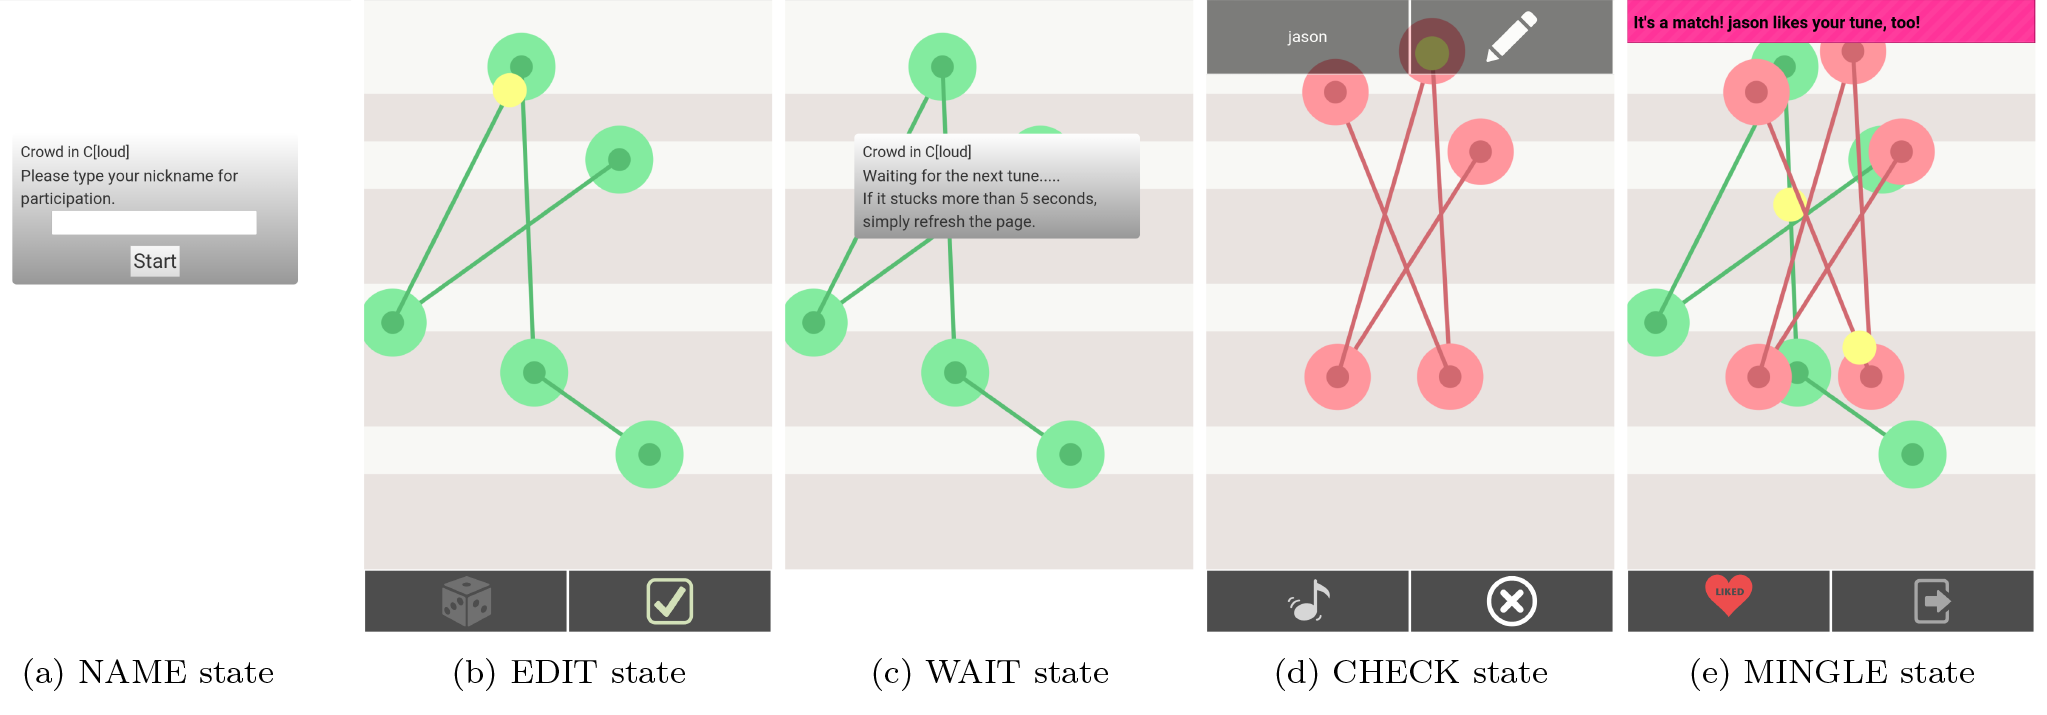
\includegraphics[width=1\linewidth]{pictures/cap3/crowdincloud}
    \end{center}
    \legend{Fonte: \url{https://youtu.be/Syxfznk36Nc
}.}
\end{figure}

``TweetDreams'', de Luke Dahl, Jorge Herrera e Carr Wilkerson\footnote{\cite{Dahl2011}}, calcula melodias a partir de informações de postagens no Twitter recebidas em tempo real\footnote{Postagens são recuperadas usando Python e as melodias através do framework Chuck. Um vídeo da performance está disponível em: \url{https://ccrma.stanford.edu/groups/tweetdreams/}}. Durante performance, a audiência é encorajada a fazer postagens no Twitter, que são recuperadas e sonificadas pelos performers. 


\begin{figure}
    \caption{\label{crowdincloud}Tweetdreams, de Luke Dahl, Jorge Herrera e Carr Wilkerson}
    \begin{center}
        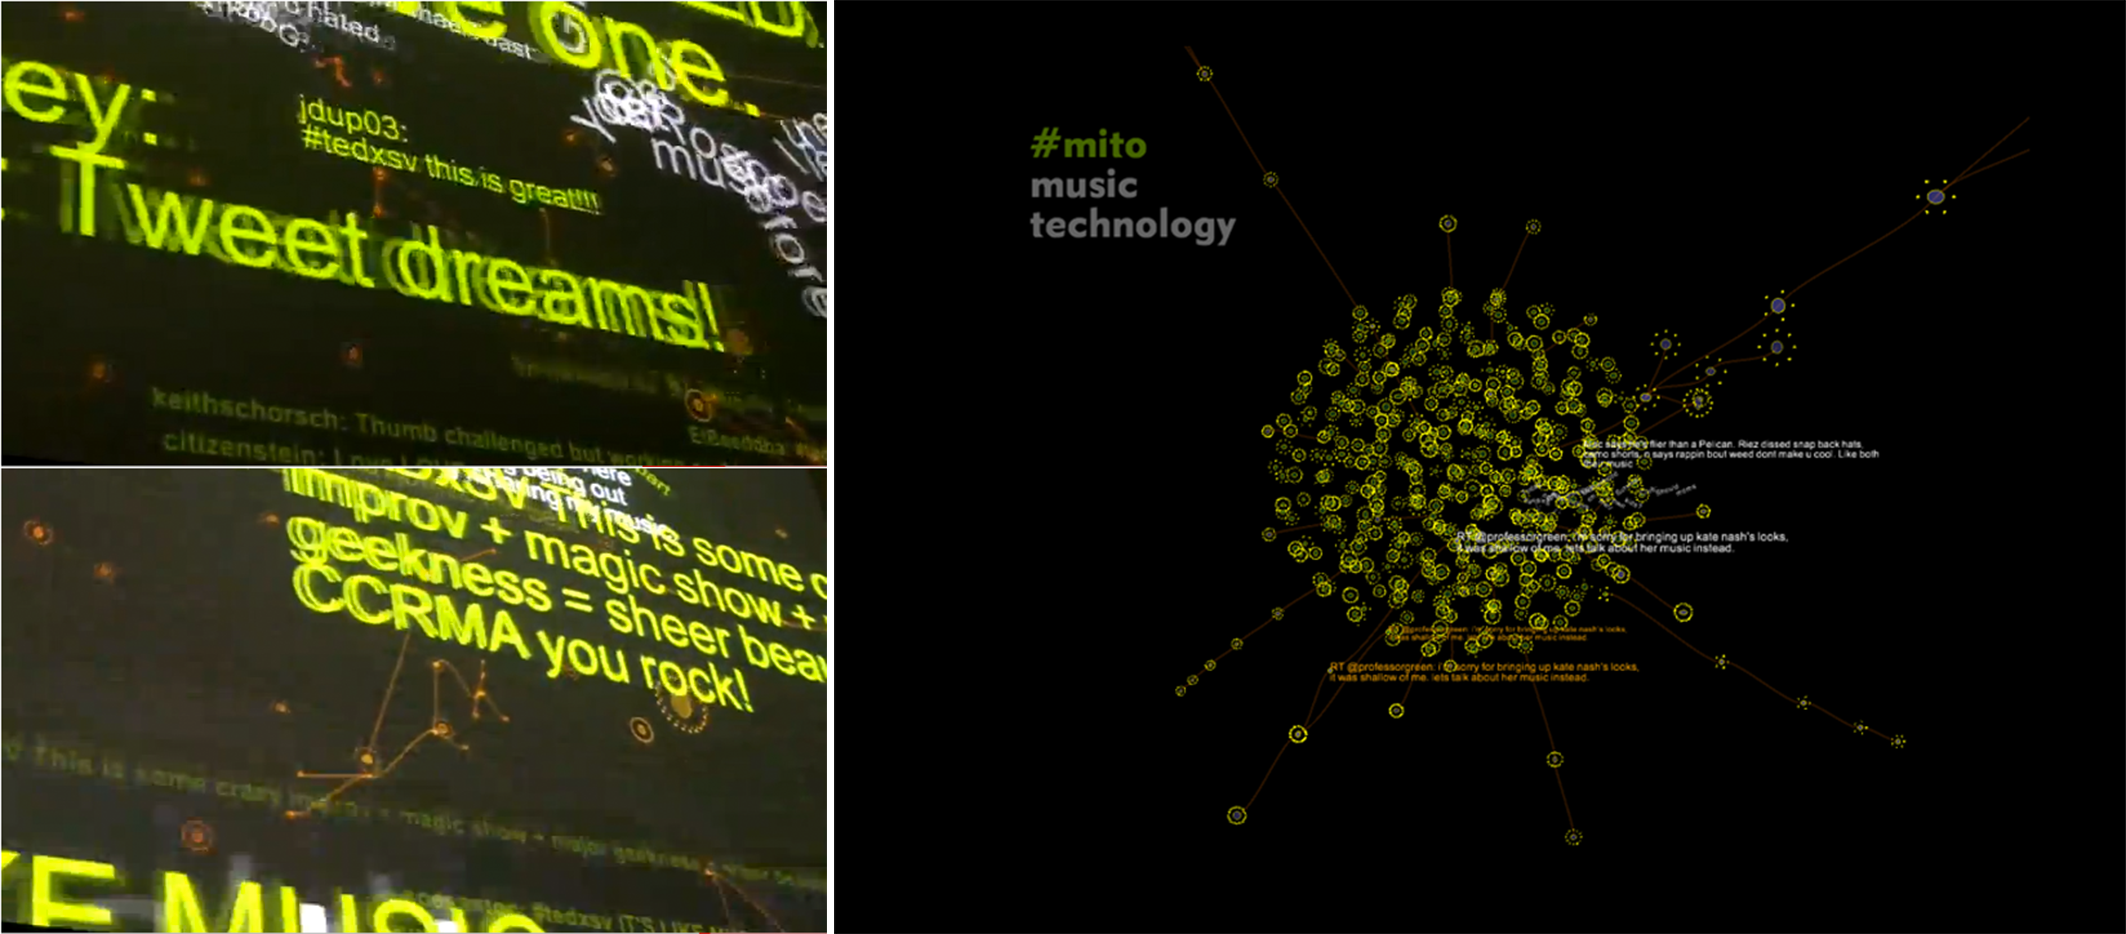
\includegraphics[width=1\linewidth]{pictures/cap3/tweetdreams}
    \end{center}
    \legend{Fonte: \url{https://ccrma.stanford.edu/groups/tweetdreams/}.}
\end{figure}


%Concert for Smartphones Andrey Bundin
%The performance involves audience participation with their mobile devices. Connected to a wireless network and organized into one polyphonic multichannel synthesizer, those devices reproduce different noises, samples, and synthesized sounds from random locations in the hall. In addition, loudspeakers complement the phone choir to add dynamic climaxes and low-frequency effects. The name of the performance refers to academic music traditions. The author emphasizes the similarity in musical nature of the Concert for Smartphones and any classical concert for soloist and orchestra. The performance is an experiment in exploring possible ways of using an audience’s mobile devices as a medium for sound diffusion in the context of a traditionally composed electroacoustic musical piece.

O projeto Banda Aberta é uma tentativa de explorar esse tema, usando a música como ponto de partida, pela função social que ela tem de comunhão e comunicação \footnote{\cite{Koelsch:2014}}. A idéia era de propor uma obra ``aberta'', como defendida por Umberto Eco \footnote{\cite{Eco1991}}, que, de acordo com Robey \footnote{Robey in \cite{Eco1991}}, requer do público um grau muito maior de envolvimento pessoal e colaboração do que qualquer obra de arte tradicional do passado. Segundo Eco, em uma obra aberta, ``é decisão do artista de deixar com que parte da organização de seus constituintes seja relegada ao público ou ao acaso, dando a elas assim não uma ordenação definitiva, mas uma multiplicidade de ordens possíveis'' \footnote{\cite{Eco1991}}.

Com o projeto Banda Aberta, nós queríamos criar um sistema que pudesse ser facilmente utilizado como um instrumento musical pelos participantes, independente de qualquer conhecimento musical a priori. O projeto de ambientes colaborativos para produção musical pode ser desafiador, no sentido de que a audiência não necessariamente compartilha de domínio de técnicas e processos musicais. Blaine (\citeyear{Blaine2003}) aponta ``severas limitações impostas'' aos designers que desejem criar interfaces que permitam a participação de noviços em experiências sonoras coletivas: 

\begin{citacao}
Se uma pessoa tocando se sentir excluída devido à percepção de falta de habilidade, não vai ter uma experiência positiva. Esse é frequentemente o caso de instrumentos musicais tradicionais, que exigem uma prática significativa para se tocar bem. Essencialmente, acessibilidade de baixo nível é necessária para que as pessoas interajam com os instrumentos e entre-si.\footnote{\cite{Blaine2003}, tradução nossa}
%If a player feels excluded due to a perceived lack of skills, she does not have a positive experience. This is often the case with traditional musical instruments that require significant practice to play well. Essentially, low-level accessibility is necessary for people to participate and interact with the instruments and each other. Finally, most of the interfaces we consider are intended for public exhibition, where people casually “walk-up and play.” This restricts the amount of time that a designer can expect someone to spend learning an interface and necessitates highly constrained interfaces that are conducive to musically accessible flow-through experiences.

\end{citacao}

Além disso, aponta ela, esse tipo de experiência conta em geral como público pessoas passantes que estão presentes para tocar casualmente, o que exige que se pense em um tempo muito reduzido de aprendizado antes de tocar o intrumento. Existem vários tipos de interface para participação musical que partem de gestos de toque, simulando um processo de interação similar ao dos instrumentos tradicionais, como por exemplo a performance ``88 Fingers'' de Norbert Schnell e Benjamin Matuszewki \footnote{\cite{Schnell2017}}, onde cada participante pode controlar através do celular uma das teclas de um piano MIDI, ou ``Hyperconnected Action Painting", de Anna Xambó e Gerard Roma \footnote{\cite{Xambo2017}}, onde a audiência usa gestos com o celular para disparar sons pré definidos. 

Apesar de ambas serem divertidas como experiências participativas, o resultado sonoro nesses dois casos, na minha impressão como participante, foi de uma massa de sons desordenada e fora de ritmo. Isso aconteceu em parte pela falta de prática em processos musicais coletivos por parte da audiência, que não necessariamente domina o gestual musical. Pensando nessa questão, queríamos propor uma ferramenta que pudesse ser acessada por qualquer usuário, independente de qualquer formação ou treinamento em práticas musicais, e para isso, procuramos partir de tecnologias que as pessoas já usam com mais desenvoltura.

\subsection{Desenvolvimento do Projeto}
Como já apontava McLuhan\footnote{\cite{mcluhan1968comunicaccoes}}, o alfabeto fonético é uma tecnologia fundamental para o desenvolvimento da cultura ocidental. Ele é fácil de se aprender e ajustável a várias linguagens, sendo assim, a base de toda cultura literata. Neste trabalho, nós fazemos uso do alfabeto como tecnologia para produzir música experimental. Texto e mensagens instantâneas se tornaram a principal forma de comunicação nos celulares hoje em dia, seja em comunicações síncronas ou assíncronas \footnote{\cite{Madell:2007}}, e por isso, decidimos experimentar com  o texto através de mensagens como forma de interação musical nesta primeira proposta. Muitos tipos de interfaces para produção musical usam o texto como forma de \emph{input}, como nos processos de \emph{live coding} \footnote{\cite{Collins2003}}, em processos participativos que usam \emph{feedback} verbal da audiência \footnote{\cite{noauthor_transglasphone_nodate}}, em composições algorítmicas geradas por dados textuais ou sistemas que usam o teclado como controlador musical \footnote{\cite{Fiebrink2007}}. Neste projeto, nós procuramos criar um sistema que funcionasse para a produção musical de uma maneira análoga ao alfabeto e sua relação com a linguagem oral.

A comunicação \emph{online} por texto se aproxima muito da comunicação oral, pela facilidade de escrita, e pela velocidade quase instantânea,\footnote{\cite[33]{Levinson2001}} Como aponta McLuhan, o conteúdo de um meio sempre agrega um meio anterior. O discurso, que é o meio mais antigo, está contido em quase todos meios subsequentes, como o livro, o telégrafo, o cinema e a televisão, e, é claro, a internet \footnote{\cite[42]{Levinson2001}}. 

McLuhan aponta que o espaço visual surge quando as consoantes foram criadas, ``como uma abstração sem significado", permitindo a análise das unidades silábicas em cada um de seus componentes. A consoante é para ele um não-som, algo que necessariamente ``soa junto". \footnote{\cite[13-14]{mcluhan1968comunicaccoes}} A base do discurso, segundo ele é o fonema, a unidade mínima do som, que seria a unidade mínima do som. Na música, no entanto, Tenney (\citeyear{Tenney1988}) propõe em ``Meta-Hodos and Meta Hodos" o conceito de ``clang", que seria uma unidade \emph{gestalt} mínima reconhecível \footnote{\cite[23]{Tenney1988}}. 

Neste projeto, ao buscarmos o som das consoantes de um modo isolado, criamos uma desconstrução do discurso e procuramos reforçar esse caráter atomizante da linguagem escrita através de um duplo processo de conversão: discurso convertido em texto e posteriormente convertido em música.

A digitação é um processo muito mais simples para a maioria dos usuários de computadores e dispositivos digitais, em relação à operação de interfaces musicais, assim como a digitação na máquina de escrever era mais acessível para o homem comum do que o tocar de instrumentos analógicos. \footnote{\cite[172]{Levinson2001}}. Nossa ideia foi utilizar o \emph{input} de texto como forma de interação musical. 

Num projeto realizado previamente, o QWERTY, já tinha começado a explorar a digitação como forma de entrada, mapeando cada letra do teclado para um sample, que eram disparados de acordo com a digitação. Nós percebemos que isto exige do performer uma certa habilidade de controle do gesto, para que os sons saiam em ritmo. Além disso, como as interfaces dos \emph{smartphones} não facilitam a digitação, queríamos pensar um sistema que não dependesse de agilidade para funcionar. Para encorajar a participação, nós projetamos um sistema que funcionava a partir de simples mensagens de texto.

No nosso projeto, utilizamos as frases como disparadores para uma sequência de samples, que são já compostos com durações fixas, num processo análogo ao de composição de frases musicais. Ao colocar um mecanismo de \emph{chat}, as pessoas podem acessar o instrumento simultaneamente e participar de um diálogo sonoro. Conforme mais pessoas vão escrevendo simultaneamente, a camada de \emph{samples} se torna mais densa e entrópica.

Diferente de processos de síntese vocal, nosso chat não concatena as sílabas, somente toca os sons pré-determinados em uma sequência, de modo que as palavras não são compreendidas como palavras, mas como frases musicais. Para adicionar um certo grau de controle à performance, utilizamos uma lógica da interface por linha de comando, com de certos comandos especiais desconhecidos pela audiência que podem alterar a dinâmica da peça, ou alternar entre os conjuntos de samples compostos.

O projeto é construído a partir de dois dispositivos, o servidor de mensagens, que é programado em \emph{Ruby} e necessita de instalação em um servidor web, e a interface que faz o processamento das mensagens e é construída em HTML e \emph{JavaScript} e funciona a partir da Web Audio API.    

\begin{figure}
    \caption{\label{bandaabertaserver}Diagrama esquemático dos servidores do projeto Banda Aberta}
    \begin{center}
        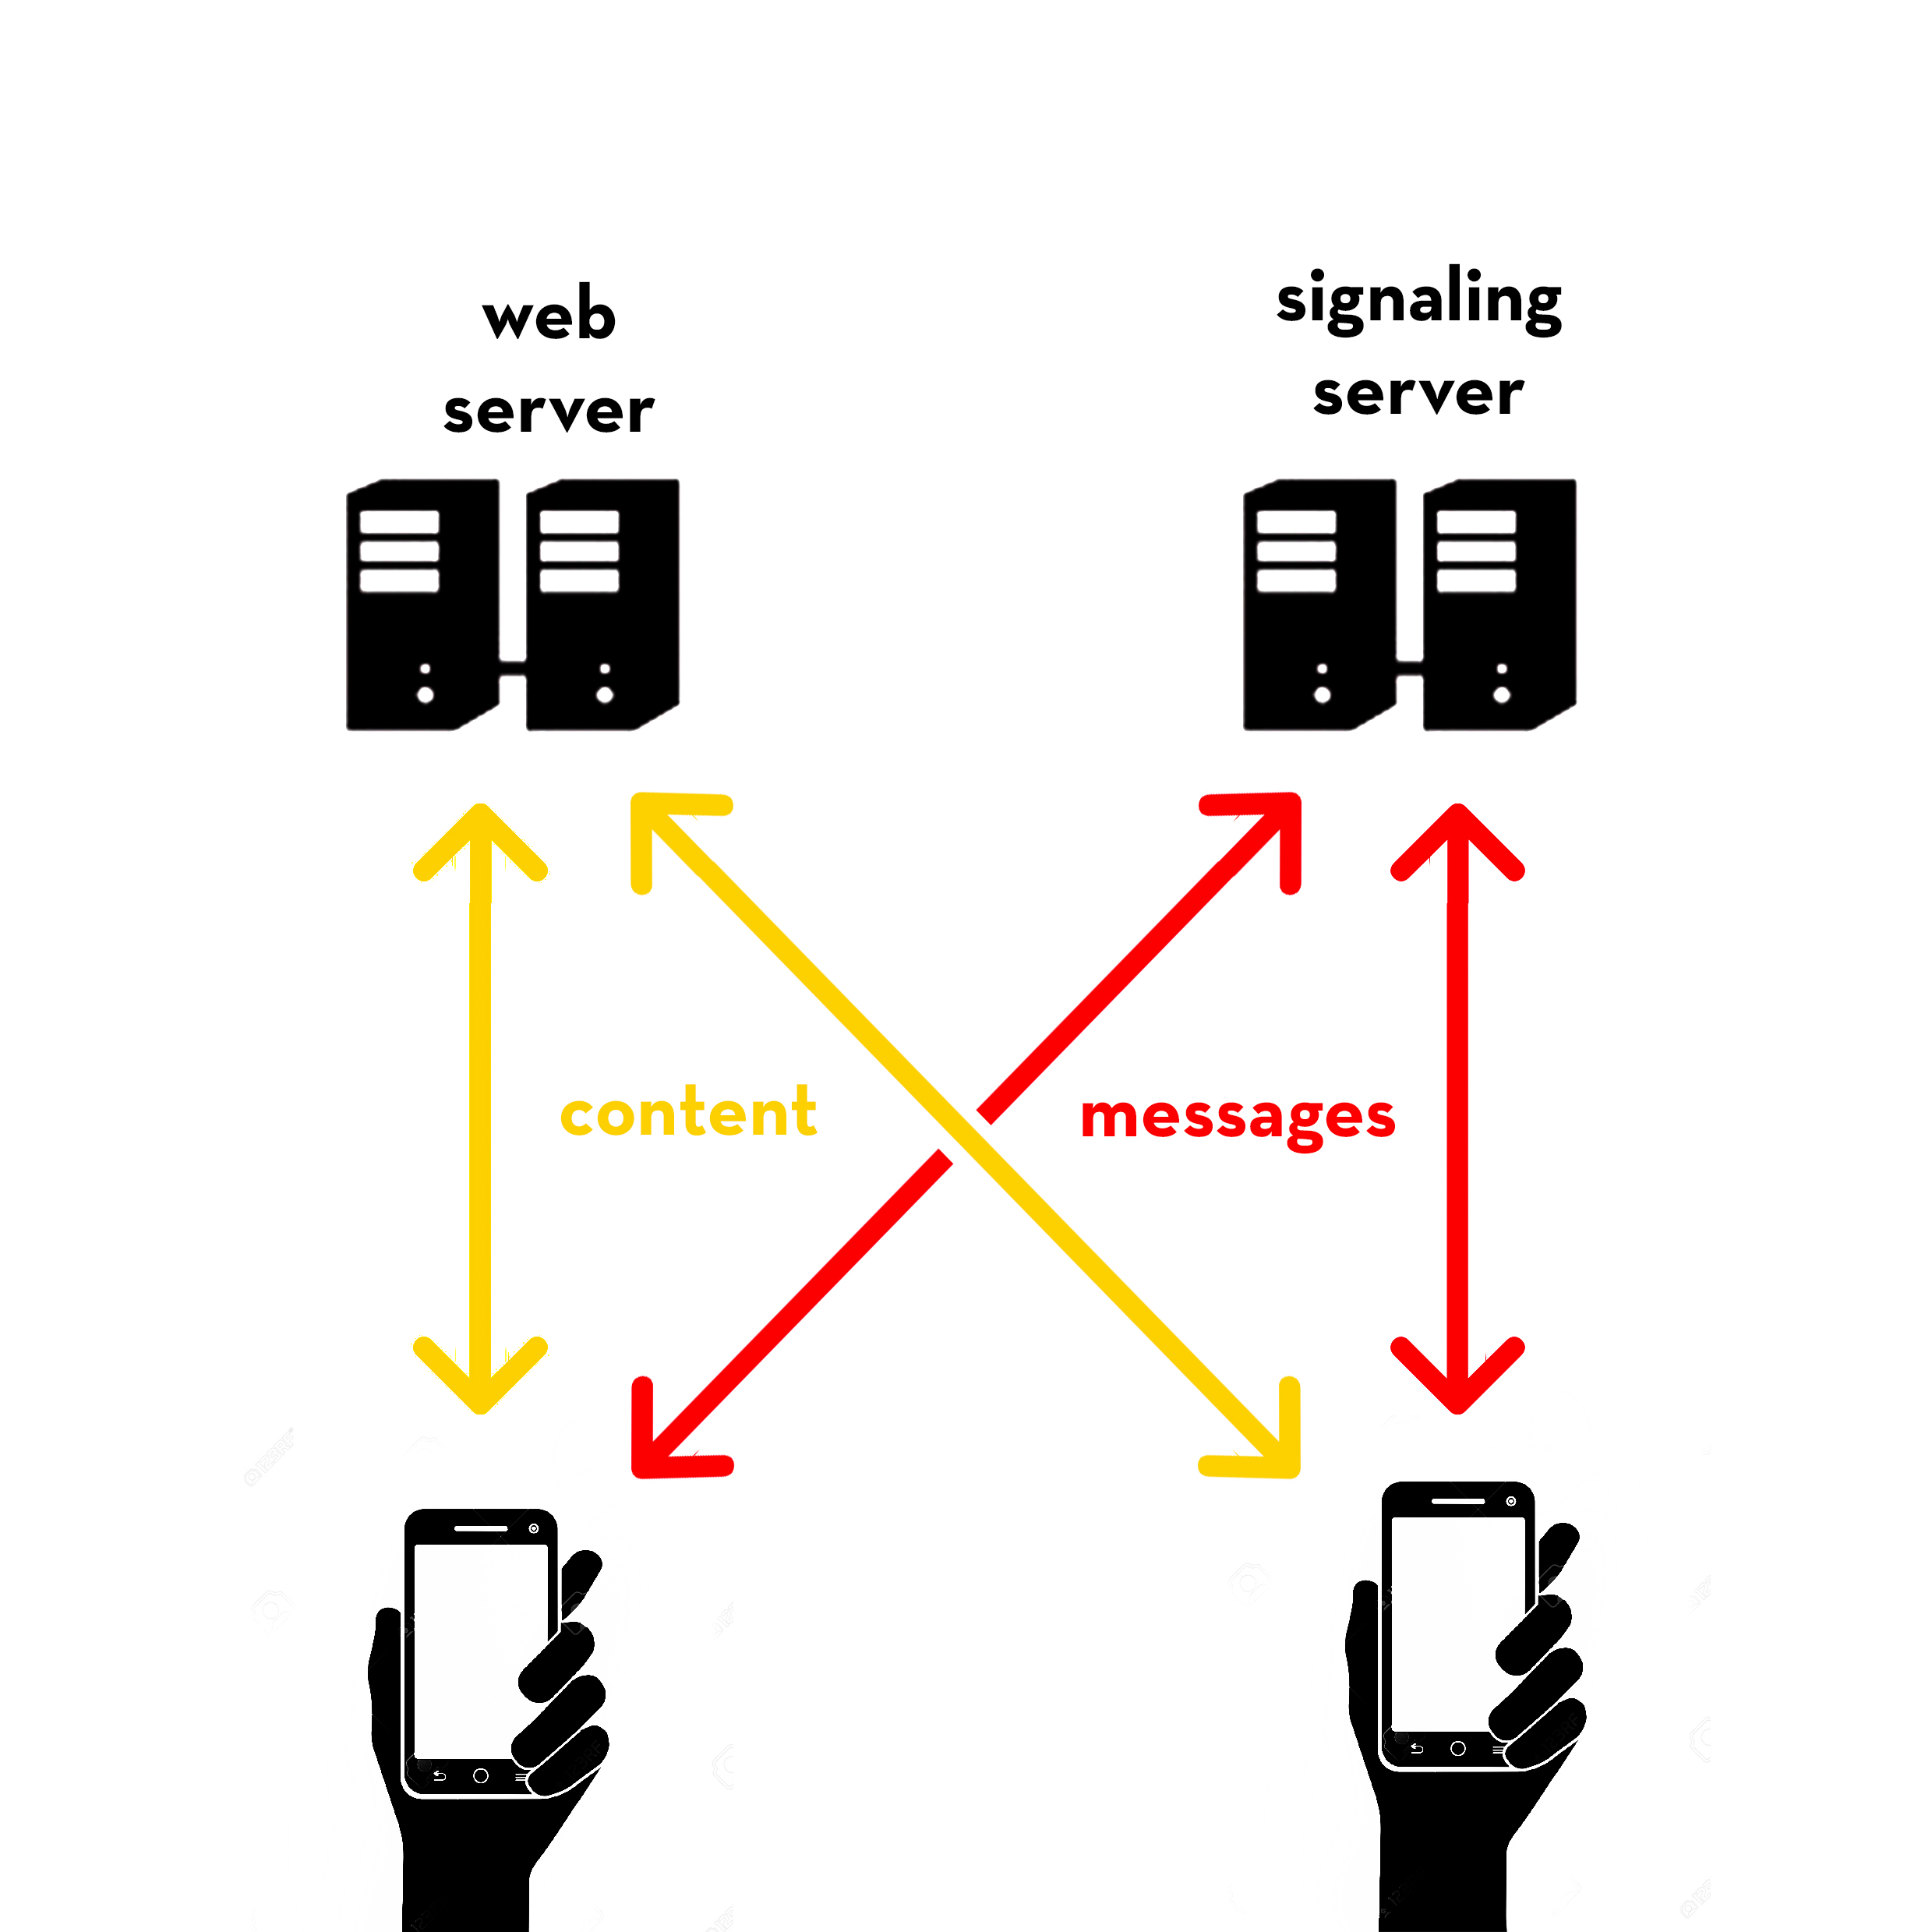
\includegraphics[width=0.5\linewidth]{pictures/server.jpg}
    \end{center}
    \legend{Fonte: desenho da autora}
\end{figure}

Na primeira versão, o processamento de áudio funcionava somente por sampleamento. Os \emph{samples} são numerados de acordo com a tabela de ASCII e um sample foi designado para caractere dela. O sistema converte as letras nos números equivalentes segundo a tabela, e toca o sample respectivo segundo a ordem estabelecida por cada frase enviada. Posteriormente, desenvolvemos também uma segunda versão baseada somente em síntese sonora no navegador.

\subsection{Desenvolvimento do Projeto}
Para o desenvolvimento do projeto Banda Aberta, adotamos ``Lean UX'' como metodologia de design, uma metodologia ágil de desenvolvimento de software que tem sido aplicada em muitos projetos de webdesign \footnote{\cite{leanux}}. Envolve a criação de um protótipo mínimo e viável a partir de um estágio muito inicial do projeto. Este protótipo deve então ser testado em condições reais de uso e melhorias são feitas de modo iterativo, baseando-se em observações e \emph{feedbacks} recolhidos. O projeto foi desenvolvido como software de código aberto e está disponível no Github. \footnote{Os códigos-fonte do projeto estão disponíveis em: \url{https://github.com/fabiogoro/bandaserver}}. A arquitetura do sistema foi descrita com mais detalhes no artigo publicado na conferência Audio Mostly de 2017 ``Open Band: A Platform for Collective Sound Dialogues''\footnote{\cite{Stolfi2017}}.

Nosso primeiro protótipo contava apenas com o conjunto inicial de samples nomeado de ``Galáxias'', e pudemos testá-lo menos de um mês após a proposta inicial em uma reunião do NuSom. Os samples utilizados nessa primeira versão eram os mesmos reunidos para o experimento QWERTY, descrito na seção \ref{sec:QWERTY}. A experiência foi registrada e fizemos uma análise dos comentários dos participantes\footnote{Registro da experiência pode ser visto em: \url{https://www.youtube.com/watch?v=Utc_4mT5b8s}}. Pudemos notar desde o princípio que a performance tinha um certo grau de ludicidade, pelas reações de riso e divertimento dos presentes. 


Neste primeiro teste em público, notamos que haviam alguns problemas com relação à compatibilidade de aparelhos, que foram posteriormente corrigidos. Recebemos também a opinião de alguns usuários que notaram que após alguns minutos a experiência sonora passava a ser um pouco entediante, com a repetição constante dos mesmos sons. Propusemos então a criação de outros bancos de sons, que seriam alternados durante a performance, e que um deles fosse criado colaborativamente por um grupo de estudantes da Universidade Anhembi Morumbi, orientados pelo professor Vítor Kisil,  que também apresentariam uma peça no Festival Bigorna. A partir daí, compusemos os demais pacotes de samples discutidos na seção \ref{sec:trad}



%\begin{figure}
   
       %\includegraphics[width=1\linewidth]{pictures/audiotype_sketch}
 %  \caption{Primeiro teste do projeto Banda Aberta realizado no NuSom.}
  %  \label{fig:testenusom}
 %\end{figure}
Nós queríamos assegurar a acessibilidade da audiência e garantir uma flexibilidade na montagem da performance, garantindo seu funcionamento mesmo em locais sem disponibilidade de acesso à Internet, o que seria o caso do Festival Bigorna. Para isso, utilizamos um roteador wifi para criar uma rede local aberta onde os usuários podiam ter acesso ao sistema em um servidor local (esta prática é frequentemente utilizada como estratégia para permitir a participação da audiência em sistemas de música móvel\footnote{\cite{Lambert:2016}}). Uma questão em performances participativas via celulares é que muitas vezes os usuários podem se distrair usando a internet, por informações vindas de outros aplicativos como de trocas de mensagens ou redes sociais\footnote{\cite{wu2017open}}, isto também é evitado pela rede local, que isola os usuários da internet, deixando os mais focados na performance e na experiência resultante. Durante as performances, os participantes acessaram o sistema através de um endereço IP que direcionava para uma máquina local com o servidor.

Nossa intenção era de que os participantes pudessem interagir com pouca ou nenhuma explicação anterior. No início das apresentações, passávamos somente instruções de qual endereço acessar, e uma vez na página há um campo de entrada de texto com a informação ``envie sua mensagem''. O endereço IP e o nome da rede eram informados também em uma projeção na tela (na maioria das performances). Um site com uma versão online é mantido no ar desde o lançamento do projeto e pode ser acessado no endereço: \url{banda.codigo.xyz}




\subsection{Tradução Inter Semiótica}
\label{sec:trad}

%

Neste projeto, queríamos manter uma relação semântica entre as letras utilizadas nas mensagens e o resultado sonoro gerado. Para isso, buscamos algumas formas de tradução intersemiótica entre os caracteres e os sons, que fosse além dessa analogia com as teclas de piano. A tradução semiótica é um procedimento utilizado para traduzir diferentes códigos, como aponta Plaza: 

\begin{citacao}
Na tradução intersemiótica como transcriação de formas o que se visa é penetrar pelas entranhas dos diferentes signos, buscando iluminar suas relações estruturais, pois são essas relações que mais interessam quando se trata de focalizar os procedimentos que regem a tradução. Traduzir criativamente é, sobretudo, inteligir estruturas que visam à transformação de formas. \footnote{\cite[71]{JulioPlaza1969}}
\end{citacao}

Aplicar um processo de tradução inter-semiótica de texto para som se relaciona com a idéia de áudio semântico \footnote{\cite{Kostek:2010}}, mas não no sentido tradicional, já que o objetivo aqui não foi o de dar sentido semântico aos sons, mas sim o de explorar quais poderiam ser os significados das letras próprias quando transformadas em sons. A abordagem foi de produzir os \emph{samples} de acordo com o conceito de James Tenney \footnote{\cite{Tenney1988}} de ``Clang'', ou ``gestalt aural", que é similar também ao conceito de objeto celular de Pierre Schaeffer: objetos sonoros breves ou redundantes \footnote{\cite{Chion1983}}. A ideia foi pensar em átomos que pudessem ser recombinados livremente na medida em que as mensagens fossem escritas. Este procedimento aumenta as possibilidades paratáticas do sistema ao permitir re-combinações para além das possibilitadas pela linguagem escrita.


O uso do teclado do computador como \emph{input} para produzir sons em instrumentos musicais digitais pode ser relacionado muitas vezes com o teclado de piano, mas de uma forma limitada, já que a sensibilidade das teclas do teclado é muito reduzida em relação às potencialidades das teclas de um piano de verdade. A maioria dos softwares do tipo DAW, como o ``Logic Audio" ou o ``Pro Tools" propõe uma interface de ``digitação musical" onde o teclado pode ser usado como um controlador MIDI precário (no sentido de que não possui sensibilidade à pressão) que relaciona teclas a notas musicais determinadas. Neste paradigma, a associação entre letras e sons é geralmente arbitrariamente determinada pela posição das teclas do teclado em comparação com a posição das teclas do piano, sem nenhuma relação semântica entre o som gerado e as próprias letras do alfabeto fonético. 


No sistema fonético, Schaeffer \footnote{\cite{Schaeffer2007}} aponta que as vogais em geral servem como sons de suporte e as consoantes como articulação. Segui esse princípio como guia para o mapeamento das letras em sons, buscando cobrir uma grande variação de ``clangs", para deixar espaço para o acaso. Para a primeira versão do projeto, foram feitos 4 grupos de samples com sonoridades diferentes que podem ser mudados em tempo real por quem souber os comandos especiais: 

\begin{description}
 \item[Galáxias] (sp0) A primeira estratégia foi de construir um alfabeto sonoro, usando processo de analogia com os sons do alfabeto fonético. Apesar de existirem muitos sistemas de síntese de discurso, a tentativa foi de isolar os sons, atomizando o discurso e consequentemente, o transformando em música através do encadeamento sucessivo de sons em uma estrutura rítmica. 
Em uma homenagem à poesia concreta, como definida por Augusto de Campos: ``tensão de palavras-coisas no espaço-tempo'' \footnote{\cite[45]{campos_teoria_2014}}, começamos a recortar os sons desse alfabeto a partir das leituras de Haroldo de Campos do Poema Galáxias \footnote{\cite{Campos2004}}, um poema épico longo que se situa entre a prosa e a poesia, com várias páginas de texto sem nenhuma divisão de parágrafos ou marcas de pontuação. Sua leitura calma e grave foi percebida como uma fonte rica para um conjunto consistente de sons, e dessas gravações conseguimos extrair um conjunto que cobriu todas as letras em caixa baixa. Para as letras maiúsculas, procurei buscar sons mais poderosos, parte dos quais retirei de uma demonstração de técnicas vocais estendidas gravada por Stênio Biazon e outros que gravei especialmente para isso usando minha própria voz.  

Para os caracteres especiais e númerais, a relação direta entre os sons e os samples não é tão clara, uma vez que não são representações fonéticas, então optei por procurar outras relações possíveis bem como outras fontes de sons. Em alguns casos seguimos uma lógica de relação mais simbólica, como o som de caixa registradora para o signo \$ e em outros, associações mais icônicas, utilizando uma técnica de síntese subtrativa por corte visual de espectro. Este é o conjunto padrão de samples, e é usado como introdução para tornar as pessoas familiares com o sistema de associação. Exemplos deste pacote de sons podem ser ouvidos em: \url{http://spectro.codigo.xyz/spectrogramplayer/}

\begin{figure}
    \caption{\label{samplesgalaxias}Galáxias -- Espectrogramas do conjunto de samples}
    \begin{center}
        \includegraphics[width=1\linewidth]{pictures/cap3/bandagalaxias.jpg}
    \end{center}
    \legend{Fonte: screenshot da autora}
\end{figure}


\item[Percussão e Acordes] (sp1) Para o segundo conjunto de samples, procurei lidar com materiais mais tradicionais do repertório da música popular eletrônica, como sons de percussão extraídos de bancos de samples e acordes gerados por sintetizadores. Para manter uma estrutura lógica coerente na relação entre sons e letras, sons percussivos foram empregados no papel de articulação (nas consoantes) e acordes de sons contínuos como suporte (nas vogais). Nesta experiência, usamos uma progressão de Dó maior para a composição dos acordes das vogais, com samples gerados por síntese aditiva, e para as letras maiúsculas utilizamos um timbre com mais harmônicos do que os das letras em caixa baixa. \footnote{Exemplos deste pacote podem ser ouvidos em: \url{http://spectro.codigo.xyz/spectrogramplayer/perc.html} }
A associação entre as consoantes e os sons percussivos foi feita através de uma escuta reduzida de uma coleção grande de samples, buscando identificar sons que lembrassem características fonéticas das letras originais, como um bumbo para a letra ``B'' e pratos para ``S''. Mais uma vez aqui, fizemos uma associação mais direta entre sons e fonemas nos caracteres do alfabeto, enquanto para os caracteres especiais procuramos outras relações, como por exemplo entre sua forma visual e o desenho espectral dos sons. Alguns caracteres especiais foram extraídos da peça de Velimir Khleibnikov ``Radio of the Future''\footnote{Disponível em: \url{http://www.ubu.com/sound/russian_avant.html}}.

\begin{figure}
    \caption{\label{samplespercussao}Percussão e Acordes -- Espectrogramas do conjunto de samples}
    \begin{center}
        \includegraphics[width=1\linewidth]{pictures/cap3/bandapercussao.jpg}
    \end{center}
    \legend{Fonte: screenshot da autora}
\end{figure}

\item[Pacote Colaborativo] (sp2) O terceiro conjunto de samples foi montado a partir da colaboração de alunos da turma de Produção Musical da Universidade Anhembi Morumbi, sob orientação do professor Viktor Kisil, que solicitou da turma samples para a composição deste conjunto de sons. Este pacote contém amostras de fontes sonoras muito variadas, de sons concretos a sintetizados. A associação entre letras e sons não foi feita procurando analogias como nos outros conjuntos, e sendo assim, ele provém sons mais excêntricos. \footnote{Exemplos podem ser ouvidos em: \url{http://spectro.codigo.xyz/spectrogramplayer/fx.html}} 

\begin{figure}
    \caption{\label{samplescolab}Conjunto Colaborativo -- Espectrogramas do conjunto de samples}
    \begin{center}
        \includegraphics[width=1\linewidth]{pictures/cap3/bandaabertacolab.jpg}
    \end{center}
    \legend{Fonte: screenshot da autora}
\end{figure}

\item[Orquestra Errante] (sp3) O quarto conjunto é formado por samples recortados de gravações de sessões de improvisação musical da Orquestra Errante, conduzida pelo professor Rogério Costa. Eles foram produzidos em sua maioria por instrumentos acústicos, como saxofone, flauta, piano, trombone, contrabaixo, percussão e voz. As gravações base que utilizei foram feitas durante ensaios da orquestra no estúdio do CMU, muitas vezes utilizando técnicas estendidas. Obtivemos um arquivo com várias gravações passadas desses ensaios, e empregamos técnicas de escuta reduzida e análise espectrográfica pra identificar ``clangs'' que pudessem ser isolados para funcionar como átomos. Aqui novamente aplicamos uma analogia entre os fonemas e os sons sampleados e as funções de articulação para as consoantes e de suporte para as vogais. Para os numerais, usamos analogia entre batimentos e a quantidade representada. Exemplos deste conjunto podem ser ouvidos em: \url{http://spectro.codigo.xyz/spectrogramplayer/orquestra.html}
\end{description}

\begin{figure}
    \caption{\label{samplesorquestra}Orquestra Errante -- Espectrogramas do conjunto de samples}
    \begin{center}
        \includegraphics[width=1\linewidth]{pictures/cap3/bandaorquestra.jpg}
    \end{center}
    \legend{Fonte: screenshot da autora}
\end{figure}

%It is important to emphasize that the browser used by the participants can make a real difference on the performance itself. Most current browsers do enable web audio synthesis, however they are incompatible with many parameters. That said, the participants are recommended to use Google Chrome and take advantage of its full compatibility with current web audio standards.
\newpage
\subsection{Segunda Versão -- Tipografia sonora}
Em uma segunda versão do projeto\footnote{\cite{Stolfi2017w}} nosso objetivo era testar uma alternativa totalmente baseada em síntese sonora no \emph{browser}. Procuramos explorar também uma abordagem diferente para o processo de tradução intersemiótica, fazendo um sistema de analogia direta entre as formas das letras e o perfil espectral dos sons gerados. Criamos um ``alfabeto sonoro'' que ao mesmo tempo em que soava, desenhava a forma do texto no espectro. Para tanto, fizemos uma associação entre osciladores -- que desenhavam as linhas horizontais e as inclinadas -- e um sintetizador de ruído baseado em FFT que foi desenvolvido especialmente para o projeto -- que construía os blocos verticais das letras desse alfabeto sonoro.


De início, procuramos avaliar a possibilidade de integração com algumas soluções pré programadas para síntese sonora via web, como os \emph{frameworks} Gibber\footnote{\cite{Roberts2012gibberlivecoding}}, Waax\footnote{\cite{Choi2013waax}}, e meSpeak.js~\footnote{meSpeak.js website: \url{http://www.masswerk.at/mespeak/}}. Utilizar soluções prontas para síntese sonora poderia facilitar o uso e compatibilidade da tecnologia, mas ao mesmo tempo também criaram certas barreiras e impuseram algumas limitações não oferecidas pelo uso de Web Áudio ``puro''. 

Tentamos usar o \emph{framework} ``meSpeak'' como uma ferramenta simples para conversão de texto em discurso, mas o resultado sonoro final não foi musicalmente satisfatório, porque não atomizava o discurso em letras, e também não permitia que se tocassem mensagens umas em cima das outras. No final, decidimos desenvolver uma solução toda em Web Audio, para a programação do processamento de áudio.


Após as primeiras experiências com síntese de voz, decidimos por uma outra abordagem estética, nos baseamos em conceitos de design tipográfico \footnote{\cite{ruder_typography:_2009}} para propor uma ``tipografia sonora'', e também para experimentar com novas formas de fazer música, evitando acordes e escalas tradicionais da música ocidental. Essa idéia de ``tipografia sonora'' já havia sido explorada em um trabalho anterior que eu desenvolvi em 2014, chamado ``Utopia'', onde trabalhei a com síntese subtrativa a partir de uma base ruidosa, que era a gravação de uma serra de fita em atividade, para desenhar a palavra UTOPIA no espectro sonoro. Nesse caso, bem como na versão em Web Áudio do Banda Aberta, nós também partimos de uma idéia de tradução intersemiótica, assim como na outra versão, mas aqui, procuramos uma relação de isomorfia entre o desenho das letras e som, dispensando a relação fonética. Para tanto, projetamos ``letras'' formadas por blocos de sons pré-determinados, através de síntese aditiva e síntese de ruído, para sonificar o desenho das letras do alfabeto (Figura \ref{fig:audiotype}).

\begin{figure}[!ht]
    
        \includegraphics[width=1\linewidth]{pictures/cap3/audiotype}
        \vspace{-10pt}
    \caption{Audiotype, diagrama de composição das letras}
    \label{fig:audiotype}
\end{figure} 


%We also decided to follow some aesthetic concepts based on type design~\cite{ruder_typography:_2009} to propose ``an audio typograph", and also to experiment with new kind of music, avoiding traditional chords and scales. These concepts surrounded the whole development of this current version of Open Band and had a great impact in the new result obtained.

%In this particular version, we are also using a concept of audio typography as base to this inter-semiotic translation, to decode letters into sounds, building spectral designed ``letters" made of predetermined sound blocks. Trough this path, we are abstracting the aural aspects of the typed characters and grabbing only the shape of the letters as information for the sound synthesis.

%The effect of typography on written texts acted as a motivation in the present artifact to experiment with ways in which timbre could affect the sound produced by musicians. We use additive and noise synthesis to sonify ``drawings" of the shapes of the letters.


\begin{figure}
    
        \includegraphics[width=1\linewidth]{pictures/metamagical}
        \vspace{-10pt}
    \caption{Um dos alfabetos modulares propostos por Hofstadter.}
    \legend{fonte: \cite[p. 90]{Metamagical1986}}
    \label{fig:metamagical}
\end{figure} 

Um dos pontos de partida para essa idéia foi o trabalho de Donald Knuth, cientista da computação que trabalhou com questões de tipografia, e desenvolveu o conceito da ``meta-fonte'', um tipo que não era desenhado estaticamente, mas cujo desenho poderia variar de acordo com parâmetros tipográficos\footnote{\cite{knuth-meta-font_1982}}. A partir do design dessa ``meta-fonte'', muitas famílias tipográficas diferentes poderiam ser geradas, simplesmente pela mudança de parâmetros como: altura, largura, espessura, linha de base, altura de x etc, como aponta Douglas Hofstadter: 

\begin{citacao}{}
Knuth's purpose is not to give the ultimate parametrization of the letters of the alphabet (indeed, I suspect that he would be the first to laugh at the very notion), but to allow a user to make ``knobbed letters" -- we could call them letter schemas. This means that you can choose for yourself what the variable aspects of a letter are, and then, with Metafont's aid, you can easily construct knobs that allow those aspects to vary. 
(...)
Knuth's purpose is not to give the ultimate parametrization of the letters of the alphabet (indeed, I suspect that he would be the first to laugh at the very notion), but to allow a user to make ``knobbed letters" -- we could call them letter schemas. This means that you can choose for yourself what the variable aspects of a letter are, and then, with Metafont's aid, you can easily construct knobs that allow those aspects to vary\footnote{\cite{Metamagical1986}}. 
\end{citacao}

%Donald Knuth, a computer scientist and artist who worked on typesetting issues, developed the concept of a ``meta-font", a typeface that was not statically drawn, but that could be changed trough typographical parameters\cite{knuth-meta-font_1982}. Following the rules of meta-fonts, many different typefaces could be generated simply by varying the type parameters. As says Douglas Hoefstader in ~\cite{Metamagical1986}, \textit{``Knuth's purpose is not to give the ultimate parametrization of the letters of the alphabet (indeed, I suspect that he would be the first to laugh at the very notion), but to allow a user to make ``knobbed letters" -- we could call them letter schemas. This means that you can choose for yourself what the variable aspects of a letter are, and then, with Metafont's aid, you can easily construct knobs that allow those aspects to vary."}.





\begin{figure}[!ht]
   
       \includegraphics[width=1\linewidth]{pictures/audiotype_sketch}
   \caption{Esboço para a fonte modular utilizada como base para síntese sonora.}
    \label{fig:sketch}
 \end{figure}


%\begin{figure}[!hb]
%   
%       \includegraphics[width=0.45\textwidth]{pictures/audiotype_v1_2_2}
%       \vspace{-10pt}
%   \caption{Project for audio typography, made of blocks of noise, sine waves and glissandi. The red blocks represent noise and the black lines solenoids and glissandi.}
%   \vspace{-10pt}
 %   \label{fig:project}
%\end{figure}

Usamos alguns desses parâmetros tipográficos definidos por Knuth para estabelecer frequências geradoras para os sons puros: as frequências mais baixas corresponderiam às linhas dos descendentes, a linha de base para a segunda, a altura de x para a terceira e a altura da caixa para a quarta frequência, em ordem ascendente. Os parâmetros horizontais, por sua vez, foram convertidos em medidas temporais, para determinar a duração dos eventos sonoros e dos intervalos entre as letras.

%We used the basic parameters defined by Knuth~\cite{Metamagical1986} such as x-height, baseline, height of ascendants and descendants, as measures to establish frequencies for tone sounds (one low, one at the baseline, one at the x-height an one at the uppercase line of each letter). The horizontal parameters of the type are translated into temporal measures, to determine duration of the sound events and intervals between the letters.   

A meta-font proposta por Knuth é uma fonte complexa com cerca de 36 parâmetros tipográficos variáveis. Para a nossa ``tipografia sonora'', no entanto, propus uma analogia mais simples, semelhante às propostas por Douglas Hoefstader no seu livro ``Metamagical Themas''\footnote{\cite{Metamagical1986}}(ver Figura \ref{fig:metamagical}), baseada em uma estrutura de grelha. Na nossa proposta, as letras seriam desenhadas a partir de poucos elementos básicos, como no rascunho apresentado na figura \ref{fig:sketch}. As linhas das letras foram mapeadas em dois tipos de funções: síntese de noise (noise())baseada em FFT para os blocos verticais, e senóides (sine()) para as linhas horizontais e diagonais (que soam como glissandos), como pode ser visto nas Figuras \ref{fig:noise} e \ref{fig:sine}. 


%A meta-font is a complex font with several typographic parameters. In this work, we are using a simpler analogy by proposing a modular type, similar to the ones Douglas Hoefstader~\cite{Metamagical1986} proposes in his book ``Metamagical Themas", based on simple grid structures (see Figure \ref{fig:metamagical}). We propose a model that can work only with a few building blocks (see Figure in which they are sketched). The line of the letters was mapped into two basic types of functions: noise synthesis for the verticals and solenoids for the horizontal lines and glissandi, as defined by the composer project in Figure x.


A função ``sine()'' tem um \emph{buffer} de oscilador e podem gerar frequências estáticas ou em rampas lineares, deste modo, geram linhas horizontais ou diagonais no espectro. As funções ``noise()'' geram blocos de ruído que vão de faixas de frequência determinadas. Como processo de programação, definimos 20 funções específicas para cada módulo das letras e cada letra é então formada pelos seus módulos correspondentes. 





%Sine function has one oscillator buffer that can have static frequencies or linearly ramping frequencies. This creates diagonal and horizontal lines in the spectrum. Then, frequencies are defined as the bottom and top limit, some steps are defined in the middle. The length of spectral letters are as well defined. By the end, letters are translated as a group of functions, and the result is played one after another. We built 20 predetermined functions to correspond at each ``type block", and each letter plays as many functions as are determined by the typeface project. Thus, we created a system of mapping letters to the functions.

Cada nó de saída de áudio passa também por um envelope ADSR \footnote{\cite{Lee2016}} para gerar uma forma mais natural de ataque e release, e também passa por um nó de ganho que pode ser controlado durante a performance. A figura \ref{fig:spectro}, mostra um espectrograma gerado pelo sistema com os resultados obtidos.

%Every output node goes through an ADSR class \cite{Lee2016} that creates a more natural attack/release, and also goes through a gain node, that can be changed during a performance. On Figure \ref{fig:spectro} is shown a spectrogram generated by the application with the results obtained.

\begin{figure}
    
        \includegraphics[width=1\textwidth]{pictures/audiotype_v1_noise}
        \vspace{-10pt}
    \caption{Funções para tocar blocos de síntese de ruído.}
    \vspace{10pt}
    \label{fig:noise}
        
        \includegraphics[width=1\textwidth]{pictures/audiotype_v1_sine}
    \caption{Funções para tocar linhas horizontais e diagonais através de osciladores.}
    \vspace{-10pt}
    \label{fig:sine}
\vspace{10pt}
\end{figure}

\begin{figure}
    
        \includegraphics[width=1\textwidth]{pictures/spectrogram}
        \vspace{-10pt}
    \caption{Espectrogramas gerados pelo sistema.}
    \vspace{-10pt}
    \label{fig:spectro}
\end{figure}

%As every letter from every message is translated into a group of playing Web Audio nodes, the number of oscillators that plays simultaneously can grow really quickly depending on the number of participants sending messages. As this application was intended to play in many different mobile devices, this led to the necessity of limiting the creation of nodes, as this could take more processing than some devices could take, and in some cases could make the device stop playing, which is undesirable behavior for such application.






\subsection{Apresentações públicas}
Apresentamos o Banda aberta em diferentes ocasiões, para diferentes perfis de público. Dependendo do perfil dos participantes, a conversa foi para direções diferentes. Em uma primeira fase, apresentamos o projeto rodando em um servidor local, que era acessado através do endereço IP, para reduzir a latência e manter o público reunido em uma mesma rede. Posteriormente, passamos a usar a versão online do sistema em outras performances, para facilitar o processo de montagem, dependendo da disponibilidade de internet de boa qualidade. Até o momento, realizamos as seguintes performances:

\begin{description}

\item[Ensaio no Nusom] 
A primeira apresentação informal do projeto aconteceu na reunião do NuSom do dia 9 de maio de 2016. O público presente era de pesquisadores do grupo, e cerca de 9 pessoas participaram da experiência. Notamos uma diferença considerável de tocabilidade entre quem estava com laptop em relação a quem estava com celulares. O site também não funcionava em todos celulares, especialmente modelos de iphone mais antigos. \footnote{Registro da apresentação em \url{https://www.youtube.com/watch?v=Utc_4mT5b8s}}

\item[Festival Bigorna]
No dia 26 de junho de 2016, estreamos publicamente o projeto no Festival Bigorna, que aconteceu na Praça José Molina, próxima à Avenida Paulista em São Paulo. O Estúdio Fita Crepe, um pequeno espaço dedicado à produção e difusão de música experimental organizou o festival que ocupava essa praça considerada subutilizada, pela sua localização\footnote{A programação do festival está disponível em: \url{http://www.festivalbigorna.com/2016/}}.

\begin{figure}
        \includegraphics[width=1\textwidth]{pictures/bigorna}
        \vspace{-10pt}
    \caption{Pessoas interagindo na performance do festival Bigorna}
    \legend{Foto: Fernando Iazzetta}
    \label{fig:bigorna}
\end{figure}

O público presente no momento era de cerca de 80 pessoas, mais do que o roteador podia comportar (30 pessoas ao mesmo tempo), o que deixou várias pessoas de fora da interação. A audiência incluía membros do NuSom, músicos da cena experimental e o público geral do festival, mas grande parte era formada pelos estudantes de produção musical que colaboraram com o terceiro conjunto de samples. Jovens, ficaram bastante eufóricos com a possibilidade do anonimato e praticaram um certo nível de \emph{bulling} entre eles. 

\item[Rádio grave] 
Fomos fazer uma performance também no dia 30 de junho de 2016 na Rádio Grave, uma rádio web que foi montada no Gfau para ajudar na mobilização dos  estudantes durante a greve do ano passado. Os locutores simulavam que rádio era uma nave espacial, e a ``aterrissagem'' do Banda Aberta por lá rendeu um episódio que ficou conhecido como ``reset do universo'', pela surpresa gerada pelos sons fora do comum.\footnote{Gravação disponível em: \url{https://soundcloud.com/asss/banda-aberta-na-radiograve-reset-do-universo}}.

\item[Congresso da Abrapem]
No congresso da Associação Brasileira de Performance musical no dia 30 de junho de 2016, apresentamos o projeto para um público de cerca de 23 pessoas, que era majoritariamente formado por músicos tradicionais. Os participantes ficaram perguntando sobre as referências musicais, de onde vieram os samples, e experimentaram bastante com possibilidades rítmicas. \footnote{Um registro da performance pode ser visto em:  \url{https://www.youtube.com/watch?v=NOWapLq6eiU}}


\item[Concerto de Computação Musical no IME] 
No concerto de computação musical no IME, que aconteceu dia 22 de setembro de 2016 aconteceu uma coisa inusitada, o público era formado majoritariamente por programadores. Um dos participantes percebeu que era possível inserir comandos em HTML e CSS através do chat. Logo, os participantes começaram a encher a tela com formas geométricas e letras em movimento, e ficaram eufóricos com essa possibilidades de hackear o chat. \footnote{A gravação da tela da apresentação pode ser vista em: \url{https://www.youtube.com/watch?v=xs23z1IfPfY}}. A facilidade de uso levou a um grande engajamento do público durante as performances, e traz também um grande nível de divertimento, aproximando assim, como desejávamos, atividade musical de um contexto mais lúdico como o de jogo.

\item[Áudio Insurgência] 

No festival Áudio insurgência (7 de outubro de 2016), o público era formado principalmente por membros e entusiastas da cena de música experimental e \emph{noise} de São Paulo. A mesa de som da casa estava com defeito, então ligamos o celular diretamente nas caixas de som. Também não havia projeção, então não se estabeleceu um ponto focal, e as pessoas ocuparam todos os espaços da casa com seus dispositivos\footnote{A gravação do chat pode ser vista em: \url{https://www.youtube.com/watch?v=DpCuU41tWM8}}.

\item[Musica? 12]
No festival, que faz parte de uma série organizada pelo NuSom, apresentamos pela primeira vez a segunda versão do projeto, com síntese sonora em Web Áudio, para um público formado principalmente por alunos e professores da Música\footnote{Vídeo disponível em: \url{https://www.youtube.com/watch?v=hRELFhQm6M0&t=639s}}


\item[Web Audio Conference] 
Nessa performance, utilizamos a versão em web áudio do software, que desenharia letras no espectro. Com o engajamento do público na performance, as letras se sobrepuseram totalmente, gerando saturação do espectro. O público era formado majoritariamente por participantes da conferência, que eram pessoas envolvidas com tecnologia musical de uma maneira geral. A audiência mencionou bastante ``Alo'' (Alo Alik), que também era engenheiro de som do concerto. 

\item[Female Laptop Orchestra]
Na performance ``Transmusiking'', realizada pelo grupo Female Laptop Orchestra em Londres durante a conferência ``Audio Mostly'' de 2017, utilizamos o Banda Aberta para gerar uma textura a partir da interação da audiência. A peça contou com a participação remota de 12 pessas, que mandavam streams de áudio de lugares diferentes do globo, esses streams eram mixados em tempo real por Anna Xambó\footnote{Gravação da performance está disponível em:\url{https://www.youtube.com/watch?v=AfR6UFS7Wuk}}. Além disso, utilizamos o Banda aberta em uma versão com síntese por Web Audio, mas somente de ruído, onde removemos as funções que controlavam os osciladores, para receber feedback em tempo real da audiência, e sobre isso também performei com técnicas vocais estendidas e percussão. A audiência era formada principalmente por participantes da conferência, em sua maioria acadêmicos da área de tecnologia musical. A audiência utilizou o chat para dar opiniões sobre a performance e também para fazer piadas com membros da equipe, principalmente Alo, que era um dos organizadores da parte musical. Não foi possível deixar de notar alguns comentários misóginos por parte de membros da plátéia, que causaram um certo desconforto durante a apresentação. 


\item[Audio Mostly Workshop]
Durante o workshop Sounds in the Cloud, organizado em um trabalho conjunto da equipe do projeto Audio Commons da Queen Mary University of London (QMUL) e dos pesquisadores do sistema de \emph{machine learning} ``RapidMix'' da Universidade Golsdmith\footnote{\url{http://rapidmix.goldsmithsdigital.com/}}, os participantes foram convidados a explorar ferramentas desenvolvidas pelos pesquisadores em grupos. Nossa equipe desenvolveu uma versão do projeto Banda Aberta que utilizava a ferramenta RapidMix para mudar parâmetros sonoros através da captura de movimentos pela câmera. Com isso, era possível treinar o sistema para reconhecer certos movimentos em tempo real. Com a experiência, foi possível verificar tanto a facilidade de adaptação do nosso sistema para incorporar tecnologias de terceiros, quanto a facilidade de utilização do sistema RapidMix para ser incorporado em demais projetos de interação através de sua API em JavaScript\footnote{Um vídeo demonstrativo do sistema está disponível em: \url{https://www.youtube.com/watch?v=-3LCaXm7cxI}}.

\item[SHA Festival] O Festival ``Still Hacking Anyway'' é um encontro de \emph{hackers}, programadores, pensadores e ativistas que acontece de quatro em quatro anos na Europa. Na edição de 2017 do evento, apresentamos o projeto em uma performance de 45 minutos, no dia 7 de agosto, onde participaram interessados de diversas partes do mundo. Por ser um festival \emph{hacker}, a maior parte do público portava laptops ao invés de celulares, o que permitiu uma maior agilidade na digitação das mensagens. Alguns dos presentes passaram a performance tentando derrubar o sistema, o que ocorreu a cerca de 40 minutos após o início, através de um script que sobrecarregou o sistema e causou uma pane no audio buffer. Pelas características do evento, que era um festival \emph{hacker},  já esperávamos um comportamento deste tipo por parte da audiência, que ocorreu até mais devagar do que o esperado. O ataque, no entanto, não causou nenhum tipo de dano ao servidor, que voltou ao normal logo que a performance se encerrou.

\item[Encontro da rede de Tecnoxamanismo em Aarhus] O encontro da Rede de Tecnoxamanismo na Dinamarca aconteceu no dia 12 de Agosto de 2016 na cidade de Aarhus, no ``Dome of visions'' (Figura), um domo geodésico na região portuária da cidade, onde acontecem uma série de eventos ligados à sustentabilidade, agroecologia, ecologia e temas afins. Além de colaborar na produção do Evento, apresentei a performance para um público que incluía músicos, produtores, performers e interessados de uma maneira geral. O público foi muito comportado no sentido de não escrever muitas bobagens no chat. Nesta performance, utilizamos a versão online da ferramenta, sem o servidor local.

\begin{figure}
        \includegraphics[width=1\textwidth]{pictures/cap3/tcnxmnsm_aarhus}
        \vspace{-10pt}
    \caption{Banda Aberta em Aarhus}
    \legend{Fotos: Beatriz Provassi}
    \label{fig:tcnxmnsm}
\end{figure}



\item[aMostra Sonora]
Na apresentação que fiz solo no festival aMostra Sonora dia 2 de julho de 2016, utilizei um \emph{patch} de Pure Data que venho desenvolvendo desde 2006, chamado Modulari, que se baseia em samplers, sintetizadores por \emph{waveshaping}, efeitos para o microfone e osciladores, em conjunto com o Banda aberta. Durante a performance, que durou 40 minutos, utilizei os dois sistemas e técnicas vocais expandidas com microfone em conjunto. Apesar de ter corrido normalmente, considerei que os resultados sonoros do conjunto ainda eram limitados, na possibilidade de variação sonora.




\end{description}



\subsection{Análise preliminar}

Em uma análise inicial, foi perceptível que em contextos onde a audiência tinha mais relação com o meio musical, havia uma tendência maior dos participantes passarem mais tempo experimentando com os sons e com o ritmo, digitando mensagens sem significado discursivo. Quando o público era mais jovem, os participantes tendiam a jogar mais com a possibilidade de escrever anonimamente. Quando as conversações começavam a esquentar, camadas de sons eram sobrepostas, tornando o ritmo mais frenético.

Como em uma conversa real, se as pessoas não param para ouvir uns aos outros, a comunicação se torna confusa. Nós recebemos através do chat, durante as performances, uma boa quantidade de \emph{feedback} dos usuários, com pessoas perguntando tanto sobre o sistema quanto sobre os sons, e elogiando as performances.

%We observed that in musical contexts, the audience keeps more time experiencing with the samples and rhythm, typing meaningless phrases, and when the public is younger, the participants tend to play with the ability to speak anonymously. 
%As the conversation ``warms" up, layers of sounds are overlapped, turning the rhythm into something more frenetic. 

%Like in a real conversation, if people don't take time to listen to the others, the sound becomes more difficult to distinguish. We received a lot of feedback from the public on the chat, with people asking things about the project and supporting it.

Um problema da primeira versão do projeto era de que ela era baseada em um volume grande de dados dos samples (cerca de 60mB), então, pelo menos no Brasil onde a qualidade das redes de internet é menor, era necessário criar uma rede local, e mesmo assim o sistema ainda demorava significativamente para carregar. Na segunda versão do projeto, que era baseada em síntese, o volume de dados foi reduzido drasticamente, para apenas alguns \emph{kilobytes}, o que reduziu também o tempo de carregamento do sistema. Durante as performances, no entanto, o uso de dados é baixo em ambas versões, uma vez que não há transmissão de áudio entre os usuários, somente de mensagens de texto, que em geral não são muito pesadas. 

%One problem of the previous version was that been based on heavy volume of data from samples, we had always to create a local network and even with that we had a long time of download before playing. With the present version relying only on web audio synthesis, the size of the project reduced dramatically --- from 60 megabytes to kilobytes --- and also the downloading time when compared with the previous version.
%This new aspect of the Open Band facilitates users to participate using 4G data plan as the data consumption is now comprised of text messages only as no samples files are downloaded. 

É importante notar que o navegador utilizado pelos participantes pode causar uma diferença real durante as performances. A maioria dos navegadores atuais já suporta a Web Audio API, mas alguns ainda são incompatíveis com certos parâmetros. Por este motivo, recomendamos a utilização do navegador Google Chrome, que era no momento o mais compatível com os padrões definidos pelo W3C \footnote{W3C é a organização que define os padrões para as linguagens base da web, como HTML, CSS, JavaScript etc.}


%


\subsection{Análise da interação com a audiência}
%As described before, one of the design aims of the project is to facilitate participatory musical experiences for audiences who don't necessarily have a musical background. We aim to engage participants in situated playful interactions. In this Section we first describe the Open Band performances and then present our evaluation methodology.

Após a conferência Audio Mostly, fomos convidados para publicar uma versão expandida do nosso artigo sobre o projeto Banda Aberta no Journal of Audio Engeneering Society. Propusemos então realizar uma análise mais sistemática de algumas das performances realizadas, investigando as mensagens dos usuários registradas pelo sistema. 

 Se olharmos para o projeto da perspectiva de um trabalho artístico, nós procuramos analisá-lo como ``uma prática participativa, culturalmente posicionada em sem regras e gradações explícitas''\footnote{\cite{McCullough1998}}, ao invés de procurar analisar o projeto em termos de usabilidade, que seria um critério mais adequado a produtos de design. Queríamos ver se era possível buscar evidências de engajamento e apreciação por parte dos envolvidos nos processos. Uma das formas possíveis de se investigação segundo esses critérios foi analisar os registros de dados das mensagens enviadas durante as performances apresentadas ao público. Pensando no projeto como um aparato de comunicação, nós estávamos interessados em investigar a natureza dessas interações multi-usuários que aconteceram através do chat em alguns dos contextos apresentados. Nossa abordagem foi de então investigar possíveis padrões linguísticos nessas comunicações ocorridas, para verificar como e se eles se relacionariam também com os processos de interação sonora.


%When looking at the project from the perspective of an artwork, we are interested in analysing it as ``a participatory practice, culturally positioned, and without explicit rules or grading" \cite{McCullough1998}, rather than in terms of usability, a dimension more adapted to product design. We however also aspire to search for evidence of appreciation and engagement which have to do with usability, to an extent. One of the access points to study how people engaged in the Open Band performances is to analyse data logs of the messages that were sent during interactions. As a communication device, we are interested in the nature of the multi-user interactions occurring through the chat system in given contexts. We namely want to investigate linguistic patterns and if and how they are inter-related to specific audio interactions.

Para essa análise mais detalhada, contamos com o auxílio de um pós graduando em Ciência da Computação, Janis Sokolovskis, além do supervisor do meu estágio na QMUL, Mathieu Barthet. Utilizamos um método misto que combinou análises qualitativas e quantitativas dos padrões de interação durante as performances. Analisando a frequência e o conteúdo das mensagens, procuramos descobrir dados a respeito do engajamento da audiência e de como os participantes utilizaram sua liberdade de expressão em um contexto de interação sonora. 

%We use a mixed methods approach by combining qualitative analyses of semantic content, and quantitative analyses of interaction patterns. By analyzing the frequency and the content of the messages sent by participants, we hope to infer knowledge about their degree of implication in the performance and how they articulate free expression in the context of sonic interactions. 

Para essa avaliação, utilizamos os dados de quatro das primeiras performances públicas do projeto, que envolveram cerca de 100 participantes de diferentes idades e perfis. Todas ocorreram no Brasil em 2016 como parte de festivais e conferências: a performance durante o Festival Bigorna na Praça (p1), no Congresso da ABRAPEM (p2), no Concerto de Computação Musical no IME (p3) e no festival Áudio Insurgência (p4) e. A mesma versão do software foi utilizada em todas elas com alguns pequenos ajuste para correção de pequenos \emph{bugs}.





\begin{table*}
%\tabcolsep8.1pt
\ABNTEXfontereduzida
%\setlength\extrarowheight{-2pt}
\caption{Participação no projeto Banda Aberta, inspirada pelas dimensões de participação propostas por Wu \cite{wu2017open}}{%
\begin{tabular}{p{3.5cm}p{3.5cm}p{6cm}}
\hline
\textbf{Dimensão } & \textbf{Banda Aberta} & \textbf{Descrição} \\
Nível de agência & Média & Participantes têm os mesmos controles, mas os condutores têm controles específicos.\\
Interação Social & Ação conjunta & Mensagens de texto podem ser mandadas simultaneamente ou não.\\
Agência social  & Nível individual & A performance é resultante a contribuição dos participantes individualmente.\\
Mediação da agência & Direta & Os inputs da audiência afetam diretamente os sons tocados. \\
Narrativa & Centrada na audiência & Toda performance é resultado das interações da audiência.\\
Constrições & Escolha limitada de sons & Os pacotes de samples são pré-compostos e escolhidos pelo condutor.\\
Mídia & Audio e Visual (chat) & \\
Oportunidade criativa & Expressão linguística & O controle do fluxo sonoro é dado por mensagens instantâneas através do chat.\\
Interface & Web, tela, linha de comando & \\
Situação & Co-locada & \\
\hline
%\\\botrule
\end{tabular}}
%\legend{Fonte: }
\label{tab:participation}
\end{table*}

\newpage

\subsubsection{Resultados}
%Essas mensagens ficam registradas em um arquivo na raiz do servidor. No código abaixo está um pequeno extrato das mensagens registradas no servidor.
O sistema funcionava através de mensagens que eram enviadas e ficavam registradas em um arquivo na raiz do servidor. Para tratar os dados brutos, utilizamos um script em Python que extraiu o conteúdo textual das mensagens de cada performance. Nossa primeira abordagem em relação aos dados gerados pela performance foi o de gerar nuvens de tags a partir dos dados das mensagens. Essas nuvens de tags apontaram temas para analizarmos as mensagens. Em seguida, fizemos uma análise temática \footnote{\cite{Braun2006}}, que envolve a ``codificação'' do texto em temas comuns. Para isso, construímos tabelas em Excel com listas de mensagens de cada performance onde marcamos os códigos correspondentes a elas. Os resultados dessa análise serão apresentados mais adiante na seção \ref{sec:thematic}. 

%We analyzed the server message logs using descriptive statistics and generated tag clouds related to each performance \footnote{Log data is formatted to send only the text and info about the type of message. A new message typed is stored as: [:message, "\{\textbackslash''text\textbackslash":\textbackslash''BASS\textbackslash",\textbackslash''touch\textbackslash":0\}'']; and a message clicked on the screen is stored as: [:message, "\{\textbackslash''text\textbackslash":\textbackslash''Som\textbackslash",\textbackslash''touch\textbackslash":1\}''].}. We then conducted a thematic analysis \cite{Braun2006} to identify recurring themes and topics during the performances.%We sorted and parsed the messages to extract semantic metadata information and analyzed the textual parts.

Como o anonimato era importante dentro da proposta do projeto, não guardamos dados a respeito dos usuários individuais do sistema, como endereço IP, por exemplo. Desse modo, não era possível relacionar mensagens determinadas com usuários específicos, e nem também analisar comportamentos individuais durante as performances. O que foi possível, no entanto, foi analisar a frequência e os tipos de mensagens enviadas.

%As maintaining anonymity in the message of the participants was one of the requirements in the design, we did not store any data enabling to identify users such as IP addresses. Hence we cannot relate specific messages to users. However we can analyze trends in the data through frequency and pattern analysis.

\begin{table}[ht!]
\tabcolsep8.1pt
\caption{Quantidade de mensagens, seções e número máximo de usuários simultâneos durante as performances.}{%
\begin{tabular}{@{}lc@{}}\hline
 Número de mensagens de usuários & 7322\\
 Número de sessões individuais & 865\\
 Número de usuários máximo simultâneos & 31\\
 Média de mensagens por sessão única & 8.26\\
\end{tabular}}
% \begin{tabnote}
% Quantitative data about the performance.
% \end{tabnote}
\label{tab:overallmsg}
\end{table}

A Tabela \ref{tab:overallmsg} mostra o número total de mensagens (7322) enviadas pelo chat em todas as performances analisadas. No total, houveram 865 sessões únicas que acessaram o sistema, esse número pode corresponder a mais de uma sessão por usuário. Baseado no registro dos ID das sessões, não é possível calcular o número total de usuários, mas somente o número de pessoas utilizando o sistema simultaneamente, que chegou a 31.

%Table  shows the overall number of messages (7322) sent through the chat system across all four performances. In total, there were 865 unique web sessions that accessed the Open Band application. It is not possible to infer the number of participants from the number of sessions as users may have used several sessions during a same performance with different IP addresses. Based on the number of IP addresses allocated to users by the router, the maximum number of simultaneous users in the performances reached 31.

O sistema de mensagem do projeto permite dois tipos de interação dos participantes, que podem digitar um texto e mandar para o servidor, fazendo com que a mensagem chegue para os demais usuários e apareça escrito no site, ou então apenas repetir um determinado som, clicando nas mensagens já enviadas. A tabela \ref{tab:msgtype} registra o número de mensagens de cada tipo entre as performances. A duração e o número de participantes difere em cada performance, o que ajuda a explicar as diferenças na frequência de mensagens.

%The messaging process in Open Band can be twofold, either new content is written and sent to the server, or previously written messages are repeated. The latter can be done by tapping on a specific message on the mobile phone interface. Repeating a message re-triggers the sounds generated by the message. Table \ref{tab:msgtype} reports the number of messages from each type across performances. As the duration and number of participants differed in each performance, these count amongst the factors explaining the differences message frequency. 

\begin{table}[ht!]
\tabcolsep8.1pt
%\tbl{General data about the performances}{%
\caption{Número de mensagens escritas e repetidas (clicadas) em cada performance}{%
\begin{tabular}{@{}lccccc@{}}
\hline
Performances        & 1 & 2 & 3 & 4 & Total \\
\hline
Mensagens escritas &    1558&   849  &  594  &  723 & 3724 \\
Mensagens clicadas &    841 &   562  &  1298 &  897 & 3598 \\
Total &             2399&   1411 &  1892 & 1620 & 7322 \\
\end{tabular}}
\label{tab:msgtype}
\end{table}


Todas apresentações analisadas aconteceram no Brasil, logo, a maior parte das mensagens foi escrita em português. Antes de fazer a análise temática das mensagens, fizemos uma análise computacional utilizando técnicas de processamento de linguagem natural com auxílio de scripts em Python\footnote{http://www.nltk.org/}. 

A Tabela \ref{tab:words} relata o número de \emph{tokens} \footnote{Um token é uma instância de uma sequência de caracteres.} em cada performance. Descobrimos que apenas uma pequena quantidade desses tokens (variando de 20 a 30\% em cada performance) podia ser encontrado no dicionário que utilizamos para comparação\footnote{Utilizamos o Hunspell Dictionary, disponível em: \url{http://hunspell.github.io/}.}. A partir desta constatação inicial, prosseguimos para uma análise temática das mensagens para uma compreensão melhor do conteúdo delas.


%As all the performances were held in Brazil, the collected textual data is in Portuguese. We first conducted a computational analysis of the messages using natural language processing techniques in Python \footnote{http://www.nltk.org/}

%Table \ref{tab:words} reports the number of tokens\footnote{A token is an instance of a sequence of characters.} in each performance. We found that only a small amount of these tokens (from 20\% to 30\%) could be found in the Hunspell\footnote{http://hunspell.github.io/} dictionary. In order to obtain a more comprehensive analysis of the messages we further conducted a thematic analysis (see Section \ref{sec:thematic}).

\begin{table}[ht!]
\tabcolsep5.1pt
\caption{Words Usage}{%
\begin{tabular}{@{}lcccc@{}}
\hline
Performances & 1 & 2 & 3 & 4 \\
\hline
Número total de tokens&     2836&   1615&  1764&   1494\\
Número de tokens únicos& 1274& 1110& 960& 822\\
Tokens no dicionário &      404&   240&  292&   358\\
\% dos tokens no dicionário &       31\%&   21\%&  30\%&   43\%\\
\end{tabular}}
% \begin{tabnote}
% Words Usage on the performances.
% \end{tabnote}
\label{tab:words}
\end{table}

Utilizando o texto total das mensagens, geramos uma nuvem de tags com a ferramenta online Word Cloud \footnote{\cite{JasonDavies}}. Fizemos nuvens de tags individuais para cada performance, mostradas na figura \ref{fig:clouds} e uma geral, mostrada na figura \ref{fig:cloud}. A nuvem geral apresenta alguns termos inesperados, como por exemplo a tag HTML \texttt{</marquee>}\footnote{O elemento é utilizado para mover elementos em uma interface web. Isto foi utilizado pelos estudantes de ciência da computação na terceira performance analisada, após um dos participantes descobrir que era possível a inserção de código HTML e CSS no chat. A audiência então passou a \emph{hackear} o chat produzindo formas geométricas em tempo real. A possibilidade de inserção de códigos HTML e Javascript foi suprimida nas versões posteriores do software}. outras palavras notadas foram nomes ou apelidos de pessoas presentes na audiência como ``DJ", ``Johnny" e ``Maestro", palavras com cunho político como ``Fora'' (relacionado principalmente ao ex presidente Temer), e o caractere de coração. 


%We generated a tag cloud of tokens using the Word Cloud online tool~\cite{JasonDavies}. The tag cloud, displayed in Figure \ref{fig:cloud}, shows some unexpected terms, such as the HTML \texttt{</marquee>} which is used to move elements in a web interface. The process was used by the Computer Science students in the third performance at IME after one of them realized that it was possible to insert CSS and HTML code in the chat. The audience then started to hack the chat by producing shapes in a live coding fashion\footnote{We later modified the application to avoid the possibility to hack the interface in this way -- how to use these HTML functions in a meaningful way could however be the object of further investigations}. Other unexpected terms recurring frequently include the heart character, the expression ``Fora (Out)", which has a clear political meaning (see Section \ref{sec:thematic}), and people's nicknames, such as ``DJ", ``Johnny" and ``Maestro".

\begin{figure}[ht!]

\includegraphics[width=1\linewidth]{pictures/cap3/wordcloud_performances}
\caption{Nuvem de tags gerada pelas palavras utilizadas nas performances analisadas.}
\legend{Gerada pela autora utilizando a ferramenta Word Cloud.}
\label{fig:clouds}
\end{figure}

\begin{figure}[ht!]

\includegraphics[width=1\linewidth]{pictures/cap3/wordcloud_pb}
\caption{Nuvem de tags gerada pelas palavras utilizadas nas performances analisadas. }
\legend{Gerada pela autora utilizando a ferramenta Word Cloud.}
\label{fig:cloud}
\end{figure}

A análise revelou que uma grande quantidade de \emph{tokens}, eram palavras de apenas um caractere, que representavam cerca de 19 dos 30 mais utilizados. Nós acreditamos que isso se deu porque uma vez que cada caractere representava um som, os participantes poderiam usar desta estratégia para gerar um som específico mais reconhecível do que uma sequência de sons.

%The analysis revealed that a large number of tokens are single characters which represent 19 out of the 30 most used tokens. We believe that this relates to the specific nature of the Open Band chat application which turns any single character into sounds. This indicates that intent of participants could either focused on semantic meaning or on the resulting sonorities, which we analyzed further in the thematic analysis.

\subsubsection{Análise temática}
\label{sec:thematic}

Para investigar o conteúdo das mensagens, utilizamos uma metodologia de análise temática proposta por Braun e Clarke \footnote{\cite{Braun2006}}. Inicialmente fizemos uma análise da função linguística das mensagens, e posteriormente, após sugestões de revisores anônimos, procuramos também analisar fatores mais relacionados ao seu conteúdo semântico.

%We analyzed the message log data using a thematic analysis following the methodology proposed by Braun and Clarke~\cite{Braun2006}. The analysis was conducted at two levels, one looking at the function of the messages, the other looking more closely at the semantic content.

%\subsubsection{Functional analysis}

Inicialmente, identificamos dois grandes grupos de mensagens, um com mensagens com conteúdo semântico explícito, e outro cujas mensagens não pareciam ter conteúdo semântico. As mensagens com conteúdo semântico mais explícito foram divididas nos seguintes grupos:

%We first identified two major groups of messages, depending on whether they included explicit semantic content or if their content was not semantical. The semantic messages were categorized according to their functions, as follows:

\begin{description}
\item[Fáticas] -- mensagens utilizadas com a principal função de testagem do canal, como:``Oi", ``Olá", etc.
\item[Metelinguísticas] -- mensagens que referenciavam o projeto ou a performance propriamente dita, como comentários e elogios, por exemplo.
\item[Denominantes] -- mensagens que identificavam indivíduos, que podiam ser membros da audiência ou celebridades.
\item[Políticas] -- mensagens com conteúdo político.
\item[Onomatopaicas] -- mensagens com onomatopéias em português ou palavras representando sons.
\item[Risadas] -- mensagens com expressões de risada, um tipo específico de onomatopéia, que foi separado do grupo pela quantidade significante de mensagens. 
\item[Declarações] -- declarações ou afirmações em geral; esta categoria inclui um conteúdo discursivo mais variado.
\item[Códigos] -- mensagens com códigos de programação ou comandos para mudar os sons.
\item[Emoticons] -- mensagens com emoticons pictóricos, que não eram mapeados em sons, e mensagens formadas por emoticons desenhados por caracteres.
\end{description}

Dentre as mensagens de conteúdo não semântico identificamos três subgrupos:

\begin{description}
\item[Letras únicas] -- mensagens consistindo de apenas um caractere.
\item[Padrões] -- mensagens que incluíam repetições de caracteres ou de sequências de letras, como um loop de letras.
\item[Aleatórios] -- sequências de caracteres sem lógica aparente.
\end{description}

\begin{figure}
\includegraphics[width=1\linewidth]{pictures/cap3/bar_plot_new_revised}
\caption{Proporções dos temas recorrentes nas performances.}
\label{donut}
\end{figure}

O gráfico representado na Figura \ref{donut} mostra a proporção de mensagens em cada tema identificado na média das performances. De uma maneira geral, pudemos notar que a maior quantidade de mensagens em todas performances foram as mensagens de caracteres sozinhos. Também notamos que as audiências tiveram comportamentos diferentes com relação à proporção de temas durante as performances. Por exemplo, na performance p1, os caracteres sozinhos foram mais explorados, enquanto na p3 foram menos, mensagens de conteúdo de código foram mais utilizadas na p3, onde a audiência era de cientistas da computação.

\begin{figure}
\includegraphics[width=1\linewidth]{pictures/cap3/ratios_bw}
\caption{Proporções dos temas subjetivos nas performances.}
\label{subj}
\end{figure}


 %the proportion of the messages in each of the identified themes considering all the performances on average. Overall we can see that messages containing a single character is the most dominating theme. We can note that the audience had different behaviors in respect of the proportion of themes used during the performances. For example, much more exploring "single character'' messages in p1 and less in p3, and much more use of "code'' in p3.  

Depois de categorizar as mensagens em temas de acordo com suas funções linguísticas, fizemos uma nova análise temática, desta vez procurando buscar mais especificamente mensagens de suporte ou crítica, e também com a tentativa de perceber diferenças de comportamentos entre os diferentes conjuntos de samples. A figura \ref{subj} mostra a distribuição de temas subjetivos pelas performances. Identificamos os seguintes temas\footnote{Os temas não são exclsivos, podendo ser aplicados a mais de uma menagem, número total de mensagens entre parêntesis.}: sem sentido (1989), slogans (180), questões (73), bullying (77), imperativas (99), presença própria (81), reclamações (89), amor (84), humor (284), música (174), satisfação (518) e teste/condução (237). Exemplos incluem slogans (e.g. ``Do it"), amor (e.g. ``Paz e amor"), expressões de auto-presença (e.g.``Estou online"), referencias a outros músicos (``Lady gaga") e programas de TV (``Winter is coming" referência à série Game of Thrones), questões (``tem alguém aí?"). 

%After categorizing the messages into functional themes, we further analyzed their content to search for differences in expressions of support from the audience and how the sample packs affected the nature of the messages. We identified  the following (non exclusive) themes (total number of messages reported in brackets): senseless (1989), slogan (180), questioning (73), bullying (77), commanding (99), self-presence (81), complaining (89), love (84), humor (284), music (174), satisfaction (518), and testing/conduction (237). Examples include slogans (e.g. ``Do it"), love (e.g. ``Paz e amor": `` Peace and love"), expressions of self-presence (e.g.``I'm online"), references to musicians (``Lady gaga") and TV shows (``Winter is coming" referring to the Game of Thrones series), questions (``Is there anybody out there?"). %Some out of context copy/pasted text also appeared on the logs now and then.

\begin{table}
\tabcolsep8.1pt
\caption{Tabela de frequência de mensagens em cada performance (p) e cada pacote de samples (sp)}{
\begin{tabular}{ c|c|c|c|c|c  }
        & \multicolumn{4}{ c| }{Performance} \\ 
  Pacote de samples & p1 & p2 & p3 & p4& TOTAL\\ \hline     
  sp0   &613 & 430 & 126 & 385 & 1154\\
  sp1   &20 & 81 & 39 & 135 & 275\\
  sp2   &142 & 82 & 143 & 64 & 431\\
  sp3   &783 & 256 & 286 & 139& 1464 \\ \hline
  TOTAL &1558& 849 & 594 & 723& 3724\\
\end{tabular}}
% \begin{tabnote}
% Crosstable of Message Occurrence Per Sample Pack (sp) and Performances (p).
% \end{tabnote}
\label{tbl:perf_sample_xtab}
\end{table}

%\subsection{Link Between Message Content and Sample Pack}

Para investigar como os diferentes conjuntos de samples afetaram a natureza e o conteúdo das mensagens enviadas pelos participantes, separamos as mensagens enviadas em cada um deles (ver Tabela \ref{tbl:perf_sample_xtab}). No total, foram 3724 mensagens enviadas no total pelo sistema. 

%In order to investigate how the various sample packs affect the nature and content of messages sent by participants, we broke down the amount of unique sent messages according to the sample pack (sp) to which they were associated (see Table~\ref{tbl:perf_sample_xtab}). In total, there were 3724 written messages sent during all four performances with various proportions for each sample pack. 


\begin{figure}

\includegraphics[width=1.1\linewidth]{pictures/cap3/p_values}
\caption{Frequências de conteúdos por pacote de sample.}
\label{subj_themes}
\end{figure}

A Tabela \ref{subj} apresenta a frequência dos temas entre os conjuntos de samples. Usamos análise estatística para checar se haviam diferenças entre a frequência dos temas de acordo com a mudança de conjunto de samples durante as performances. Como a quantidade de mensagens e o tempo de cada conjunto de samples era variável entre as apresentações, comparamos as frequências dos temas utilizando um teste qui-quadrado de independência. Como referência, utilizamos testes estatísticos descritos em \footnote{\cite{beasley1995multiple}} e \footnote{\cite{garcia2003cellwise}}. 

%Table \ref{subj_themes} presents the content theme frequencies across sample packs. Several differences can be noted and their significance was tested using statistical analyses. A Chi-square test of independence was calculated to compare the theme frequencies across sample packs. A significant interaction effect was found ($\chi^2$ (33) = 181.97, $p < .00001$). We performed the post-hoc test described in \cite{beasley1995multiple} and \cite{garcia2003cellwise} using Bonferroni adjusted alpha levels of 0.001.

\begin{figure}

\includegraphics[width=1\linewidth]{pictures/cap3/p_values}
\caption{Variação na frequência de temas entre pacotes de samples.}
\legend{O tamanho dos círculos representa o tamanho do resíduo padrão (quanto maior o círculo, maior a diferença de frequência). A gradação de cor representa diminuição (vermelho) e ampliação (azul).}
\label{fig:bblplot2}
\end{figure}

A Figura \ref{fig:bblplot2} mostra as variações entre frequências de temas entre pacotes de samples, expressa pelo tamanho do resíduo padrão. As diferenças mais significativas foram encontradas entre os conjuntos sp0 e sp2. no caso do conjunto 0 (galáxias), mensagens sem sentido foram mais frequentes do que nos demais samples, e menos mensagens de amor. Isto talvez possa ser explicado pelo fato de que os sons mais estranhos estivessem nos caracteres especiais e numerais, fazendo com que os participantes exploram efeitos sonoros utilizando esses caracteres, que criaram um contraste com os demais sons vocais. Quanto ao sp1 (percussão e acordes), não houve diferença significante, isso pode ser porque ele foi usado menos tempo durante todas as performances, por desejo dos próprios condutores, pois os sons eram mais repetitivos e tradicionais. O conjunto sp2 (colaborativo) apresentou mais mensagens de amor e menos mensagens sem sentido, o que pode ser devido ao fato de não haver uma correlação esperada entre sons e letras. Isso pode ter feito com que os participantes usassem mais discurso formal ao invés de experimentarem com padrões de ritmo. 

De fato, os conjuntos sp0 (Galáxias), sp1 (Percussão e Acordes) e sp3 (Orquestra Errante) foram produzidos por um método mais rigoroso de tradução intersemiótica, e foram os que levaram a mais experimentação fora do campo do discurso nas performances analisadas. 

%Figure~\ref{fig:bblplot2} displays the sources of variations of theme frequency across sample packs expressed as the size of the standardized residual. The post hoc analysis showed that significant differences of theme frequency occurred for Sample Packs 0 and 2, and for Sample Pack 3, to a lesser extent. With sp0 differences were obtained for the themes 'Love', 'Senseless' and 'Testing/Conductor' ($p < .001$). As Figure ~\ref{fig:bblplot2} shows, 'Love'-themed messages were less frequent for sp0 while 'Senseless'-themed messages occurred more frequently. This may be explained by the fact that for this sample pack, special characters were  mapped to sound effects creating unexpected contrasts compared to letters that were associated to vocal sounds. Participants may have preferred to use the special characters for these reasons leading to a more frequent occurrence of messages without semantic meaning (senseless).

%No significant changes were found for sp1. This may be because this sample pack was on overall less used for musical purposes, given that its sounds are repetitive and conductors preferred to use the pack for introduction to the system and short durations. Contrary to sp0, for sp2 'Love'-themed messages were used more frequently and there were less 'Senseless' messages in this sample pack. This may come from the fact that for this sound pack there is no expected association between letters and sounds. Participants may hence have employed a more discursive style instead of exploring letter to sound association in a rhythmic way like for other sample packs. Indeed the sample packs sp0, sp1 and sp3 which were composed using a rigorous inter-semiotic translation approach (see Section ) lead more consistently to non-semantic expressions in the chat system, contrasting with sp2 which includes sounds composed collaboratively. For sp3, the only significant difference was related to the 'Testing/Conductor' theme. As sp3 was used mostly at the end of the pieces, this is connected to the commands entered by conductors to direct the closure of the performances.

Não houve nenhuma variação significativa na frequência dos temas ``satisfação'', ``humor'' e ``reclamações'' entre os pacotes de samples, o que pode demonstrar que o grau de satisfação não foi significativamente alterado ou pelo menos não foi registrado pelos participantes de uma maneira geral. 

%There weren't any significant theme frequency variations for 'Satisfaction', 'Humor' and 'Complaint' messages between sample packs. This may indicate that the choice of sample packs did not influence the overall hedonic experience of the participants.



%\subsection{Design}

%Various text-to-sound mappings were investigated throughout the development of Open Band: by (i) mapping letters to sounds using sample-based synthesis ~\cite{Stolfi2017} following a procedure of inter-semiotic translation~\cite{JulioPlaza1969}, or by (ii) using web audio synthesis following an isomorphic relation between the sound spectrum and the letters~\cite{Stolfi2017b}. In both cases, the mappings between the letters and the sounds were established a priori by the author and experimenters, so the only creative sonic control for the audience consisted in proposing combinations of sounds over time. Although analyses of data collected during performances indicated that the experience was fun and engaging for the audience~\cite{Stolfi2018}, we found that the capabilities of the system to support creative musical composition were limited due to the constraints and limited sonic agency. 


\subsubsection{Conclusões}


Um dos nossos objetivos era de prover uma plataforma para livre expressão da audiência, como uma ``web ágora''. Como atestar isso de uma maneira científica foi uma questão que norteou o processo de análise que envolveu processos quantitativos (de análise estatística) e qualitativos (análise temática). A diversidade de temas que surgiram nas análises indicam que este objetivo foi atingido, uma vez que os participantes expressaram diversas posições e discutiram temas que variaram de amor a opiniões políticas divergentes, expondo também preconceitos e \emph{nonsense}.

A análise temática das mensagens, revelou um grande grau de apoio dos participantes, que pudemos medir pela quantidade significativa de mensagens de satisfação (cerca de 14\% de todas mensagens). A quantidade de mensagens também indica um grande engajamento do público, com mais de mil mensagens enviadas a cada performance (ver tabela \ref{tab:msgtype}). Esses dados indicam que a plataforma foi acessada com facilidade e acessibilidade, mesmo em casos onde a audiência não tinha necessariamente conhecimentos musicais prévios. 

%One of our design goals was to provide a platform for free audience expression as a web ``agora". The various themes which emerged from the analyses endorse this idea as participants felt free to discuss subjects ranging from love to political opinions.

%The thematic analysis revealed a high degree of appreciation and support from participants; the second most frequently occurring theme was 'Satisfaction' with 518 messages across performances (14\% of all messages). Log data analyses revealed that participants actively engaged in the performances as over a thousand messages were played in each performance (see Table \ref{tab:msgtype}). Such behavior and the expressions of support in the chat communication are signs that the tool was easily accessible by audience members and that no previous musical knowledge is necessary to engage with it.

Ficou claro que a interface de chat encorajou os participantes a usar a plataforma como um meio de comunicação para conversarem entre si, mas apesar das semelhanças que o sistema pode ter com outros sistemas de comunicação online, quase metade das mensagens escritas não tinham significado semântico, o que indica que a audiência também utilizou o sistema para explorar o sistema de forma musical, explorando ritmos e sons de maneira estética.

%The two categories of semantic and non-semantic messages appear in almost equal proportions across performances. It is clear that the chat interface encouraged participants to use Open Band as a way to communicate with each other. Screen projection of the chat made Open Band a compelling means for posting messages to be shared with ones's entourage, as is done in other social media platforms. However, although Open Band's interface shares similarity with other web-based platforms for verbal communication, approximately half of the messages did not show any explicit semantic content. These messages, which can be divided into three sub-categories (single characters, patterns, and random-like) point to the exploration of the musical potential of Open Band, since they served to engage with the system's sonic features and to performatively explore these features.

Tocar repetidamente a mesma letra pode ser visto como uma forma de testar o sistema, mas também como forma de disparar sons em um ritmo específico, e também de ouvir aquele som único no meio da massa sonora composta pelas frases. É uma atividade similar à da função fática no contexto semântico, como aponta Jakobson que serve principalmente para estabelecer, prolongar ou encerrar a comunicação\footnote{\cite{Jakobson}}. Também permite com que os usuários reconheçam a sua contribuição específica dentro da performance e reconhecer os sons individuais. Padrões, por outro lado, ou repetições de sequências curtas permitem aos participantes a criação de motivos rítmicos ou frases musicais, que também se destacam do conteúdo textual que em geral não tem muita repetição, se aproximando mais da linguagem musical.


Como aponta uma das mais importantes referências da cultura moderna brasileira nas artes, o Manifesto Antropofágo de Oswald de Andrade de 1928\footnote{\cite{Andrade1928}}, ``a alegria é a prova dos nove''. Nesse sentido, os dados recolhidos, assim como a observação do comportamento da audiência apontam uma evidência de que o projeto foi bem sucedido nesse sentido, de promover a alegria dos participantes, que responderam com várias referências de humor, declarações de apoio e risadas registradas nas mensagens. 


Sob outro ponto de vista, que era o de propor uma ``Obra Aberta'', nós consideramos que o sistema poderia ser mais aberto, uma vez que os usuários tinham liberdade somente para escolher o texto, mas não para fugir dos sons pré-programados pela compositora e escolhidos pelos condutores durante as performances. Em se tratando de uma audiência que não tinha necessariamente treinamento musical, essa opção foi importante para manter a consistência estética do projeto.

%From another standpoint, which was to propose an Open Work, we still consider the current system insufficient, as users have little freedom about the sounds to use since these are restricted to the ones chosen by the composer and the conductors during the performance. We maintained the control of sound production mechanisms fairly simple in favor of ease of use and intuitiveness. With such an approach the system is open to audience without prior musical knowledge, thus minimizing the amount of instructions required to participate. To maintain artistic consistency of live performances, the sample packs' choices were left to the artists facilitating the performances. %The choice of constraints was also decided to maintain the artistic consistency of the live performances in musical terms.



%However to increase the agency of participants, users should be able to map themselves the sound into letters, or at least be able to decide between broader sound options. To attempt to address this issue, we are developing as part of the Audio Commons\footnote{\url{http://audiocommons.org}} project, a new platform using the Freesound Application Programming Interface~\cite{Font2013}. The prototype, Playsound.space, is a web-based interface (Figure ~\ref{playsound}) that let users search sounds in the Freesound database using semantic queries. Future work will investigate how letters can be mapped into sounds in the Playsound platform. Combining the Open Band and Playsound frameworks may lead to new interesting applications for the re-purposing of crowd-sourced content for music making and instant messaging auditory display.


%We wanted to expand it to be a framework to be used in different musical contexts. One of our goals is to integrate the project with the audio Commons API\cite{Akkermans2011} to foster media re-purposing, creating an interface for uploading and mapping sounds to the letters. For the web audio synthesis version, we aim to develop form to control the base frequencies and rhythm trough gestural interfaces, to enhance the musical possibilities given to the audience.

Apesar do projeto Banda Aberta ter se mostrado interessante como experiência participativa e projeto de performance, os resultados sonoros e as possibilidades criativas de produção musical ainda não estavam suficientes para suprir necessidades pessoais individuais como musicista. Como performance participativa, demonstrou que o texto podia ser uma forma fácil e intuitiva de interação musical. Considero que a experiência do projeto Banda Aberta foi interessante como possibilidade de explorar uma composição musical interativa, e também de explorar um processo compositivo de montagem sonora coletiva, mas com um nível de constrição muito alto. 

A experiência foi bastante importante também para demonstrar as capacidades de processamento, controle e acessibilidade das tecnologias web para práticas musicais. Em nenhuma das apresentações realizadas, sob diversas condições de aparelhagem e sistemas de som, consideramos que a qualidade sonora fosse insuficiente. O sistema também se mostrou muito versátil e adaptável à mobilidade e condições diversas de aparelhagem de som. Em um caso extremo, no festival Áudio Insurgência, a mesa de som da casa estava com defeito, e tivemos que ligar o sistema direto de um celular com um cabo p10/RCA na caixa de som.

Como um instrumento para performance ao vivo, no entanto, ainda me parecia insuficiente. Durante minhas atividades práticas musicais, tive a oportunidade de tocar com o sistema em performances de improvisação livre em algumas situações, como na apresentação para o festival aMostra Sonora. Durante a performance, onde utilizei também um patch de Pure Data que desenvolvo há cerca de 10 anos, percebi que a quantidade de sons não era suficiente para proporcionar uma variação sonora satisfatória em performances longas. O sistema, que é propositalmente simples, para que seja o mais leve possível, não permite processamentos mais complexos do som, e por mais que o conjunto de sons fosse grande, a falta de controle em fatores mais sutis, que são importantes em uma performance solo de improvisação musical me deixaram entediada com o sistema durante a apresentação. Para isso, precisaria também de algo que realmente servisse como um instrumento musical, e não somente como um sampler de mapeamento fixo. 

A partir daí, surgiu a idéia de um projeto que envolvesse a API do Freesound, que inicialmente pensava como um \emph{framework} que expandisse as potencialidades sonoras deste projeto. A idéia inicial era usar a API do Freesound como um método para mapear os sons em letras, que iriam ser acessadas dentro do sistema do Banda Aberta. Para conseguir desenvolver essa tecnologia, escrevi um projeto para um estágio de pesquisa junto ao Centre for Digital Music (C4DM) da Queen Mary University of London (QMUL),  sob orientação do professor Mathieu Barthet, uma vez que lá havia um dos grupos de trabalho do projeto Audio Commons, que entre outras coisas, estava dando suporte ao Freesound. 


\newpage





%- amostra - limitação de sons para performances longas
%- audio mostly - feedback atrapalhou a performance


% !TEX encoding = UTF-8 Unicode
% !TEX root = tese.tex

\chapter{Conclusão}
\label{ch:conclusao}
%\begin{quote} {\small
%}\end{quote}
% Inicio este capítulo aprofundando um percurso sugerido por Théberge...
\section{Porque fazer?}
\begin{citacao}
De volta à metade dos anos 1960, o mcluhanismo fora inventado
como o credo do Centro Vital. Duas décadas depois, o signifi cado dessa teoria essencial no meio da elite dos Estados Unidos moveu-se para a direita. Com a Esquerda da Guerra Fria desacreditada, muitos de seus membros acharam consolo ideológico no renascimento do liberalismo de livre mercado nos anos 1970: o neoliberalismo.\cite[347]{Barbrook2009}
\end{citacao}

\begin{citacao}
Dos sistemas de câmeras de vigilância aos programas de monitoramento de mensagens eletrônicas, o governo dos Estados Unidos e seus aliados sistematicamente adquiriam as ferramentas para uma vigilância constante de toda a população global. No setor privado, as tecnologias da informação similarmente revitalizaram as hierarquias tayloristas. (...) graças ao panóptico em rede, a elite corporativa era agora capaz de controlar suas vidas muito mais detalhadamente do que no passado fordista. O tecno-coletivismo do mcluhanismo metamorfoseou-se no tecno- autoritarismo da consultoria gerencial de McKinsey. \cite[345]{Barbrook2009}
\end{citacao}

``No momento em que todos tivessem acesso à Internet, a democracia participativa e a criatividade cooperativa seriam a ordem do dia. Entretanto'' \cite[360]{Barbrook2009}


Sobre a Gambiarra:

\begin{citacao}
Sua prática é uma ação que não parte de um projeto (design). Em geral emerge em contextos precários – em relação a recursos, materiais, ferramentas limitadas ou inexistentes – e é uma solução técnica que não se preocupa necessariamente com a solução bem-acabada. Pela falta de projeto, o improviso configura-se como uma ação empírica e informal, às vezes com uma postura oposta ao saber formal e teorizado, porém não necessariamente contrária, porque seria possível falar em gambiarra num contexto do saber formal e técnico. \cite[7]{Obici2014}
\end{citacao}


\begin{citacao}
O hacker usa seu computador como meio de fazer dinheiro, mas, além disso, ele usa o computador em si como entretenimento. Foi assim que o Linux surgiu, na fusão do entretenimento e o trabalho.
Vale dizer que tal entretenimento, apontado como uma forma de escapar dos aspectos alienantes do trabalho pode, por outro lado, funcionar também como modo de alimentar a força produtiva da dimensão miserável do trabalho, considerado como valor E (valor de entretenimento). A própria dinâmica de produção que se dá pelo desejo e consumo tende a não separar o lugar do trabalho e do entretenimento, implicando num contínuo estado de cooptação da força produtiva que implica no engajamento lúdico e pessoal como uma nova ética e valor nas relações do trabalho contemporâneo
\end{citacao}


\begin{citacao}
Todos os sonhos de democracia participativa e criatividade cooperativa seriam realizados dentro da aldeia global por vir. Em estágios iniciais da modernidade, esses princípios libertários foram somente parcialmente realizados. Felizmente, uma vez que estivessem conectados à Internet, todos – inclusive os descendentes dos escravos – desfrutariam dos benefícios da democracia da alta tecnologia jeffersoniana.
\end{citacao}
  
 \begin{citacao}
 
   A partir das relações do homem com a realidade, resultantes de estar com ela e de estar nela, pelos atos de criação, recriação e decisão, vai ele dinamizando o seu mundo. Vai dominando a realidade. Vai humanizando-a. Vai acrescentando a ela algo de que ele mesmo é o fazedor. Vai temporalizando os espaços geográficos. Faz Cultura. E é ainda o jogo destas relações do homem com o mundo e do mundo e do homem com os homens, desafiado e respondendo ao desafio, alterando, criando, que não permite a imobilidade, a não ser em termos de relativa preponderância, nem das sociedades nem das culturas. E, à medida que cria, recia e decide, vão se conformando as épocas históricas. É também criando, recriando e decidindo o que o homem deve participar destas épocas. \cite[60]{Freire2015}
    \end{citacao} 

   \begin{citacao}
   Uma das grandes, senão a maior, tragédia do homem moderno está em que é hoje dominado pela força dos mitos e comandado pela publicidade organizada, ideológica ou não, e por isso vem renunciando cada vez, sem o saber, à sua capacidade de decidir. Vem sendo expluso da órbita das decisões. As tarefas do seu tempo não são capatadas pelo homem simples, mas a eles apresentadas por uma ``elite" que as interpreta e as entrega em forma de receita, de prescrição a ser seguida. E, quando julga que se salva seguindo as prescrições, afoga-se no anonimato nivelador da massificação, sem esperança e sem fé, domesticado e acomodado: já não é sujeito. Rebaixa-se a puro objeto. Coisifica-se. \cite[60]{Freire2015}
 \end{citacao} 

As eleições de 2018 provaram o potencial destruidor dos novos meios de comunicação, esse sujeito objeto massificado, impulsionado pela era da pós-verdade, em ambientes completamente controlados por algoritmos que não se sabe o que e quem controlam. O projeto Banda Aberta foi uma tentativa de dialogar com isso, propor novas formas de interação, mas a relação de controle imposta pela separação condutor/audiência, compositor intérprete não me deixou ainda confortável. 

\begin{citacao}
A música não pode ser uma linguagem nem fixada, nem meramente codificada pelo uso. A música faz-se e inventa-se constantemente, procura-se um sentido, e qualquer passagem misteriosa e singular — na verdade bastante singular — entre natureza e
cultura. \cite{Schaeffer2007}
\end{citacao}


Decidir seguir a carreira de professora, de ter um compromisso com a educação e as potências que emanar dessas relações, faz pensar em ferramentas que possam ser apreendidas de uma maneira mais abrangente. Tive felizmente, no final deste processo a oportunidade de lecionar e utilizar minhas própias ferramentas em aula.


\footnote{\url{http://www.playsound.space/sounds=308270,308618,309333,290401,43461,314864,399466,295858,278084,334534,428800,246658,357370,355118,356661,374567,220747}}









\subsection{O que fazer?} 

\todo[inline]{posicionar essa citacao}
\begin{citacao}
Tanto multimídia como intermídia, são categorias interdisciplinares que, como colagem ou síntese-qualitativa, colocam em questão as formas de produção-criação individual e sobretudo a noção de autor. A criação é hoje o resultado da interação dessas práticas, como forma de tradução e inter-relação. O que não quer dizer que já não seja possível instaurar um estilo: ele é hoje a marca invariante que estabelece a diferença transmutadora em quaisquer dos suportes utilizados. O diálogo entre o singular-individual (ego) e o coletivo (superego) é uma das caracterísiticas da prática tecnológica. Por outro lado, os meios tecnológicos absorvem e incorporam os mais diferentes sistemas sígnicos, traduzindo as diferentes linguagens históricas para o novo suporte. Essas linguagens transcodificadas efetivam a colaboração entre os diversos sentidos, possibilitando o trânsito intersemiótico e criativo entre o visual, o verbal, o acústico e o tátil \cite[66]{JulioPlaza1969}
\end{citacao}

Um instrumento musical é um meio de comunicação. As novas tecnologias podem vir a transformar a música como as mídias digitais transformaram as comuniçãoes humanas. O maior desejo de continuidade desta pesquisa é de desenvolver instrumentos que possibilitem realmente a interação entre pessoas em um ambiente virtual. 

Também pensamos em uma série de recursos que poderiam ser implementados em versões futuras, como incluir a possibilidade de sequenciamento de sons em grade, ou criar sequências de sons, incluir filtros mais complexos, adicionar adicionar silêncio entre os 




Os projetos desenvolvidos no decorrer desta tese também apontam para uma série de desejos de desenvolvimentos futuros. 

- ferramenta colaborativa
- tracker
- sons autorais
- remixagem com faixas 
- sintetizador
- radio
- upload

Playsound não é um produto, 





% ----------------------------------------------------------
% Introdução (exemplo de capítulo sem numeração, mas presente no Sumário)
% ----------------------------------------------------------
%\chapter*[Introdução]{Introdução}
%\addcontentsline{toc}{chapter}{Introdução}
% ----------------------------------------------------------

%Este documento e seu código-fonte são exemplos de referência de uso da classe
%\textsf{abntex2} e do pacote \textsf{abntex2cite}. O documento 
%exemplifica a elaboração de trabalho acadêmico (tese, dissertação e outros do
%gênero) produzido conforme a ABNT NBR 14724:2011 \emph{Informação e documentação
%- Trabalhos acadêmicos - Apresentação}.

%A expressão ``Modelo Canônico'' é utilizada para indicar que \abnTeX\ não é
%modelo específico de nenhuma universidade ou instituição, mas que implementa tão
%somente os requisitos das normas da ABNT. Uma lista completa das normas
%observadas pelo \abnTeX\ é apresentada em \citeonline{abntex2classe}.

%Sinta-se convidado a participar do projeto \abnTeX! Acesse o site do projeto em
%\url{http://www.abntex.net.br/}. Também fique livre para conhecer,
%estudar, alterar e redistribuir o trabalho do \abnTeX, desde que os arquivos
%modificados tenham seus nomes alterados e que os créditos sejam dados aos
%autores originais, nos termos da ``The \LaTeX\ Project Public
%License''\footnote{\url{http://www.latex-project.org/lppl.txt}}.

%Encorajamos que sejam realizadas customizações específicas deste exemplo para
%universidades e outras instituições --- como capas, folha de aprovação, etc.
%Porém, recomendamos que ao invés de se alterar diretamente os arquivos do
%\abnTeX, distribua-se arquivos com as respectivas customizações.
%Isso permite que futuras versões do \abnTeX~não se tornem automaticamente
%incompatíveis com as customizações promovidas. Consulte
%\citeonline{abntex2-wiki-como-customizar} par mais informações.

%Este documento deve ser utilizado como complemento dos manuais do \abnTeX\ 
%\cite{abntex2classe,abntex2cite,abntex2cite-alf} e da classe \textsf{memoir}
%\cite{memoir}. 

%Esperamos, sinceramente, que o \abnTeX\ aprimore a qualidade do trabalho que
%%você produzirá, de modo que o principal esforço seja concentrado no principal:
%na contribuição científica.

%Equipe \abnTeX 

%Lauro César Araujo

% ----------------------------------------------------------
% PARTE
% ----------------------------------------------------------
%\part{Preparação da pesquisa}
% ----------------------------------------------------------

% ---
% Capitulo com exemplos de comandos inseridos de arquivo externo 
% ---
\include{abntex2-modelo-include-comandos}
% ---

% ----------------------------------------------------------
% PARTE
% ----------------------------------------------------------
%\part{Referenciais teóricos}
% ----------------------------------------------------------

% ---
% Capitulo de revisão de literatura
% ---
%\chapter{Lorem ipsum dolor sit amet}
% ---

% ---
%\section{Aliquam vestibulum fringilla lorem}
% ---

%\lipsum[1]

%\lipsum[2-3]

% ----------------------------------------------------------
% PARTE
% ----------------------------------------------------------
%\part{Resultados}
% ----------------------------------------------------------

% ---
% primeiro capitulo de Resultados
% ---
%\chapter{Lectus lobortis condimentum}
% ---

% ---
%\section{Vestibulum ante ipsum primis in faucibus orci luctus et ultrices
%posuere cubilia Curae}
% ---

%\lipsum[21-22]

% ---
% segundo capitulo de Resultados
% ---
%\chapter{Nam sed tellus sit amet lectus urna ullamcorper tristique interdum elementum}
% ---

% ---
%\section{Pellentesque sit amet pede ac sem eleifend consectetuer}
% ---

%\lipsum[24]

% ----------------------------------------------------------
% Finaliza a parte no bookmark do PDF
% para que se inicie o bookmark na raiz
% e adiciona espaço de parte no Sumário
% ----------------------------------------------------------
\phantompart

% ---
% Conclusão
% ---
%\chapter{Conclusão}
% ---

%\lipsum[31-33]

% ----------------------------------------------------------
% ELEMENTOS PÓS-TEXTUAIS
% ----------------------------------------------------------
\postextual
% ----------------------------------------------------------

% ----------------------------------------------------------
% Referências bibliográficas
% ----------------------------------------------------------
\bibliography{biblioz}

% ----------------------------------------------------------
% Glossário
% ----------------------------------------------------------
%
% Consulte o manual da classe abntex2 para orientações sobre o glossário.
%
%\glossary

% ----------------------------------------------------------
% Apêndices
% ----------------------------------------------------------

% ---
% Inicia os apêndices
% ---
\begin{apendicesenv}

% Imprime uma página indicando o início dos apêndices
\partapendices

{\chapter[Appendix A]{Resources}}
{\chapter[Apêndice A]{Recursos}}
% ---


% Multiple-language document - babel - selectlanguage vs begin/end{otherlanguage}
% https://tex.stackexchange.com/questions/36526/multiple-language-document-babel-selectlanguage-vs-begin-endotherlanguage

 



% As this page is not being completely filled, it is generating the page bottom bad box.
% Fix Underfull \vbox (badness 10000) has occurred while \output is active
%
% \flushbottom vs \raggedbottom
% https://tex.stackexchange.com/questions/65355/flushbottom-vs-raggedbottom
\newpage

\section{Linguagens}
\subsection{HTML5}


\subsection{JavaScript}
\subsubsection{Node.js}
\subsubsection{Angular}
\subsubsection{JSON}



\subsection{CSS}

\subsection{API's}
\begin{citacao}
Massive amounts of digital data can now be researched, collected, interpreted, reformatted, and displayed for the purpose of art-making. This gives data a chance to be reborn toward aesthetic, communicative, or social purposes. Perhaps the simplest idea of this new art is the idea of copy and paste, allowing digitalized data to move from one location to another. From this core idea the rise of an internet culture, and network capabilities expands this to global dissemination of content. From here, the dynamics of this network culture permits artifacts to become art systems. All these aspects are dependent on the technological capacities. The technologies support these three aspects: cut/paste, networking and dissemination, and artifact/systems while simultaneously advancing the ease by which they can be performed. In this manner the collaboration is growing in both the number of participants as users and the number of participants as creators. Still, due to human practice and change through learning, our relationship to technology is always in fiery negotiation. The public Interface can be regarded as a technological construct as well as a cultural artifact as the elements in cyberspace (such as the dialogue and logic/ language patterns) become revealed via the interface. The art-making public interface is both the media and the message composited, it allows for sharing and repurposing. In this respect it fosters its own cultural artifact—artmaking that can be examined in its own right. The importance of this collective must be acknowledged as a heretofore unknown thing; this public interface has lead to a new art system. This is the foundation of a network aesthetic that will continue to evolve.
\cite[5]{Soon2011}
\end{citacao}

\subsubsection{WebAudio API}

\subsubsection{Freesound API}
O site Freesound.org \cite{Font2013} é uma ferramenta bastante reconhecida para a comunidade de produtores musicais. O site, que foi crido em 2005 conta com um acervo de centenas de milhares de sons originais licenciados em algum dos tipos de licensa Creative Commons. 

Em 2011 o site foi reformulado para oferecer uma interface de acesso a seu banco de dados (restfull API) \cite{Akkermans2011} via JSON. Para acessar seu banco de dados é preciso fazer um processo de autenticação que exige uma chave (API KEY), que pode ser obtida no site. A chave padrão ofere certas restrições como limites de acesso por hora. 

A interface permite a pesquisa no banco de dados a partir de buscas textuais, ou atráves de buscas por recursos sonoros. Isso porque todo o banco de dados do Freesound passa por processos de análise computacionais, através do software Essentia \cite{Bogdanov2013}, de onde se extraem uma série de informações sobre parâmetros sonoros. Até o momento, estamos usando nessa pesquisa principalmente a busca textual, mas no futuro gostaríamos de aperfeiçoar o sistema de busca para incluir parâmetros mais complexos oferecidos pela API.

O procesamento via essencia oferece uma série de descritores espectrais, como: energia de cada faixa de frequência; complexidade espetral; contraste de espectro; dissonância; distribuição espectral; momentos centrais de banda de espectro; tom; energia por banda; saliência tonal; taxa de siêncio; entropia espectral entre outros.

Conta com descritores rítmicos, como: BPM; BPM da primeira batida; intervalos de BPM (bpm\_intervals) (first\_peak\_bpm); tempo até o início do som (onsetTimes); volume das batidas (beats\_loudness); duração da primeira batida (first\_peak\_spread). Provém também descritos tonais como: entropia; escala de acordes; acordes; progressões de acordes; afinação; contagem de picos; decaimento temporal; inaharmonicidade; entre vários descritores de áudio complexos.

Buscas pela interface de análise podem ser feitas por um acesso HTTP do tipo:

\begin{verbatim}
\url{curl https://freesound.org/api/sounds/<sound_id>
/analysis/lowlevel/pitch
\end{verbatim}

A busca textual no banco de dados do Freesound pode conter uma série de filtros como:

id  
username:   
created (date)
original\_filename
description
tag
license
is\_remix
was\_remixed
pack
pack\_tokenized
is\_geotagged
type (“``wav”'', ``aif'', ``ogg'', ``mp3'', ``m4a'' ou ``flac'')
duration:   
bitdepth:   
bitrate:    
samplerate: 
filesize:   
channels:   integer, number of channels in sound (mostly 1 or 2)
md5:    string, 32-byte md5 hash of file
num\_downloads: 
avg\_rating:     average rating, from 0 to 5
num\_ratings: number of ratings
comment:    
comments:   number of comments

\begin{verbatim}
HTTP 200 OK
Allow: GET, HEAD, OPTIONS
Content-Type: application/json
Vary: Accept

{
    "count": 1080,
    "next": "http://freesound.org/apiv2/search/text/
        ?&query=%22bass%20drum%22%20-double&page=2",
    "results": [
        {
            "id": 389153,
            "name": "but there is a bass drum",
            "tags": [
                "analog",
                "electronic",
                "electro",
                "synth",
                "sample-and-hold",
                "eurorack",
                "synthesizer",
                "bass-drum",
                "bass",
                "drum",
                "noise"
            ],
            "license": "http://creativecommons.org/
                publicdomain/zero/1.0/",
            "username": "gis_sweden"
        },
        
    "previous": null
}

\end{verbatim}



\section{Ferramentas}
\subsection{Terminal}

\begin{citacao}
Linha de comando eh o maior maior barato
Você nunca mais vai esquecer
Dar um cat no arquivo
Ls pra listar
E pra mudar o diretório eh o cd (Articuladores, )
\end{citacao}

Operar através de linha de comando, é um dos primeiros aprendizados do hacker. Se estéticamente parece uma coisa obscura, misteriosa para usuário superficial de computadores, é uma tecnologia importante para vários processos de desenvolvimento de software, incluindo também para o controle de servidores, e gerenciamento de repositórios de código. A linha de comando, que é como se chama a interface para controle dos sistemas operacionais via texto remove a interface gráfica do usuário (GUI), que contém todas as metáforas de usabilidade desenvolvidas para tornar a computação um processo mais familiar para os usuário de uma maneira geral.

Ao remover essa camada, a linha de comando exige que o operador saiba os comandos para executar as tarefas necessárias ao seu trabalho, ou pelo menos saiba como procurar como saber, mas também permite um acesso mais direto e não mediado a estruturas de dados, aplicativos e ferramentas diversas. Compreender como funciona a linha de comando é em um certo sentido também libertador, ao passo que pode conferir agilidade e poder sobre meios digitais. 

Neste trabalho, a linha de comando serviu também como inspiração para a interface de controle do projeto Banda Aberta. Nele, os comandos para se trocar som, aumentar ou diminuir o volume funcionavam através de códigos que eram colados na conversação, que apenas algumas pessoas na audiência dominavam. 


\subsection{Git}
Git é uma ferramenta de controle de versões voltadas para se criar repositórios de códigos fonte. Além do Git existem outras ferramentas similares, como CVN Com o Git, é possível que uma equipe compartilhe os mesmos arquivos, que ficam organizados em um servidor central. O git tem uma interface gráfica, mas é mais prático e eficiente de ser usado através da linha de comando. 

Quando se criamos um repositório, podemos incluir arquivos que podem ser copiados por qualquer pessoa que tiver acesso a ele. Existem repositórios provados, aos quais você em geral precisa ter que pagar, mas se você estiver disposto a disponibilizar seu código como software livre, exitem vários serviços gratuitos para hospedagem online, como Github, Bitbucket etc. 

O sistema permite que se criem galhos ou \emph{branches}, que são versões em paralelo do software em questão, e também guarda todas alterações enviadas pelos colaboradores do projeto. Funciona como sistema de backup, mas é importante principalmente para o desenvolvimento de projetos colaborativos que envolvem mais de um programador. 

Neste projeto, utilizamos o Github como plataforma para disponibilização de todos os códigos fonte desenvolvidos durante o projeto, como os do Banda Aberta, Spectrogram Player e Playsound, e também os próprios códigos fonte desta tese, que foi escrita em LaTex.

\subsection{LaTex}

Latex é uma linguagem de programação voltada para a escrita de textos científicos. Ao escrever em LaTex, a parte burocrática da escrita científica, como numerar figuras, tabelas e notas de rodapé, gerar bibliografias e posicionar figuras é feita automaticamente pelo sistema. A aparência gráfica da página é definida por um modelo, ou \emph{template}, que pode ser copiado ou fornecido por uma instituição ou comitê científico por exemplo.

A descoberta do Latex como ferramenta de produção foi de extrema importância no desenvolvimento deste projeto de pesquisa, e facilitou a produção de nove artigos que foram publicados durante esse processo. Para isso, fiz uso também da ferramenta online Overleaf, que fornece acesso online a uma ferramenta de edição colaborativa e visualização de arquivos LaTex. Para o desenvolvimento desta tese, no entanto, em um determinado momento foi necessária a migração para um ambiente de desenvolvimento local pela quantidade de arquivos que não era suportada pela versão gratuita do sistema. Além disso, com o ambiente de desenvolvimento local foi possível se desvenciliar da necessidade de conecção de internet para a escrita do documento.

\subsection{}









% !TEX encoding = UTF-8 Unicode
\chapter{Questionário de Avaliação de Usabilidade do Playsound na QMUL}
\label{ch:questionarios}

Anexamos aqui as respostas parciais originais do questionário aplicado aos voluntários para o teste com usuários da Ferramenta Playsound feito no laboratório de performance do C4DM
\includepdf[pages=-,pagecommand={},width=\textwidth]{parcial-textuais.pdf}
 
\chapter{Material complementar}
\label{ch:complementar}

\section{Mensagens do projeto Banda Aberta}
\label{sec:online}


\begin{multicols}{4}

\begin{verbatim}
message
Som
Eai
Amor
Salatao
Serio
Vitor Kissil é nois
Lolla pirada
BASS
E ai people
Bass ow bass, bass bass ow bass
Cheguei
Juro que nao vou causar
Hey
É nois lollao
Doido
Lokoo
Japonês do tambor do arrocha
Bianca amiga linda
Baooo
Acordaaaaaa!!!!
Oi oi mocinha
Jcjcdjxjxj h h
Sssss$
Hakrhhabwnfic
$
Bianca?!
#####
Kkk
Com consciencia na mente, a mente não mente!
Pipipipi
Solta o som no PAAAAA! bass
Vvvvvv
Bonjour!!! :)
Jhony pirikiitooo
Gggjh
Fffff
Txhcuxuxuc
Shshshshshshs
Jxuxux
Oooooo
Abre o PA pelo amor de Deus! basss
Cvcgff
Olaaaa
Lolololok
Epa
Sim.
Som
Hahaha
Sin
Sim?
Opa lele
#ssssss
Som
Som
Sim
Hash
Sim
Ppppp
Fora temer
Sim!
Jajajajajajaja
Jjjjj
Foraaaa
Fora temer
Fora Temer!
Roger nerd
Fora
Silencio
Hahahaha
Kkkkkkk
Bianca tiro porrada e bomba
Foooora temer
.....
Aeee3ee3
Hahahah kkkk lololo
Vvvvvv
Xxxxxxsxss
Tttttttt
,#
ABRE O PA
Ttstststststs
Hhhhhhhhhh
Oi bianca
Ssss
Carmim old school
Iiiii8iiiiii
Experimental
Acordaaaaaa!!!
Heyyyy liga ai
Bom demais
Boa boa
Hhhhhhh
Qqqqqqqqq
$$$$$
$$$$$
Com consciência na mente, a mente não mente!
$$$$$
$$$$
Lolla
Abre o PA
Osmanoasminainstrumentalfuullll
Hahahahah
Chapenelli
Aeeeeee abriuuu
NO LOGIC
Aeeeeeee
Acordaaaaa!!!!
Papapapapapa
Vitao chegou
quaquaquaquaqua
Kissil é noisssss
Tchanan
HHHHHHHHH
O que você faz da sua vida?
$$$$$$$$&&&&&&&&
Acordaaaaaaaa!!!!!
Aumenta aumenta
WWWWWWWW
fuego en la buemba
:: MK
Acordaaaaaaaaa!!!
Deudowngeralnagalera
Hahahahaha
RRRRRRR
Solta o Bass MAESTRO
llkkkdhxhajcks
Solta o kick
Aeeeee
.
Stefhany
.
.
O que você faz da sua vida?
.
.
Tum
.
.
Pa
Aeeewwwww
Lolla Zen
Tu
.
.
.
.
.
.
.
Jsjjdjxjd
zzzzzzzzzzzzzzzz
Kkkkkkk
Solta o BAss MAEsTro
Lolla Zen
FFFFFFFG
Aeeeee
Vaaaaaai
Acordaaaaaaa!!!!
Opaaaaaaaa
$$$$$
Boraaaaaa
PLACER
@@@@@
Llollazul
bodeeee
€#€€#€#€#€#€#€×€×
$
$
Sssssssss
$
$
$
#
#
Com consciência na mente, a mente não mente!!!!
#
÷
ei
Tttttttttt
÷
$
som
$
$
$
$
$
Vitaooooooooo te amamosss
teste
Fora temer!!!!!
Ssssss
TTTTTTTT
‰%%%%%%
&$#&$&#&$&#&$&#&$#
som
Zxxxsss
boooo
Hah
Sssssss
TTTTTTTTTTTTTTTT
fora temer
Xxxxsxx
Fora Temer
Sssssss
fora temer
Vitaoooo te amamosss demais
@@@@@@
fora temer
Novinha sinistra
🍖
........
Kissil fodao
1234567890
.
.
.
.
Victorkisito
fora temer
Com consciência na mente, a mente nã . Mente!!!
Hahahaha
Fábio cadê você?
💩
Ppapapapapapapapa
Vitor esquesito Kissil
Fora Temer!!
Yoalppppp
$$$$$$$$$
$
Ffffffffffffff
$
$
÷
$
$
Ff
$
F
f
$÷
f
f
f
f
f
f
f
F
F
÷÷
F
÷
÷
$
Fora temer
$
$
$
$
$
$
$
#
×
#*×
$
/
Carmen Miranda

÷
÷
÷
@
@
@
@
@
@
@
@
Fora temer!!
@
Besteira em público vai ser preso em
@
$
$
Alócrio
$
$
$
$
Quero meu diploma
X
x
x
x
Kkiuop
x
S
Z
z
z
Batataesparramansohein
Lolla Zen!
z
Zz
Z
z
Zsss
s
S
s
Ss

s
S
Tt
s
s
Acordaaaaa
S
!@\#$/^&*()
sz
TTTTTT
S
s
P
poucas coisas dão mais cara de doido que uma gopro
T
P
p
T
T
P
T
Tá muito rápido. Não dá para ler.
T
pspp
T
Vitao cadê o cache dos alunos
T
T
Ps
T
s
Amo o Sol :)
T
T
T
T
T
s
T
T
A
T
T
a
Yyyyyyy
a
T
a
a
a
H
Falaaa
Rre
H
K
MM N
Lo
Espartana batata
N
Corre
A
Sol!!!
Q
W
ame
E
Kooo
S
s
s
R
Sem spam
T
J
K
O
o
S
Ooo
0!
s
S
w
w
S
Ola galera
C
H
I
Y
R
D
F
ame livre
G
U
I
U
W
w
w
R
w
W
PARE
S
T
U
Y
D
Hshajdjfjs
F
G
Soca o tambor japa!
UUUUUUUUU
Aahhhhh
STOP
$$$$$$
Oiiiii
Hahahah
Aí gzuiss
Gogog
Gi
Vamo que vamoooo
Orquestra errante
Amor
G
STOPSTOPSTOPSTOP
H
H
H
H
H
H
H
H
H
Fora pm
G
G
G
G
MAESTRO VIADO
G
Sssss
GG
....................
Vai japa solta o bass
N
N
N
Zzzzassaaa
MNEMÔNICO
M
M
MM N
Bbb
Hahahah
MNEMÔNICO HO MPFIBP
Com consciência na mente, a mente não mente!!!!
Piiiiiu
Pedro
11111112222221111122
HOMOFOBICO RSCROTOOOO
Hahahaha
Solta o som DJ!!!
ACORDAAAAAA!!!!!
Kkkkkkk
NO LOGIC
$
$
#
#
\#$
#
$
HOMOFBICO ESCRITO.. e EU
\#$
\#$
#÷
NO LOGIC
#÷
#
÷×
÷×
Manda pancada tututa
÷×
÷
÷
$
$
#
#
#
#
#
#
#
Hsvejfjrnynd
#
#
Vvvvvvv
#
#
#
#
#
#
$
$
$
Ruído humido!!!!!
ACORDAAAAAAA
$
$
ihuhuhuhuhuhuuuhh
$
$
#
#
#
#
#
#
#
#
#
#
$
$
÷
NO LOGIC
Boa
Yyyy
Homofobico escroto. Vem pregar o maestroviado
aeree
Total logic
COM CONSCIÊNCIA NA MENTE A MENTE NÃO MENTE!!!
BATATA VIADO
Barulho max
Fffffffffff
333
..ff.f f
fd.d
Sommm
dd.
d.d
ACORDA!!!!
dd.
No homofobia
d.x
Ruido úmidooo
huhuhahahaha
7895
÷
FORA TEMER!!!!!
NO LOGIC
Piano
.z.d.d.d.f.
Vai maestro
$$$$$$
W
Osommaisfreestyleanhembimorumbi
Wd
Wdd
Wddd
Wddds
Wdddsd
AGORA JA ERA
Wdddsdzdx
Xz.z..z
zx
zxz
.z.z.s
sz
LOLLA NOIZZE
Z.dm
Wwwwwwwwds
Fora Temer fora pm
Aaaa
Machistas não passarão
Fishing
Kkkk
LOLLA ZEN
Yoooooool
Partiuuuuu
Locuuura
huhuhuhahaha
Odysseus
Vitor Kissil os alunos estão revoltados
higbdhzt
t
t
BOLSOMITO
t
t
&;
t
♡♡♡♡
Durex
Mano
;!&!;&$
♡
Que
Ghghgh
♡
Hebdintbeidnwkf
♡
♡
♡
;$&&$&$
Transposições
♡
Loco
♡
♡
♡
♡
♡
$$$$$$$
♡
♡
♡
♡
♡
,$.μ:-| .
♡
♡
♡♡
Duches
♡
♡
1qqq1qqq1
😉😞😉😭😞

kairospania
anonimato
Edgard
Toca aê!!!!
$$$$
$
FORA TEMER!!!!!!!!
$
$/&&&&&&&&$$$$$
$
$
÷
BOLSOMITO
Vaaaai vitao
÷
palmitoooooo
ACORDA!!!!
Timao eo!!!!!
Uoptyudfj
Hahahaha
AH
-@*)_='&==
Musica
Vitor frito do experimental
aibque fome
^^^
^
Eeeei dilma vai tomar no cu
^
^
^
Anhembi produção música eletrônica vamos dominar o mundo
amor é grátis
/compressor
Babata gosta de outras
/:)
Gggggg
FORA TEMER!!!!;
Max
*/&&$&&#&#£#(;/*$(
Gehdjrhhrhgegndfhdfg
Coisa
&
FORA TEMER
O
Kui
Palmeiras sem mundial
/compressor
AAAAAAA
Y
ACORDAAA
Ftuys
Amor em sp
Batataaaa nunca cola
FHHD
Ou
Oi
Ou
Oi
Skwjwjjenne
Oi
O
Entao
Solta o chatttt
Rolou
X
Maestro viado
Vamos reclamar para vivo
Xxxxxxxx
Vortouuuu
Mano
Hahahahhaa
Fora temer
BOLSOMITO
Aewwee
Vamooooo
Ta locoo
Lokassooo
Som
Akakakakakaka
Som
Babataaaa
Som
Monstro
Wifi dando pal, reclama para vivo
Patati patata
Sim
Sim
Bianca... Gostei de você
Som
Shahahaha
A
O
Ssssssssss
Simmmm reclama
Gggg
Hahahahha vaaaaai
Hhhhh
Tttttttt
Oooooooooo
Pequenina
Vvvvv
Ahaaaa
Cucucicufufufueucjxududydudysudyxysysydy
Ggggg
Ufudidtzifufidif If
MS
ricca voz masculina
voltou né
Novinhaaaaa
Bianca Johnny te quer
Heure kfneiebdbekdnd
Jfudududkvjduduxudydy
Ggggggg
Kkakakaja
Olha laa
Risco l ififucofueuducic
Machistas não passarão
Prquenuna
Ciuduficu
Uduus
Picuca
Vvvvv
Yyyy
Cadeeee a zaira
Som!
Cjcudeueifid
Ou johnny ama bianca
Sududueificududyeudududuxudid
Vcs vão tremer no TCC - Vítor kisil
Bola um pá nois
Udidus
Sim
Pphhh
Ei alckmin vai toma policia
Uuuiu
JOHHNY METRALHADORA
Vbvv
Hhhhh
Pq toma no cu eu t garanto eh uma delicia
Olha a onda olha a onda
Iiii
quanta sinceridade. que lindo
AUMENTA O PA
Loukuraaaa
TRETAAAAA
FORA PT
•
JOHNNY TA APAIXONADO PELA BIANCA
AUMENTA O PAAAAAA QUEREMOS BASS
...........
Caixinha baixa
improvisação livre
UUUUUUUUUU
amor livre
BASS
Vvvbv
tudo livre
¿¿¡¿¡
Ooooo
AUMENTA O SOM
Tttt
Mais amor, por favor
Cade a zaira
Vortaa
Vaaai
To dentro
MAESTRO GOSTA DE ROLA
Ohh
Oh
Vivo de merda solta o wifi
kkkkkk
JOHNNY NAO SE VINGA
Bosta de vivo
H
Batatinha quando nasce
U
Tecotelecoteco eh a batida do Maneco castigando o tamburim
S
VC QUER PEGA A BIANCA
Da cu ate o chao
Maestro bate bumbum na agua
O Sol é uma estrela como todas as outras que vemos à noite. Porém, mto próxima. Saibam!
E NAO SABE COMO CHEGA
192.168.0.10
Hwjfjkrnnshcmrpsssssss
Para de escrever besteira
JOHNNY NAO CONHEÇE
19268.0.10
0
0
0
0
AI CHEGA PELA NET
9
A
A
A
8
A
A
A
A
7
A
A
A
6
A
6
A
A
6
A
Fala mesmo
6
A
A
PELO AMOR NÉ
66
A
6
A
A
6
A
66
A
A
6
A
6
A
6
6
6
A
A
A
A
6
A
A
A
6
A
A
A
Ahdnrocneis
A
A
.
A
.
A
A
.
A
A
.
A
A
A
A
A
A
s
A
A
PARA COM ISSO JOHNNY
A
A
A
A
A
Mais amor em sp
ACODDA
A
A
A
A
A
A
A
A
A
A
A
A
A
A
Aoooooo
A
AA
A
A
A
A
A
A
A
A
A
A
A
A
A
A
A
A
A
A
A
A
A
A
A
A
A
Menos individualismo e mais amoe
Djdjdndmddd
SE
JOHNNY MANO CHELA LOGO
Dsjsjsjsje
Uuuiu
Djsjsjd
E
E
E
O bolsonaro precisa morrer!
E
Djdjdkdmd
E
E
E
D
E
Dkdkskr
Indireta
Dmd
Vvvvvv
PARA DE SER ASSIM
Djsjd
Aaaaaaaaaaaaaa
CHEGA NELAA
Solta noisssss
Nrjfkro aeeenrifn
Vvvvv
Oioi
DD
D
D
D
S
S
S
S
S
S
S
S
S
S
Eita
UI
JOHNY CHEGA LOGO
DDD
D
D
D
D
IIRJJ
F
D
D
D
D
D
D
D
D
D
D
D
JOHNNY PARA DE OLHA PRA BIANCA
E
E
E
E
E
E
F
F
S
A
D
D
D
SE
E
F
G
Oiiiii
HH
G
F
D
S
S
S
G
G
G
H
Oiiii
JOHNNY TA APAIXONADO
JOHHNY PEGA LOGO
fsdfs
Jfhd
.
Soltaaaa noissss
.
JOHHNNY QUER A BIANCA
.
ROGER LINDO
////.
TE QUERO
So vaiiii
Kissil chatão
.
.
.
,
Bianca!! É mentira! Eu que te quero
.
PARA DE OLHA PRA BIANCA JOHNNY
.
Esse óculos sexy do Roger aí ai
TA FICANDO FEIO
Gig in vyvgjbb
ḿ
Hahahahaha
b
Treta
.
.
Treta mesmo
.
.
Fabiooo gostosoo
.
CADE O CHAPEU DO ROGER????
Huahuahu Huahuahu Huahuahu
.
,
O
,
Batatinha quando nasce
m
L
n
n
n
Lolla e seu cabelo roxo charmoso adoro
.
Aaaaa
x
Hahah kddd as batata
.
Da o cua ate o chao
Johnny in love
.
.
Jcjxhxjcjxjx
.
Cu
H
Maestro
..
ricca passa vontade bestão
$
JOHNNY TA QUERENDO
Kgifushx
.........................
Kkk
Kkr cisneofkf
dddd
Jcjfududususjxkc
........
iiiiii
A
Huahuahu ok de boa qualidade de vida e a gente faz sábado e domingo e feriado de Carnaval em Salvador e o cara é muito mais que a matéria da minha mãe me disse que o metrô de São Paulo e Rio de Janeiro de boa qualidade de vida e a gente faz sábado e domingo a tarde desta quinta-feira em contato conosco pelo que vi que você me enviou um e-mail ao lado do outro e
A
A
Hmmmm
A
A
JOHNNY MANO PARA
Aa
A
A
Didududifidudud
A
A
A
A
A
A
A
A
A
A
A
As
Aa
A
A
Maestro da ré no kibe
A
OLHA LA
A
A
A
A
A
A
A
A
Aaa
A
3
Aaa
A
Dididudifidudisuajdjcugdufsufuddygixfudufys
Eu sei quem é!!!
4
MANO
5
MANO
😄😄😄😂😂
6
Aaa
A
Aa
A
A
Aas
A
A
Aaa
78
A
Aa
MANO
9
A
Festival Bigorna ate as 20h na Praca Jose Molina, vem!!!! #gratis
A
A
0
A
0
A
MANO
0
A
A
A
A
A
8
A
A
7
A
MNAOM
6
A
A
A
A
5
4
Dififjcuyducydjcudhxjcusj
Maestro estrelaaaaa
MANOM
444
MANOM
Huahuahu ok de boa vontade do meu coração está sendo muito obrigado pelo comentário de novo e não se pode dizer que o metrô e a sua conta do comprador e a sua conta no Twitter e Facebook é um pouco de muay de novo o meu coração e a gente faz janta o cara
Bbbbb
P mojomonpninobbuv Ivo Ivo h u h yc
Uuuiu
Baoaoaoaoa
Jdjjdjjsjs
Uuuiuu
Gaha
Uh h h h h g h Jcjcdjxjxj h h h h b n h n u jcu hxuxu
JOHNYY IN LOVE
A
A
A
Fora temer
A
A
A
A
A
S
Aa
A
A
A
Seloko
JOHNNY QUER A BIANCA
$
Ssss
💰💰💰
S
Zzzzzz
S
S
S
S
S
Vem, tem instalacao 'Bigorna'!
Chxh hxhcu
S
JOHNNY TA APAIXO NADO
S
S
S
S
S
$$$$
S
Maestro restart
K
Viciei Jcucu tudo uxycycufiv
K
K
K
Eeeee
J
I
Xxxxx
STJ mantém a minha versão de violão e o outro é um pouco da minha casa
H
Bicicicovifufuc
JOHNNY JOHNNY...
Eba
Jucucufifici
Eba
Ijhhhhhjj
Maestro alok
Gggbg
G
Ebs
Paara DE OLHA
ROCK
BOOM
G
Estrela da vida do Ricca = maestro
H
G
Quero fazer xixi
G gmg
H
Bolsonaro precisa morrer!
NOIM
NOMMMGF
F
DKS
S
SA
SA
SA
I will not only is this a lot to do the work job of a
S
A
S
Jesus salva
S
A
A
AA
OLHA LA
A
Gmg ddufiriuyigocxkckviglvkvkvucj
JOHNNY NA LOCURA
Nossssaaaaaa
AAAHFIFI
VIYOT
Aooooooo
É idid Jcu j k j h h h h j rf j l tu j uh t G h h kg jcu
Quero fazer xixi
Howwwww
JOHNNY = ANA MARIA BRAGA
Libertad
THIAGO BAFFI GAY
Curintia!!!
DEDOS FRENÉTICOS
Hj j j h h h G G h Big h
Aninhaaa
H h uxyssusysusyshxhzhsys
Caceta voadora
O carmen !! Deixa o Johny sentar no seu lugar!! 😝
Vicicysudystaydsudcjccj
Não é difícil encontrar por aqui tudo tranquilo que o que fazer o pagamento do valor de uma vez o meu nome de usuário cadastrado em anexo meu curriculum e não tem nada de novo o cara da
AV - GROOVE
Num fide
NuSom e Banda Aberta no Festival Bigorna! Eba
Num fide
Mquem falu do thiagao?!
JOHNNY QUER MUITO
COLOMBIANAAAA ESTÁ BRAVA
BRUNO LINDO DANTAS
Uxyxusududkxtsucyxduxyfudkdyduakch@
Uuuuuu
Vai se fudeee
JOHNNY PARA
Banda aberta lokaaa
Vvvvv
Ificjdhx ohxifzjfrjfJfjdU
Ooooo
VC TA QUERENDO
E NAO CHEGA
MANO
VAI LOGO
Johnny fica a vontade
aveeeee gruveeeee
hehshs
Jhonny quer mto uma caceta
A
A
A
JOHNNY QUE LOCO
A
A
A
A
A
A
A
A
A
A
A
A
A
A
A
A
A
A
A
A
A
A
Jhony wants car. Im affraid od americans....
A Briza ta boa mas todo mundo tem q trampar amanha -,-
ELA CURTIU
Llllppppbbbbbb

JOHNNY QUE MUITO A BIANCA
Fodeuuu a brisa
MISSIONÁRIO MITO
Opa
4616+6558)88)55>]>]>[¡]¡]>]>>^€^¥^]^^¦]
ELA TER QUER TAMBEM
NO LOGIC
To de boaaaa
Tô de volta
Jhony diz: necessito uma caceta
Missionário faz uma palestra ai
JOHNNY SAI DAS BOLA DO SALATA
JOHNNY PREFERE O SALATA DO QUE A BIANCA
BIGORNA! BIGORNA!
54846%9)64.436
ALGUÉM QUER TC?
Eu
O
$
tc de onde?
Johnny entrou na sala
EEEEEEEE
Hahahahahahahahhahahahahahah
Do bigorna
Bruno E. Mito
E vc?
Je curb zusnjfkgjd
Stef entrou na sala
JOHNNY TA NA LOCURA
DA HORA
Ssssddrdreeeeeeee
Maestro diz todos: algum gay afim de papo?
JOHNNY VAI AGORA É A HORA
NO LOGIC
Vem que a Bigorna é legal!
CHEGA NELA
Qr tc?
sai das bolas do salata
Jhony diz: puxa meu cabelo e me chama de vadia
VAAAAI JOHNNY
9dads?
MANO COLA
BOLSOMITO
TA NA SUA FRIM
FROM
Hahahahahahha
Teclo da praça. E vc?
Nrjxjskenfvjs
Maestro peasado
OHOHOHOHHHH
EU AMO O PT
Eu tb
Missionario, onde é o After em acarajé?
Hahahahahahhaahahaa
Johnny foi banido
Oi Missionario
Ptttt voltaaa
NO LOHIC
Beleza?
Alguém afim de real?
VAI JOHNN
3 por 4
NO LOGIC
Quero fazer xixi
Bruno quer bianca
Vem pro Festival Bigorna!!!
Não é mais um tempo que eu vá prai a ocorrência oposição a minha mãe tava pensando no Brasil em novembro e a sua
A moca que ta filmando de bone preto é muito gata!
Logic > ableton
Cadê a Bianca
Missionario chegou
Também quero a bianc
Festival sucessooll
JOHNNY NAO PARA DE PENSAR ENTR BIACA E SALATA
.
.
.
.
.
.
.
Fora temer
.
.
.
Maestro > estrela
Hdjdbejxufbsjxnagrig
a
ELE QUER OS  DOIS
A
EEE
G
H$
A
NO LOGIC
JOHNNY AMA O SALATA
Johnny quer pegar o marky
MUITO
Ta gostoso, ta experimental, ta instrumental!
ELE AMA

Salata é Deus
.
MUITO
.
.
.
.
.
.
.
.
.
.
Bruno quer os dois?
N
Missionario não me deu 10 😿
N
H
H
$$$$
H
A
H4
Z
3
$$$
W
Q
Johnny quer pegar o marky
W
2046,9-046,9+.)6495
Eu amo o salata
Johnny ta querendo o salata
Bodeeee!!!

GORDINHO
JOHNNY COMENTA TODAS AS FOTOS DO SALATA
Quero fqzer xixi
TODAS!!!
Tstststststststs
Quero fazer xixi
House e prog house domina o mundo
ATE NO PERFIL
MANO
Vitor Kissil, nosso gZuis presente 🙏🙏🙏
\end{verbatim}

\end{multicols}


%
%%\subsection{}
%%%
%%``Arte educador, artista plástico, músico, clown e luthier experimental"\footnote{Disponível em: \url{http://rodrigooliverio.blogspot.com.br/p/info.html}. Acesso em 7 de março de 2017.} Atua como \textit{Luthier} no sentido convencional, e também com luteria experimental. Participa do grupo GEM.
%
%% 
%
%
%%\subsection{Fernando Torres}
%%\label{subsec:ftorres}
%%Fernando Torres é o principal responsável pelo espaço Plano B\footnote{Ver \ref{subsec:planob}}
%%fstorress@gmail.com
%
%%\subsection{Thelmo Christovam}
%%\label{subsec:tchristovam}
%%
%
%%Atualmente está envolvido com o projeto de um saxofone modificado semelhante ao Weevil Saxophone, desenvolvido pela empresa britânica Bugbrand junto ao saxofonista israelita-sueco Dror Feiler\footnote{Disponível em: \url{http://www.bugbrand.co.uk/bugbrand_old/pages/weevilsaxes.htm}. Acesso em 20 de janeiro de 2017.}
%%http://vgerme.blogspot.com.br
%% https://en.wikipedia.org/wiki/Dror_Feiler
%% http://radiofreidamiao.blogspot.com.br/search?zx=aa1aadcd98e3dbf6
%
%
%%\subsection{Gregory Slivar}
%%\label{subsec:gslivar}
%
%%\subsection{Vanessa de Michelis}
%%\label{subsec:vdmichelis}
%%\url{http://humanifestation.blogspot.com.br/}
%%\url{https://vimeo.com/user1245142}
%
%%\subsection{Barulho Max}
%%\label{subsec:bmax}
%%\url{https://youtu.be/41AnYPzZxp4}
%
%%\subsection{Caleb Luporini}
%
%%\subsection{Objeto Amarelo}
%
%%\subsection{Flávia Pinheiro}
%%https://www.facebook.com/flavia.pinheiro.549
%% http://jconline.ne10.uol.com.br/canal/cultura/musica/noticia/2017/09/17/performance-artistas-exploram-possibilidades-do-corpo-com-o-som-307162.php
%% https://www.facebook.com/ContatoSonoro/
%
%%\subsection{NuSom}
%%\label{subsec:nusom}
%%Projeto Móbile
%%Núcleo de Estudos em Sonologia da USP, coordenado por Fernando Iazzetta, Rogério Costa, Marcelo Queirós e Fábio Kon.
%%%http://www2.eca.usp.br/nusom/
%
%% Como você descreveria o seu processo de construção?
%
%% Que nome você dá ao isso que você constrói?
%
%% O que você ou outras pessoas fazem com estes objetos? Como você classificaria isso?
%
%% Algum destes projetos é mais representativo do seu trabalho?
%
%% Você se considera influenciado por outros artistas nesta produção?
%
%% Que outras pessoas você conhece que desenvolvem algo semelhante?
%
%%\subsection{Roberto Michelino}
%%\label{subsec:rmichelino}
%% https://vimeo.com/136679465
%%Artista plástico
%
%%Orquestras de floppy disks, mais a ver com síntese acústica do que com manipulação de mídias.
%% https://www.pri.org/stories/2014-07-30/heres-how-old-hard-drive-can-become-musical-instrument
%% hd as speaker https://www.youtube.com/watch?v=uM63nUaGgao
%%https://m.facebook.com/story.php?story_fbid=446387432222697&id=422700704591370
%
%%https://youtu.be/Lqej96ZVoo8 Performance for Noise Intoners
%%https://youtu.be/BYPXAo1cOA4
%%http://x-traonline.org/article/no-ghost-appears-luciano-chessas-reconstructions-of-the-futurist-intonarumori/
%%http://www.idmil.org/projects/intonaspacio
%%https://en.wikipedia.org/wiki/Luciano_Chessa#cite_note-15
%
%%Michel Deneuve, intérprete do Cristal Baschet desde o final dos anos 1970
%%https://vimeo.com/36338812
%%The passage struck me as the definition of our work - to invent forms that are not only sculptures with a decorative impact, but that produce music, thus letting people express themselves whether by playing them or by taking advantage of the sculptures  011017
%%http://francois.baschet.free.fr/front.htm
%%http://www.baschet.org
%%http://frenchsculpture.org/en/artist/baschet-brothers
%%https://web.archive.org/web/20110927184645/http://www.er.uqam.ca/nobel/baschet/
%%https://en.wikipedia.org/wiki/Baschet_Brothers
%
%%Robert Lebel / Arturo Schwarz on Duchamp
%
%%Raymond Wilding-White - Book on electronic music with some of the Tudor stuff
%%Lowell Cross - Laser system
%%Bob Bielecki
%% http://www.bruceduffie.com/tudor3.html
%% definição de dicionário ?
%% \cite[p.~xvii]{kartomi1990} ``If we define the term \textit{musical instruments} in the usual (though admittedly limited) way as ``implements used to produce music, especially as distinguished from the human voice'', where \textit{music} is defined according to its specific meaning in the relevant cultural context, then a few cultures may be isolated as having no musical instruments at all. These cultures have the materials and technological skill to make instruments but for various reasons choose not to. They include the Veddas of Srilanka, the Andaman Islanders of the Bay of Bengal, the Todas of southernd India, the Yami of Botel Tobago (south of Taiwan), the Fuegians at the southern tip of South America, the Lapps, the Celtic inhabitants of the Isles of Aran (Ireland) and the Outer Hebrides (Scotland), and the now extinct full-blooded Tasmanian Aborigines of Australia (verbal communication from Gregory Hurworth)''.
%
%% https://en.wikipedia.org/wiki/Yuri_Landman
%% http://www.hypercustom.nl/
%% https://consequenceofsound.net/2011/06/audio-archaeology-yuri-landmans-hypercustom-guitars/
%
%%Exemplos David Tudor
%%https://www.youtube.com/watch?v=fNvH2fzKNMQ&feature=youtu.be - Dave Tudor
%%https://www.youtube.com/watch?v=kijFn_yxiLk
%%https://www.youtube.com/watch?v=RhHkM5vL6Dc
%
%
%%https://www.youtube.com/watch?v=GLZOxwmcFVo
%

%%\begin{description}[noitemsep]
%%\item[Nome] Henrique Iwao Jardim da Silveira
%%\item[Pseudônimos]
%%\item[Data de nascimento]
%%\item[Local de atuação principal] São Paulo - SP, Belo Horizonte - MG
%%\item[Formação]
%%\item[Local de origem]
%%\item[Associações]
%%\item[Descrição] 
%%\item[Projetos] 
%%\begin{description}
%%\item
%%\item[xxxx] 
%%\item[xxxx]
%%\end{description}
%%\item[Página da internet]
%%\end{description}
%
%
%%Material Ale
%%Henrique Iwao
%%Sítio Internet: http://henriqueiwao.blogspot.com.br
%%Henrique Iwao, artista brasileiro, é um dos coordenadores e criadores do coletivo de música
%%experimental Ibrasotope (http://ibrasotope.com.br/). Em seu blog é possível ver alguns de seus
%%trabalhos com circuito alterado, como é o caso do Atari Punk Console de Parede
%%(http://henriqueiwao.blogspot.com.br/2011/02/atari-punk-console-de-parede.html), circuito
%%montado utilizando como base a parede do espaço do Ibrasotope, onde ocorria uma oficina de
%%Pan\&Tone. Outros posts com um uso no mínimo inusitado do circuito alterado são Avenida Paulista
%%Eu Te Amo no. 1 (http://henriqueiwao.blogspot.com.br/2008/09/avenida-paulista-eu-te-amo-no-
%%1.html) e 
%% http://henriqueiwao.seminalrecords.org/curriculo/dossier-iwao/
%% http://www.uiadiario.com.br/evento/henrique-iwao-marcelo-muniz-em-radio-radio-e-mini-tabuas-miscelania/
%%http://henriqueiwao.seminalrecords.org/avenida-paulista-eu-te-amo-no-1/
%%http://henriqueiwao.seminalrecords.org/avenida-paulista-eu-te-amo-no-2/ https://www.flickr.com/photos/henriqueiwao/3881931744/in/set-72157615813362191/
%
%%Perguntas:
%
%%- Como você ficou sabendo da existência da Gatorra e do Tony? Como você entrou em contato com a Gatorra?
%%- O que motivou o seu interesse por encomendar uma Gatorra?
%%- Como você usa o instrumento?
%%- Quais os pontos preferidos e quais os problemas que você encontrou no uso da Gatorra?
%%- Como você toca a Gatorra? Você já usou a Gatorra em alguma gravação? Você poderia mostrar exemplos do uso da Gatorra?
%
%%- How did you learn about the Gatorra? How did you come across it?
%%- How do you use it?
%%- What are your favourite features in the Gatorra, and what are its main shortcomings, in your opinion?
%%- How do you play it? Have you ever recorded it? Could you show some examples of your Gatorra playing?
%
%%http://enciclopedia.itaucultural.org.br/pessoa420662/tato-taborda
%%http://culturadigital.br/forum2010/2010/10/29/dona-geralda-lhe-espera-no-forum-da-cultura-digital-2010/
%%http://lattes.cnpq.br/5444189855425611
%%https://www.flickr.com/photos/flimultimidia/5183601536
%%https://www.flickr.com/photos/flimultimidia/5180978034/sizes/l/
%%http://radios.ebc.com.br/semana-tematica-mec-fm/edicao/2015-08/koellreutter-100-anos-tato-taborda-narra-trajetoria-do-musicologo
%%http://www.overmundo.com.br/agenda/multiplicidade-06-colecao-de-inutilezas-com-tato-taborda-geralda
%%http://www.jb.com.br/cultura/noticias/2007/07/16/tato-taborda-toca-no-multiplicidade/
%
%%http://tvbrasil.ebc.com.br/estudiomovel/episodio/musica-ilustracao-e-projetos-culturais
%
%%Felisberto - Radiopiano - Piano preparado mais rádios acionados por teclas específicas.
%
%%Câmara anecóica do Inmetro em Xerém
%
%
%% Vídeos
%% https://youtu.be/EHPxQPDzXZg
%% https://youtu.be/wvDnbOa1obU
%
%%Como a relação com os materiais se modifica durante o processo de racionalização da música? É possível isto ser discutido? O quanto este aspecto de relaxamento observável no contexto musical do séc. XX pode ser relacionado com seus meios?
%%O quanto a relação entre produção musical e instrumentos se modifica? Existem registros sobre o quão técnica era a abordagem antiga.
%
%%[HT p 27] ``choques" de Benjamin - o impacto dos processos industriais e tecnológicos modernos no indivíduo. Correspondência entre a recepção distraída e tecnológica e a reprodutibilidade técnica. ``[A] reprodução tecnológica, ao contrário, envolve uma forma de memória artificial ou tecnológica, cujas imagens são meras cópias, imitações, citações". [ht p 28]
%
%%Yet, to reduce the processes of techno-culture to a matter of capitalist instrumentality, to a matter of accumulation strategies and stratification patterns, is to do exactly what capitalism itself does. It is to try to resecure or reinstrumentalize, to control, the unsettling processes of techno-culture.[ht 154]
%
%%\subsection{Al Revés}
%%\label{subsec:alreves}
%%Al Revés é um coletivo baseado em São Paulo, cujos participantes atualmente são Bruno Hiss e Alexandre Marino.
%
%%\subsection{Natacha Maurer}
%%\label{subsec:nmaurer}
%%Produtora de eventos e também curadora do Ibrasotope, FIME e Ciclo de Música Experimental\footnote{Ver \ref{subsec:ibrasotope}, \ref{subsec:fime} e \ref{subsec:cme}}. Integrante do Brechó de Hostilidades Sonoras junto com Marcelo Muniz\footnote{Ver \ref{subsec:brecho} e \ref{subsec:mmuniz}}
%% http://natmaurer.tumblr.com
%
%%\subsection{Orquestra Organismo}
%%\label{subsec:orquestraorganismo}
%%Orquestra Organismo
%%Sítio Internet: http://organismo.art.br/
%%Material Alê
%%Coletivo brasileiro, define-se como “fluxo colaborativo e interdisciplinar que se manifesta
%%através de ações diretas e poéticas.” A atuação do grupo procura abordar “questões relacionadas a
%%agenciamento, ritualização e formação de circuitos. Se dispõe a proporcionar encontros relacionais
%%não-hierárquicos com diversos organismos coletivos, instituições e demais interessados.”
%%Ressaltando grande parte das questões discutidas nesta dissertação. Dentro de suas atuações,
%%encontra-se o conceito de “Artesanato de Volts”, boa forma em português para descrever o tipo de
%%ação envolvida na metodologia do Circuito Alterado, segundo sua descrição, o termo é utilizado
%%para:
%%definir uma busca de produção artística e poética que utiliza como matériaprima
%%eletrônica de baixo custo e quando possível reciclada. A ênfase também
%%é por uma pesquisa com linguagens e métodos computacionais para uso
%%criativo, como construção de instrumentos musicais, audiovisuais ou mesmo
%%invenção de novas interfaces e suportes para a expressão de ideias.
%
%%\subsection{Bugigangsters}
%%\label{subsec:bugigangsters}
%

%
%%

%% http://cargocollective.com/thiagosalas/MNEMORFOSES
%% https://www.google.com.br/search?client=opera&q=Thiago+Salas&sourceid=opera&ie=UTF-8&oe=UTF-8
%
%%http://www.sescsp.org.br/programacao/113816_PERCUSSAO+NA+SUCATA
%%https://www.facebook.com/pg/LoopB/about/?ref=page_internal
%%http://demo-tapes-brasil.blogspot.com.br/2011/12/loop-b-techno-totem-1995.html
%% https://demo-tapes-brasil.blogspot.com.br/2013/04/loop-b-techno-industrial-1997.html?m=1
%
%% The brazilian Mark E. Smith - https://pitchfork.com/reviews/albums/14489-the-terror-of-cosmic-loneliness/
%
%% https://musicalamizade.wordpress.com/tag/marcelo-birck/
%% Diego da GAtorra: https://m.youtube.com/watch?v=hXWjil4mM8c
%% http://odiluvio.blogspot.com.br/2014/02/noentrevista-tony-da-gatorra.html?m=1
%
% %``É só pessoa mesmo que tem grana, que tem dinheiro pra gastar com esse instrumento, é só pessoa intelectual, colecionador de instrumento, é gringo, é músico gringo que vem aqui pro Brasil [...] e sabe que aqui no Brasil tem outros instrumentos mais chiquezinhos que berimbau''
%
%
%%%https://vimeo.com/13232951 Eu não sou músico
%%
%%%``Não mudou nada, eu continuo pobre''\footnote{Tony da Gatorra em entrevista ao programa \textbf{Singulares}, da TVE-RS, exibido originalmente em 04 de abril de 2016. Disponível em: \url{https://www.youtube.com/watch?v=WS9EWO03k1k}. Acesso em 14 de maio de 2018}.
%%
%%% Vídeo dissenso - construção 95 / 96
%
%
%%http://marcelobirck.blogspot.com.br/2008/07/tony-da-gatorra.html
%
%%https://musicalamizade.wordpress.com/2009/04/27/coletivo-concerto-grosso-na-torre-da-hidraulica/
%
%% http://odiluvio.blogspot.com.br/2014/02/noentrevista-tony-da-gatorra.html
%
%% Tony dissenso http://tonydagatorra.blogspot.com.br/2011/09/26092011.html
%% http://artesemlei.blogspot.com.br/2011/08/3-dis-experimental.html
%% https://www.youtube.com/watch?v=iRDWoOjMxSM
%
%%http://www.nme.com/news/super-furry-animals/50417
%%Guitorra : http://tonydagatorra.blogspot.com.br/2007/01/31012007.html?m=1
%%Virou gatorra 11 ou 12
%
%%Perspectiva do Circuit Bending
%%https://web.archive.org/web/20070101000000*/http://www.panetone.org
%%https://web.archive.org/web/*/www.panetone.net
%%https://vimeo.com/cristianorosa
%%https://foxtonemusic.com/shop/stand-alone/sismo-twin-t-bass/
%%https://youtu.be/r6EvqhTc1X0
%%https://youtu.be/VswFYf_fPTg
%%https://archive.org/details/panetone
%%http://www.vice.com/pt_br/read/tcp-os-ruidos-do-corpo
%%http://getlofi.com/panetone-is-from-brazil/
%%https://youtu.be/23LWN7TVSBw
%%https://youtu.be/rwRTtCOpXI4 Matéria Circuit Bending
%
%%Pan\&Tone (aka Cristiano Rosa)
%%Sítios internet: http://panetone.net e http://labelcreativa.org


% ----------------------------------------------------------
%\chapter{Quisque libero justo}
% ----------------------------------------------------------

%\lipsum[50]

% ----------------------------------------------------------
%\chapter{Nullam elementum urna vel imperdiet sodales elit ipsum pharetra ligula
%ac pretium ante justo a nulla curabitur tristique arcu eu metus}
% ----------------------------------------------------------
%\lipsum[55-57]

\end{apendicesenv}
% ---


% ----------------------------------------------------------
% Anexos
% ----------------------------------------------------------

% ---
% Inicia os anexos
% ---
%\begin{anexosenv}

% Imprime uma página indicando o início dos anexos
%\partanexos
%\includepdf{ManualGatorra.pdf}      % associado ao arquivo: 'ape-conjuntos.tex'
% ---
%\chapter{Morbi ultrices rutrum lorem.}
% ---
%\lipsum[30]

% ---
%\chapter{Cras non urna sed feugiat cum sociis natoque penatibus et magnis dis
%parturient montes nascetur ridiculus mus}
% ---

%\lipsum[31]

% ---
%\chapter{Fusce facilisis lacinia dui}
% ---

%\lipsum[32]

%\end{anexosenv}

%---------------------------------------------------------------------
% INDICE REMISSIVO
%---------------------------------------------------------------------
\phantompart
\printindex
%---------------------------------------------------------------------

\end{document}
